\documentclass[12pt,a4paper,twoside,titlepage,openright,headsepline,listof=totoc,index=totoc,chapterprefix,bibliography=totoc]{scrreprt}


\usepackage[ngerman,english]{babel}
%\selectlanguage{english}
\usepackage[T1]{fontenc}

\newif\ifpdfhere
\ifx\pdfoutput\undefined
\pdfherefalse % we are not running pdflatex
\else
\pdfoutput=1 % we are running pdflatex
\pdfcompresslevel=9     % compression level for text and image;
\pdfminorversion=6
\pdfheretrue
\fi

\ifpdfhere
%\usepackage{techreport}

\usepackage[pdftex,bookmarks=true,bookmarksopen=false,bookmarksnumbered=true,linktocpage,colorlinks=true,backref,pagebackref, linkcolor=blue,  citecolor=blue, urlcolor=blue]{hyperref}
%% Weitere Hyperrefeinstellungen
\hypersetup{%
pdfauthor={Markus von Detten, Stephan Hildebrandt, Christian Heinzemann, Marie Christin Platenius, Jan Rieke, Julian Suck, Dietrich Travkin}
,pdftitle={Story Diagrams -- Syntax and Semantics}
,pdfsubject={Technical Report}
%% fuer die Screen-Version: blue
,linkcolor=blue,anchorcolor=blue,citecolor=blue,filecolor=blue,menucolor=blue,urlcolor=blue
% fuer die Print-Version: black
% ,linkcolor=black,anchorcolor=black,citecolor=black,filecolor=black,menucolor=black,pagecolor=black,urlcolor=black%
}

\usepackage[pdftex]{graphicx}
\usepackage{thumbpdf}

\graphicspath{{figures/}}

\fi


% *** amsfonts ***
% Paket  : amsfonts
% Zweck  : f"ur spezielle Mathematik-Schriftarten (z.B. geschwungenes NP)
% Hinweis: Die Symbole erh"alt man mit \mathcal{NP}
% Doku   : Dokumentation zu finden unter (SuSE-Linux 7.0):
%          /usr/share/doc/packages/te_latex/texmf/fonts/amsfonts/amsfndoc.dvi
\usepackage{amsfonts}
\usepackage{algorithmic}
\usepackage{listings}
\lstset{ % 
basicstyle=\footnotesize,
tabsize=3,
language=[Visual]C++,
backgroundcolor=\color{white}
}
\usepackage{url}
\usepackage{color}
\usepackage{tabularx}
\usepackage[normalem]{ulem}
\usepackage{inputenc}

\usepackage{std_authorlist}

% *** amsmath ***
% Paket  : amsmath
% Zweck  : f"ur spezielle Mathematik-Symbole (z.B. nat"urliche und reelle Zahlen)
% Hinweis: Die Symbole erh"alt man mit \mathbb{N}
% Doku   : Dokumentation zu finden unter (SuSE-Linux 7.0):
%          /usr/share/doc/packages/te_latex/texmf/latex/amsmath/amsldoc.dvi
\usepackage{bbm}

\usepackage{amsmath}
\usepackage{amssymb}
\usepackage{ntheorem}
\usepackage{mathtools}

% *** fancyvrb ***
% Paket  : fancyvrb
% Zweck  : f"ur das Einf"ugen von Quellcode
% Doku   : Dokumentation zu finden unter (SuSE-Linux 7.0):
%          /usr/share/doc/packages/te_latex/texmf/latex/fancyvrb/fancyvrb.ps
\usepackage{fancyvrb}

% *** floatflt ***
% Paket  : floatflt
% Zweck  : f"ur Textfluss um Abbildungen und Tabellen
% Doku   : Dokumentation zu finden unter (SuSE-Linux 7.0):
%          /usr/share/doc/packages/te_latex/texmf/latex/floatflt/floatflt.dvi
\usepackage{floatflt} 

% *** graphics ***
% Paket  : graphicx
% Zweck  : zum Einbinden von EPS-Graphiken
% Doku   : Dokumentation zu finden unter (SuSE-Linux 7.0):
%          /usr/share/doc/packages/te_latex/texmf/latex/graphics/grfguide.ps
\usepackage{graphicx}

% \DeclareGraphicsExtensions{.png,.jpg}
% *** ngerman ***
% Paket  : ngerman
% Zweck  : f"ur Umlaute, deutsche Silbentrennung usw.
% Hinweis: ngerman benutzt im Gegensatz zu german die neue Rechtschreibung
%          (wichtig f"ur die Silbentrennung)
% Doku   : Dokumentation zu finden unter (SuSE-Linux 7.0):
%          /usr/share/doc/packages/te_latex/texmf/generic/styles/gerdoc.dvi
%\usepackage{ngerman}
%\selectlanguage{english} % Dokumentensprache auf deutsch stellen


% *** times ***
% Paket: Times
% Zweck: Schrift Times benutzen (sieht wesentlich besser als die Standardschrift aus)
\usepackage{times}
\usepackage[rightcaption]{sidecap}

%\usepackage{setspace}

\addtolength{\oddsidemargin}{1.5cm}
\addtolength{\evensidemargin}{-1.5cm}
%\addtolength{\topmargin}{-0,2cm}
%\addtolength{\textheight}{+1.5cm}
%\addtolength{\textwidth}{-0cm}

\sloppy
\usepackage{supertabular} 

%% snake-oil f�r den Satz
 \pretolerance=100           %% Textsatz: interner Parameter zur Steuerung des Zeilenumbruchs \tolerance 300              %% 1414 Bewertungsgrenzwert f�r schlecht umbrochene Zeilen
 \hfuzz=0.2pt                %% Grenze, ab der eine overfull hbox gemeldet wird
 \vfuzz=0.2pt                %% Grenzwert, ab dem die �berf�llung einer \vbox protokolliert wird
 \hbadness 1414              %% Grenzwert f�r �schlechte� Zeilen, bzw. Boxen
 \vbadness	1000              %% Grenzwert f�r eine �schlechte� \vbox 
 \emergencystretch 1em       %% zus�tzlicher dynamischer Leerraum
 \hyphenpenalty=30           %% Strafpunkte bei Silbentrennung �ber Absatz hinweg
 \widowpenalty=100000          %% falls letzte Zeile auf neue Seite gebrochen wird.
 \clubpenalty=100000           %% wenn erste Zeile eines Absatzes auf alter Seite bleibt.
 \doublehyphendemerits=50    %% Aufeinanderfolgende Silbentrennungen eher vermeiden. 

\setcounter{secnumdepth}{3}

%use this command to denote figure element that appear inside a figure
\newcommand{\fe}[1]{\textsf{\small #1}}

\theoremstyle{break}
\newtheorem{definition}{Definition}[section] 
\newtheorem{bsp}{Beispiel}[section] 

\usepackage{fancyhdr}

\pagestyle{fancy} 
\fancyhf{} 
\fancyhead[EL,OR]{\thepage} 
\fancyhead[ER]{\bf\small\nouppercase\leftmark}
\fancyhead[OL]{\it\small\nouppercase\rightmark}

\fancypagestyle{plain}{% Neudefinition der plain-Seiten (erste Seite bei Verzeichnissen und Kapiteln)
  \fancyhf{}
  \fancyhead[EL,OR]{\thepage} 
  \fancyhead[ER]{\bf\small\nouppercase\leftmark}
  \fancyhead[OL]{\it\small\nouppercase\rightmark}
}

%% \TODO{}-Command um schnell zu sehen was noch zu machen ist ;)

\RequirePackage{xspace}
\providecommand{\fuj}[1][\xspace]{{\scshape Fujaba}#1}
\providecommand{\destroy}[1][\xspace]{{\texttt{\small{\flqq destroy\frqq}}}#1}
\providecommand{\create}[1][\xspace]{\texttt{\small{\flqq create\frqq}}#1}

\setlength{\marginparwidth}{2cm}

%\usepackage[colorinlistoftodos, textwidth=2.0cm, disable]{todonotes}
\usepackage[colorinlistoftodos, textwidth=2.0cm]{todonotes}
\newcommand{\todoall}[1]{\todo[inline, color=green!40]{Alle: #1}}
\newcommand{\todoch}[1]{\todo[inline, color=yellow!40]{Chris: #1}}
\newcommand{\todomvd}[1]{\todo[inline, color=cyan!40]{Markus: #1}}
\newcommand{\tododt}[1]{\todo[inline, color=blue!40]{Dietrich: #1}}
\newcommand{\todoib}[1]{\todo[inline, color=pink!30]{Ingo: #1}}
\newcommand{\todojr}[1]{\todo[inline, color=orange!30]{Jan: #1}}
\newcommand{\todomcp}[1]{\todo[inline, color=red!40]{Marie: #1}}
\newcommand{\todosh}[1]{\todo[inline, color=violet!30]{Stephan: #1}}


\begin{document}                     % und los!

	% ************************************************************
	% *****                    Titelseite                    *****
	% ************************************************************

	\setcounter{page}{1}
	\pagenumbering{roman}

	\begin{titlepage}
	\thispagestyle{empty}
	{\center

			\vspace{1.5cm}
            {\LARGE  {\bf Story Diagrams -- Syntax and Semantics}\,
             \footnote{This work was partially developed in the Collaborative Research Center %developed in the course of the Special Research Initiative
             614, "Self-optimizing Concepts and Structures in Mechanical Engineering" at the University of Paderborn
             and was published on its behalf and funded by the Deutsche Forschungsgemeinschaft (DFG).}
             \footnote{This work was partially supported by the German Research Foundation (DFG) within the 
             Collaborative Research Centre ``On-The-Fly Computing'' (CRC 901).}
             \footnote{This work was partially developed in the project "ENTIME: Entwurfstechnik Intelligente Mechatronik" (Design Methods for Intelligent Mechatronic Systems).
             The project ENTIME is funded by the state of North Rhine-Westphalia (NRW), Germany and the European Union, European Regional Development Fund, "Investing in Your Future".}}
			\\
			\vspace{1.5cm}
			{\Large Technical Report} \\[0.2cm]
			{\large tr-ri-12-320} \\
			\vspace{1cm}
			 
			
			Markus von Detten, Christian Heinzemann, Marie Christin Platenius, \\
			Jan Rieke, Julian Suck, and Dietrich Travkin \\
			Software Engineering Group\\			
			Heinz Nixdorf Institute\\
			University of Paderborn\\
			Zukunftsmeile 1\\
			D-33102 Paderborn, Germany\\
			$[$Markus.von.Detten|Christian.Heinzemann|Marie.Christin.Platenius|\\
			Jan.Rieke|Julian.Suck|Dietrich.Travkin$]$@uni-paderborn.de\\

            \vspace{1cm}

			Stephan Hildebrandt\\
			Department System Analysis and Modeling\\
			Hasso-Plattner-Institut\\
			Prof.-Dr.-Helmert-Str. 2-3\\
			D-14482 Potsdam, Germany\\
			stephan.hildebrandt@hpi.uni-potsdam.de\\

            \vspace{1.5cm}

            Version: 0.2

			\vspace{1.5cm}
			Paderborn, \today

		}
	\end{titlepage}


	
%
%	 ~
%	\newpage
	
%	\input{content/eid.tex}
        
%	\newpage
%	~
% 	

% 	
% 	\newpage
% 	~	
	
	\tableofcontents
	\listoftodos
	\cleardoublepage
% 	~
% 
% 	\newpage
% 	~

% 	\newpage

	\pagenumbering{arabic}
	\setcounter{page}{1}

	\chapter{Introduction (Jan)}
% Problem Area
To tackle the complexity of modern technical systems, the engineering of such systems is heavily based on models.
Models are considered first-class artifacts of the development.
They describe different parts of the system in development, from different viewpoints and on different abstraction levels.
For instance, models are used to describe the structure and behavior of a software system, improving the overall comprehensibility of the system.
These models can then be employed to automatically generate code, reducing the risks of implementation errors.

As models evolve during the development process and different models have to be translated into each other and kept consistent, model transformations are a crucial part such a development process.
Model transformations are used to define in which way models can be changed, e.g., to specify refactoring operations.

Furthermore, model transformations itself can be employed to precisely specify the behavior of a system at run-time.
If, for example, a system should react to environment changes by reconfiguration, these reconfigurations can be described by model transformations which define how to reconfigure the system.
They furthermore allow a formal analysis, e.g., to prove that certain properties still hold after applying a transformation.

Story diagrams~\cite{ZSW99,FNTZ00,Zun01} are a powerful visual formalism for specifying model transformation, based on the well-known concept of graph transformation systems.
They feature declarative parts to specify object patterns which are matched and altered in the source model and combine them with an imperative part to specify the control flow of the transformation execution.
The concrete syntax of story diagrams extends the concrete syntax of UML activity diagrams.

% Problem
Since their introduction in 1998, several extensions to story diagrams have been proposed.
Furthermore, some semantic issues have been identified in the original concept~\cite{TMG06}.
In addition, the main story diagram tool, the Fujaba tool suite, has undergone major redesigns the last years; these redesigns also affected the story diagram implementation.
Moreover, new approaches like the Story Diagram Interpreter have emerged.

% Approach
In this technical report, we seek to provide a complete reference of the syntax and semantics of story diagrams.
It consolidates previous publications in a single document.
We provide definitions for the abstract and the concrete syntax as well as the semantics of story diagrams.

%Evaluation
As an example, we show how story diagrams can be used to specify refactoring operations on structural software models like class diagrams.

% Structure
\todojr{Struktur}

\section*{Old stuff from rejected paper}
% Problem Area
In model-driven software engineering, model transformations play a central role in transforming models of higher abstraction levels into more concrete models. 
Such transformations are written in special purpose languages which offer explicit support for common transformation tasks like matching elements of the source model.
While the development of current model transformation languages focused on those model transformation specific tasks, classical issues like inheritance and structuring were neglected.
As a result, the transformations are often concise and efficient but hardly maintainable.

% Problem
Story diagrams~\cite{ZSW99,FNTZ00,Zun01} form a special model transformation language.
They feature declarative parts to specify object patterns which are matched and altered in the source model and combine them with an imperative part to specify the control flow of the transformation execution.
The concrete syntax of story diagrams extends the concrete syntax of UML activity diagrams.
A specific challenge for story diagrams is the missing support for the invocation of other story diagrams.
We require these invocations to account for aspects like the increased complexity of binding parameters and result values in a graphical language as well as dynamic dispatching of calls.

% Related Work
Some of the related transformation languages like ATL, QVT Operational, or Henshin already offer some support for structuring transformations into sub transformations.
However, no existing hybrid and graphical transformation languages addresses all of the aforementioned challenges. 

% Approach
In this paper, we present an approach to tackle the lacking feature of invoking story diagrams.
Our solution supports binding the parameter values as well as the result values of the invoked diagram.
We also introduce polymorphic dispatching in our solution, i.e., the invoked diagram is chosen at run-time based on the actual types of the bound parameter values.
Consequently, the story diagram meta-model as well as the existing interpreter for story diagrams \cite{GHS09} have to be extended to support the new concepts. 

% Validation
We show the effectiveness of our approach in a qualitative study of an existing transformation implemented in story diagrams. In the study, we estimate the potential to reduce the total amount and size of the story diagrams in our initial implementation. The results show a significant improvement in transformation size, leading to reduced complexity and thus an increase in the long-term maintainability of the transformation.

% Contribution summary
 

	\chapter{Foundations}
\label{sec:foundations}

\todoall{What else do we need to address in this chapter?}

\section{Graphs and Graph Transformations}
\label{sec:foundations:simpleGTS}

Graphs consist of nodes and edges where an edge always connects two nodes. Nodes are used to represent objects and edges denote relationships between these objects. In course of this document, we will assume edges to be directed, i.e., they have a source node and a target node. In the most simple case, neither nodes nor edges have a predefined semantics \cite{Roz97}.

\begin{figure}[htbp]
  \centering
  
\includegraphics[scale=1.5]{figures/SimpleGraph}
  \caption{Simple Graph}
  \label{fig:simpleGraph}
\end{figure}

Figure \ref{fig:simpleGraph} shows an example of a simple graph with three nodes and four edges. The nodes are visualized a circles, the edges are visualized as arrows. An edge may have the same node as a source and target node. Such an edge is called a \emph{self-edge}.

\emph{Graph transformation rules} specify allowed modifications of graphs. They consist of a left-hand side (LHS), a right-hand side (RHS), and a so-called rule morphism. Both, the LHS and the RHS are graphs while the rule morphism specifies which nodes of the LHS and RHS are considered to be the same. This information is required for the application of a graph transformation rule to a graph.

\begin{figure}[htbp]
  \centering
  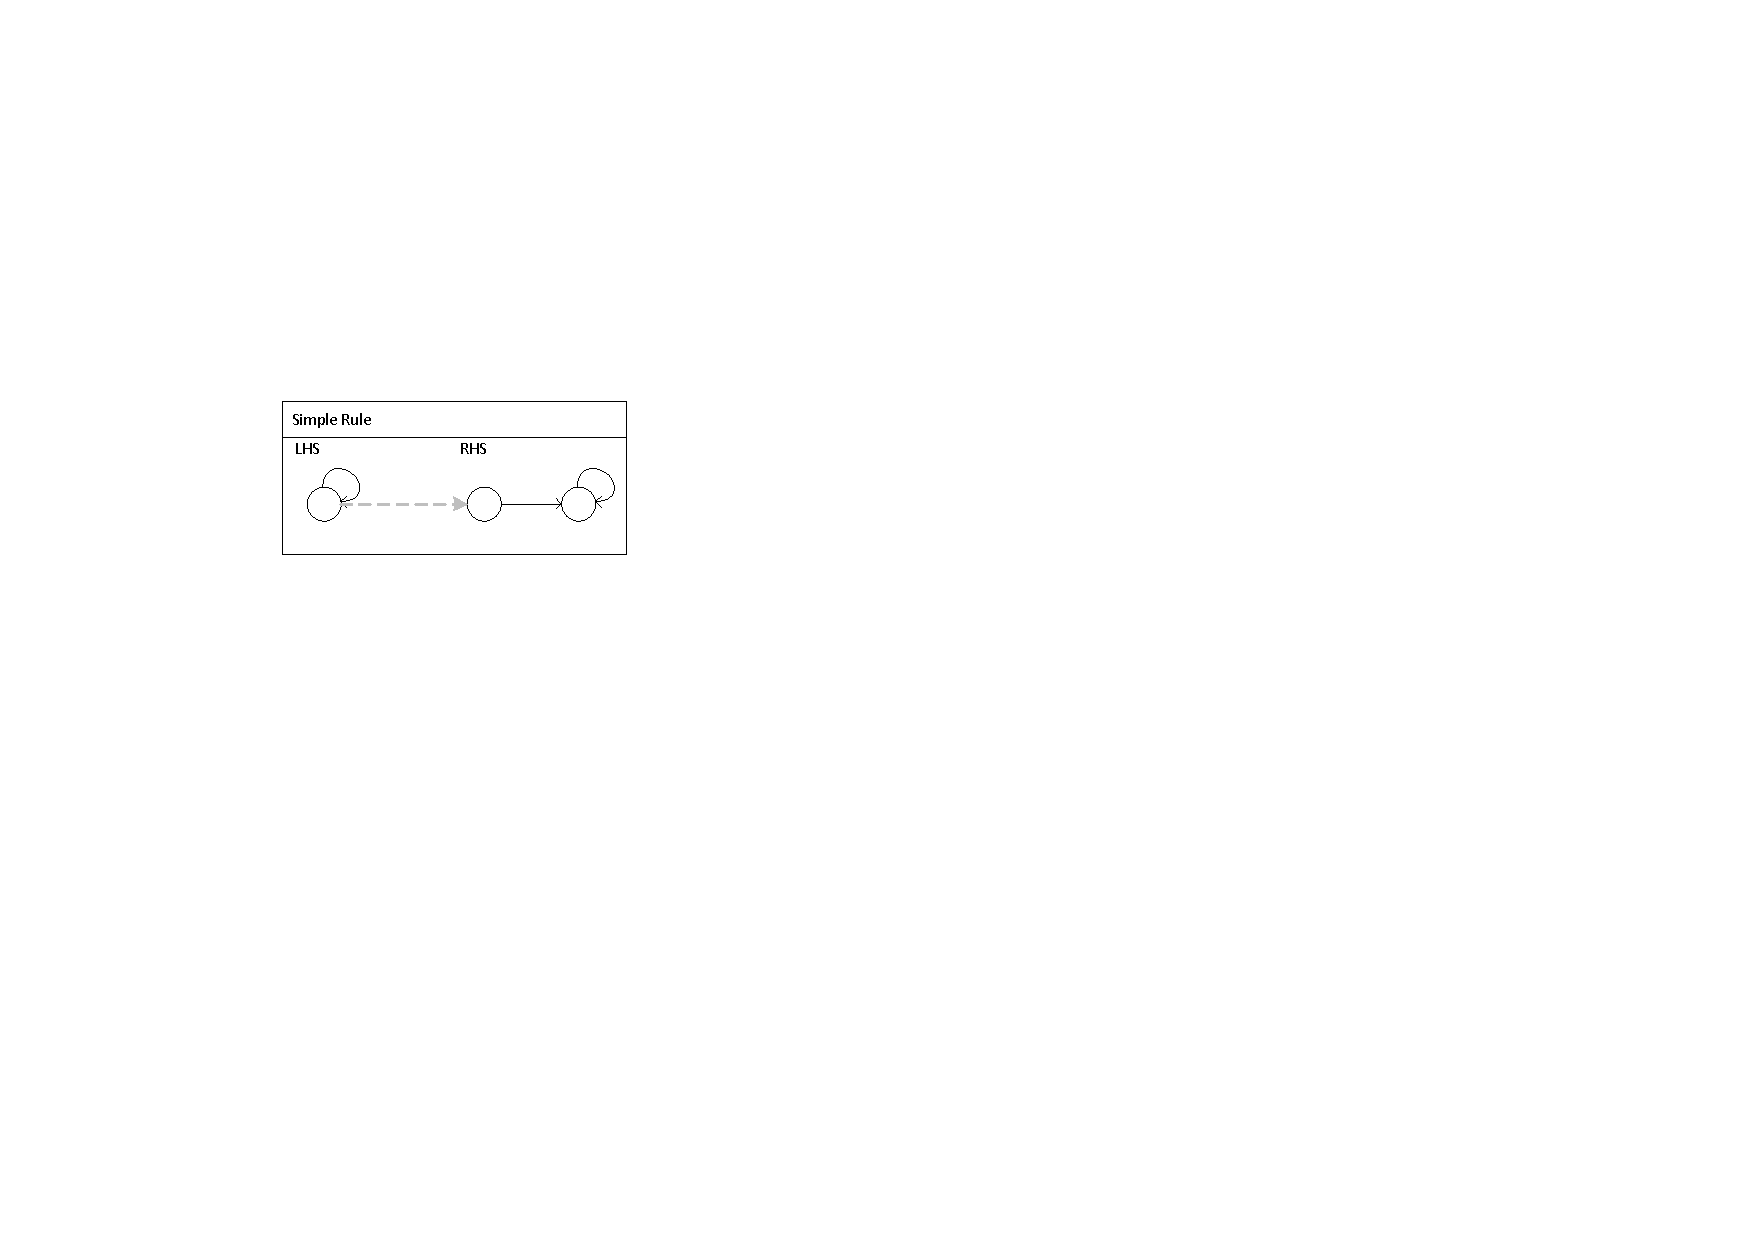
\includegraphics[scale=1.5]{figures/SimpleGTRule}
  \caption{Simple Graph Transformation Rule}
  \label{fig:simpleGTRule}
\end{figure}

Figure \ref{fig:simpleGTRule} shows an example of a graph transformation rule. The LHS contains only node node with a self-edge. The RHS contains two nodes connected by an edge where the right node of the RHS has a self-edge as well. The rule morphism is visualized by the grey, dotted arrow. It specifies that the node of the LHS and the left node of the RHS are considered to be the same.

The application of a graph transformation rule to a graph is called a \emph{graph transformation} \cite{EEPT06}. The graph on which the rule is to be applied is called the \emph{host graph}.
The application of a graph transformation rule to a graph is performed in three steps. In the first step, an occurrence of the LHS of the graph transformation rule in the host graph is searched. Such an occurrence is called a \emph{match} of the graph transformation rule. If a match has been found, all nodes and edges that occur in the LHS but not in the RHS are deleted from the host graph. In this step, the rule morphism is used to decide which nodes do not occur in the RHS. In the third step, all nodes and edges that occur in the RHS but not in the LHS are added to the host graph. After the application of the graph transformation rule, there exists a match of the RHS into the host graph.

\begin{figure}[htbp]
  \centering
  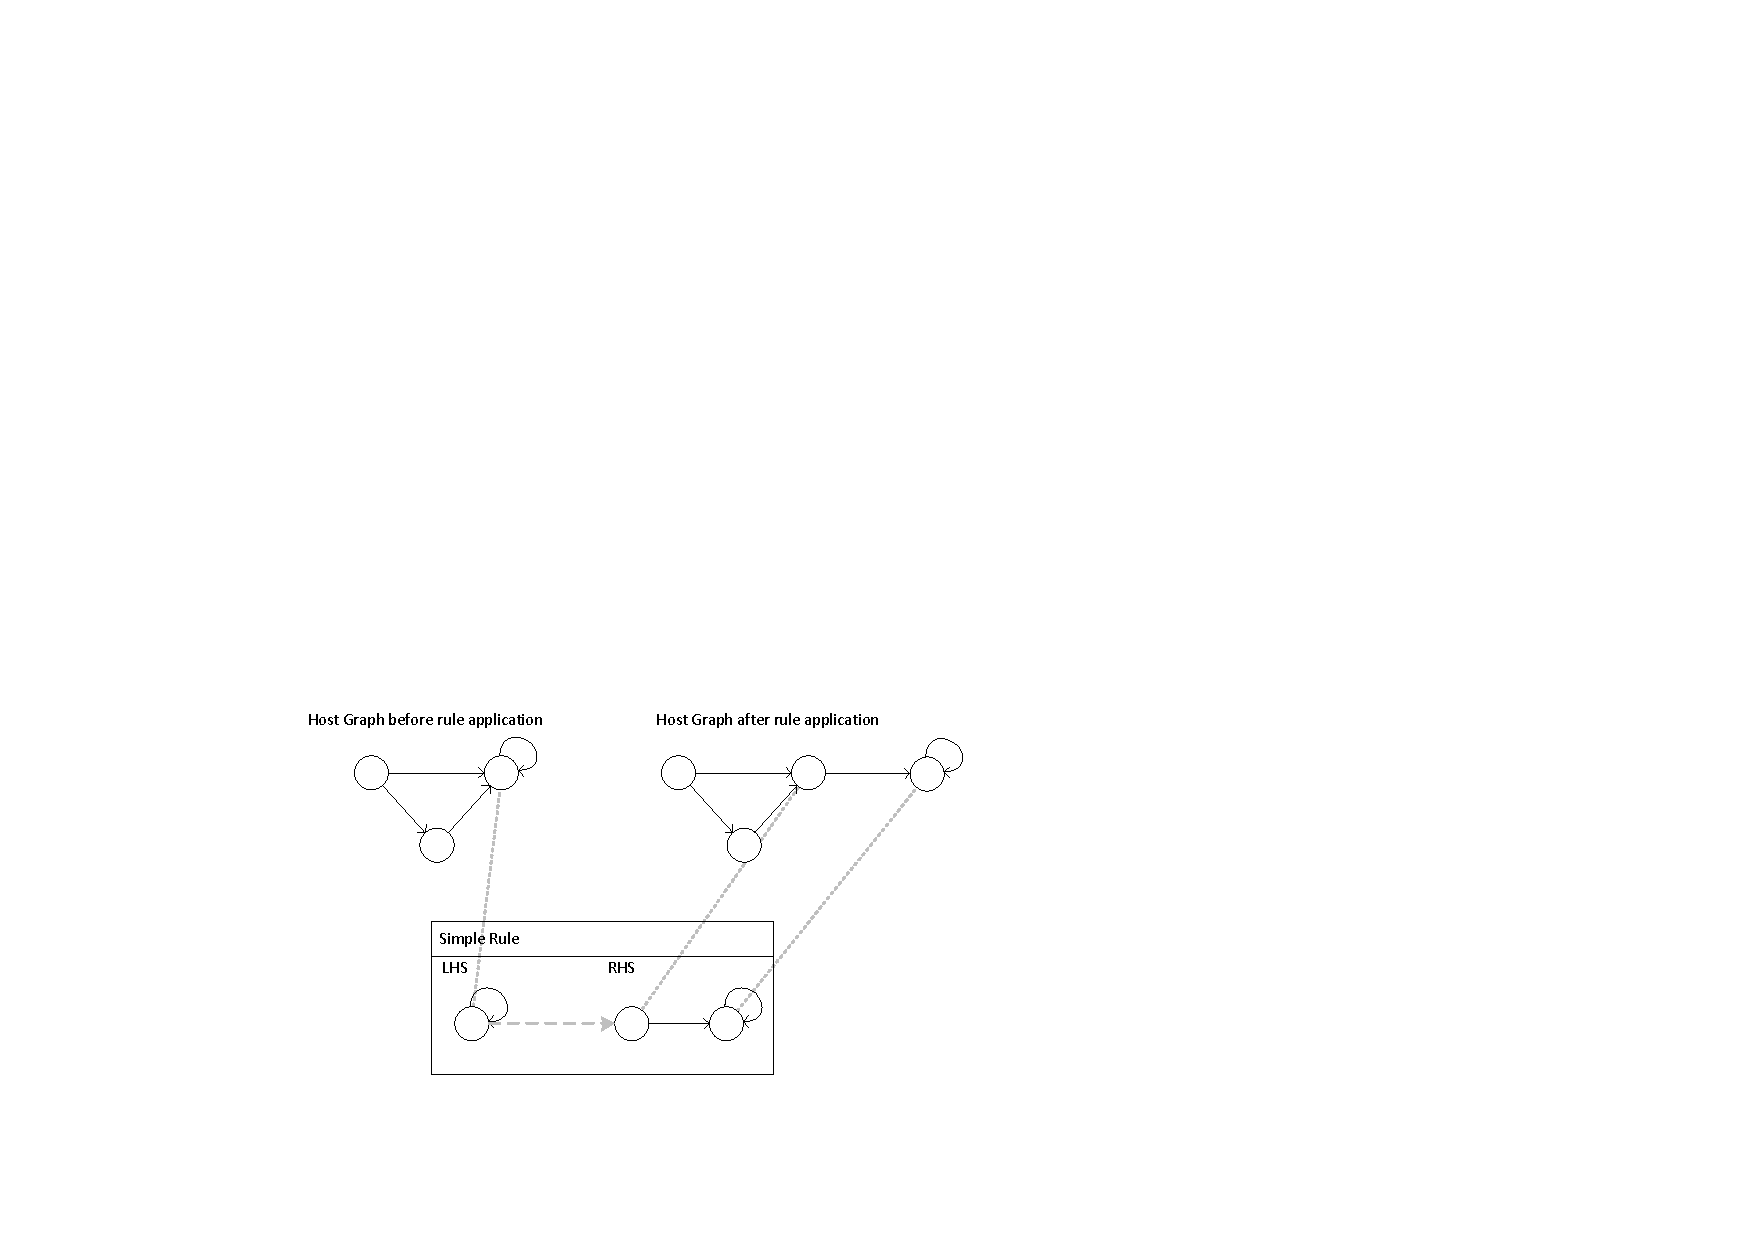
\includegraphics[width=\linewidth]{figures/GTApplication}
  \caption{Application of a Graph Transformation Rule}
  \label{fig:GTApplication}
\end{figure}

Figure \ref{fig:GTApplication} shows an example of a graph transformation that applies the graph transformation rule of Figure \ref{fig:simpleGTRule} to the graph of Figure \ref{fig:simpleGraph}. The matching of the LHS into the host graph is visualized by a gray, dotted line. Then, the graph transformation rule deletes the self-edge from this node. Afterwards, a new node with a self-edge is created and connected to the previously matched node by an edge. The match of the RHS into the host graph after the rule application is again shown by gray, dotted lines.

In the field of algebraic graph transformations, the two most popular approaches for applying a graph transformation rule to a graph are the
\emph{double-pushout approach} \cite{Roz97} and the \emph{single-pushout
approach} \cite{Roz97}. The definition of story diagrams follows the
single-pushout approach. Besides the more theoretical differences the two
approaches differ in the handling of two special situations that might occur
upon rule application.

The first situation is the following. Assume the left-hand side of a rule
consists of two nodes. The first node is to be deleted and the second one is
to be preserved. Both of these nodes may be matched to the same node in the host
graph. In this situation, it is not clear if the node in the host graph is to be
deleted or preserved. The double-pushout approach explicitly forbids the application of the rule in such
situations. The single-pushout approach allows such situations and gives
deletion priority over preservation.

The second situation deals with dangling edges. It occurs if a certain node is
to be deleted but some of its incident edges are to be preserved. The
transformation would lead to a non-valid graph in which the edges would not have
either a source or a target node. The double pushout approach does not allow
such situations and instead requires that incident edges are explicitly
deleted. The single-pushout approach allows such situations and implicitly
deletes edges if one of the source or target nodes are deleted.

In general, matches of graph transformation rules are homomorphisms of the LHS of the rule to the host graph. That allows to match two nodes of the LHS to the same node of the host graph leading to first situation mentioned above. Such situations may be prevented by using isomorphisms for matching the LHS. Then, each node of the LHS must be matched to a unique node of the host graph. Thus, using isomorphic matchings solves the first situation when using single pushouts.

\section{Typed Attributed Graph Transformations}
\label{sec:foundations:typedAttrGTS}

Graphs and according graph transformations as introduced in Section \ref{sec:foundations:simpleGTS} are a very basic approach to modeling behavior. When using graph transformations for modeling behavior for object-oriented software or as a foundation for defining the semantics of modeling languages, it is necessary to distinguish different types of nodes and edges in a graph in order to give them semantics. 

Therefore, story diagrams are based on typed attributed graph transformations \cite{EEPT06}. Typed attributed graph transformations introduce a type graph and node attributes. The type graph defines different types of nodes and edges and it defines which types of edges are allowed for which type of nodes. Additionally, nodes may carry attributes like, e.g., objects in an object-oriented programming language. Accordingly, the type graph specifies inheritance relations between types of objects which are also known from object oriented programming languages.

If the graph transformation transforms a model based on a given type graph into a model based on the same type graph, the transformation is called \emph{endogenous}. Otherwise, i.e., the transformation transforms a model based on a given type graph into a model based on another type graph, the transformation is called \emph{exogenous.} Story diagrams are endogenous graph transformations.

\section{Type Graph used in this Report}

\begin{figure}[htbp]
  \centering
  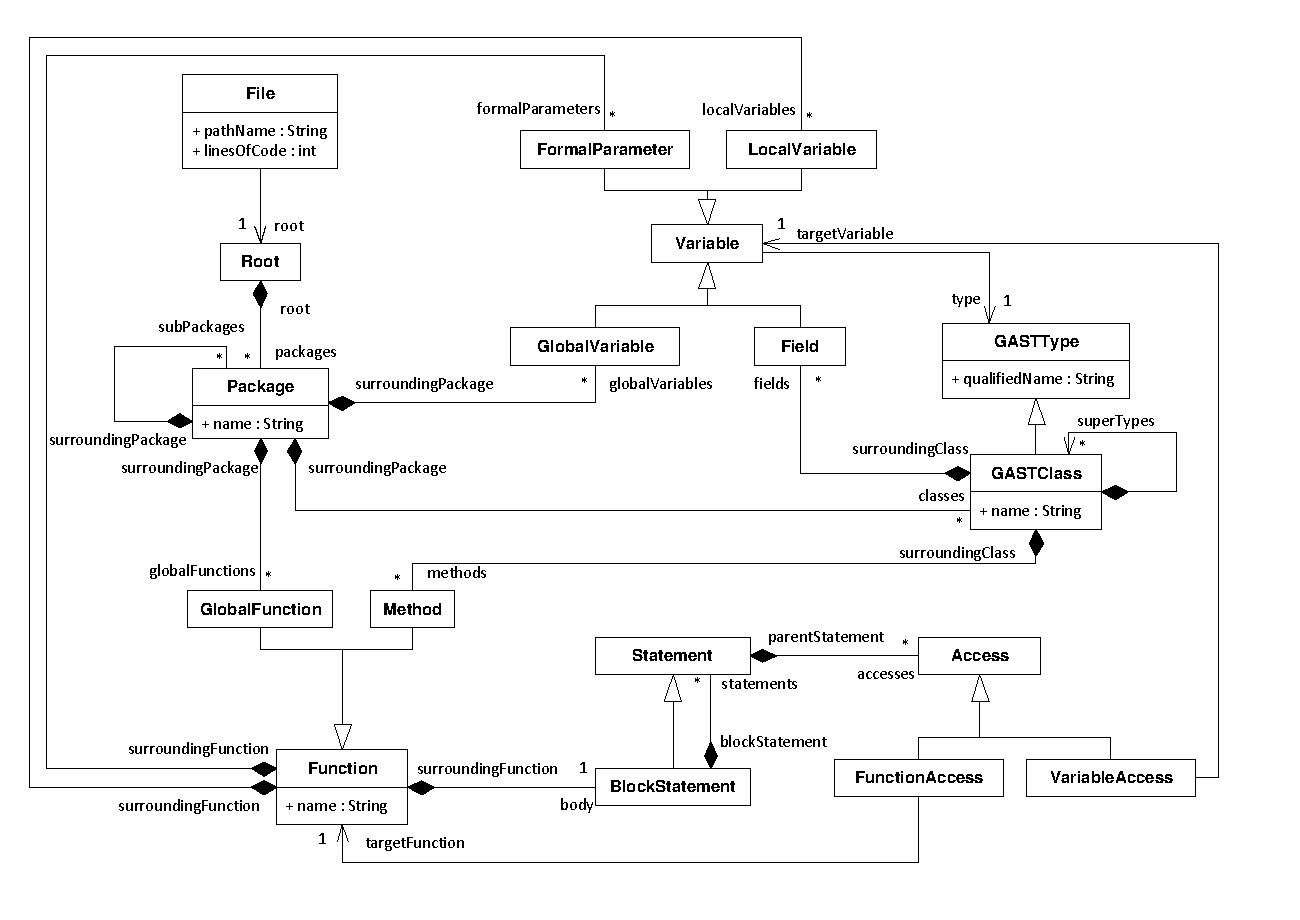
\includegraphics[width=\linewidth]{figures/gast-mm}
  \caption{Type graph of a generalized abstract syntax tree (GAST).}
  \label{fig:gast-mm}
\end{figure}

The type graph used in the examples in this report describes the structure of an abstract syntax tree. In particular it is an updated and slightly simplified version of the generalized abstract syntax tree (GAST) meta model developed in the QBench project \cite{QBench}. The GAST was developed to provide a unified syntax tree model for different programming languages like Java, C, and C++.
Figure~\ref{fig:gast-mm} shows an excerpt of that meta model. Especially some specialized sub classes have been omitted for clarity reasons.

\begin{description}
\item[Root] The \fe{Root} element is the central element of every GAST model. All other elements are reachable from the \fe{Root} node via composition relations.
\item[File] Elements of the GAST, e.g., classes and packages, can be assigned to files in the file system. A \fe{File} element holds references to those classes and packages and a String containing the path to the file.
\item[Package] Similar to packages in Java, the \fe{Package} element provides name spaces and visibilities. A \fe{Package} element can contain other packages, classes, global variables, and functions.
\item[GASTType] The \fe{GASTType} element represents data types like primitive data types and classes. The attribute \fe{qualifiedName} contains the unique, fully qualified name of the type.
\item[GASTClass] Classes are represented by the element \fe{GASTClass} in the GAST and are a sub type of the \fe{GASTType}. A \fe{GASTClass} holds references to its methods, attributes, and inner classes. A \fe{GASTClass} can be assigned to a \fe{Package}.
\item[Function] \fe{Function} is the super type for all executable operations. In addition to a name attribute, a \fe{Function} can have a number of local variables and formal parameters. The return type of a \fe{Function} is determined by its \fe{DeclarationTypeAccess}, a sub class of \fe{Access} (not shown in Figure~\ref{fig:gast-mm}). A \fe{Function} always contains a block statement which, in turn, can contain other statements.
\item[GlobalFunction] A \fe{GlobalFunction} element represents a globally accessible operation, i.e., an operation that does not belong to a class. They can be assigned to a name space defined by a package. For example, C functions are represented by \fe{GlobalFunctions}.
\item[Method] Functions that belong to an class are represented by \fe{Method} elements, a sub type of \fe{Function}.
\item[Variable] \fe{Variable} is a super type for all kinds of variables. A \fe{Variable} always has a name and a type.
\item[LocalVariable] \fe{LocalVariables} are variables that are contained in a \fe{Function}.
\item[FormalParameter] \fe{FormalParameters} are variables that represent the parameters of a \fe{Function},
\item[GlobalVariable] \fe{GlobalVariables} are variables that are globally accessible within a given scope. The scope is determined by the package in which the \fe{GlobalVariable} is contained.
\item[Field] The \fe{Field} element represents class variables. Therefore it is contained in a \fe{GASTClass}.
\item[Statement] A \fe{Function} consists of a number of \fe{Statements}. There are multiple sub classes of \fe{Statement} which represent the different kinds of statements. Most of them are omitted here. A \fe{Statement} can contain a number of \fe{Accesses}.
\item[BlockStatement] The \fe{BlockStatement} is a special kind of statement which can contain other \fe{Statements}. It is the root element of all \fe{Statements} contained within a \fe{Function}.
\item[Access] An \fe{Access} represents the use of a \fe{Variable} or a \fe{Function}. It always belongs to a certain \fe{Statement}.
\item[FunctionAccess] A \fe{FunctionAccess} represents the use of a \fe{Function} in a \fe{Statement} and therefore references the accessed \fe{Funtion} element.
\item[VariableAccess] A \fe{VariableAccess} represents the use of a \fe{Variable} in a \fe{Statement} and therefore references the accessed \fe{Variable} element.
\end{description}


	\chapter{Concepts} \label{sec:Concepts}

\todoall{Description of elements should follow this structure: What is it for? What does it do? Examples in concrete syntax + explanation}

\section*{Old stuff from rejected paper}
In this section, we will briefly introduce story diagrams and their current features. 
Story diagrams combine
UML activity diagrams and graph transformations by embedding graph replacement rules into the activities.
This allows the activities in Figure \ref{fig:transformationOverview} to be specified formally by graph replacements while preserving the general control flow structure of the example transformation.

In terms of the classification of model transformations proposed by Czarnecki and Helsen~\cite{Czarnecki06}, story diagrams are an endogenous, in-place transformation language.
It has both declarative (pattern matching) and operational elements (specification of control flow):
Its control flow allows a deterministic selection of the graph replacement rules to be applied, with a (non-deterministic) pattern matching in the graph replacement rules.
It can also be used for inter-model transformations to create a new target model from a given source model, as seen in the example given in this paper. 
In order to execute story diagrams, code generation \cite{GBD07} and interpretation \cite{GHS09} are supported.

In the following, we will describe the graph transformations, the so-called story patterns, in Section~\ref{sec:StoryPatterns}.
Afterwards, we will explain how control flow can be modeled by using elements from activity diagrams in Section~\ref{sec:StoryDiagrams}.

	\section{Story Diagrams and Story Patterns in a Nutshell (Dietrich \& Jan)} \label{sec:Overview}

%- model-driven software development, raise abstraction level and use models instead of code as the key artifact
%- specify structure and behavior of the software under development, make the models runnable/executable
%- UML offers notations for description of software structure and development, esp. class and activity diagrams
%- activity diagrams are too informal to be automatically executed (natural language used)
%- we replaced the informal activity descriptions with formal descriptions of operations on object structures and developed a new formal language called story diagrams

%- story diagrams are special UML activity diagrams
%- developed to formalize the description of a software's behavior (UML activity diagrams usually use informal textual descriptions of the tasks to be performed)
%- motivation: complete specification of a software, structure and behavior, i.e. make the software specification executable (code generation and interpretation)

In model-driven software development, a software model is the key artifact of the development.
It describes the software's structure as well as its behavior and 
can be translated into executable source code or be interpreted to be executed.
The UML offers notations for the description of the software structure and behavior,
besides others class diagrams and activity diagrams.
However, since UML activity diagrams use natural language in the activity nodes to describe the particular activities, they are not automatically executable.
Thus, a formal behavioral specification is needed.
For that purpose, \emph{story diagrams} have been developed \cite{FNTZ00,Zun01}.
They are based on UML 1.5 activity diagrams \cite{UML1.5} and replace the natural language with a formal language to specify behavior
and, thus, can be automatically executed.

In terms of the classification of model transformation languages proposed by Czarnecki and Helsen \cite{Czarnecki06},
story diagrams are an endogenous, in-place transformation language (see also Section~\ref{sec:foundations:typedAttrGTS}).

%- motivation: (formally) describe modifications of object structures for object-oriented software systems
%- use a graphical notation to specify operations on object structures (object structure modifications), OO world
%- each operation describes a modification of a given object structure, basically the modifactions are creations and removals of objects and their interconnections
%- graphically describe the object structure to be modified, mark the elements to be created and those to be removed

Story diagrams describe the control flow similar to UML activity diagrams by means of activity nodes and activity edges.
The behavior of each activity node is described using a graph transformation language called \emph{story patterns}.
Each activity node embeds one story pattern.
A story pattern uses a graphical notation to specify modifications of object structures in object-oriented software systems.
The modifications are basically creations and removals of objects and their interconnections (links).

%- motivation: use an appropriate, familiar, and simple notation for object structure modifications; we use a notation similar to UML object diagrams
%- motivation: declaratively describe the operations in activity nodes, thus, reduce complexity (avoid describing how to perform the operations)
%- motivation: keep determinism to a certain extent to specify the conditions for and the order of object structure modifications

Using a simple and familiar notation, story patterns are similar to UML object diagrams (see the embedded story pattern in Figure~\ref{fig:SDExampleStoryDiagram}).
A story pattern represents an object structure that is to be modified.
It includes annotations specifying which objects and links are to be removed and created.
Story patterns are a declarative language since they only specify what to remove and create but not how to do it and in which order.
This way, the complexity of the behavioral specifications is reduced.
In contrast to the deterministic control flow specified by activity nodes and edges which determine the order of story pattern executions,
the order of creations and deletions specified by a story pattern is non-deterministic.

%- motivation: base the specification on a well-known formalism (for execution and analyses)
%- story diagrams use graph transformations in their activity nodes (well-known formalism, exhaust the given theories for analyses and execution)

Story patterns are based on the well-known formalism of \emph{graph transformation systems} and the corresponding theory \cite{Roz97}.
Thus, precise analyses of the operations described by story patterns are possible,
e.g., it can be checked if certain properties of the object structure to be modified remain after the structure's modification \cite{Sch06,Mey09}.

%- given a so called host graph (an object structure or model), story diagrams describe the graph's modifications by means of creating or removing nodes and edges (objects and links)
%- the host graph, in our case, is a typed attributed graph, i.e. we have a graph to be modified (object structure, token model) and a corresponding type graph (type model or meta-model) describing the types and properties of the objects in our host graph
%- a graph transformation is executed by identifying a subgraph in the host graph which corresponds to the graph specified in the transformation (matching, subgraph isomorphism), removing nodes and links that are marked to be removed, and creating new nodes and links that are marked to be created

A story pattern specifies a graph transformation \cite{Roz97}.
Given a so-called \emph{host graph}, i.e.\ the graph to be modified, a graph transformation removes and creates nodes and edges in the given host graph.
The host graph is a typed attributed graph, i.e.\ there is a \emph{type graph} determining the types and attributes of the nodes.
A graph transformation is executed on a host graph by identifying a subgraph in the host graph that is similar to the one specified in the graph transformation
and then removing and adding the specified nodes and edges.
The identification of the subgraph for modification is called \emph{graph matching} and includes the \emph{subgraph isomorphism} problem
(see Chapter~\ref{sec:foundations} for more details).

In case of story patterns, the host graph is the object structure or model to be modified, i.e.\ the run-time data of the executed software.
Thus, we call the host graph's nodes and edges \emph{objects} and \emph{links}
while the host graph itself is called \emph{instance model}\footnote{Thomas K\"{u}hne calls it \emph{token model} \cite{Kue06}.} (or simply model) in the remainder of the report.
The type graph is a set of classes and their relations which define all potential instance models at run-time.
These classes and relations constitute a so-called \emph{type model} or the \emph{metamodel} \cite{Kue06} of the language used to describe instance models.
Furthermore, we call the nodes and edges in story patterns \emph{object variables} and \emph{link variables}
since these represent and are matched to objects and links in the instance model.
The types of these variables are determined by types in a type model which is required to specify story patterns.

\begin{figure}[htb]
	\centering
  \begin{minipage}[t]{.4\textwidth}
    \centering
    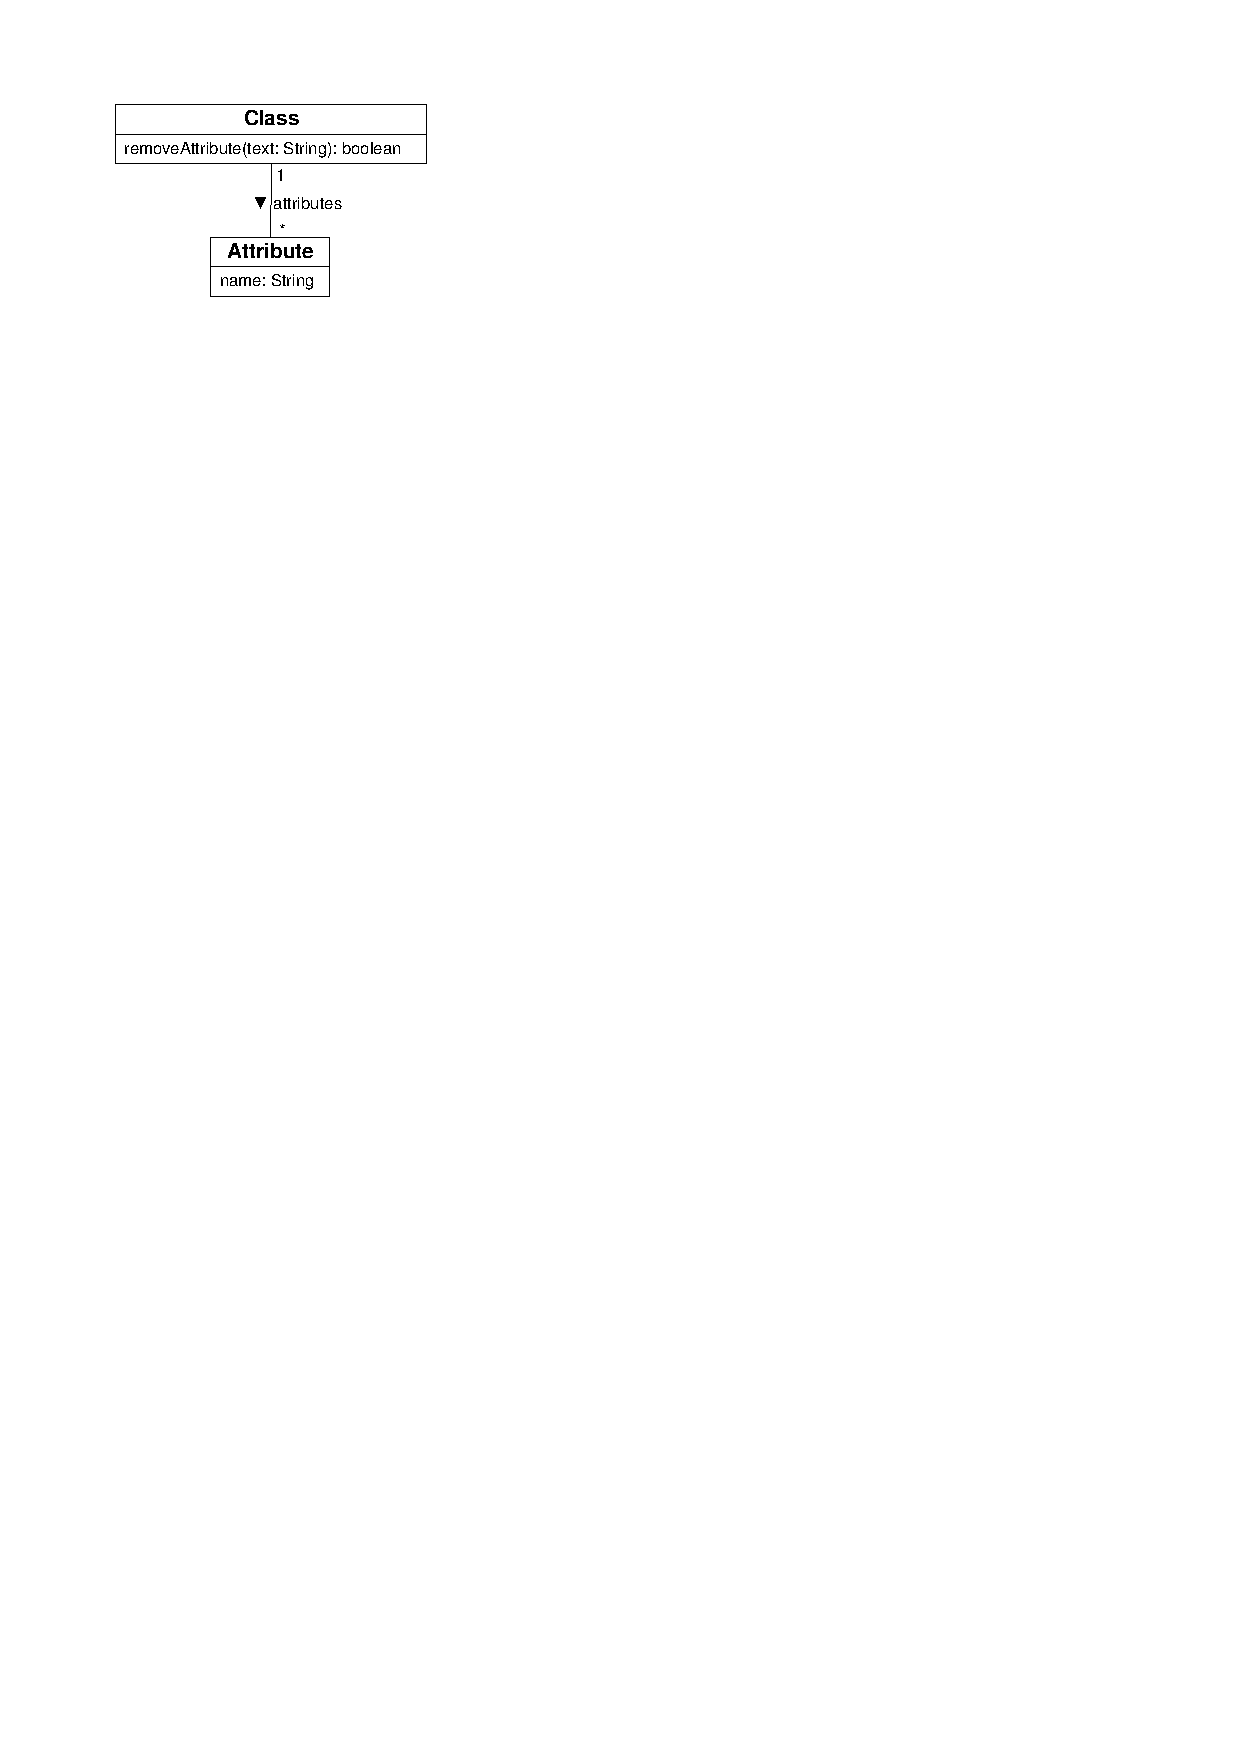
\includegraphics[scale=1]{SimpleSDRemoveAttributeClassDiagram} 
    \caption{Exemplary Type Model}
    \label{fig:SDExampleClassDiagram}
  \end{minipage}%
  \hfill
  \begin{minipage}[t]{.55\textwidth}
    \centering
    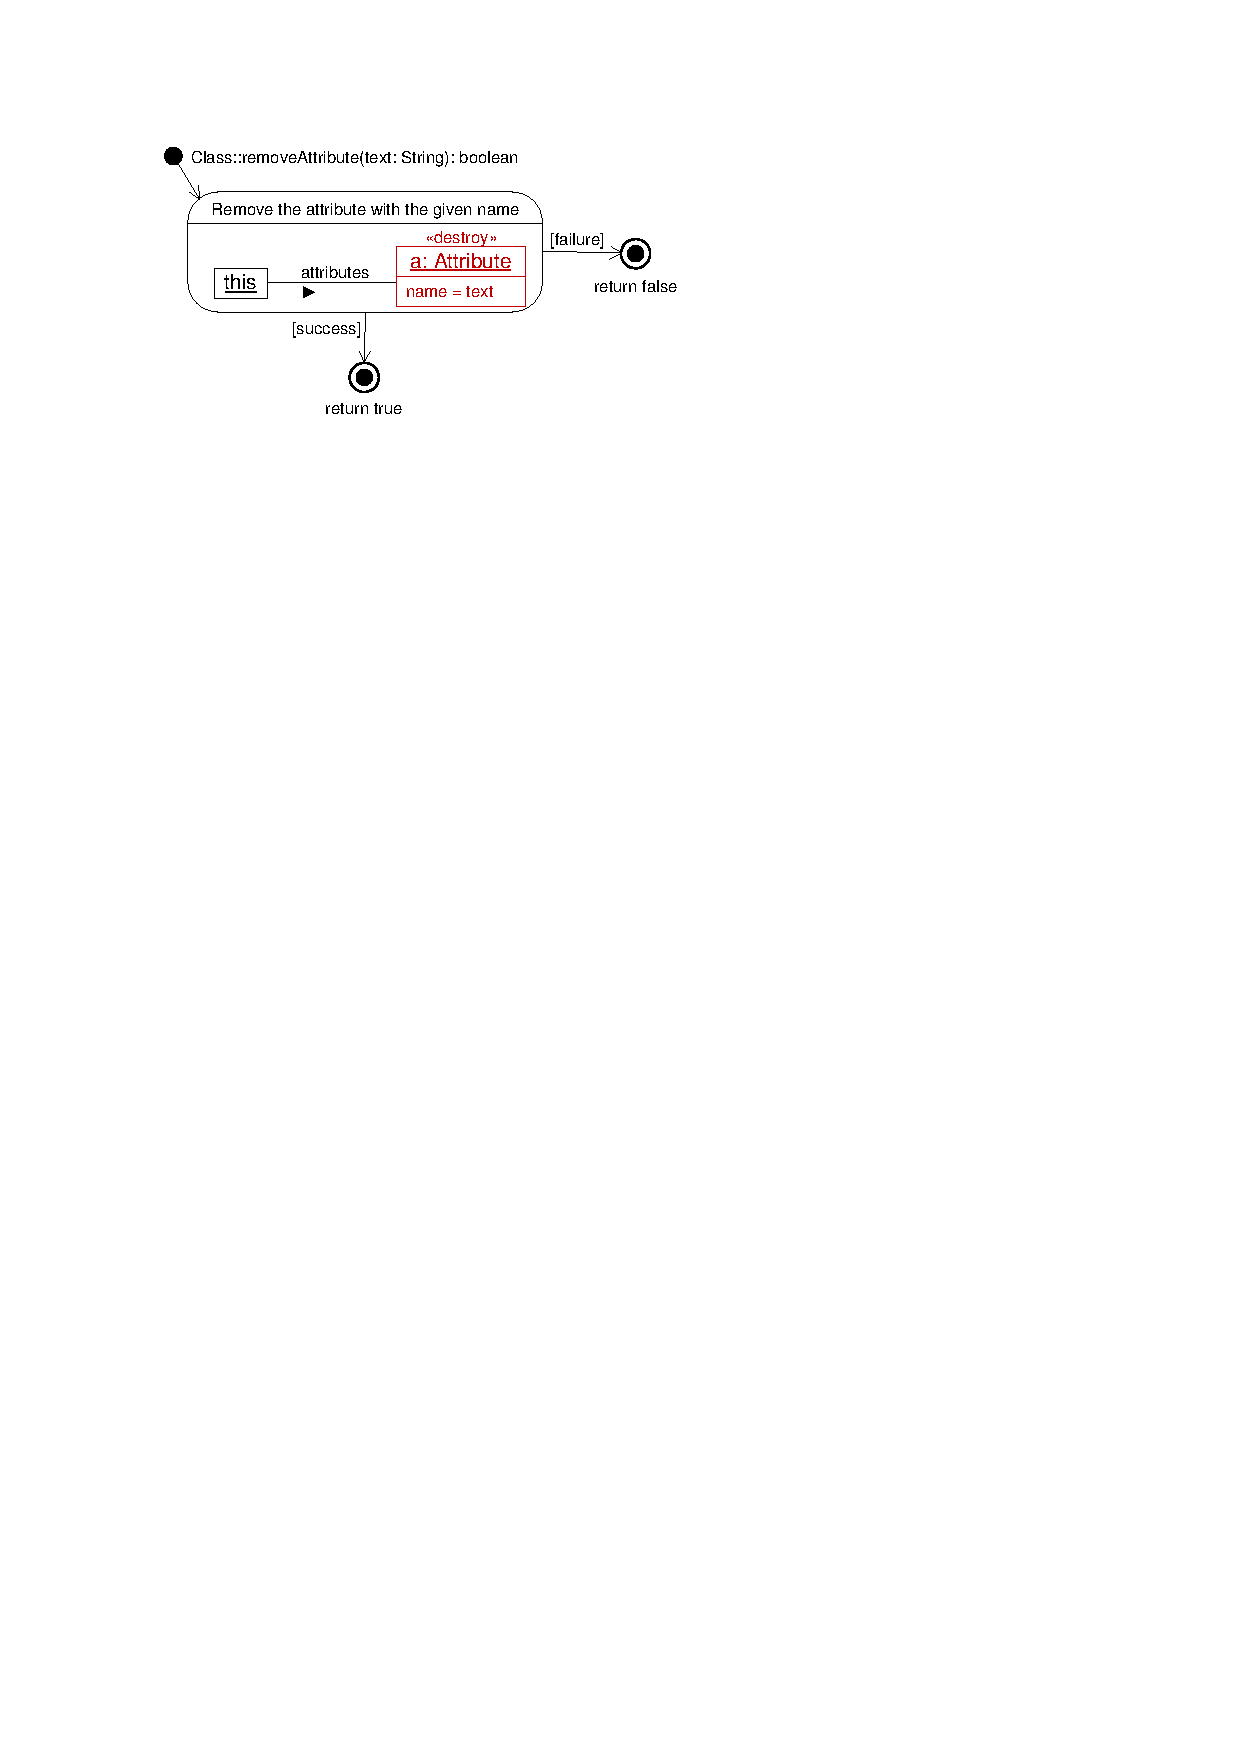
\includegraphics[scale=1]{SimpleSDRemoveAttribute}
    \caption{Exemplary Story Diagram}
    \label{fig:SDExampleStoryDiagram}
  \end{minipage}
\end{figure}

For example, the class diagram in Figure~\ref{fig:SDExampleClassDiagram} defines the types \fe{Class} and \fe{Attribute} as well as their relations, attributes, and operations.
The corresponding story diagram in Figure~\ref{fig:SDExampleStoryDiagram} defines the behavior of the \fe{removeAttribute} method defined in the class diagram.
Here, the story diagram specifies that a class's attribute with the name given by the parameter \fe{text} is to be found in the instance model and in case of success this attribute is to be removed (\destroy).

In summary, a story diagram is a special, formally defined UML activity diagram
that embeds graph transformations, so-called story patterns, in its activity nodes
to precisely describe run-time behavior by means of graph transformations.

%\subsection{Application scenarios (?)} \label{sec:Applications}

	\section{Story Patterns} 
\label{sec:StoryPatterns}

In this section, we introduce story patterns in more detail.
We start by giving the general idea of story patterns in Section \ref{sec:StoryPatterns:storyPattern}.
Thereafter, we describe the basic concepts of story patterns, namely object variables, link variables,
and their respective binding semantics in Sections \ref{sec:StoryPatterns:objects} to \ref{sec:StoryPatterns:binding}.
Finally, we show the use of object attributes in a story pattern in Section \ref{sec:StoryPatterns:attributes}.


\subsection{General Idea}
\label{sec:StoryPatterns:storyPattern}

Story patterns are typed attributed graph transformation rules with inheritance on object types (cf. Section~\ref{sec:foundations:typedAttrGTS}) that can be embedded into an activity node of a story diagram (cf. Section~\ref{sec:StoryDiagrams}).
 By using a type model as introduced in Section~\ref{sec:foundations:typedAttrGTS}, story patterns enable polymorphism for matching object and link variables.
This allows for specifying graph replacement rules for object-oriented models.

Object and link variables are matched to the objects and links of the instance model. 
In contrast to typed attributed graph transformations, story patterns explicitly require to use isomorphic matchings, i.e., two object variables of a story pattern may not be matched to the same object of the instance model.

For enabling a concise notation of the graph transformation, story patterns apply a short-hand notation depicting the left-hand side (LHS) and the right-hand side (RHS) in a single, annotated graph using stereotypes.
In the short-hand notation, we use binding operators for defining the LHS and the RHS. Object and link variables representing objects and links not to be changed by the story pattern carry no stereotype. 
Object and link variables representing objects to be created (or deleted) are annotated with \create (or  \destroy, respectively). 
Consequently, the LHS consists of all object and link variables that carry no stereotype or stereotype \destroy. The RHS consists of all object and link variables that carry no stereotype or the stereotype \create.
The deletion of objects and links follows the single-pushout approach (cf.\ Section~\ref{sec:foundations:simpleGTS}).

Figure \ref{fig:simpleStoryPattern} shows an example of a single story pattern that redirects a method call from an old method to a new method.
\begin{figure}[htb]
  \centering
  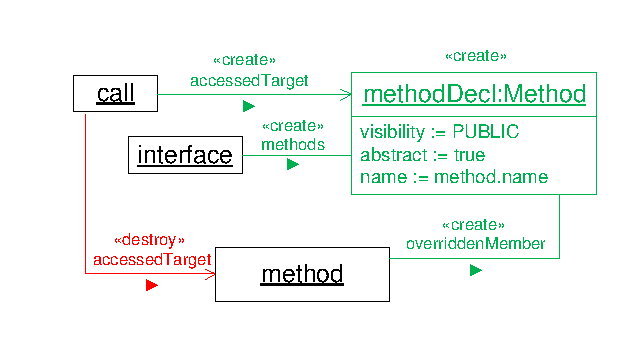
\includegraphics[scale=1.0]{figures/SimpleStoryPattern}
  \caption{Example of a Story Pattern}
  \label{fig:simpleStoryPattern}
\end{figure}
In the example, the object variables \fe{parentClass}, \fe{oldMethod}, and \fe{newMethod} are bound variables, i.e., they already refer to objects of the instance model (cf. Section \ref{sec:StoryPatterns:binding:states}).
The object variables \fe{anyMethod} and \fe{c} are unbound. 
When applying the story pattern, first a match for \fe{anyMethod} and \fe{c} is searched in the instance graph. 
A possible match will be any method in \fe{parentClass} which contains a call to \fe{oldMethod}. 
If the matching is successful, the link from \fe{c} to \fe{oldMethod} will be deleted and the link from \fe{c} to \fe{newMethod} will be created.

In the concrete syntax of story patterns, the object and link variables representing objects and links not to be modified by the story pattern are visualized in black. 
Object and link variables representing objects and links to be destroyed are annotated with \destroy and visualized in red. 
Object and link variables representing objects and links to be created are annotated with \create and visualized in green. 
An unbound object variable is labeled with its name and the name of the corresponding type. 
For bound object variables, we omit the name of the type (e.g., \fe{parentClass} in Figure~\ref{fig:simpleStoryPattern}).

In general, the matching process is executed as a three step process:
first, a matching is searched which uses the bound variables of the story pattern as a starting point. The matching associates objects and links of the instance model to all object and link variables of the story pattern. 
The matching is performed as defined for typed attributed graph transformations and considers all object and link variables of the LHS.
If a matching can be obtained, the story pattern is applicable and the execution proceeds. 
\tododt{What happens if the modification operations are contradictory (see Section~\ref{sec:DecisionNodesEtc})?}
Otherwise the execution of the story pattern is aborted.
In the second step, all objects and links matched to object and link variables annotated with \destroy are deleted. 
Finally, objects and links are created in the instance model for all variables annotated with \create.

Story patterns aim to reduce the computational complexity of the matching process (cf. Section~\ref{sec:foundations:simpleGTS}) by using bound variables.
We require at least one bound object variable in each story pattern which is used as a starting point for the matching process.


\subsection{Objects and Object Variables}
\label{sec:StoryPatterns:objects}

Object variables in a story pattern represent the objects in an instance model to be matched.
The variables are uniquely identified by their name.
The objects are instances of classes of the underlying type model (cf.
Section \ref{sec:foundations:typedAttrGTS}). Thus, the object variables are typed by classes from this model.

The story pattern in Figure \ref{fig:simpleStoryPattern} contains five
object variables with the names \fe{parentClass}, \fe{oldMethod}, \fe{anyMethod}, \fe{c} and
\fe{newMethod}. 
The type of an object variable is only visualized if the
variable is unbound or maybe bound (cf.\ Section
\ref{sec:StoryPatterns:binding:states}). For example, the object variable \fe{anyMethod} has the type \fe{Method}.

Object variables have binding states, binding operators and binding semantics which are described in Section  \ref{sec:StoryPatterns:binding}.


\ext %--- Comment this line to include primitive variables into the document
{
\todomcp{Primitive Variables: concrete syntax like
object variables; binding expressions for initialization, see figure
\ref{fig:primitiveVariable}; primitive variables are typed over EDataType; they
exist to the end of the Activity}

\begin{figure}[htb]
  \centering
  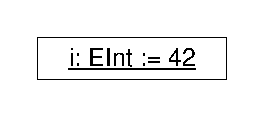
\includegraphics[scale=0.6]{figures/PrimitiveVariable}
  \caption{Primitive variable with value assignment}
  \label{fig:primitiveVariable}
\end{figure}

\todomcp{Links to primitive variables: special LinkVariable, typed over
EStructuralFeature}
}%------ End of primitive variables section



\subsection{Links and Link Variables}
\label{sec:StoryPatterns:links}

Link variables represent connections between objects and are used to connect
different object variables.
A link variable is typed over a reference of the underlying type graph.
\tododt{The typing should be described more precisely.
The link variable is typed over one or two corresponding \fe{EReferences} that conceptually represent a uni-directional or bi-directional association.}

Like object variables, link variables also have binding
operators and binding semantics (cf. Section \ref{sec:StoryPatterns:binding}), but no binding state.




\subsection{Binding of Variables}
\label{sec:StoryPatterns:binding}

Object variables have binding states (unbound, bound, maybe
bound), binding semantics (mandatory, negative, optional), and binding operators
(check only, create, destroy). Link variables have binding
operators and binding semantics.
Their meaning is described in the following. 


\subsubsection{Binding States}
\label{sec:StoryPatterns:binding:states}

An object variable or a link variable can be declared as \emph{bound}, \emph{unbound}, or
\emph{maybe bound} (i.e., it is unknown if the variable is bound or not). This is
defined by its binding state. An unbound variable is matched during the
execution of the containing story pattern. 
A bound variable must have been matched previously. 
For a variable that is specified as maybe bound, a new match will only be
determined if it has not been bound before. 
Otherwise it will be treated as a bound variable.
This is useful, if the same pattern should be used in different contexts, i.e., the bound variable of the pattern differs depending on the context but otherwise the patterns are identical.
Without maybe bound variables, different patterns would have to be modeled that only differ in which variable is the bound variable of the pattern.
With maybe bound variables, all variables can be set to maybe bound and the caller specifies a binding for one of them depending on the context.
%\todomcp{explain why maybe bound is necessary}

Unbound object variables are visualized with an underlined label of the form
``name: Type'' (cf. Figure \ref{fig:bindingStatesOverview} a)).
For bound object variables the type is hidden, as depicted
in Figure \ref{fig:bindingStatesOverview} b).
Maybe bound object variables are represented like unbound object variables, but
are marked by a question mark after the name (cf.\ Figure
\ref{fig:bindingStatesOverview} c)).

In a valid story pattern, each connected component\footnote{With
``connected component'' we mean a subgraph in which each object variable is
reachable from at least one bound object variable via directed link variables.}
must contain at least one bound object variable or created variables only. This
is necessary to avoid a search over the whole underlying instance model which requires a long runtime in most cases (cf. Section~\ref{sec:StoryPatterns:storyPattern}).

\begin{figure}[htb]
  \centering
  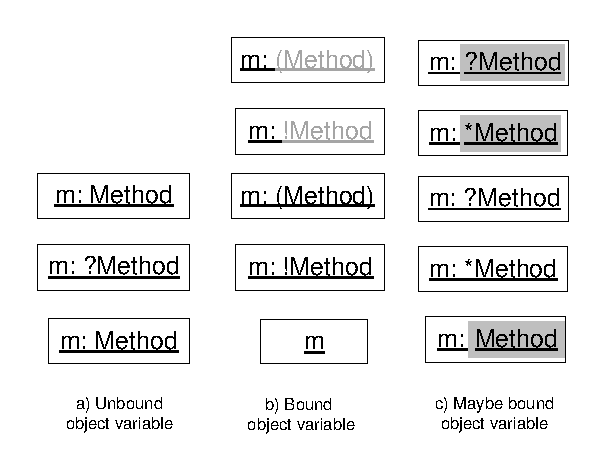
\includegraphics[scale=1.2]{figures/BindingStatesOverview}
  \caption{Binding States for Object Variables}
  \label{fig:bindingStatesOverview}
\end{figure}

\subsubsection{Binding Semantics}
\label{sec:StoryPatterns:binding:semantics}
Object variables and link variables have binding semantics that
determine if a variable is mandatory, negative or optional.
A match for mandatory variables must exist in the given instance model, otherwise
the pattern matching fails. 
In contrast, negative variables constitute so-called negative application
conditions (NACs) and must not exist in the instance model. If a variable defined as
negative can be matched during the execution of the story pattern, the pattern matching
fails. Matches for optional variables may exist. An optional variable will be
bound if possible, but the story pattern may also be matched
successfully otherwise.

Negative object variables are visualized crossed-out (cf. Figure
\ref{fig:bindingSemanticsOverview} b)) and optional object variables are
visualized with a dashed border (cf.\ Figure \ref{fig:bindingSemanticsOverview} c)).
The same holds for negative and optional link variables (cf. Figure
\ref{fig:bindingSemanticsOverview} e) and f)).

Negative as well as optional object and link variables are not part of a
connected component.
This means, the graph has to be still connected when ignoring optional and negative
parts. However, optional and negative object variables must be reachable from a connected component. 
Consequently, regarding the rule that each connected component must
contain at least one bound object variable (cf.\ Section
\ref{sec:StoryPatterns:binding:states}), there are situations in which the
use of negative or optional object variables is not allowed. 
Figure \ref{fig:negativeObjects} shows these situations. 
Case a) is allowed but case b) is not because, in the latter case,
the graph without the negative and optional elements is not a connected component anymore.
Case c) is allowed because the object
variables \fe{a} and \fe{c} are bound which means that each connected component has at least one bound object variable.
Accordingly, case d) is allowed, too, because \fe{a} and \fe{b} are both
bound. Case e) is not allowed while Case f) is.
Case g) is not allowed because the semantics is the same as in Case a) due to the single-pushout approach of story patterns.

Similar to the application of negative object
variables, Figure \ref{fig:optionalObjects} shows some examples for the application of optional object variables. 
While case a) is allowed, case b) is not allowed because in this case the
shown graph is not connected anymore. However, case c) and d) are allowed
because each connected component contains at least one bound object variable.
Cases e) and f) are also allowed.

\begin{figure}[htb]
  \centering
  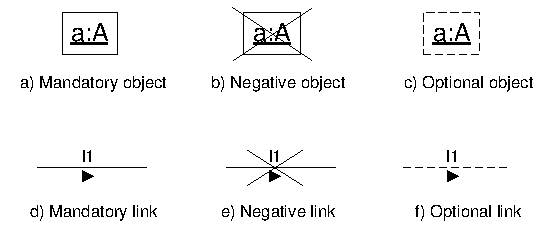
\includegraphics[scale=1.2]{figures/BindingSemanticsOverview}
  \caption{Binding Semantics for Object and Link Variables}
  \label{fig:bindingSemanticsOverview}
\end{figure}

\begin{figure}[htb]
  \centering
  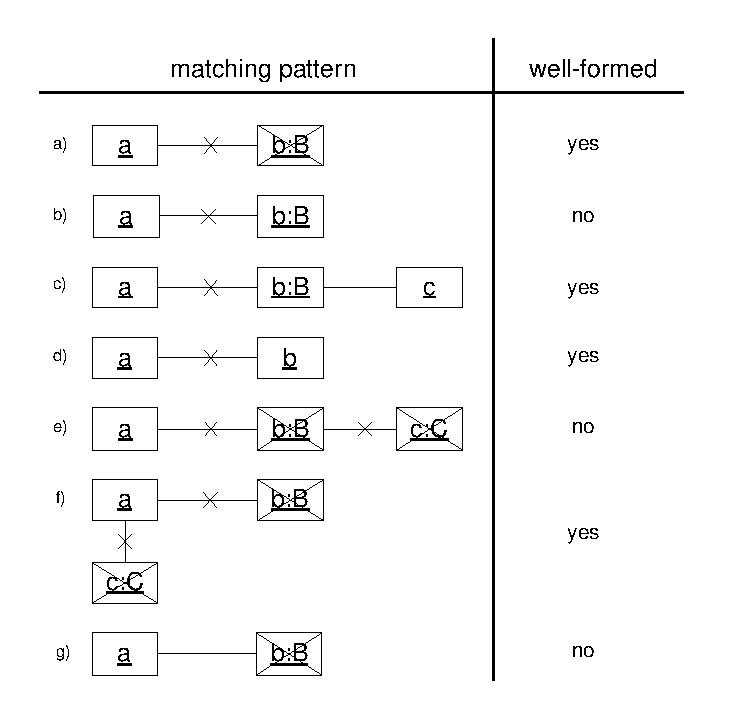
\includegraphics[scale=1]{figures/negativeObjects}
  \caption{Negative Application Conditions}
  \label{fig:negativeObjects}
\end{figure}

\begin{figure}[htb]
  \centering
  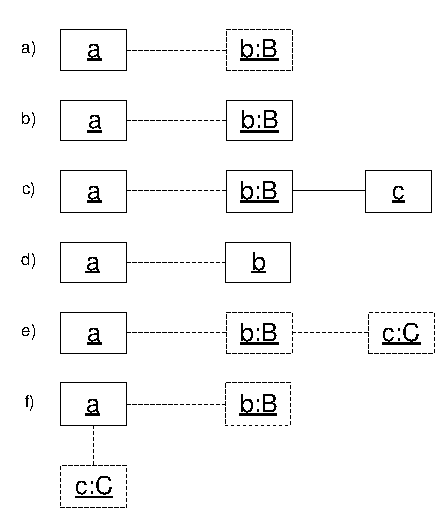
\includegraphics[scale=1]{figures/optionalObjects}
  \caption{Optional Object and Link Variables}
  \label{fig:optionalObjects}
\end{figure}


\subsubsection{Binding Operators}
\label{sec:StoryPatterns:binding:operators}

Binding operators define whether an object or link is to be created, deleted,
or just matched in the instance model.
After all elements that are defined to be deleted or just matched have been
matched, the model is modified by deleting and creating the elements as
defined (see Section~\ref{sec:StoryPatterns:storyPattern}).

It may happen that a matching is successful but that the specified creation is infeasible.
For instance, constraints imposed upon the elements to be created may be contradictory (see Section~\ref{sec:StoryPatterns:linkConstraints:orderConstraint}).
Of course, it is not sensible to specify such constraints but it cannot always be checked statically if constraints are contradictory or not.
If such a situation is detected at execution time, the execution of the story diagram is aborted.

Objects and links to be created are marked with the
stereotype \create (cf.\ Figure \ref{fig:bindingOperatorsOverview} b) and e)) and objects and links
to be deleted are marked with the stereotype \destroy (cf.\ Figure
\ref{fig:bindingOperatorsOverview} c) and f)).

\begin{figure}[htb]
  \centering
  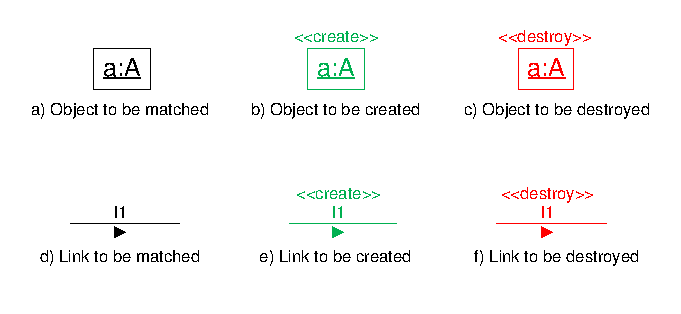
\includegraphics[scale=1.2]{figures/BindingOperatorsOverview}
  \caption{Binding Operators for Object and Link Variables}
  \label{fig:bindingOperatorsOverview}
\end{figure}

Since no objects and links exist for variables marked with \create, they also do not belong to a connected component (like
negative or optional variables).


\subsubsection{Feasible Binding Combinations}

Binding states, binding semantics and binding operators can be
arbitrarily combined, but only certain combinations are feasible. 
Table \ref{tab:bindingCombinations} lists all feasible binding combinations for
object variables. As shown there, bound and maybe bound object variables must not have negative
or optional binding semantics. As well, the combination of the binding states
bound or maybe bound and the binding operator create is not allowed.

% Table generated by Excel2LaTeX from sheet 'Tabelle1'
\begin{table}[htbp]
  \centering
  \caption{Feasible Combinations of Binding States, Binding Semantics, and
  Binding Operators for Object Variables}
    \begin{tabular}{|r|r|r|r|}
    \hline
    \textbf{Binding State} & \textbf{Binding Semantics} & \textbf{Binding
    Operator} & \textbf{Feasible} \\
    \hline
    UNBOUND & MANDATORY & CHECK\_ONLY & yes \\
    UNBOUND & MANDATORY & CREATE & yes \\
    UNBOUND & MANDATORY & DESTROY & yes \\
    UNBOUND & NEGATIVE & CHECK\_ONLY & yes \\
    UNBOUND & NEGATIVE & CREATE & no \\
    UNBOUND & NEGATIVE & DESTROY & no \\
    UNBOUND & OPTIONAL & CHECK\_ONLY & yes \\
    UNBOUND & OPTIONAL & CREATE & yes \\
    UNBOUND & OPTIONAL & DESTROY & yes \\
    \hline
    BOUND & MANDATORY & CHECK\_ONLY & yes \\
    BOUND & MANDATORY & CREATE & no \\
    BOUND & MANDATORY & DESTROY & yes \\
    BOUND & NEGATIVE & CHECK\_ONLY & no \\
    BOUND & NEGATIVE & CREATE & no \\
    BOUND & NEGATIVE & DESTROY & no \\
    BOUND & OPTIONAL & CHECK\_ONLY & no \\
    BOUND & OPTIONAL & CREATE & no \\
    BOUND & OPTIONAL & DESTROY & no \\
    \hline
    MAYBE\_BOUND & MANDATORY & CHECK\_ONLY & yes \\
    MAYBE\_BOUND & MANDATORY & CREATE & no \\
    MAYBE\_BOUND & MANDATORY & DESTROY & yes \\
    MAYBE\_BOUND & NEGATIVE & CHECK\_ONLY & no \\
    MAYBE\_BOUND & NEGATIVE & CREATE & no \\
    MAYBE\_BOUND & NEGATIVE & DESTROY & no \\
    MAYBE\_BOUND & OPTIONAL & CHECK\_ONLY & no \\
    MAYBE\_BOUND & OPTIONAL & CREATE & no \\
    MAYBE\_BOUND & OPTIONAL & DESTROY & no \\
    \hline
    \end{tabular}%
  \label{tab:bindingCombinations}%
\end{table}%

%\todomcp{see albert's habil for example for optional-create}

%\todomcp{table for object set variables?}

\begin{table}[htbp]
  \centering
  \caption{Feasible Combinations of Binding Semantics and
  Binding Operators for Link Variables}
    \begin{tabular}{|r|r|r|}
    \hline
    \textbf{Binding Semantics} & \textbf{Binding
    Operator} & \textbf{Feasible} \\
    \hline
    MANDATORY & CHECK\_ONLY & yes \\
    MANDATORY & CREATE & yes \\
    MANDATORY & DESTROY & yes \\
    NEGATIVE & CHECK\_ONLY & yes \\
    NEGATIVE & CREATE & no \\
    NEGATIVE & DESTROY & no \\
    OPTIONAL & CHECK\_ONLY & yes \\
    OPTIONAL & CREATE & yes \\
    OPTIONAL & DESTROY & yes \\
    \hline
    \end{tabular}%
  \label{tab:bindingCombinations_links}%
\end{table}%

The feasible combinations of binding semantics and binding operators for link
variables are given in Table \ref{tab:bindingCombinations_links}. Link variables
have no binding state.


\subsection{Using Object Attributes}
\label{sec:StoryPatterns:attributes}

The objects of our instance model carry attributes. 
During the application of a story pattern, these attributes can be used twofold. 
First, attribute constraints can be specified to restrict the attribute values to a certain range, thereby restricting the possible matches of a story pattern. 
Second, attribute values can be changed during the graph rewriting step after a successful matching.

We use \emph{attribute constraints} to restrict the matching of object variables to objects of the instance model that have specific attribute values. 
Thus, attribute constraints are considered to be part of the LHS and do not change the instance model. 
The attribute constraints of an object variable are checked directly after matching the object variable. 
Figure \ref{fig:objectConstraint} shows an example.

\begin{figure}[htbp]
  \centering
  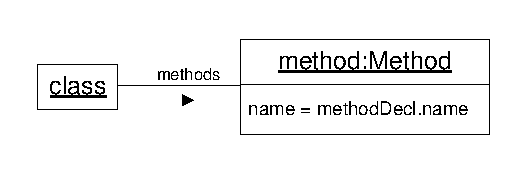
\includegraphics[scale=1]{figures/ObjectConstraint}
  \caption{Matching Pattern with an Attribute Constraint}
  \label{fig:objectConstraint}
\end{figure}

In the example, we match a method being contained in the class represented by the object variable \fe{theClass}. 
The match is restricted to a method which has the name "getName".

The values of attributes that are not restricted by an attribute constraint are not considered during the matching. 
Thus, they may have an arbitrary value. 
In the current version of story patterns, attribute constraints need to be specified using OCL~\cite{OCL}. 
Besides equality checks, all comparative operations on the attributes of an object supported by OCL can be used as object constraints. 

Besides attribute constraints, \emph{attribute assignments} can be used to change the value of an attribute during the application of a story pattern. 
Thus, attribute assignments are considered to be part of the RHS. 
When using attribute assignments, the value of the attribute is not considered while matching the LHS to the instance model. 
Figure \ref{fig:attributeAssignment} shows an example.

\begin{figure}[htbp]
  \centering
  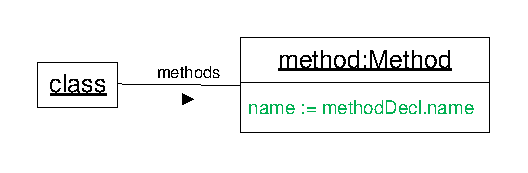
\includegraphics[scale=1]{figures/AttributeAssignment}
  \caption{Using an Attribute Assignment}
  \label{fig:attributeAssignment}
\end{figure}

In the example, the story pattern matches a method with an arbitrary name in the class \fe{theClass}. 
Then, the name of the method is changed to \emph{"getMethodName"}. 

The concrete syntax of an attribute assignment is
\begin{lstlisting}
 <attributeAssignment> ::= #Attribute.name ':=' Expression
\end{lstlisting}
The expression is to be specified using OCL. 
The type of the return value of the OCL expression must be assignable to the type of the attribute. 
Since the attribute value is changed as part of the RHS, the assignment is visualized in green color.

Story patterns also enable to use both, an attribute constraint and an attributed assignment for the same attribute inside one object variable. Then, the attribute constraint is used during the matching step. The attribute value of the object matched to the corresponding object variable is then changed as specified by the attribute assignment while enforcing the RHS.

\begin{figure}[htbp]
  \centering
  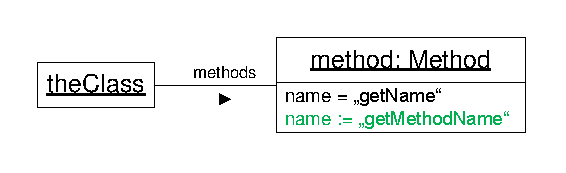
\includegraphics[scale=1]{figures/AttributeConstraintAndAssignment}
  \caption{Using an Attribute Constraint and an Attribute Assignment on the Same Attribute}
  \label{fig:attributeConstraintAndAssignment}
\end{figure}

Figure~\ref{fig:attributeConstraintAndAssignment} combines the story patterns of Figure~\ref{fig:objectConstraint} and~\ref{fig:attributeAssignment}. The story pattern matches an object of type \fe{Method} which has the name \fe{getName}. If the matching was successful, the name of the object bound to \fe{method} is set to \fe{getMethodName} as defined by the attribute assignment.

The OCL statements we allow for attribute constraints and attribute assignments must not traverse the references of the object variables.
Both may only use the attributes of object variables in the same story pattern and arbitrary arithmetic, comparing, and logical operations on them. 





%\ext  %--- Comment this line to include object sets into the document
{
\subsection{Collection Variables}
\label{sec:StoryPatterns:collectionvariables}

Collection variables are special cases of object variables.
They represent an arbitrary number of objects in an instance model that are of the same type.
Thus, a collection variable has the type of the objects within the collection\footnote{We do not
explicitly model collection objects in story diagrams. The type of a collection variable is that of the contained objects and not the type of a collection object like 
\texttt{java.util.Collection}}.

Figure~\ref{fig:CollectionVariableExample} depicts an example story pattern that
contains a collection variable \fe{methods}. During the matching, all
methods in the class that is bound to the object variable \fe{myClass} are
bound to the collection variable \fe{methods}.

\begin{figure}[htb]
  \centering
  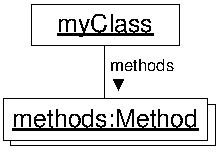
\includegraphics[scale=0.9]{figures/CollectionVariableExample}
  \caption{Collection Variable Example}
  \label{fig:CollectionVariableExample}
\end{figure}

The elements in collection variables are always ordered.
Collections can be specified to only contain unique elements or to allow the same element to be contained multiple times.
This leads to two different types of collections: ordered sets and lists.
Their semantics are similar to collection types in OCL: Elements in
ordered sets are ordered and unique. Elements in a list are ordered, but not necessarily
unique.

Figure~\ref{fig:CollectionVariableTypes} depicts the concrete syntax of the two collection types.

\begin{figure}[htb]
  \centering
  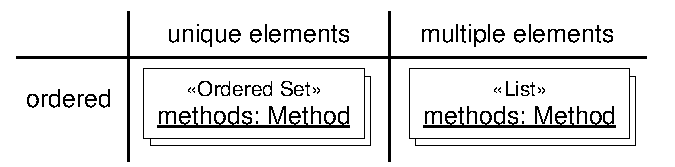
\includegraphics[scale=0.8]{figures/CollectionVariables}
  \caption{Types of collection variables: Ordered Set and List}
  \label{fig:CollectionVariableTypes}
\end{figure}


Two matched collection variables in the same story pattern do not have to be disjoint.
Thus, isomorphism is not enforced for the content of two or more collection variables.
Link variables between two collection variables are not allowed.

An attribute determines if the collection represented by a collection variable can be empty. 
If this is the case, a collection variables is considered to be optional in a
matching. Additionally, object constraints can be used to specify the allowed size of
the collection using OCL.

As the matching of collection variables is implicitly optional, their binding semantics cannot be set to ``optional'', explicitly.
Negative collection variables are not allowed.
Furthermore, collection variables in combination with a \create binding operator
are not allowed: collection variables can only be used in combination with the
binding operators ``check only'' or \destroy.

%\todomcp{explain set size expressions (do we change the name?)}
%\tododt{We should call the formerly known ObjectSetSizeExpression simply
%CollectionSizeExpression.}
%\todomvd{According to the meeting on May, 25th, set size expressions are
%omitted in v0.2. We can use OCL instead.}

%\todomcp{If we bind an object set, can we use the bound object in other story
%pattern? E.g., to insert all elements bound by the object set into a container
%via a containment link?}
%\tododt{Yes, but I would use another concrete syntax (see
%Figures~\ref{fig:reuseObjSet1}, \ref{fig:InclusionLinksExample1}).}

%\begin{figure}[htb]
%		\centering
%		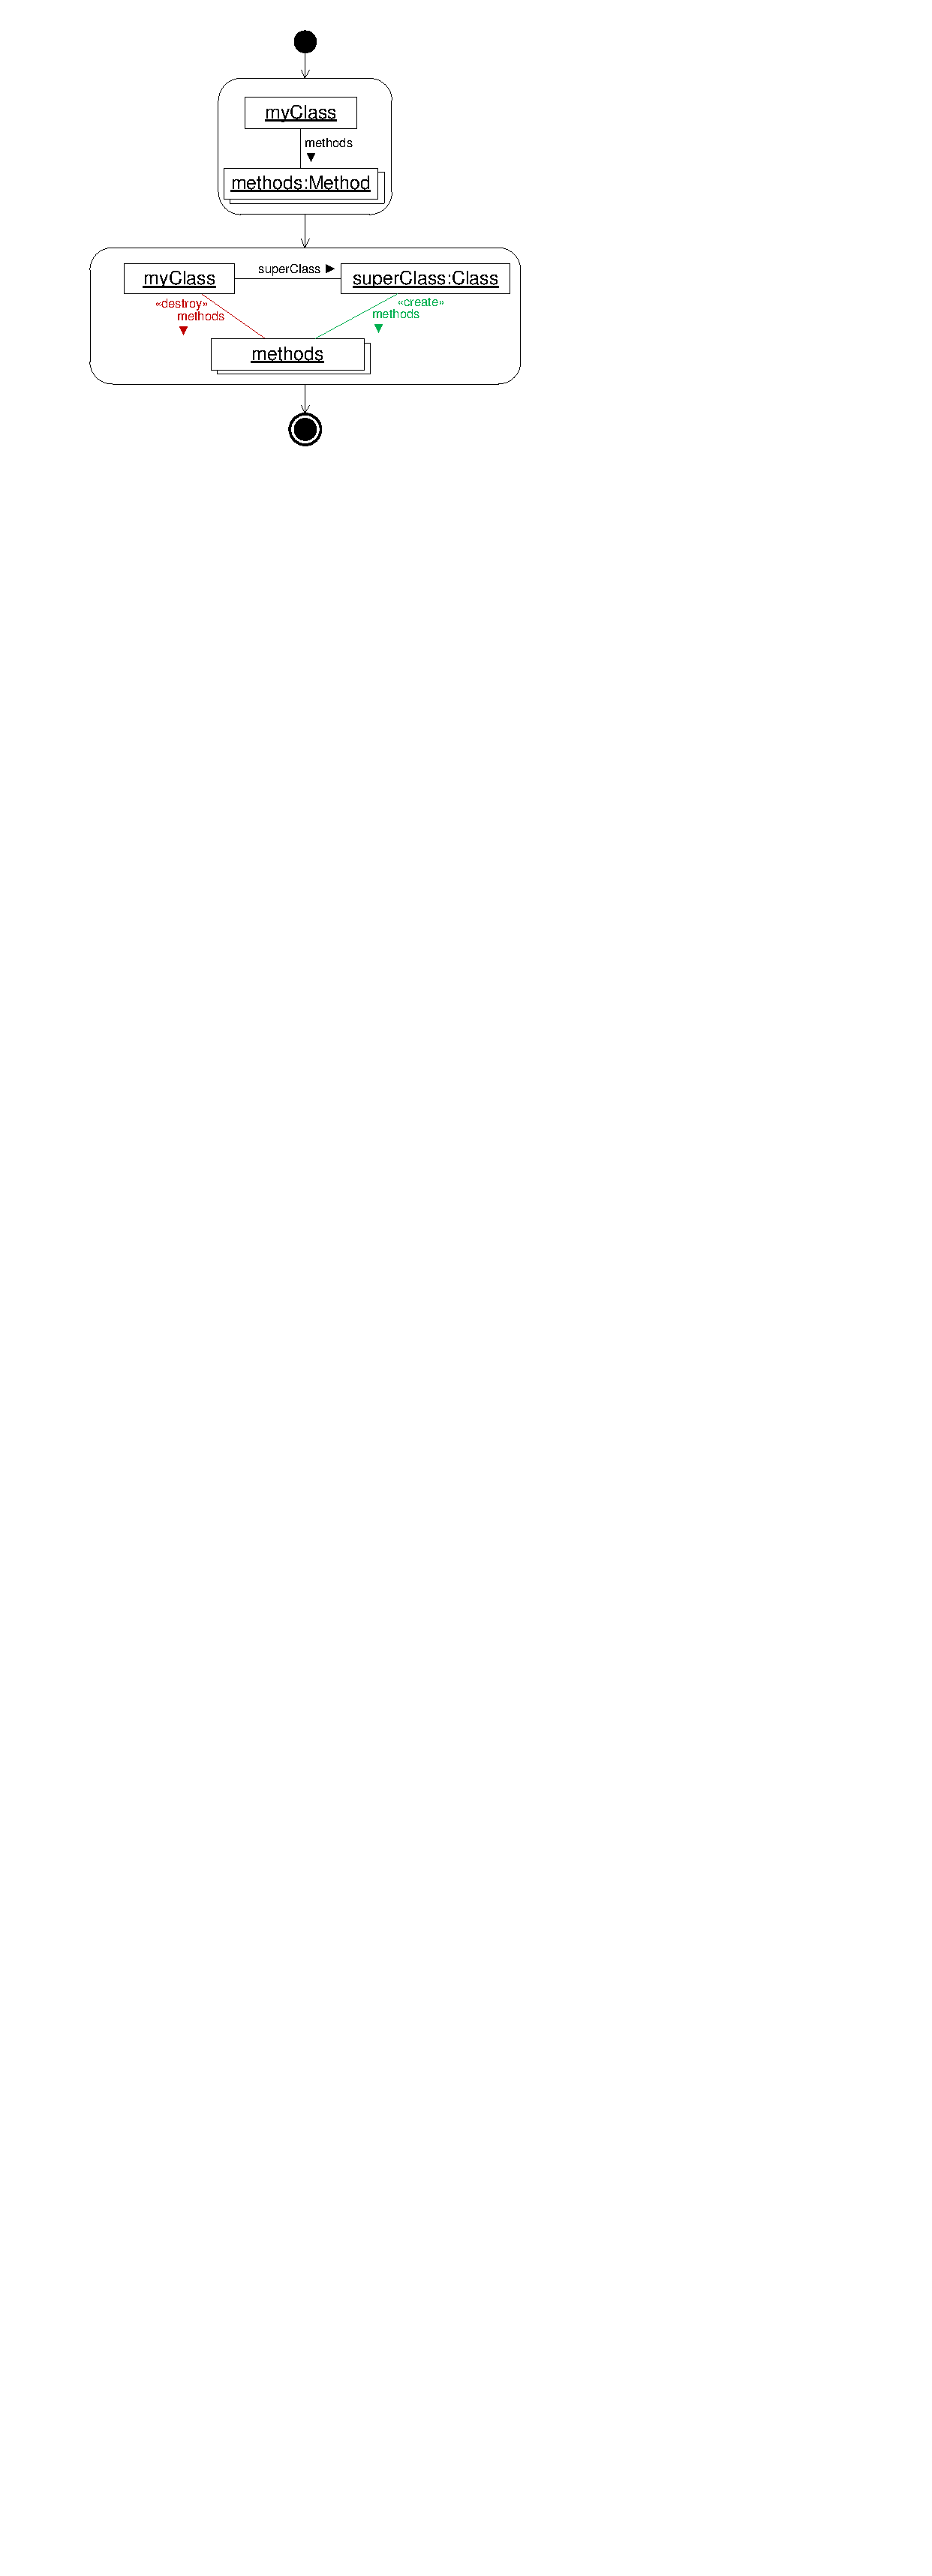
\includegraphics[scale=.8]{figures/ReuseObjectSet1}
%  	\caption{Reuse Objects in a Set}
%  	\label{fig:reuseObjSet1}
%\end{figure} 

%\todomcp{A collection variable contains no ObjectSetSizeExpression and no
%object is matched into the object set: collection variable is interpreted as
%optional and the matching succeeds.} 
%\tododt{We still should add an attribute to \fe{CollectionVariable} to
%distinguish the cases where at least one object should be matched or any number
%of objects including zero should be matched. Stephan also wanted this
%expressiveness.}


}%------ End of collection variable section


\subsection{Inclusion Links}
\label{sec:StoryPatterns:inclusion}

There are cases when you want to add additional objects to a set of objects matched to a collection variable
as described in Section~\ref{sec:StoryPatterns:collectionvariables}.
For example, when collecting all methods in a class hierarchy that comply to a certain method signature,
you would go through all classes in the hierarchy and add complying methods step by step.
Since a collection variable does not explicitly represent a collection object in
the sense of Java (as described in Section~\ref{sec:StoryPatterns:collectionvariables},
we need a way to describe the addition or removal ofobjects to or from such an object collection
as well as checking if an object is included in an object collection.
We introduce \emph{inclusion links} for this purpose.

\begin{figure}[htb]
	\begin{minipage}{.43\textwidth}
		\centering
		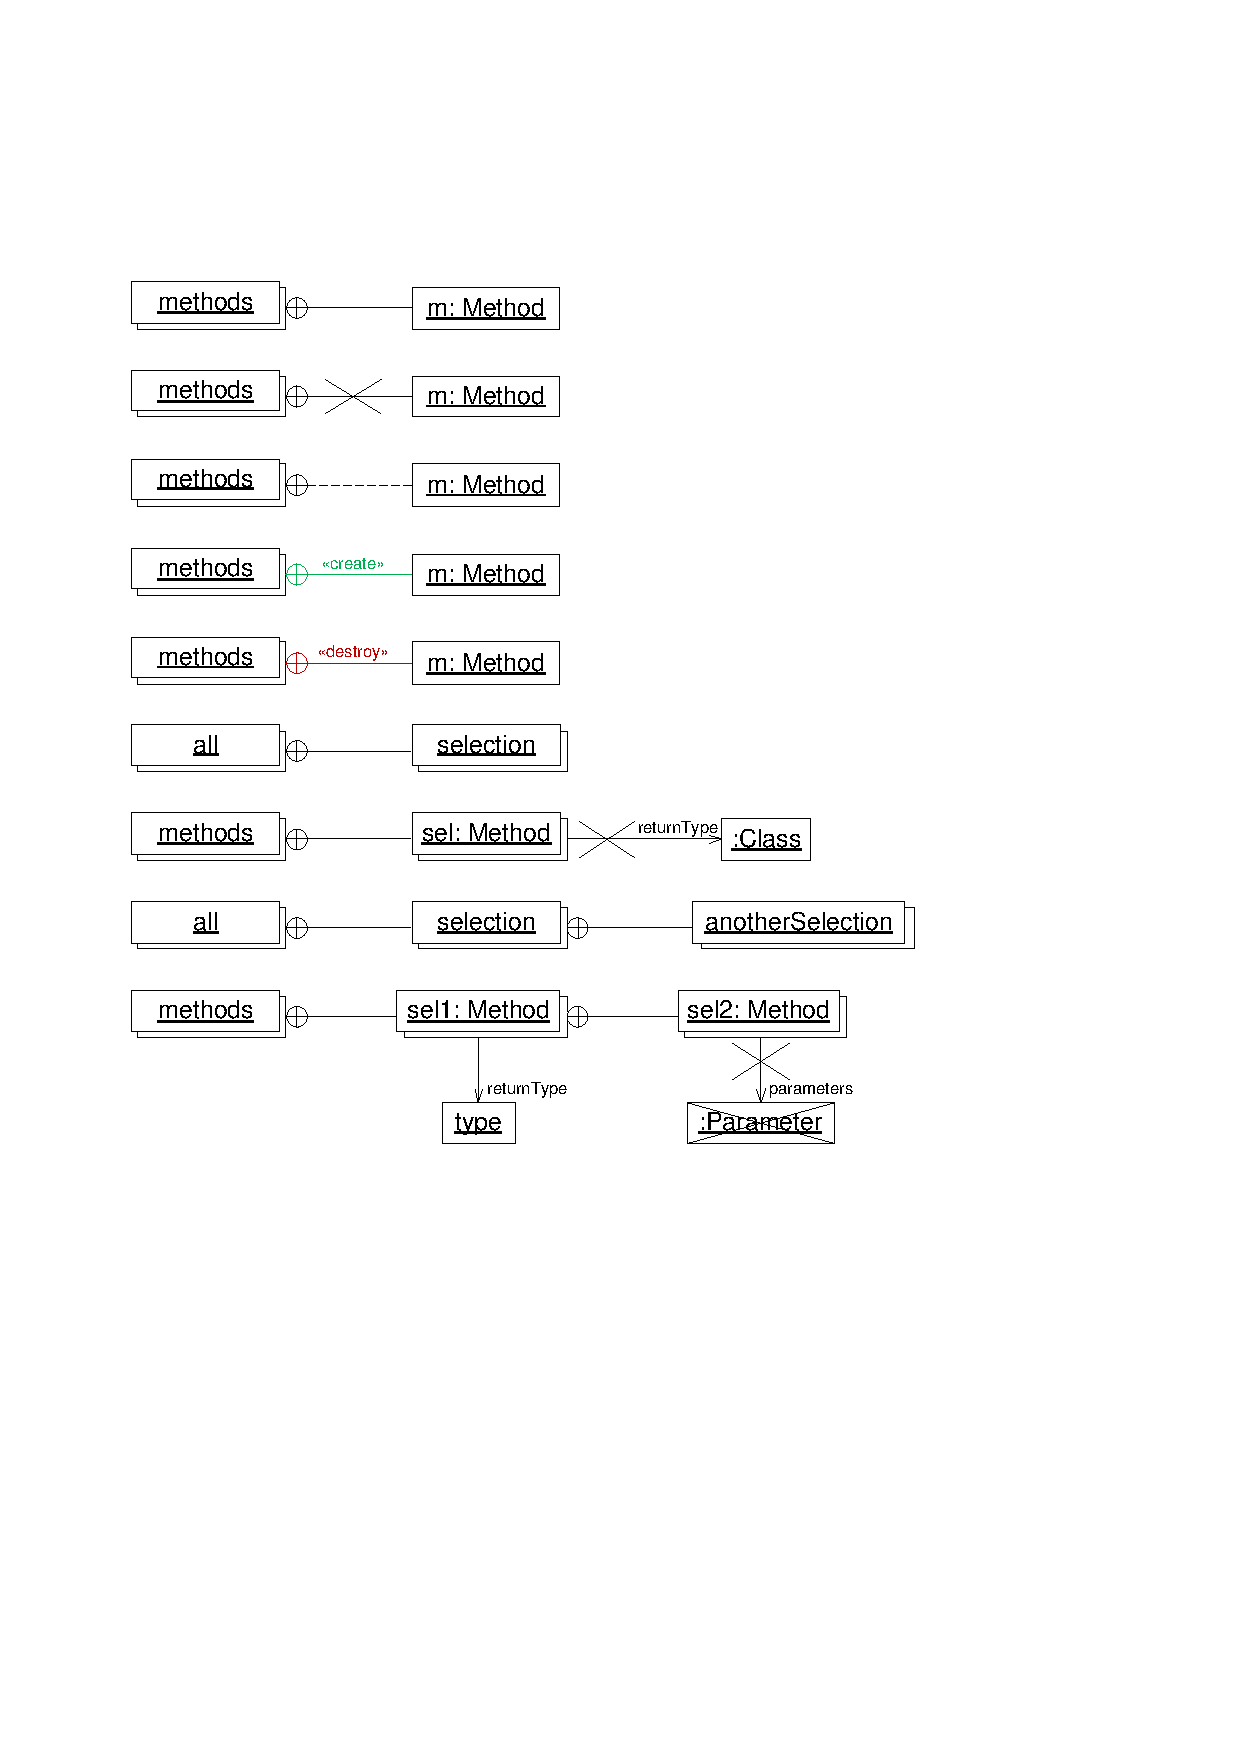
\includegraphics[width=\linewidth]{figures/InclusionLinks}
    \caption{Notation of Inclusion Links}
    \label{fig:InlucionLinks}
	\end{minipage}
  \hfill
  \begin{minipage}{.47\textwidth}
  	\centering
		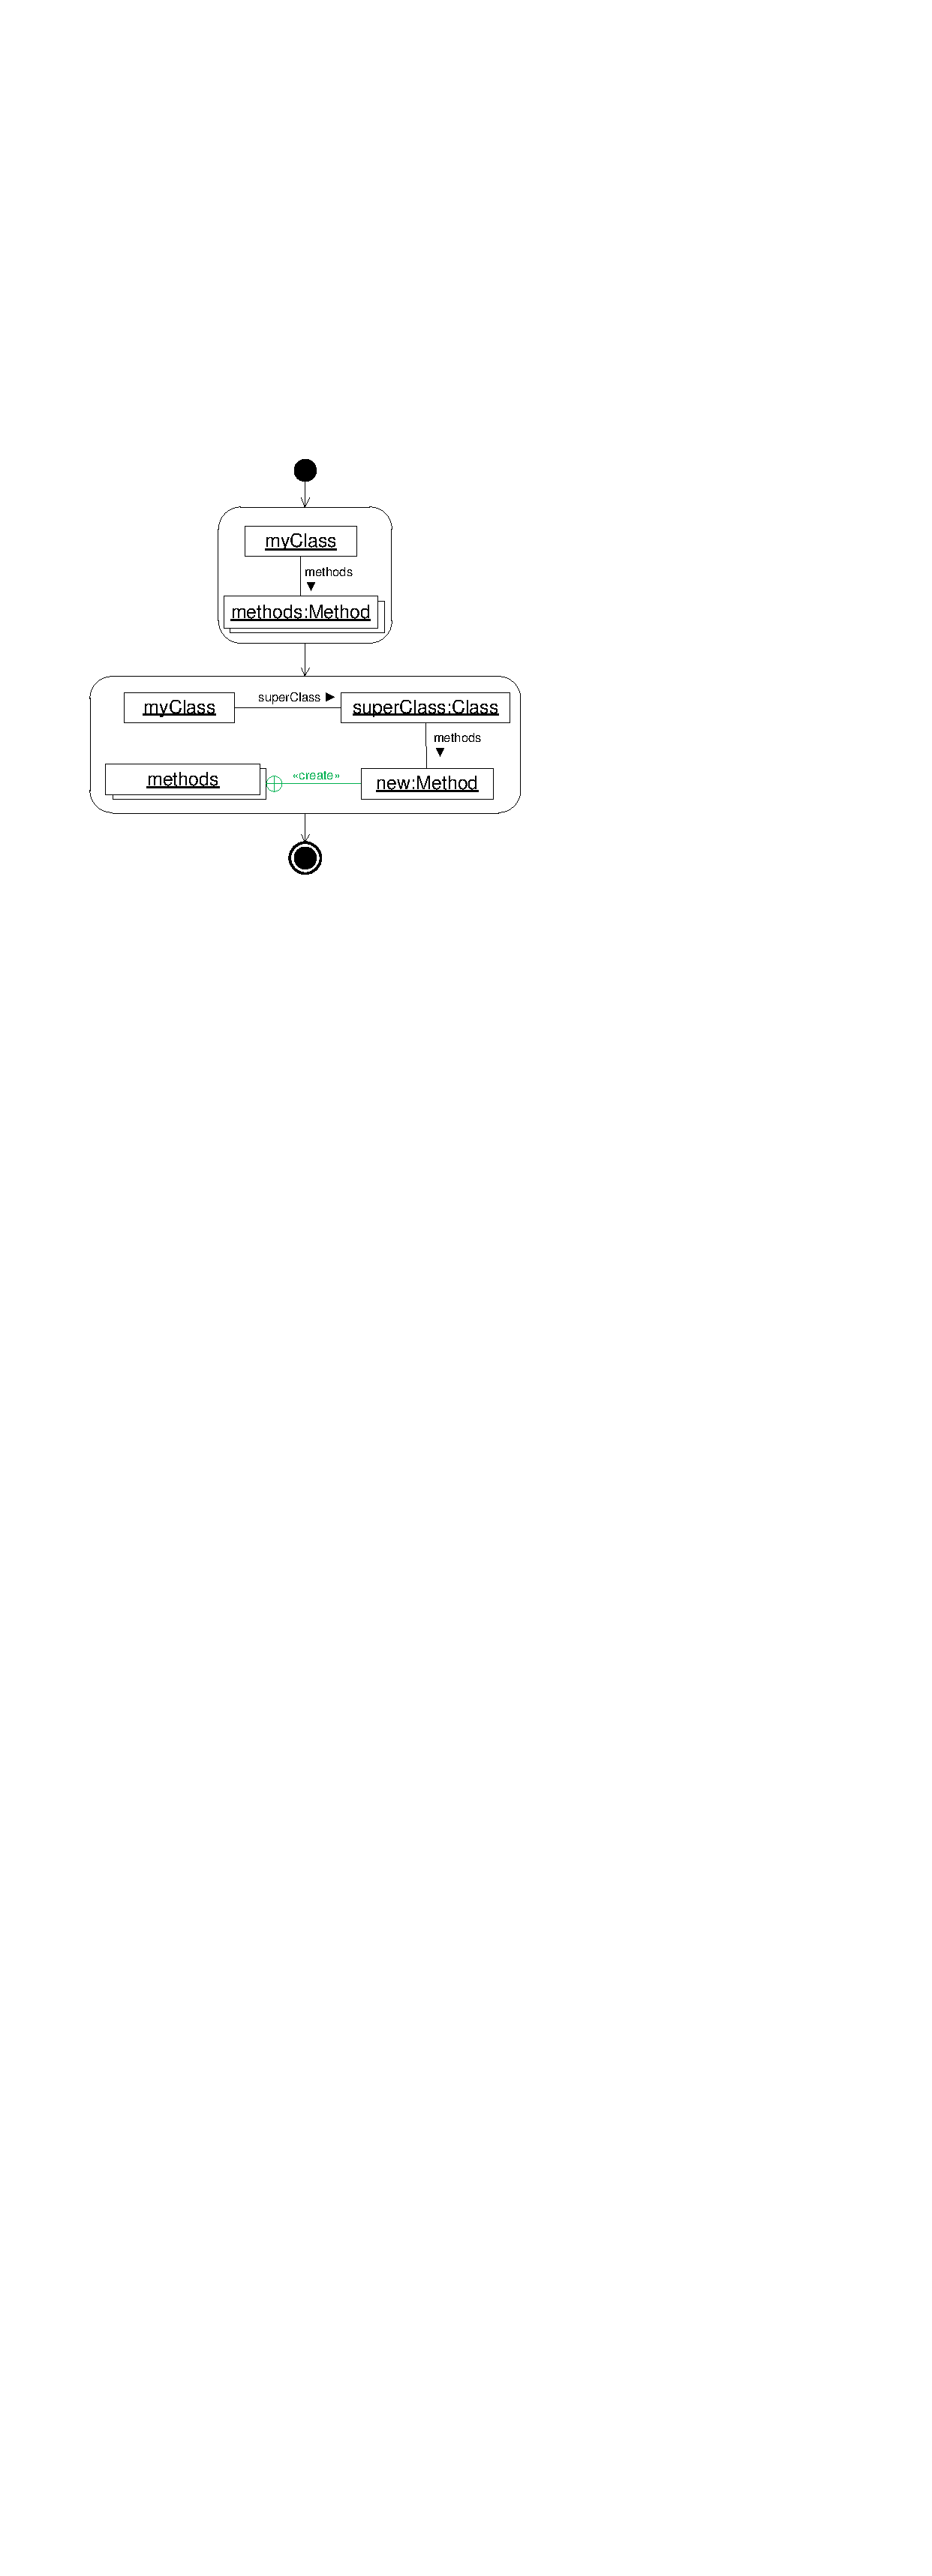
\includegraphics[width=\linewidth]{figures/InclusionLinksExample1}
    \caption{Add an Object to a Collection}
    \label{fig:InclusionLinksExample1}
	\end{minipage}
\end{figure}

An inclusion link represents a containment relation between two variables in a story pattern.
It can be used between a collection variable and another variable to specify that
an object (or a set of objects) represented by a variable is contained in an object set represented by a collection variable.
An inclusion link is represented by a line between a collection variable and another object
variable as illustrated in Figure~\ref{fig:InlucionLinks}~a).
The circle containing a plus determines which of the two sides of the link is containing the other one.
In Figure~\ref{fig:InlucionLinks}~a), the collection \fe{methods} contains an object \fe{aMethod}.

In contrast to link variables that are typed over an association,
\tododt{In fact, these are one or two references.}
inclusion links are not typed at all.
They only represent a containment of an object in a collection of objects.
But similar to link variables, this relation can be checked to be existent between a collection and an object
or be used to match new objects.
While the pattern in Figure~\ref{fig:InlucionLinks} a) specifies to check if the object \fe{aMethod} is contained in the collection \fe{methods},
the pattern in Figure~\ref{fig:InlucionLinks} b) specifies to match a \fe{Method} object which is contained in the collection \fe{methods}.

Similar to other links, inclusion links can be used with object variables that are bound, unbound, or maybe-bound.
Inclusion links can also be negative or optional and can be combined with \create\ or \destroy\ stereotypes (see Figure~\ref{fig:InlucionLinks} a) to f)).
Case c) in Figure~\ref{fig:InlucionLinks} defines that the matching is only successful if no \fe{Method} object can be found in the \fe{methods} collection.
Accordingly, case d) specifies to optionally match a \fe{Method} object contained in the \fe{methods} collection
(see the description of binding semantics in Section~\ref{sec:StoryPatterns:binding:semantics} for details).
Case e) specifies to create an inclusion relation between the object \fe{aMethod} and the collection \fe{methods},
i.e., to add the object \fe{aMethod} to the collection \fe{methods}.
Analogously, case f) specifies to remove the object \fe{aMethod} from the collection \fe{methods}.
Furthermore, inclusion links can also be used between two collection variables as illustrated in Figure~\ref{fig:InlucionLinks} f)
to check if all objects in the collection \fe{selection} are contained in the collection \fe{all}.

By means of inclusion links, a collection variable that has been matched to a set of objects
can be modified afterwards by adding or removing objects.
Using story diagrams as described in Section~\ref{sec:StoryDiagrams},
one can, for example, collect a set of \fe{Method} objects in a collection \fe{methods}
as illustrated in the first story node in Figure~\ref{fig:InclusionLinksExample1}
and then add another \fe{Method} object to the same collection in a following story node that reuses the previously matched set of objects.

\begin{figure}[htb]
  \centering
  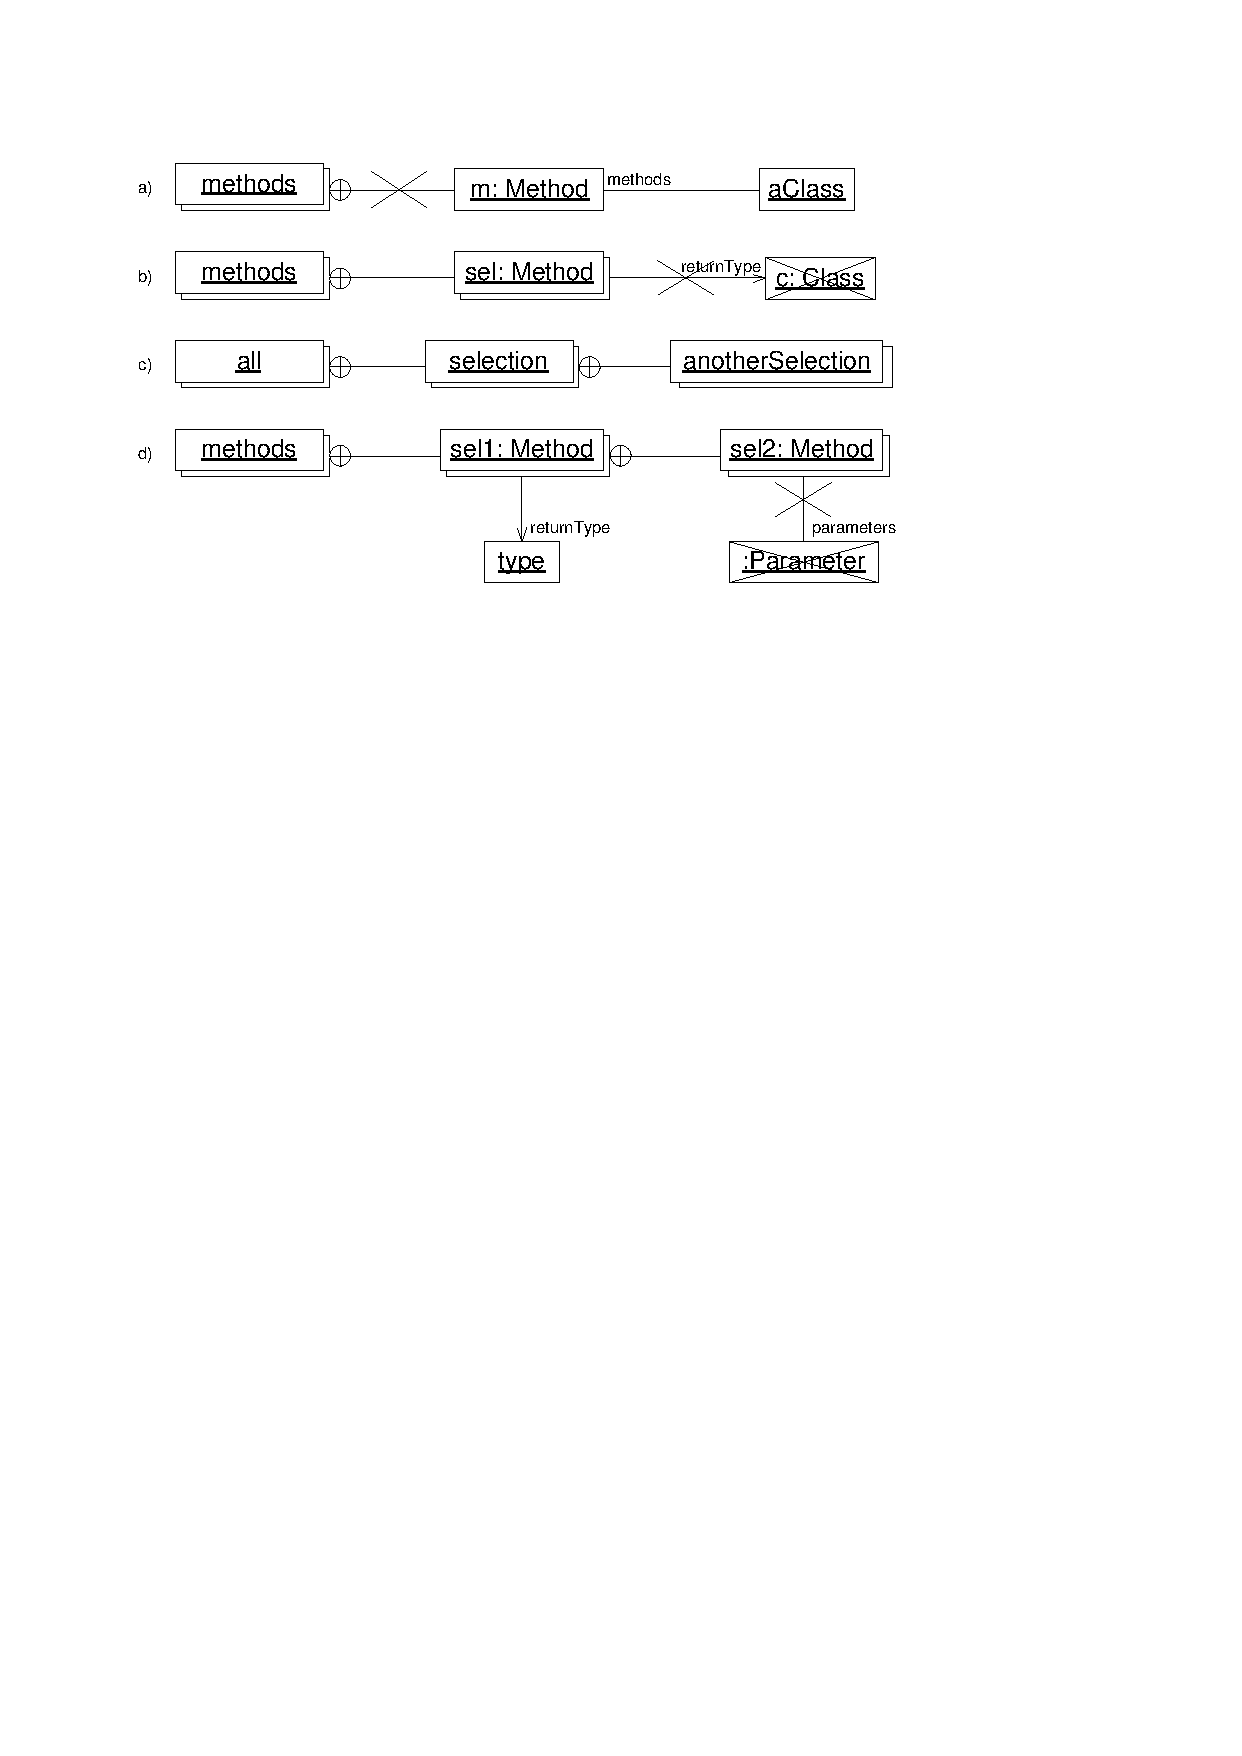
\includegraphics[scale=0.8]{figures/InclusionLinksExamples}
  \caption{Exemplary Uses of Inclusion Links}
  \label{fig:InlucionLinksExamples}
\end{figure}

Inclusion links can be used in combination with link variables.
In Figure~\ref{fig:InlucionLinksExamples} we give some examples for possible uses.
In case a) the story pattern specifies that a \fe{Method} object is to be found which is defined in a class \fe{aClass},
but which is not contained in the collection \fe{methods}.
Case b) specifies to find a collection \fe{sel} of \fe{Method} objects which are contained in the collection \fe{methods}
and do not have a return type that is a \fe{Class} object.
The pattern in case c) checks whether a set of objects described by the collection \fe{all} contains another set of objects described by the collection \fe{selection}
which in turn contains another set of objects described by the collection \fe{anotherSelection},
i.e., \fe{anotherSelection} is a subset of \fe{selection} and \fe{selection} is a subset of \fe{all}.
The pattern in case d) specifies to find two object sets that are subsets of another set.
First, a collection \fe{sel1} of \fe{Method} objects which have the return type \fe{type} is to be found in the collection \fe{methods}.
Second, a collection \fe{sel2} of \fe{Method} objects which additionaly have no parameters is to be found in the collection \fe{sel1}.


\subsubsection{Feasible Uses of Inclusion Links}
\label{sec:StoryPatterns:inclusion:feasible}

Inclusion links can be used exactly like link variables except that the source of an inclusion link has to be a collection variable.

Inclusion links can be used with all available binding semantics as described in Section~\ref{sec:StoryPatterns:binding:semantics}.
Consequently, if you replace a negative or optional link variable in Figures~\ref{fig:negativeObjects} and \ref{fig:optionalObjects}
with a negative or optional inclusion link
(independent of the inclusion link's direction and assuming that an inlucion link's source is a collection variable),
you get the feasible combinations of binding semantics used with inclusion links.

Moreover, you get all feasible combinations of binding operators and inclusion links from
Table~\ref{tab:bindingCombinations_links} in Section~\ref{sec:StoryPatterns:binding:operators}.

\begin{figure}[htbp]
  \centering
  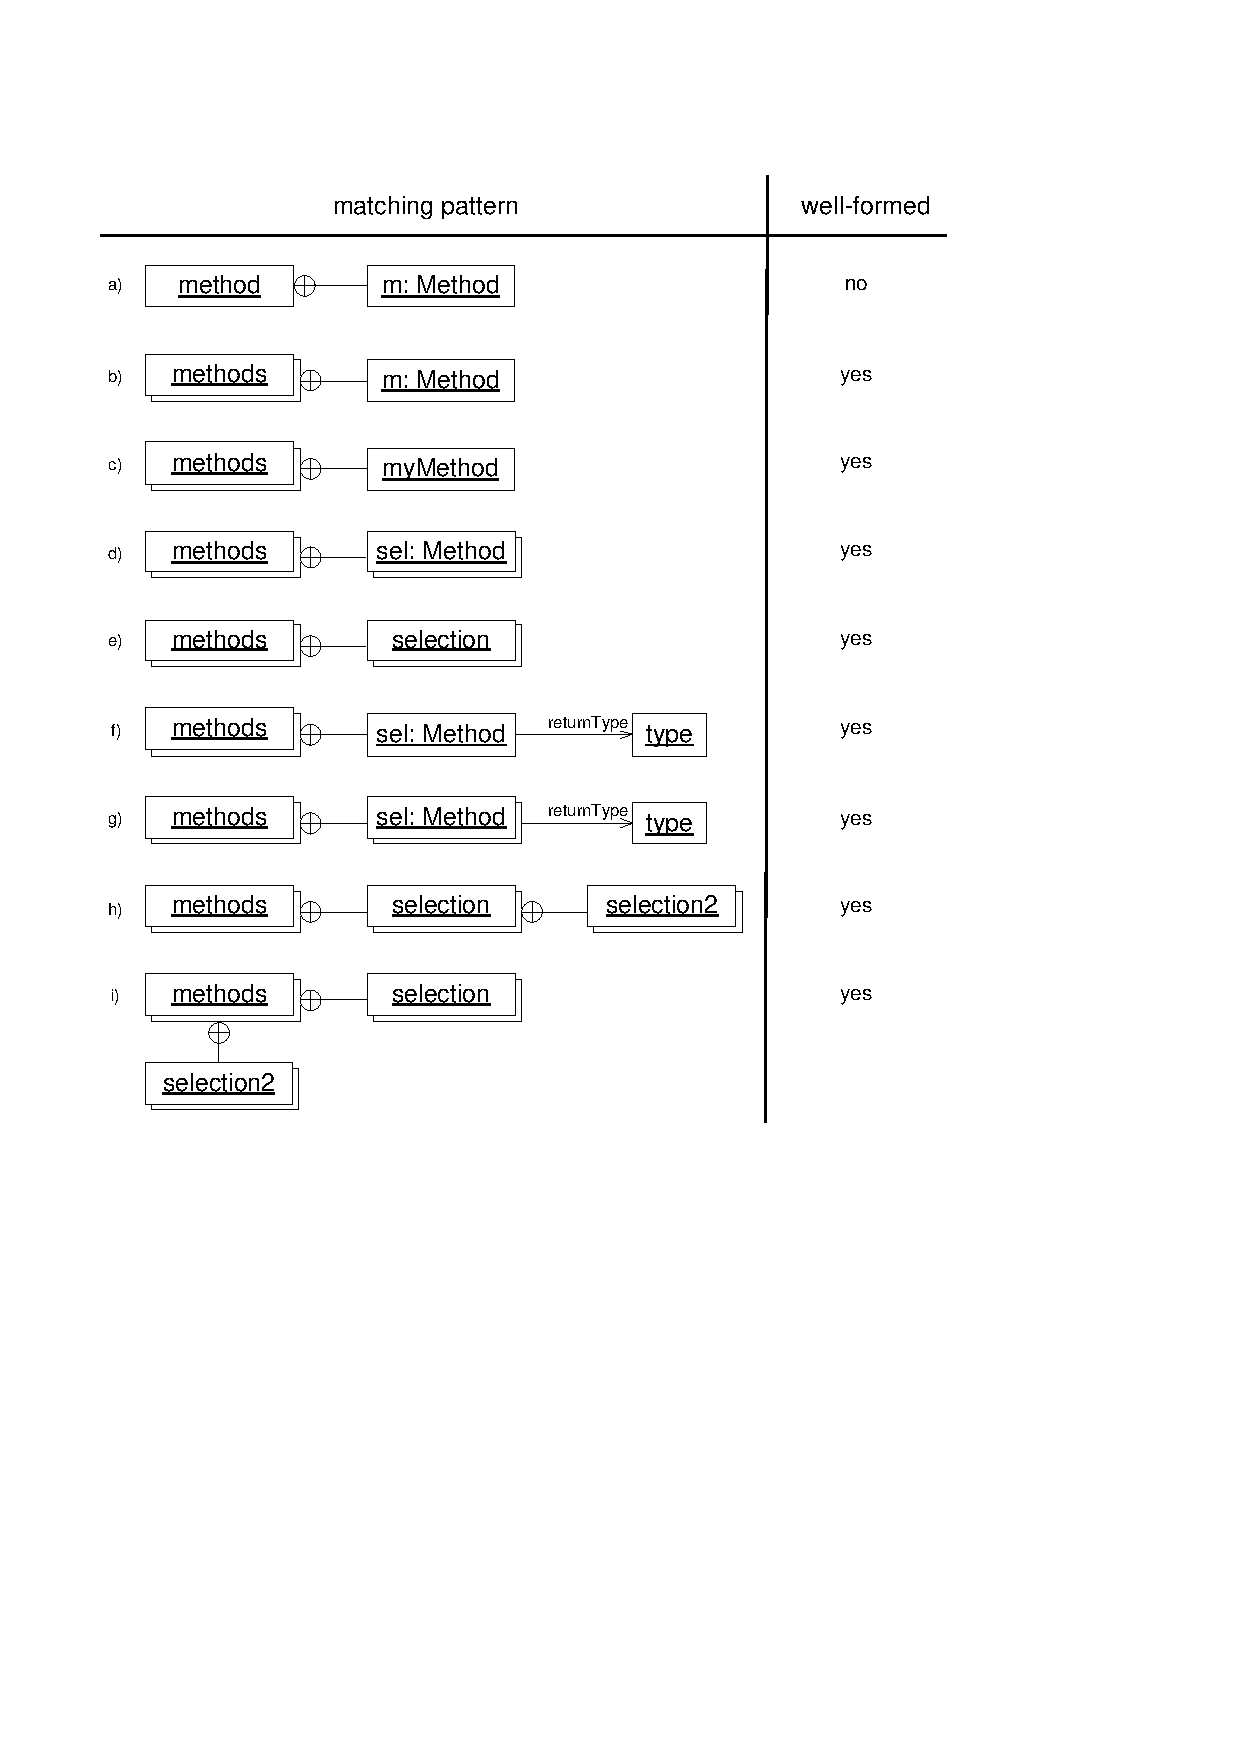
\includegraphics[scale=0.8]{figures/InclusionLinksWellFormedness}
  \caption{Well-formedness of inclusion links}
  \label{fig:InlucionLinkWellFormedness}
\end{figure}

In addition, different combinations of collection variables connected to a bound or unbound variable and
to a single object variable or a collection variable are feasible as illustrated in Figure~\ref{fig:InlucionLinkWellFormedness}.


\subsubsection{Collection Operations with Inclusion Links}
\label{sec:StoryPatterns:inclusion:BagsSetsEtc}

Inclusion links cannot only be used between a collection variable and a single object variable
as shown in Figure~\ref{fig:InlucionLinks} (p.~\pageref{fig:InlucionLinks}),
but also between two collection variables as shown in Figure~\ref{fig:InlucionLinkCollections}.
The semantics for this case are explained in the following.

\begin{figure}[htb]
  \centering
  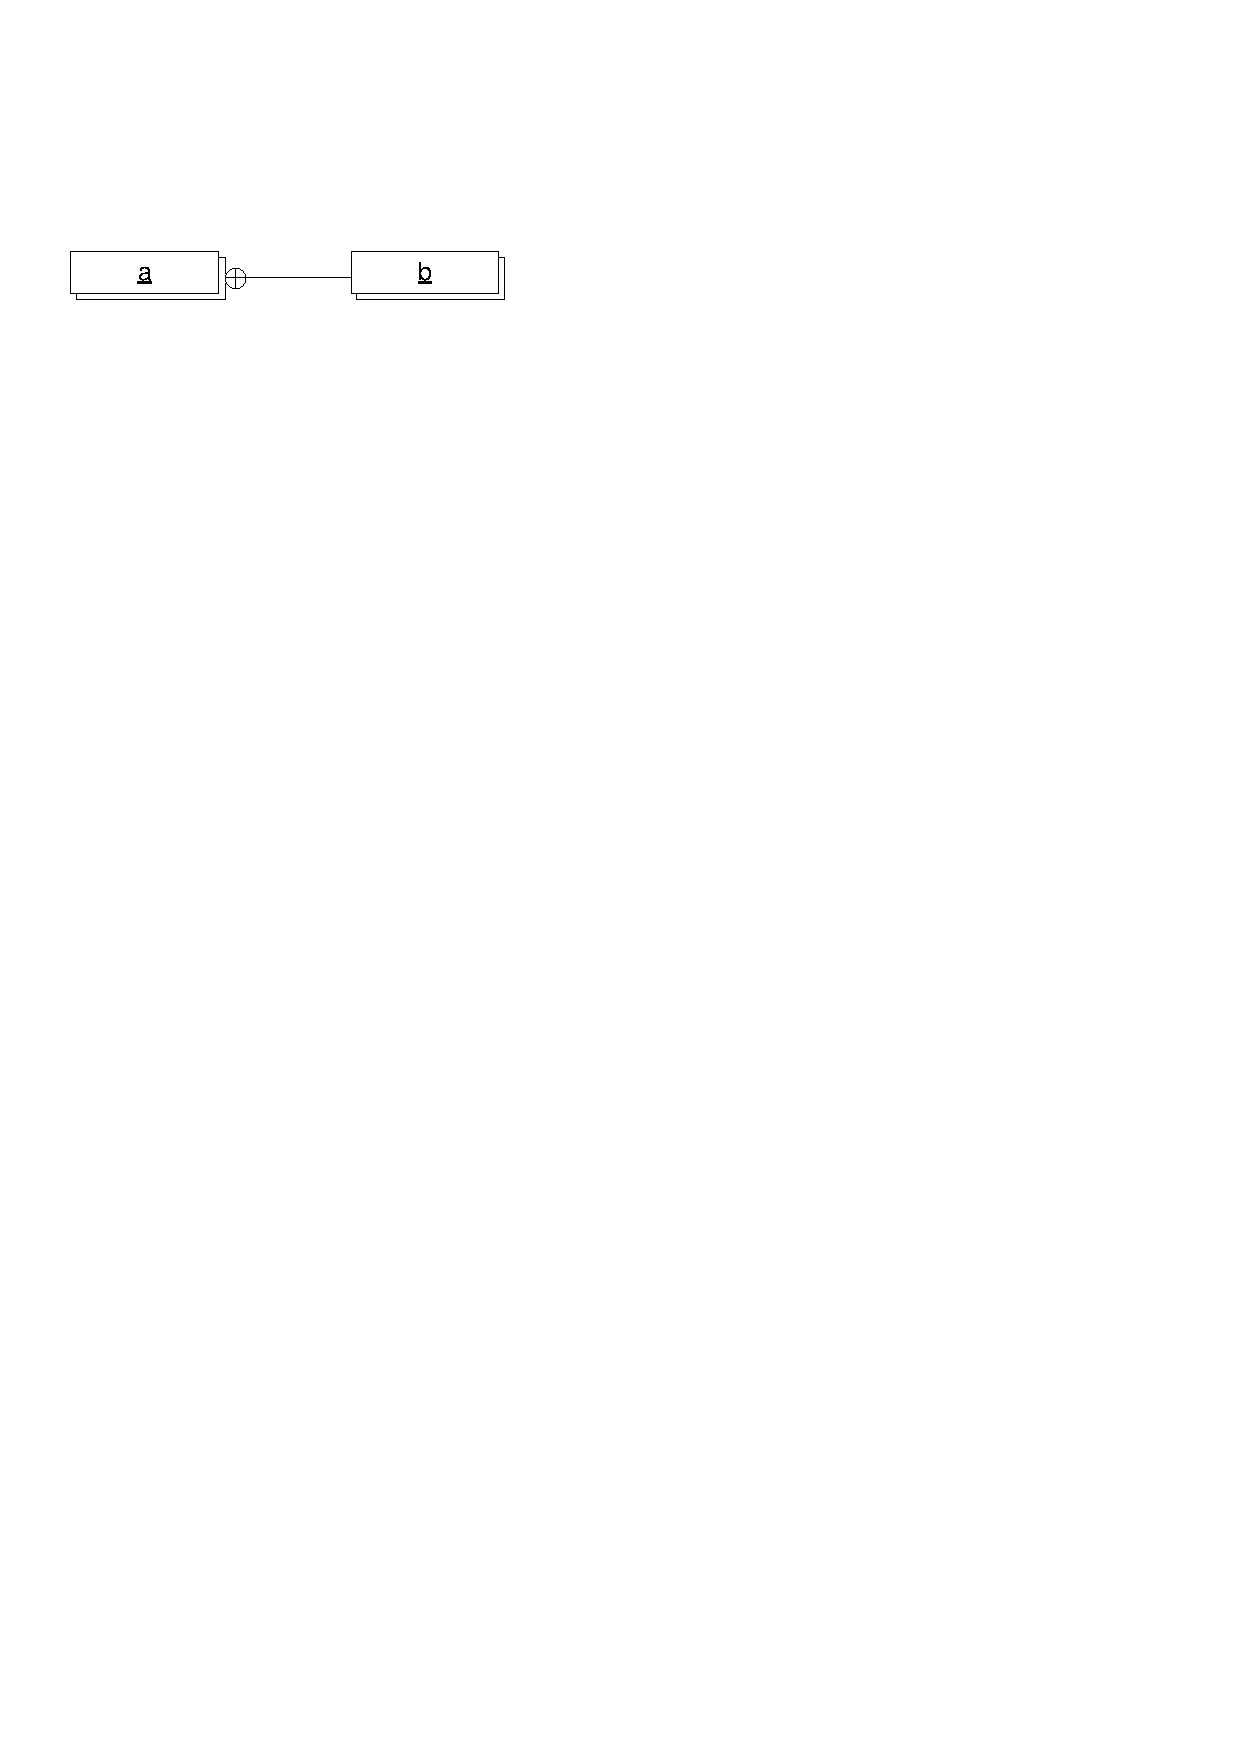
\includegraphics[scale=0.8]{figures/InclusionLinksSetsCheck}
  \caption{Inclusion Link Between Two Collections}
  \label{fig:InlucionLinkCollections}
\end{figure}

An inclusion link between two collection variables represents a containment relation between two sets of objects, i.e., between two collections.
In case of the illustration in Figure~\ref{fig:InlucionLinkCollections},
the collection \fe{b} depicts a subset of the set represented by the collection \fe{a} (mathematically $b \subseteq a$).
Interpreting the Figure~\ref{fig:InlucionLinkCollections} as a story pattern,
it describes to check if the elements in collection \fe{b} are also contained in the collection \fe{a}.

In Section~\ref{sec:StoryPatterns:collectionvariables} we introduced different types of collection variables.
We distinguish between ordered sets and lists.
Sets contain an element mostly once (\emph{unique} property) while lists can contain an element arbitrarily often.
Consequently, the inclusion links between different types of collection variables have different semantics,
which are described in Table~\ref{tab:set_operations_with_inclusion_links}.
The first two columns determine the type of the collections \fe{a} and \fe{b}.
The third column determines if the inclusion link is to be checked, created or removed.
The last column describes the semantics.

The main difference in the semantics of inclusion links stems from the unique or non-unique property of the collections.
If \fe{a} is a set and the binding operator is \fe{CHECK\_ONLY}, the execution of a story pattern
only checks if all objects in \fe{b} are contained (once) in \fe{a}
(mathematically $a \supseteq b$).
In contrast, if \fe{a} is a list (which can contain the same object arbitrarily often),
the story pattern execution ensures that the objects in \fe{b} are not only contained at least once in \fe{a},
but also at least as often as in \fe{b}.
If, for example, \fe{b} contains an element \fe{x} twice, then \fe{a} has to contain \fe{x} at least twice, too.
Otherwise, the matching of the story pattern fails.

An inclusion link with the binding operator \create\ describes to add all objects from \fe{b} to \fe{a}.
If \fe{a} is a set, the story pattern execution only adds each object from \fe{b} to \fe{a}
if \fe{a} does not already contain it. %(remember that sets contain each object mostly once).
Since story patterns only have ordered sets, the order of the objects in the collections have to be regarded.
The story pattern execution adds the objects from \fe{b} to the end of \fe{a} and keeps the same order as they had in \fe{b}.
If \fe{a} is a list, a similar adding operation is performed,
the objects from \fe{b} are added as often to \fe{a} as they are in \fe{b}.
This can be seen as a concatenation of two lists or as the union of two sets (mathematically $a \cup b$).

The binding operator \destroy\ used with an inclusion link and two collections as illustrated in Table~\ref{tab:set_operations_with_inclusion_links}
describes to remove all elements contained in \fe{b} from the collection \fe{a}.
If \fe{a} is a set, all occurrences of the objects in \fe{b} are removed from \fe{a} and the order of the remaining elements in \fe{a} is preserved.
If \fe{a} is a list and \fe{b} is a set, quite the same is done.
If an object contained in \fe{b} is contained more than once in \fe{a}, all of its occurrences in \fe{a} are removed.
This comes close to the mathematical relative complement operation (mathematically $a \setminus b$).
If both, \fe{a} and \fe{b} are lists,
only as many occurrences of the objects in \fe{b} are removed from \fe{a} as these are available in \fe{b}.
Furthermore, the removal starts at the beginning of the list \fe{a}.

\begin{table}[htbp]
%  \footnotesize
  \centering
%  \begin{longtable}{|l|l|c|p{4.6cm}|}
  \caption{Inclusion Links Between Two Collection Variables}
  \label{tab:set_operations_with_inclusion_links}
    \begin{tabular}{|l|l|c|p{4.6cm}|}
    \hline
    \textbf{Type of \fe{a}} & \textbf{Type of \fe{b}} & \textbf{Binding Operation} & \textbf{Semantics} \\
    \hline
    \multicolumn{3}{|c}{
      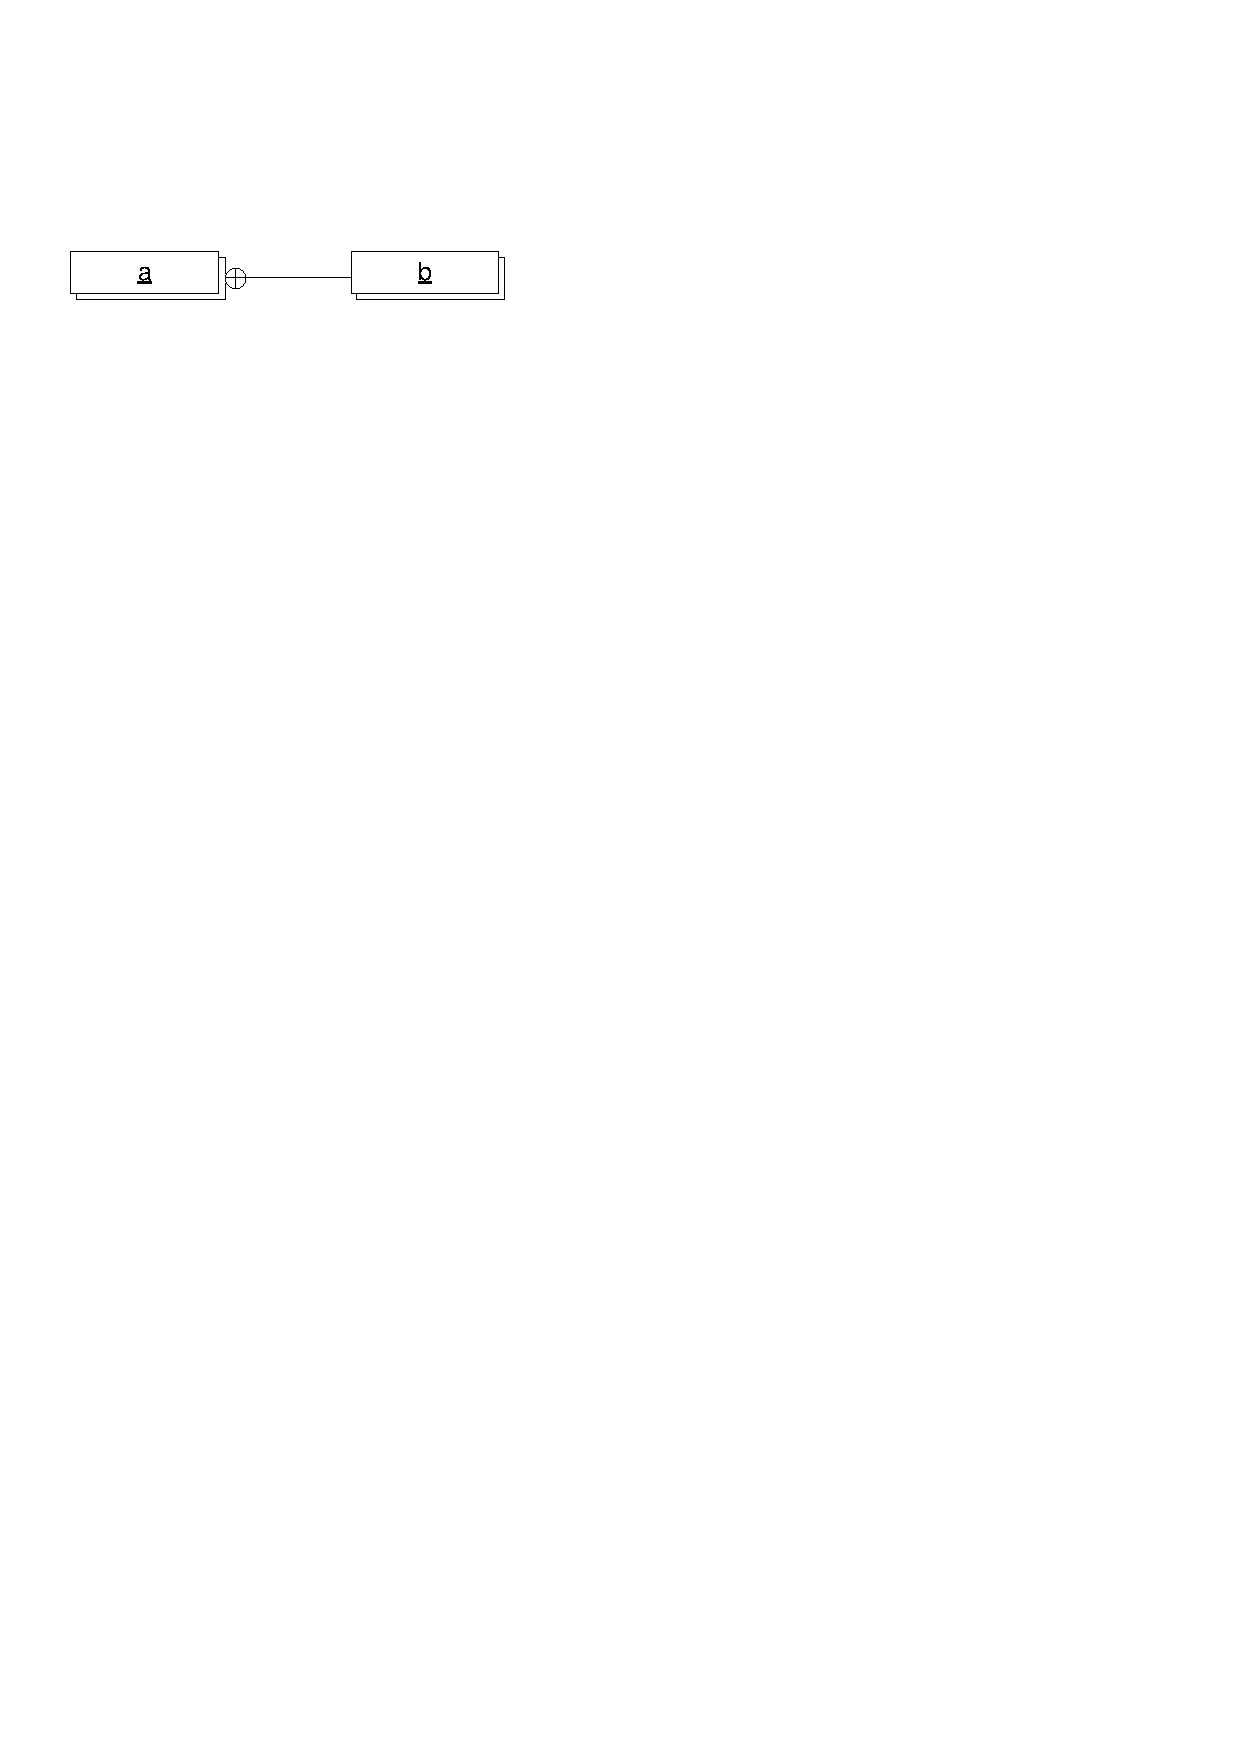
\includegraphics[scale=0.8]{figures/InclusionLinksSetsCheck}
    } & \\
    \hline
    Ordered Set & any & CHECK\_ONLY & Each element in \fe{b} is contained (once) in \fe{a}. \\[0.5em]
    List & any & CHECK\_ONLY & Each element in \fe{b} is contained at least as often in \fe{a} as in \fe{b}.\\
    \hline
    \multicolumn{3}{|c}{
      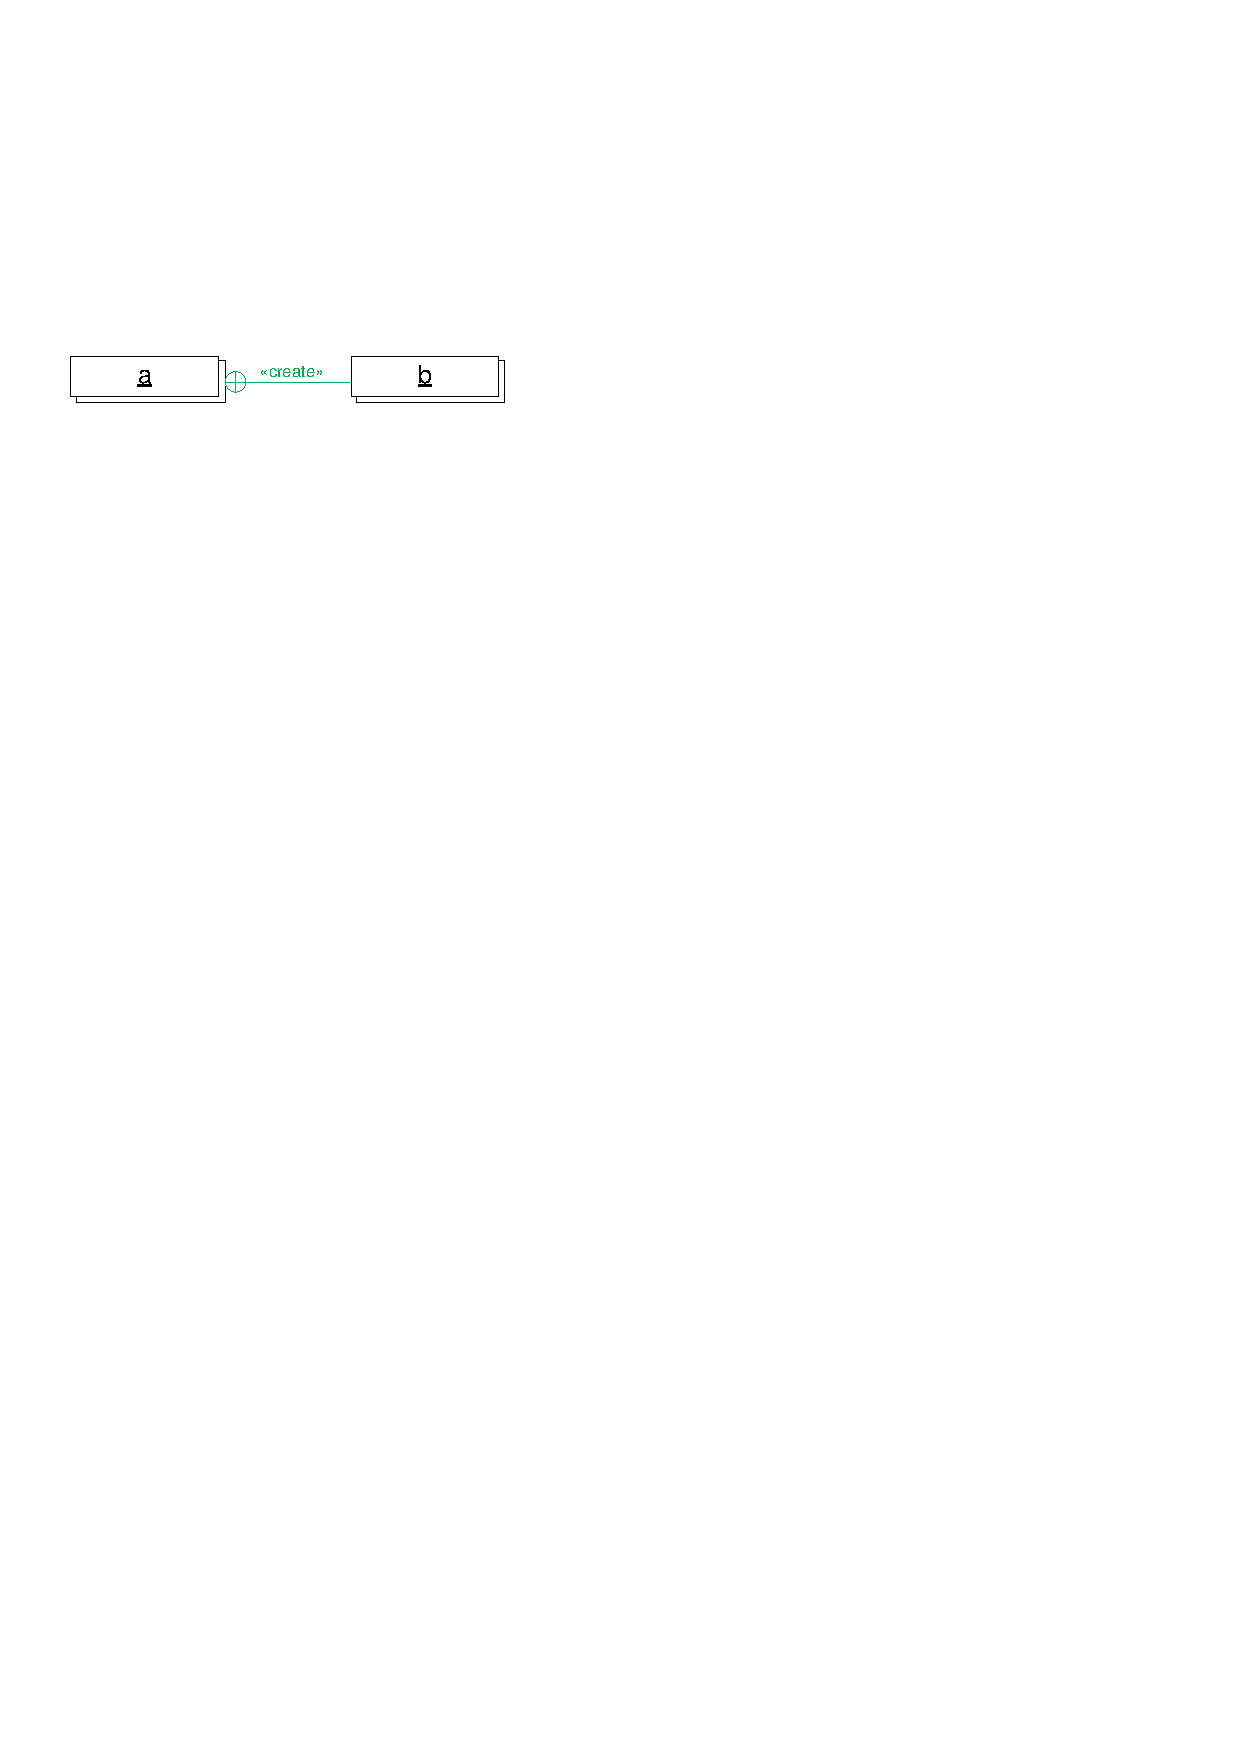
\includegraphics[scale=0.8]{figures/InclusionLinksSetsCreate}
    } & \\
    \hline
    Ordered Set & any & CREATE & Add all elements from \fe{b} to \fe{a} that are missing in \fe{a} to the end of \fe{a}, preserving the order of elements in \fe{b}.\\[0.5em]
    List & any & CREATE & Add all elements from \fe{b} to the end of \fe{a}, preserving the order of elements in \fe{b}.\\
    \hline
    \multicolumn{3}{|c}{
      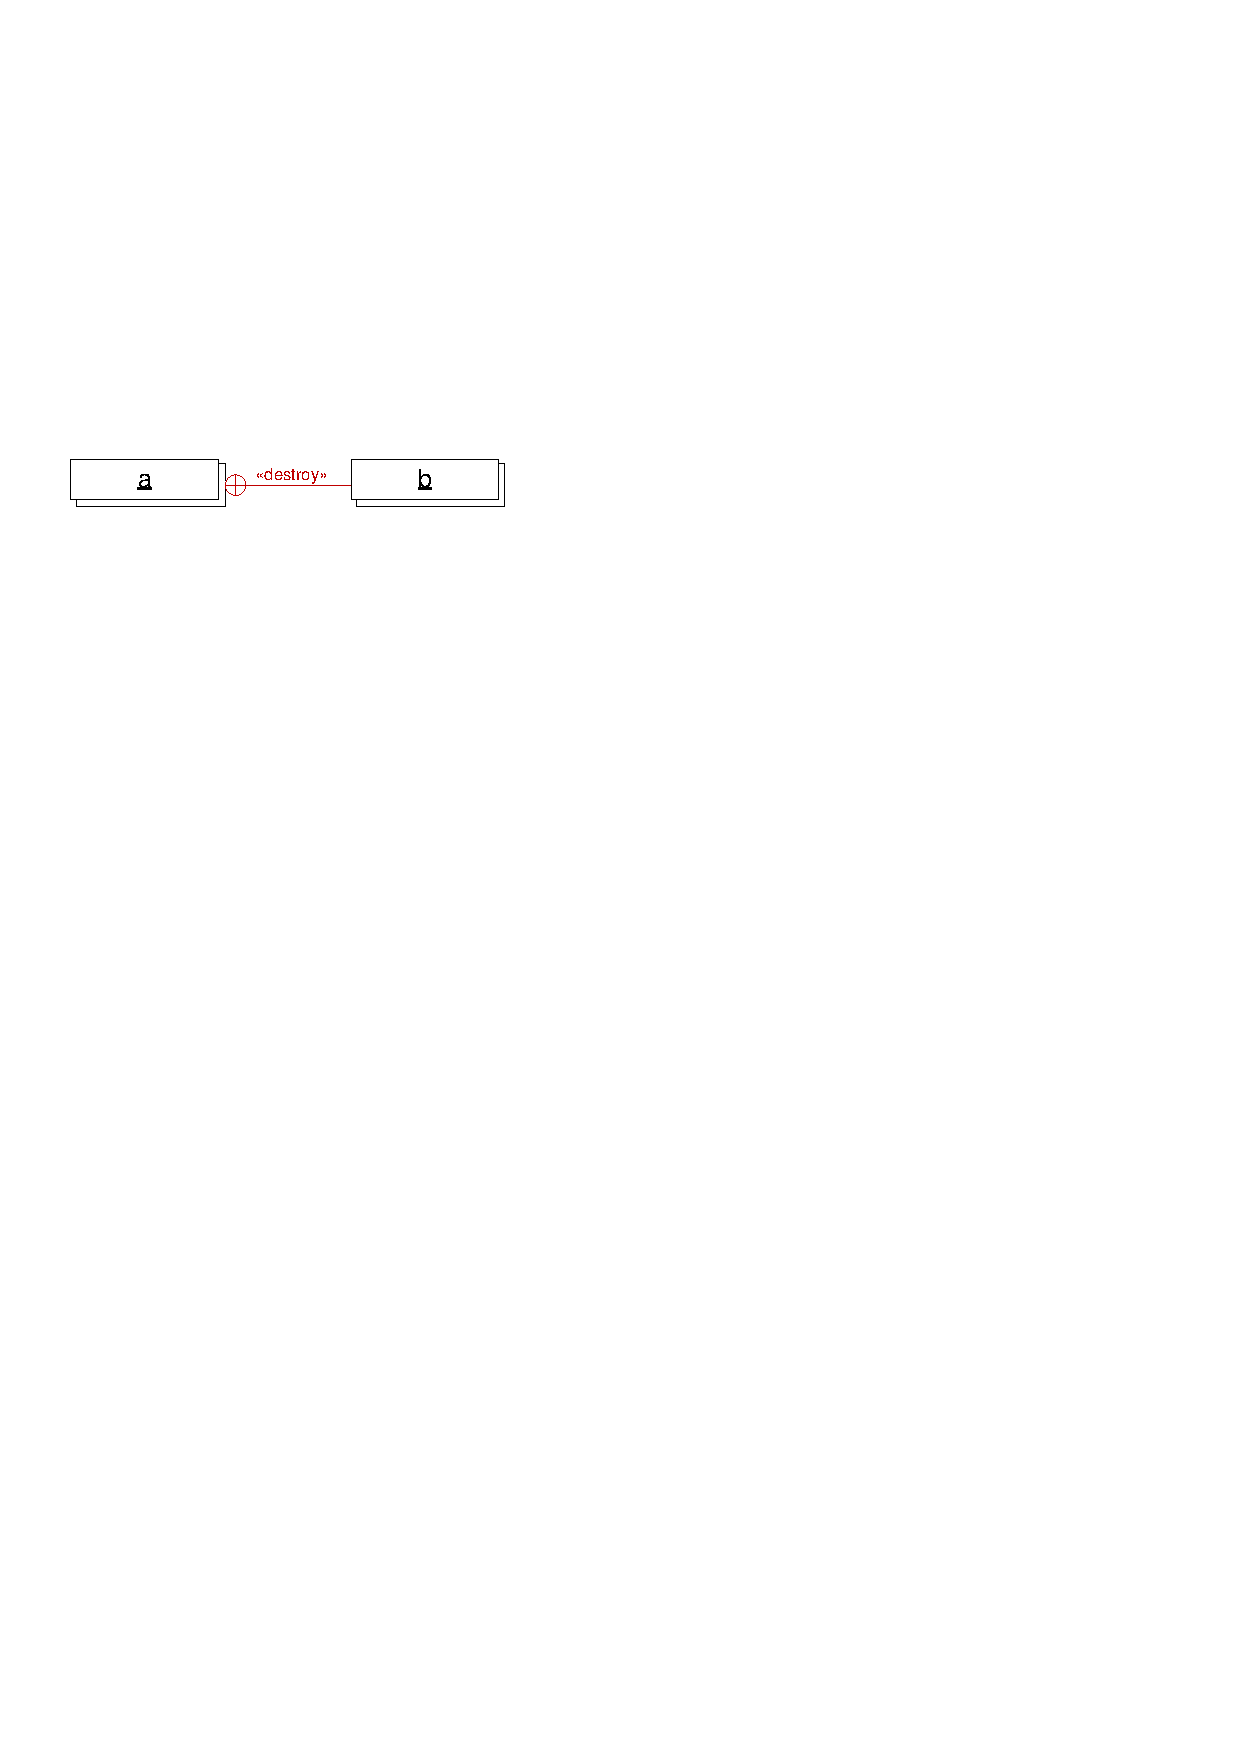
\includegraphics[scale=0.8]{figures/InclusionLinksSetsDestroy}
    } & \\
    \hline
    Ordered Set & any & DESTROY & Remove all elements in \fe{b} from \fe{a}, preserve the order of remaining elements in \fe{a}.\\[0.5em]
    List & Ordered Set & DESTROY & Remove \emph{all} occurrences of elements contained in \fe{b} from \fe{a}, preserve the order of remaining elements in \fe{a}.\\[0.5em]
    List & List & DESTROY & Starting at the beginning of the list \fe{a}, for each element in \fe{b} remove as many occurrences of the element in \fe{a} as it is available in \fe{b}, preserve the order of remaining elements in \fe{a}.\\
    \hline
    \end{tabular}
%  \end{longtable}
\end{table}


%\ext %--- Comment this line to include link constraints into the
{
\subsection{Link Constraints}
\label{sec:StoryPatterns:linkConstraints}

\tododt{The link constraints section is existing twice.}

Link constraints specify constraints on the absolute position of an element in an ordered reference (\emph{link position constraints}, Section~\ref{sec:StoryPatterns:linkConstraints:posConstraint}) or on the position of an element relative to another element (\emph{link order constraints}, Section~\ref{sec:StoryPatterns:linkConstraints:orderConstraint}). These constraints are only applicable to link variables that are typed by ordered multi-valued references. All other kinds of links cannot be adorned with link constraints.

%\begin{itemize}
%  \item FIRST = matches the first element in the list, requires one link variable
%  \item LAST = matches the last element in the list, requires one link variable
%%  \item INDEX = matches the element at the specified index, requires one link variable
%%  \todoch{Our lowest index value is 0, not 1.}
%  \item DIRECT\_SUCCESSOR = requires two link variables, target of the second one must be located directly after the target of the first one in the list
%  \item SUCCESSOR = requires two link variables, target of the second one must be located somewhere after the target of the first one in the list
%\end{itemize}


\subsubsection{Link Position Constraints}
\label{sec:StoryPatterns:linkConstraints:posConstraint}

A link position constraint applies to a link variable that is typed by a multi-valued ordered reference. It specifies that the target object of the constrained link has to be the \emph{first} or the \emph{last} element in that reference. Other link position constraints are not supported. 

The \emph{index} link constraint, which was available in earlier versions of story diagrams~\cite{WW01_ag}, is no longer supported. 
It was used to match an element which is located at a specific position in a multi-valued reference. 
However, that causes that upon creation of multiple elements it is not precisely defined where they are inserted into the list. 
In addition, the index may cause \emph{OutOfBounds} exceptions if the modeler specifies an invalid index.

Figure~\ref{fig:linkPositionConstraintFirst} shows an example of a link position constraint for matching the first element in a reference. The story pattern matches a \fe{FormalParameter} of the object which is bound to the object variable \fe{method}. The link position constraint \fe{\{first\}} specifies that the first \fe{FormalParameter} needs to be matched.

\begin{figure}[htbp]
\center
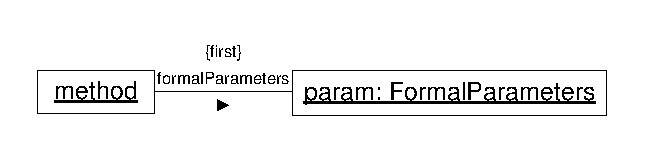
\includegraphics[width=0.75\columnwidth]{figures/LinkPositionConstraintFirst}
\caption{A \fe{\{first\}} link position constraint}
\label{fig:linkPositionConstraintFirst}
\end{figure}

Figure~\ref{fig:linkPositionConstraintLast} shows a similar story pattern, which matches the last \fe{FormalParameter} instead of the first one. This is specified by the link position constraint \fe{\{last\}}.

\begin{figure}[htbp]
\center
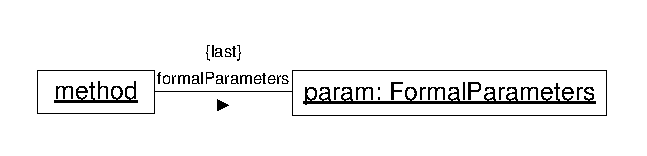
\includegraphics[width=0.75\columnwidth]{figures/LinkPositionConstraintLast}
\caption{A \fe{\{last\}} link position constraint}
\label{fig:linkPositionConstraintLast}
\end{figure}

If multiple link variables originate from the same object variable that refer to the same reference, only one of them may have a \fe{\{first\}} (or \fe{\{last\}}) link position constraint.

Link position constraints can be used with all feasible combinations of binding operators and binding semantics according to Table~\ref{tab:bindingCombinations_links}. For now, we discussed the semantics for using link position constraints for link variables with MANDATORY binding semantics and CHECK\_ONLY binding operator. If we use binding operator \create, the object is inserted at the specified position.
If the target element already exists in the reference but at a different position, the semantics of the create depends on the kind of the reference. 
If the reference requires objects to be unique in the reference, the target element is moved to the position specified by the create link variable. 
Otherwise, the element is added a second time at the specified position.
If we use binding operator \destroy, the object is bound as described before and then deleted.

Figure~\ref{fig:linkPositionConstraintCreate} shows an example for using a link position constraint at a link variable with binding operator \create. The link position constraint causes the created \fe{FormalParameter} to be inserted at the last position of the \fe{formalParameters} of \fe{method}.

\begin{figure}[htbp]
\center
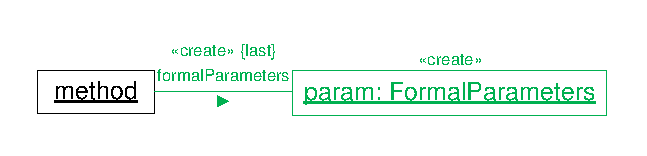
\includegraphics[width=0.75\columnwidth]{figures/LinkPositionConstraintCreate}
\caption{Link Position constraint at a created link.}
\label{fig:linkPositionConstraintCreate}
\end{figure}

If an OPTIONAL binding semantics is used, the matching will also be successful if no object at the specified position can be matched. Since we only restrict the position to the first or last position, this case will only apply if the link contains no objects at all. If the link variable additionally has binding operator \destroy, the object bound to the target object variable will be deleted. If the link variable additionally has binding operator \create, we have an optionally created link. If the object does not yet exist at the specified position, it is inserted following the rules for created links as described before. 

A combination with NEGATIVE binding semantics is also possible. If a link variable is negative and has a \fe{\{first\}} (or \fe{\{last\}}) link position constraint, then the object bound to the target object variable must not be the first (or last) object in the corresponding reference. That means, we negate the link position constraint rather than the whole link variable which causes a slight change of the NEGATIVE binding semantics of link variables.

%\todoch{How is the semantics of link position constraints on negative links as shown in Figure~\ref{fig:linkPositionConstraintNegative}? Two alternatives: 1) The target object is not the first (or last) element in the reference. That means we negate the link position constraint and not the whole link variable. 2) There exists no link pointing to the first (or last) element. That means we negate the whole link which in turn means that there is no element in the reference and the link position constraint has no effect. I prefer 1) even though it slightly changes the semantics of the negative binding semantics (because it is applied to the link constraint rather than the link itself).}

Figure~\ref{fig:linkPositionConstraintNegative} shows an example for a negative link with a link position constraint. The \fe{FormalParameter} which is bound to \fe{param} must not be the first \fe{formalParameter} of the method which is bound to \fe{method}.


\begin{figure}[htbp]
\center
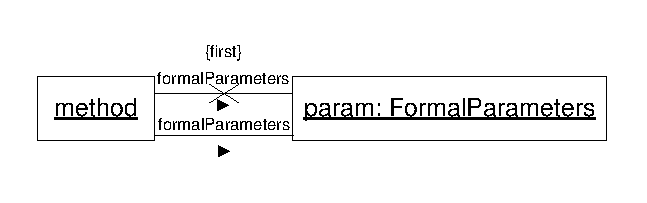
\includegraphics[width=0.75\columnwidth]{figures/LinkPositionConstraintNegated}
\caption{A negative link with a \fe{\{first\}} link position constraint}
\label{fig:linkPositionConstraintNegative}
\end{figure}



\subsubsection{Link Order Constraints}
\label{sec:StoryPatterns:linkConstraints:orderConstraint}

Link order constraints specify a relative order between two objects in a multi-valued ordered reference. A link order constraint therefore connects two link variables which we denote as the source link variable and target link variable of the link order constraint. Then, the object matched via the target link variable must either be the \emph{direct successor} or an  \emph{arbitrary successor} of the object matched via the source link variable.

Figure~\ref{fig:linkOrderConstraintDirectSuccessor} shows an example of a link order constraint requiring to match two subsequent \fe{FormalParameters} of \fe{method}. Therefore, the two link variables from \fe{method} to \fe{param1} and \fe{param2} are connected by a link order constraint \fe{\{next\}}. Then, the object matched to \fe{param2} must be a direct successor of the object matched to \fe{param1}.

\begin{figure}[htbp]
\center
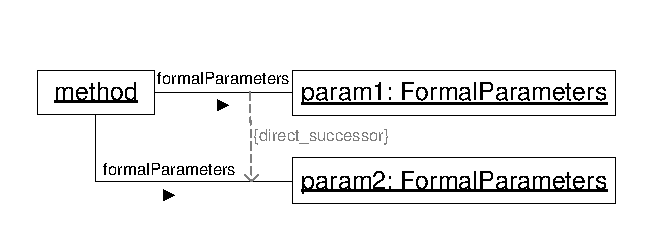
\includegraphics[width=0.75\columnwidth]{figures/LinkOrderConstraintDirectSuccessor}
\caption{A link order constraint specifying a \fe{\{direct\_successor\}}.}
\label{fig:linkOrderConstraintDirectSuccessor}
\end{figure}

Figure~\ref{fig:linkOrderConstraintSuccessor} shows an example of a link order constraint requiring to match two \fe{FormalParameters} of \fe{method} where one succeeds the other. Therefore, the two link variables from \fe{method} to \fe{param1} and \fe{param2} are connected by a link order constraint \fe{\{successor\}}. Then, the object matched to \fe{param2} must be an arbitrary successor of the object matched to \fe{param1}. The matching of the successor is non-deterministic. Thus, a matching retrieved for the story pattern in Figure~\ref{fig:linkOrderConstraintDirectSuccessor} is a valid matching for the story pattern in Figure~\ref{fig:linkOrderConstraintSuccessor} as well. A matching retrieved for the story pattern in Figure~\ref{fig:linkOrderConstraintSuccessor}, however, will not be a valid matching for the story pattern in Figure~\ref{fig:linkOrderConstraintDirectSuccessor} in the general case.

\begin{figure}[htbp]
\center
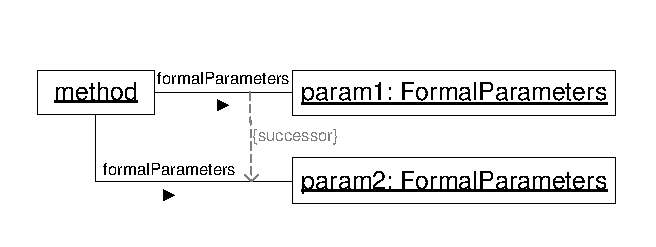
\includegraphics[width=0.75\columnwidth]{figures/LinkOrderConstraintSuccessor}
\caption{A link order constraint specifying a \fe{\{successor\}}.}
\label{fig:linkOrderConstraintSuccessor}
\end{figure}

Link order constraints can be applied to links that have a binding operator \create or \destroy. In case of \destroy, the matching is carried out as described before. In case of \create, links corresponding to the link variables are created in the instance model. The target objects are then inserted into the reference at the specified positions. If the source link variable (or target link variable) of the link order constraint has a \create binding operator, then the object is inserted directly before (or after) the object bound via the target (or source) link variable. We also apply this semantics if the link order constraint requires the objects only to be indirect successors to avoid non-determinism.

\begin{figure}[htbp]
\center
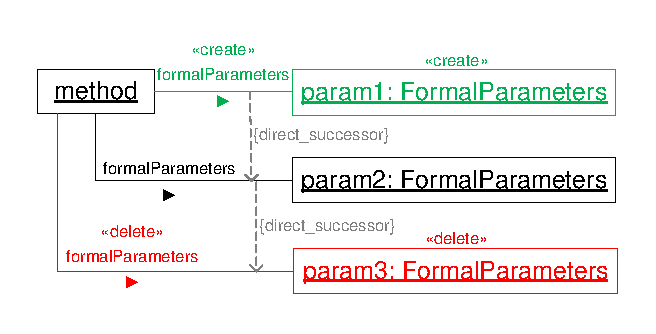
\includegraphics[width=0.75\columnwidth]{figures/LinkOrderConstraintDirectSuccessorCreateDelete}
\caption{Using link order constraints with binding operators \create and \destroy.}
\label{fig:linkOrderConstraintDirectSuccessorCreateDelete}
\end{figure}

Figure~\ref{fig:linkOrderConstraintDirectSuccessorCreateDelete} shows an example for using link order constraints with the binding operators \create and \destroy. The story pattern matches two successive \fe{FormalParameters} of \fe{method} and binds them to the object variables \fe{param2} and \fe{param3}. If the matching was successful, the parameter bound to \fe{param3} is deleted and removed from the reference. Then, a new \fe{FormalParameter} is created and inserted directly before \fe{param2}.

If a link variable with binding operator \create is the target link variable (or source link variable) of several \emph{indirect successor} link order constraints, then the target object of the link variable is inserted directly behind (or before) the object with the highest index. If  multiple link constraints are applied to the same link variable with binding operator \create, enforcing the right-hand side of the story pattern may fail if the link constraints are unsatisfiable for the reference.

If the reference already contains the target object of a create link variable, but at a position which does not satisfy the link order constraint, then there are two possibilities.  If the reference requires objects to be unique in the reference, the target element is moved to a position specified by the link order constraints. Otherwise, the element is added a second time at a position specified by the link order constraints. 

If both, the source link variable and the target link variable of the link order constraint, carry a binding operator, both need to carry the same binding operator. If one link variable has a binding operator \create and the other one has \destroy, then the reference for inserting the new object has been deleted before the object can be inserted. Since the semantics in undefined in that case, we forbid this case.

Link order constraints can be used in combination with an optional binding semantics of the source or target link variable. In case the link variable carries no binding operator or binding operator \destroy, the matching process is performed as described before. If no matching for the optional link variables satisfying the link order constraints can be found, the matching does not fail. If the a link variable carries an optional create, a matching which satisfies the link order constraints is searched. If no matching can be obtained, the rules for inserting an object into a reference as described above for non-optional link variables are applied.

Link order constraints may also be used in combination with a negative binding semantics of the source or target link variable. If a negative link variable is the target link variable of a \emph{direct successor} (or \emph{indirect successor}) link order constraint, then the target object must not be located directly after (of indirectly after) the object bound to the source link variable. If a negative link variable is the source link variable of a \emph{direct successor} (or \emph{indirect successor}) link order constraint, then the target object must not be located directly before (of indirectly before) the object bound to the target link variable. That means, we negate the link order constraint rather than the whole link variable if the link variable is the source or target link variable of a link order constraint. That causes a slight change in the definition of the negative binding semantics for link variables.

\begin{figure}[htbp]
\center
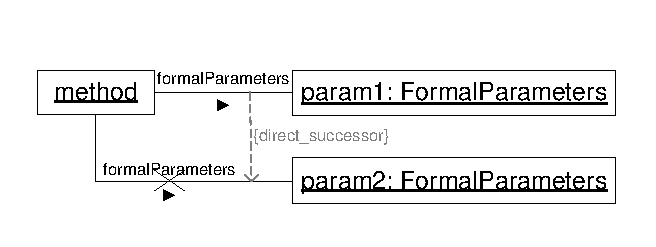
\includegraphics[width=0.75\columnwidth]{figures/LinkOrderConstraintDirectSuccessorNegative}
\caption{A link order constraint with a negative link.}
\label{fig:linkOrderConstraintDirectSuccessorNegative}
\end{figure}

Figure~\ref{fig:linkOrderConstraintDirectSuccessorNegative} shows an example of a negative link variable which is the target link variable of a \emph{direct successor} link order constraint. In the example, two \fe{FormalParameters} of \fe{method} are to be matched. The object bound to \fe{param1} may be an arbitrary \fe{FormalParameter}. The object variable \fe{param2} may be matched to any \fe{FormalParameter} of \fe{method} except for the \fe{FormalParameter} that is directly located behind the object bound to \fe{param1}.

It is possible to use multiple link order constraints on a negative link. Then, all of the specified conditions need to hold. However, for each link order constraint either the source link variable or the target link variable may be negative, but not both.

\begin{figure}[htbp]
\center
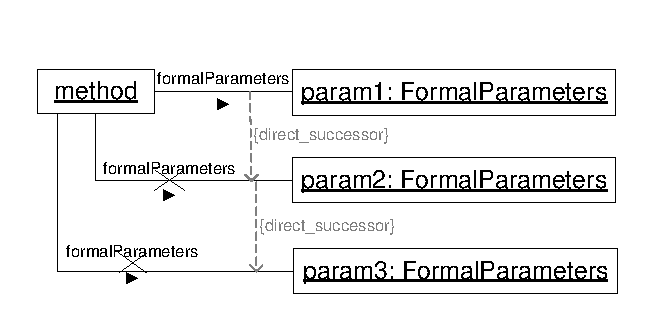
\includegraphics[width=0.75\columnwidth]{figures/LinkOrderConstraintDirectSuccessorNegative2}
\caption{Applying Multiple Link Order Constraints on a Negative Link Variable}
\label{fig:linkOrderConstraintDirectSuccessorNegative2}
\end{figure}

Figure~\ref{fig:linkOrderConstraintDirectSuccessorNegative2} shows an example of applying multiple link order constraint to a negative link variable. The story pattern matches three \fe{FormalParameters} of \fe{method}. The matching must fulfill the following conditions which are implied by the negative link variable from \fe{method} to \fe{param2} and the two link order constraints: \fe{param2} must not be an indirect successor of \fe{param1} and \fe{param3} must not be the direct successor of \fe{param2}. If only one of the two conditions is not fulfilled, then the story pattern does not match.

\begin{figure}[htbp]
\center
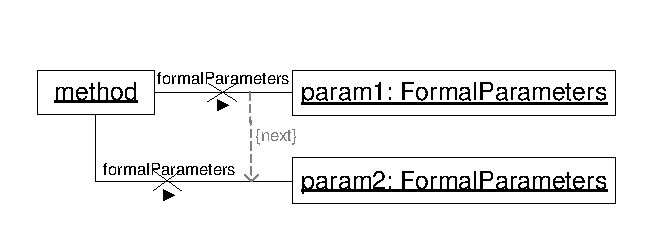
\includegraphics[width=0.75\columnwidth]{figures/LinkOrderConstraintDirectSuccessorNegative3}
\caption{Invalid Combination of Link Order Constraints and Negative Link Variables.}
\label{fig:linkOrderConstraintDirectSuccessorNegative3}
\end{figure}

Figure~\ref{fig:linkOrderConstraintDirectSuccessorNegative3} shows an example of an invalid combination of negative link variables and link order constraints because both, the source and the target link variable of the link order constraint, are negative. 

Link order constraints may not form circles or unsatisfiable story patterns. An example of an unsatisfiable story pattern is given by Figure~\ref{fig:linkConstraintUnsatisfiablePattern}. In this story pattern, the object bound to \fe{param2} must be the first \fe{FormalParameter} of \fe{method}. At the same time, the link order constraint requires the object bound to \fe{param2} to be the direct successor of the object bound to \fe{param1}. Since this is not possible, the pattern is unsatisfiable and will never match.


\begin{figure}[htbp]
\center
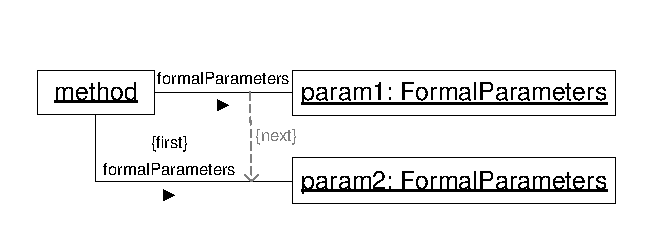
\includegraphics[width=0.75\columnwidth]{figures/LinkConstraintUnsatisfiablePattern}
\caption{Link Constraints causing a Story Pattern to be unsatisfiable.}
\label{fig:linkConstraintUnsatisfiablePattern}
\end{figure}

By supporting sequences of link order constraints (cf. Figure~\ref{fig:linkOrderConstraintDirectSuccessorCreateDelete}) and combinations of link position and link order constraints, we extend story patterns and their semantics as proposed by Tichy et. al.~\cite{TMG06}. The general semantical issue that the insertion into an ordered reference is non-deterministic remains, but may be explicitly solved using the link constraints introduced in this section. 

\begin{figure}[htb]
  \centering
  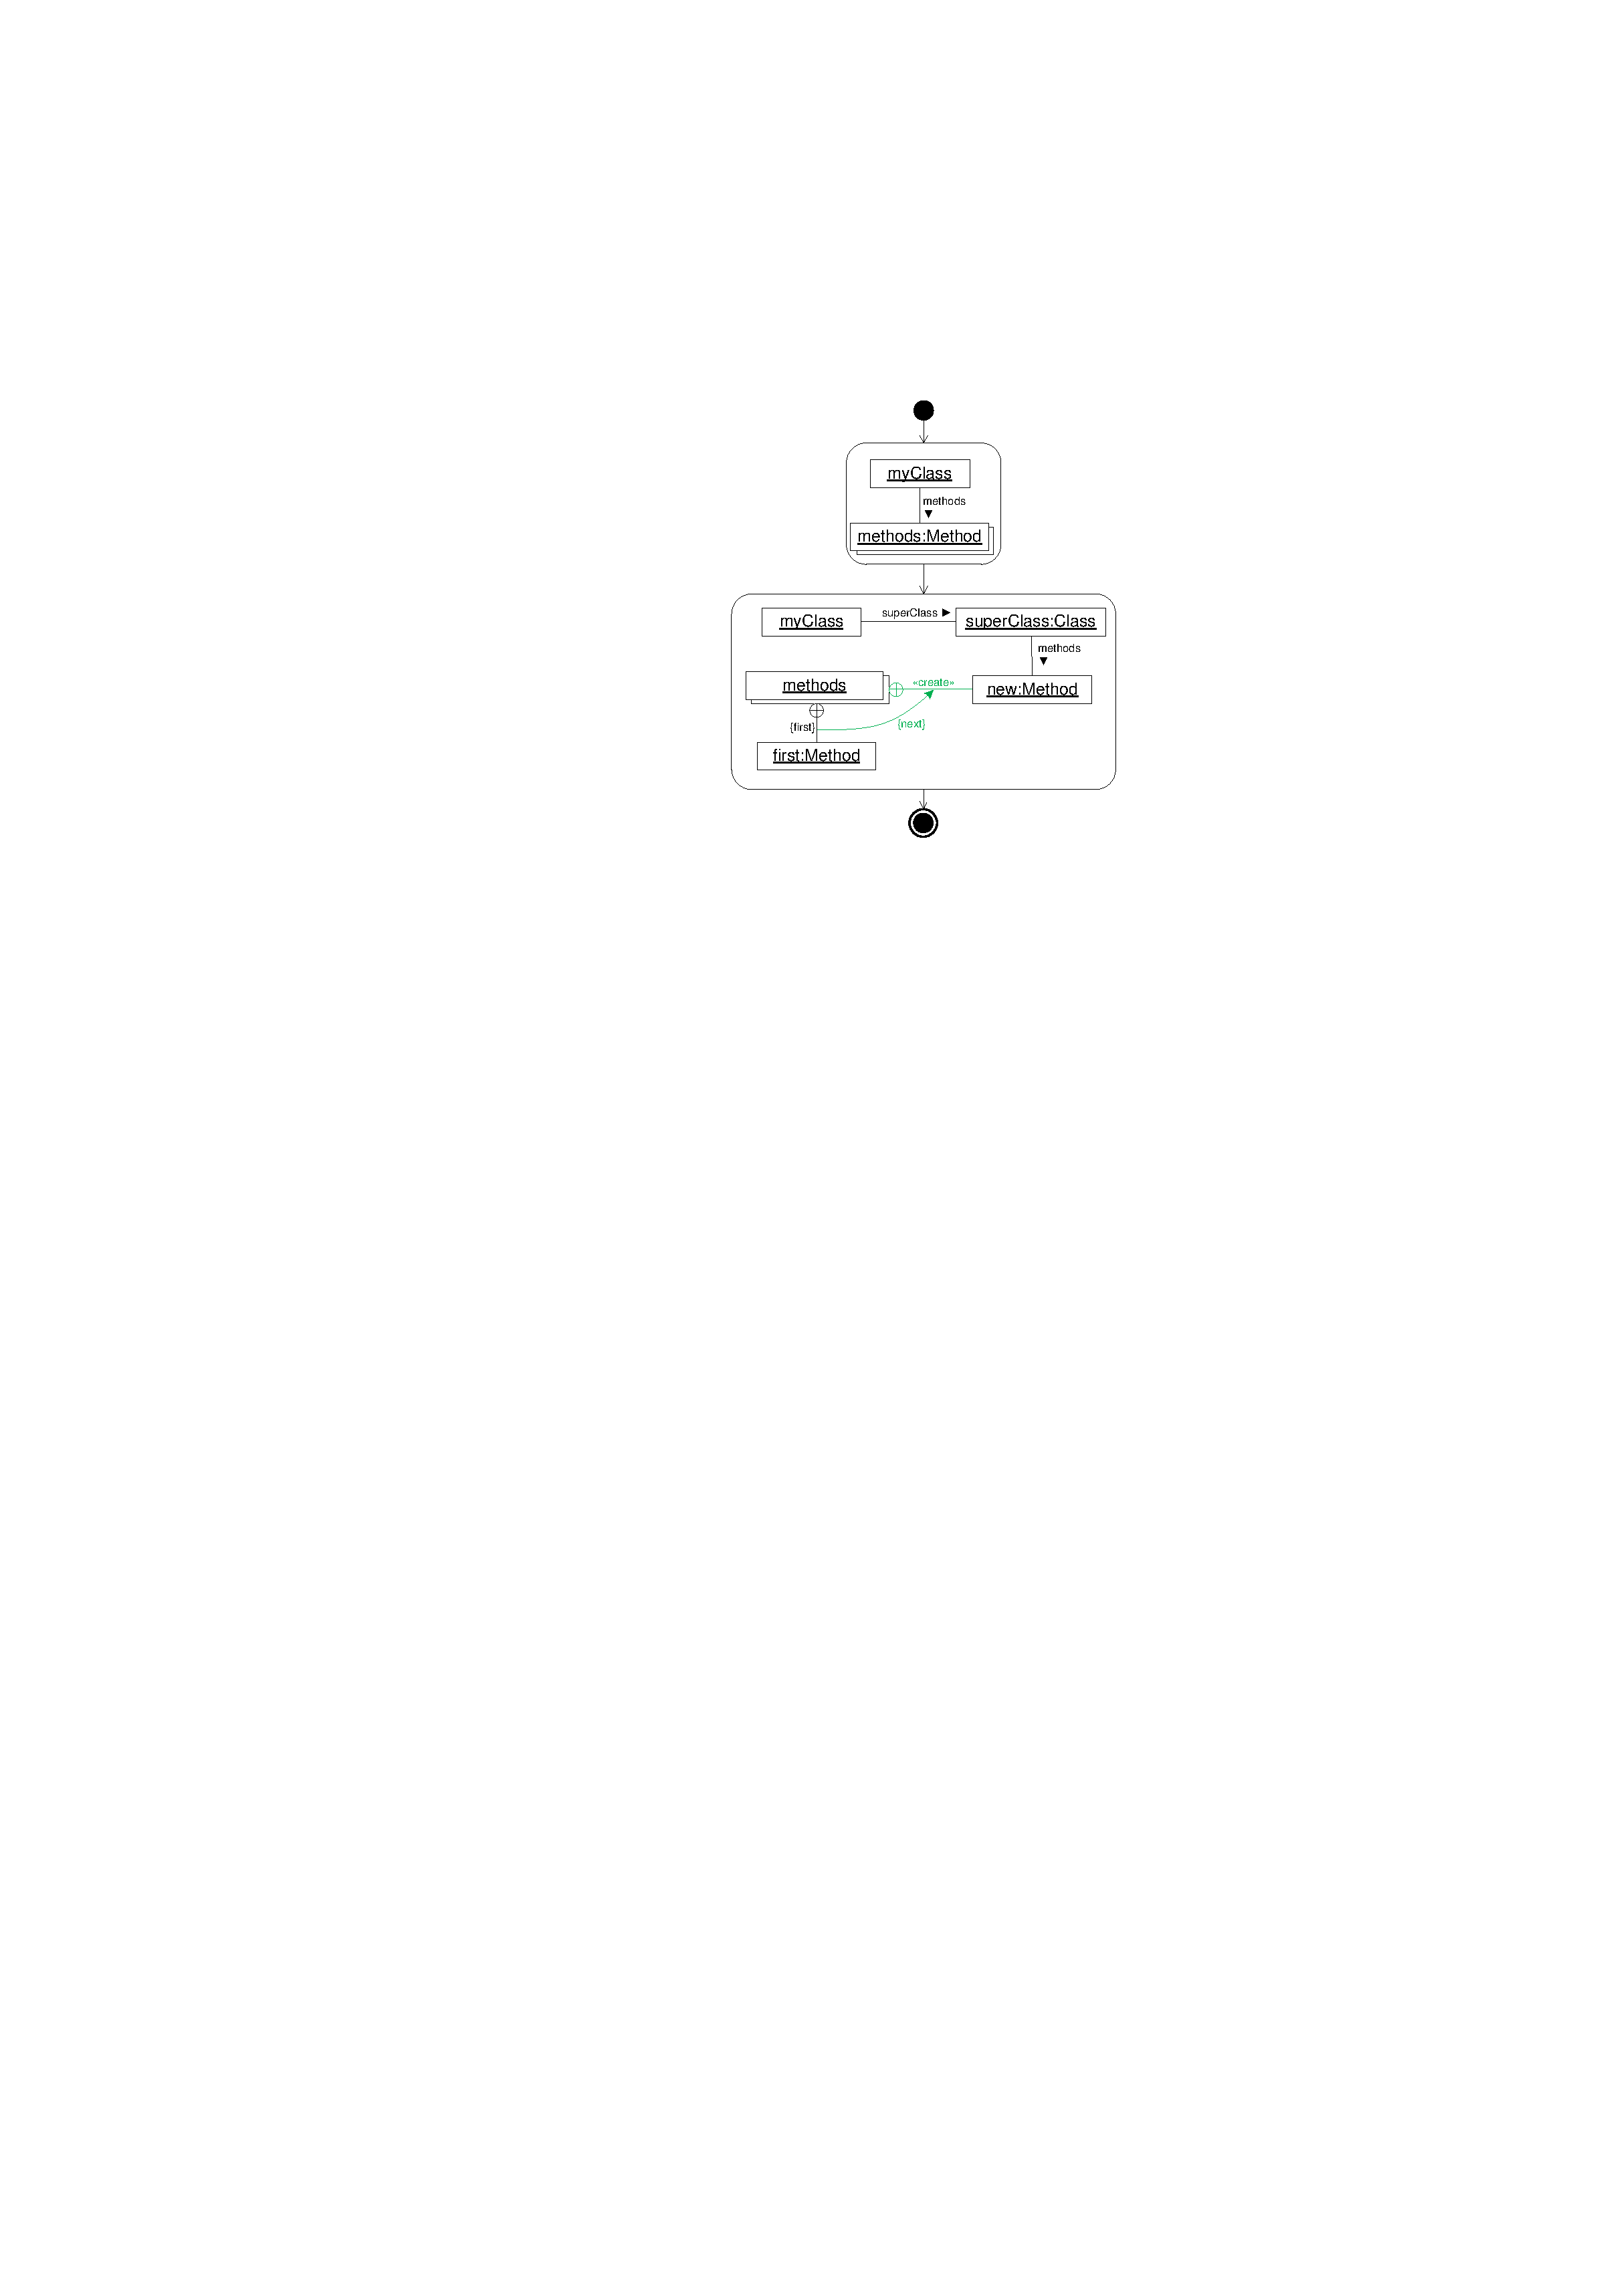
\includegraphics[scale=.8]{figures/LinkConstraints1}
  \caption{Inclusion Links With Link Constraints}
  \label{fig:collectionsLinkConstraints}
\end{figure}

Similar to the link constraints described in Section~\ref{sec:StoryPatterns:linkConstraints}, link constraints can also be used with inclusion links.
An exemplary use is illustrated in the story diagram in Figure~\ref{fig:collectionsLinkConstraints}.
We will explain story diagrams in more detail in Section~\ref{sec:StoryDiagrams}.
Here, the story diagram describes the sequential execution of two story patterns.

In the first story pattern (the upper one), a set of \fe{Method} objects is collected from a given class \fe{myClass} and stored in the collection \fe{methods}.
In the next story pattern, a superclass of \fe{myClass}, a method in this superclass and the first method in the collection \fe{methods} are matched.
In case of a successful matching the newly matched method \fe{new} is added to the collection \fe{methods}.
The link constraint \fe{\text\{next\text\}} determines to add this method to the ordered collection in such a way
that the method \fe{new} directly follows the method \fe{first} in the collection \fe{methods}.



} %--- End of link constraint subsection

\subsection{Maybe Links}
\label{sec:StoryPatterns:specialLinks:maybeLink}

Story patterns are matched by using isomorphic matchings. 
That means that two object variables in a story pattern may not be matched to the same object of the instance model. 
A matching which matches two object variables to the same object is, thus, considered to be invalid. 
In some situations, however, it should be explicitly allowed to match the same object to two different object variables inside the same story pattern. 
Then, the isomorphic matching must be disabled for the two corresponding object variables. 
This is achieved by connecting the object variables with a maybe link. 
Then, a matching \emph{may} assign the same object to the object variables connected by the maybe link, but it also may assign different objects to the variables.
For all other object variables, the isomorphism condition is enforced.


%\tododt{Please clarify the semantics of a \emph{maybe} link.
%It allows two object variables to be matched to the same object.
%For all aother variables an isomorphic matching is performed.
%I would also emphasize \emph{maybe}.}

\begin{figure}[htb]
  \centering
  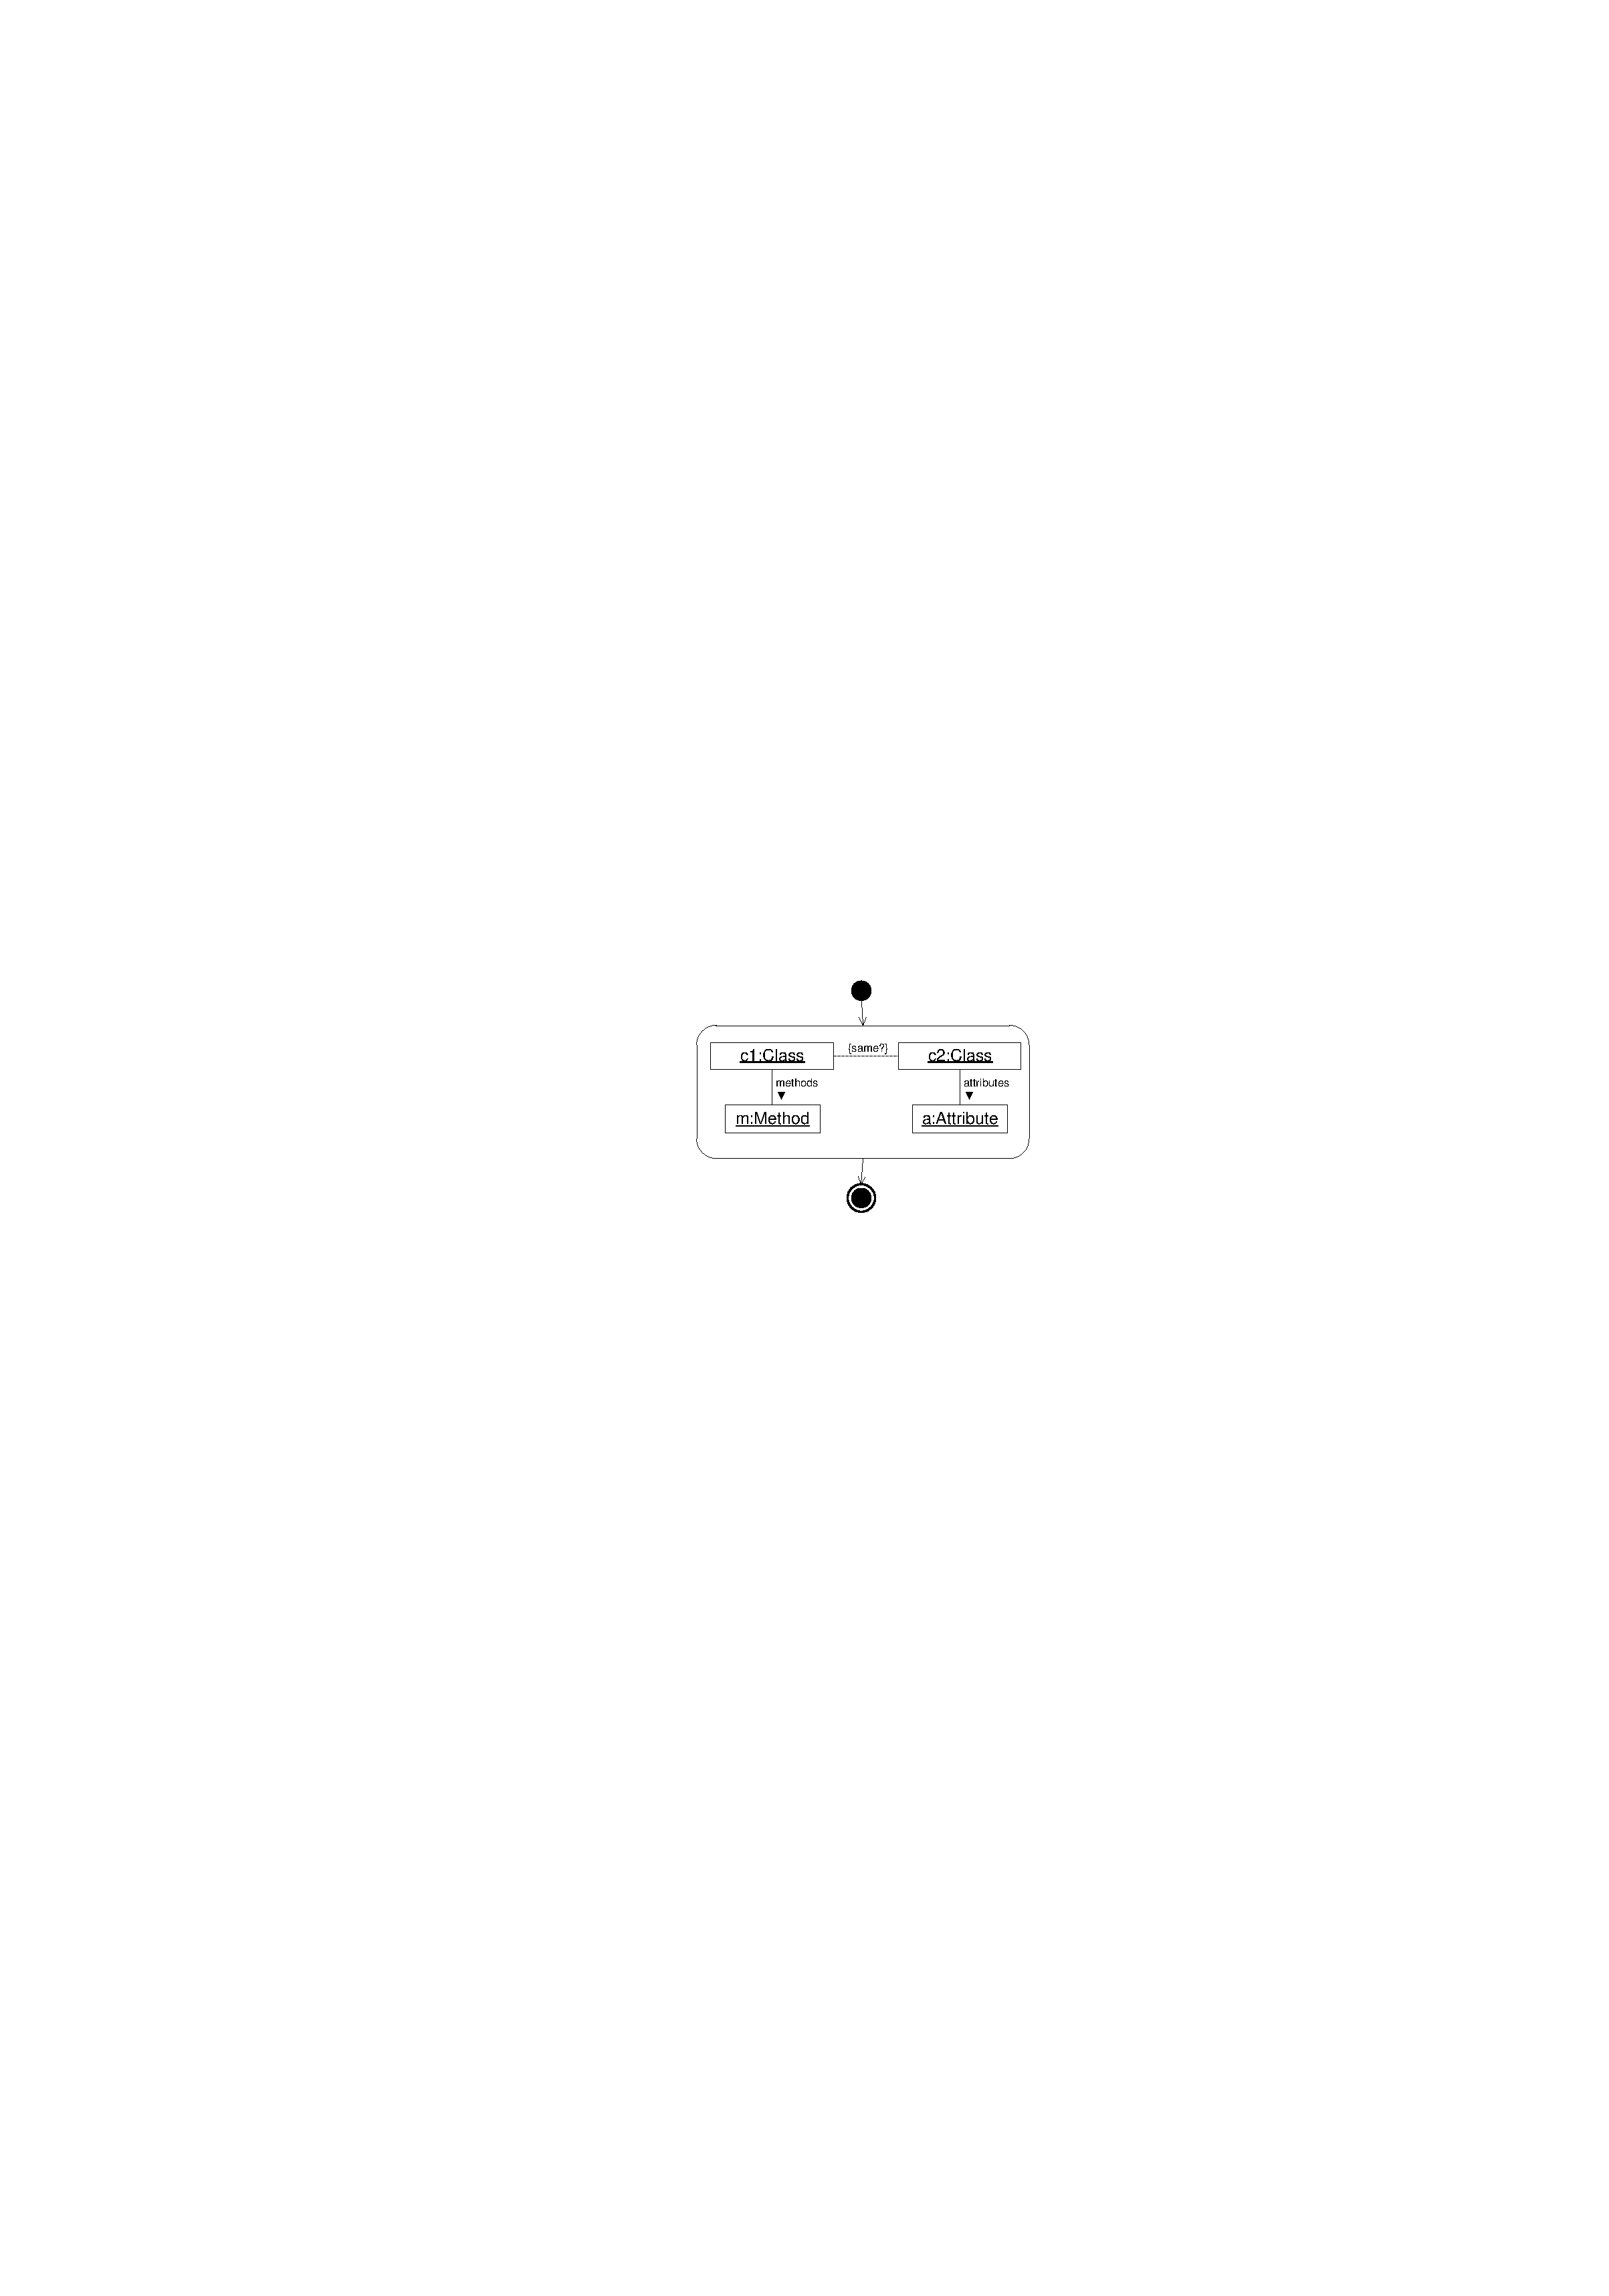
\includegraphics[scale=.8]{figures/MaybeLink}
  \caption{Maybe Link allowing two Object Variables to be matched to the same Object}
  \label{fig:maybeLink}
\end{figure}

Figure \ref{fig:maybeLink} shows the concrete syntax of maybe links. The object variables \fe{c1} and \fe{c2} are connected with a maybe link which is visualized by a dotted line labeled with \fe{\{same\}}.
The matching of the story patterns is successful if either two classes - one containing a method and one containing an attribute - can be matched in the instance graph \emph{or} if only one class containing a method \emph{and} an attribute can be matched.

If two object variables are connected by a maybe link, they both must be mandatory or optional. In addition, a maybe link requires the object variables to be matched or destroyed, but not created.  


%\ext  %--- Comment this line to include pattern constraints into the document
{
\subsection{Pattern Constraints}
\label{sec:PatternConstraints}

A pattern constraint defines an additional condition for a match that is evaluated and the end of the matching step, i.e., it is evaluated after all object and link variables have been matched. Since it is a condition, it needs to evaluate to true or false. If the pattern constraint is evaluated to true, then the match for the story pattern is valid. If the pattern constraint is evaluated to false, then the match is rejected.

A pattern constraint may use all object variables that are used in the same story pattern. Object variables are referred by their name. The pattern constraint may traverse the references of the objects bound to a particular object variable and access the attributes of the corresponding object. In the current version of story diagrams, we only support to use OCL for specifying pattern constraints. Then, the OCL constraint uses the name of the object variables to refer to objects and may use all features of OCL to access references and attributes of the corresponding objects.

\begin{figure}[htbp]
\center
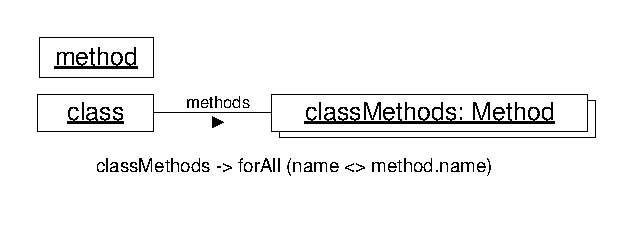
\includegraphics[width=0.6\columnwidth]{figures/PatternConstraint}
\caption{Example of a Pattern Constraint}
\label{fig:patternConstraint}
\end{figure}

\tododt{Should the constraint in Figure~\ref{fig:patternConstraint} not be classMethods->forAll(name <> method.name)? Otherwise the constraint does not check the matched methods in \fe{classMethods}.}

Figure~\ref{fig:patternConstraint} gives an example for the concrete syntax of a pattern constraint. The story pattern has two bound object variables \fe{class} and \fe{method} of types \fe{GASTClass} and \fe{Method}, respectively. The pattern constraint is visualized as a label containing the OCL constraint. In the example, the OCL constraints specifies that all methods of \fe{class} need to have a name which is different from the name of \fe{method}. In addition, the story pattern matches all methods of \fe{class} in the object set \fe{classMethods}. The matching of the story pattern is successful only if the pattern constraint is fulfilled.

} %--- End of pattern constraints section




\ext %--- Comment this line to include paths into the document
{ 
\subsection{Paths [MCP]}
\label{sec:StoryPatterns:paths}
} %--- End of paths subsection


\ext  %--- Comment this line to include pattern fragments into the document
{
\subsection{Pattern Fragments [MCP]}

patterns contained in other patterns, negative, semantics? review enhanced story patterns from Diss Florian Klein

\todomcp{Should contained pattern be marked as forEach? Idea for semantics: first the part of the pattern outside the forEach pattern is matched, then the forEach subpattern is applied to any match that may be located, the variables bound in a forEach subpattern may not be used in subsequent activities}

\todoch{The transformations diagrams that Matthias Meyer developed in his Diss contain so-called iterated parts that are essentially the same as a for-each fragment. We should check his semantics.}

\tododt{This is somewhat confusing.
As I understand them, subpatterns are ordinary story patterns within another story pattern.
They are surrounded by a fragment box and can be labeled with a name (see Figure~\ref{fig:labeledSubPattern}).
Special types of such subpatterns are negative application condition fragments (NACs), set fragments, and optional fragments.
As far as I know, we did not plan to add $\forall$ and $\exists$ fragments, did we?
These are only used in SDDs and TSSDs which are constraint languages.
}

\begin{figure}[htbp]
  \centering
  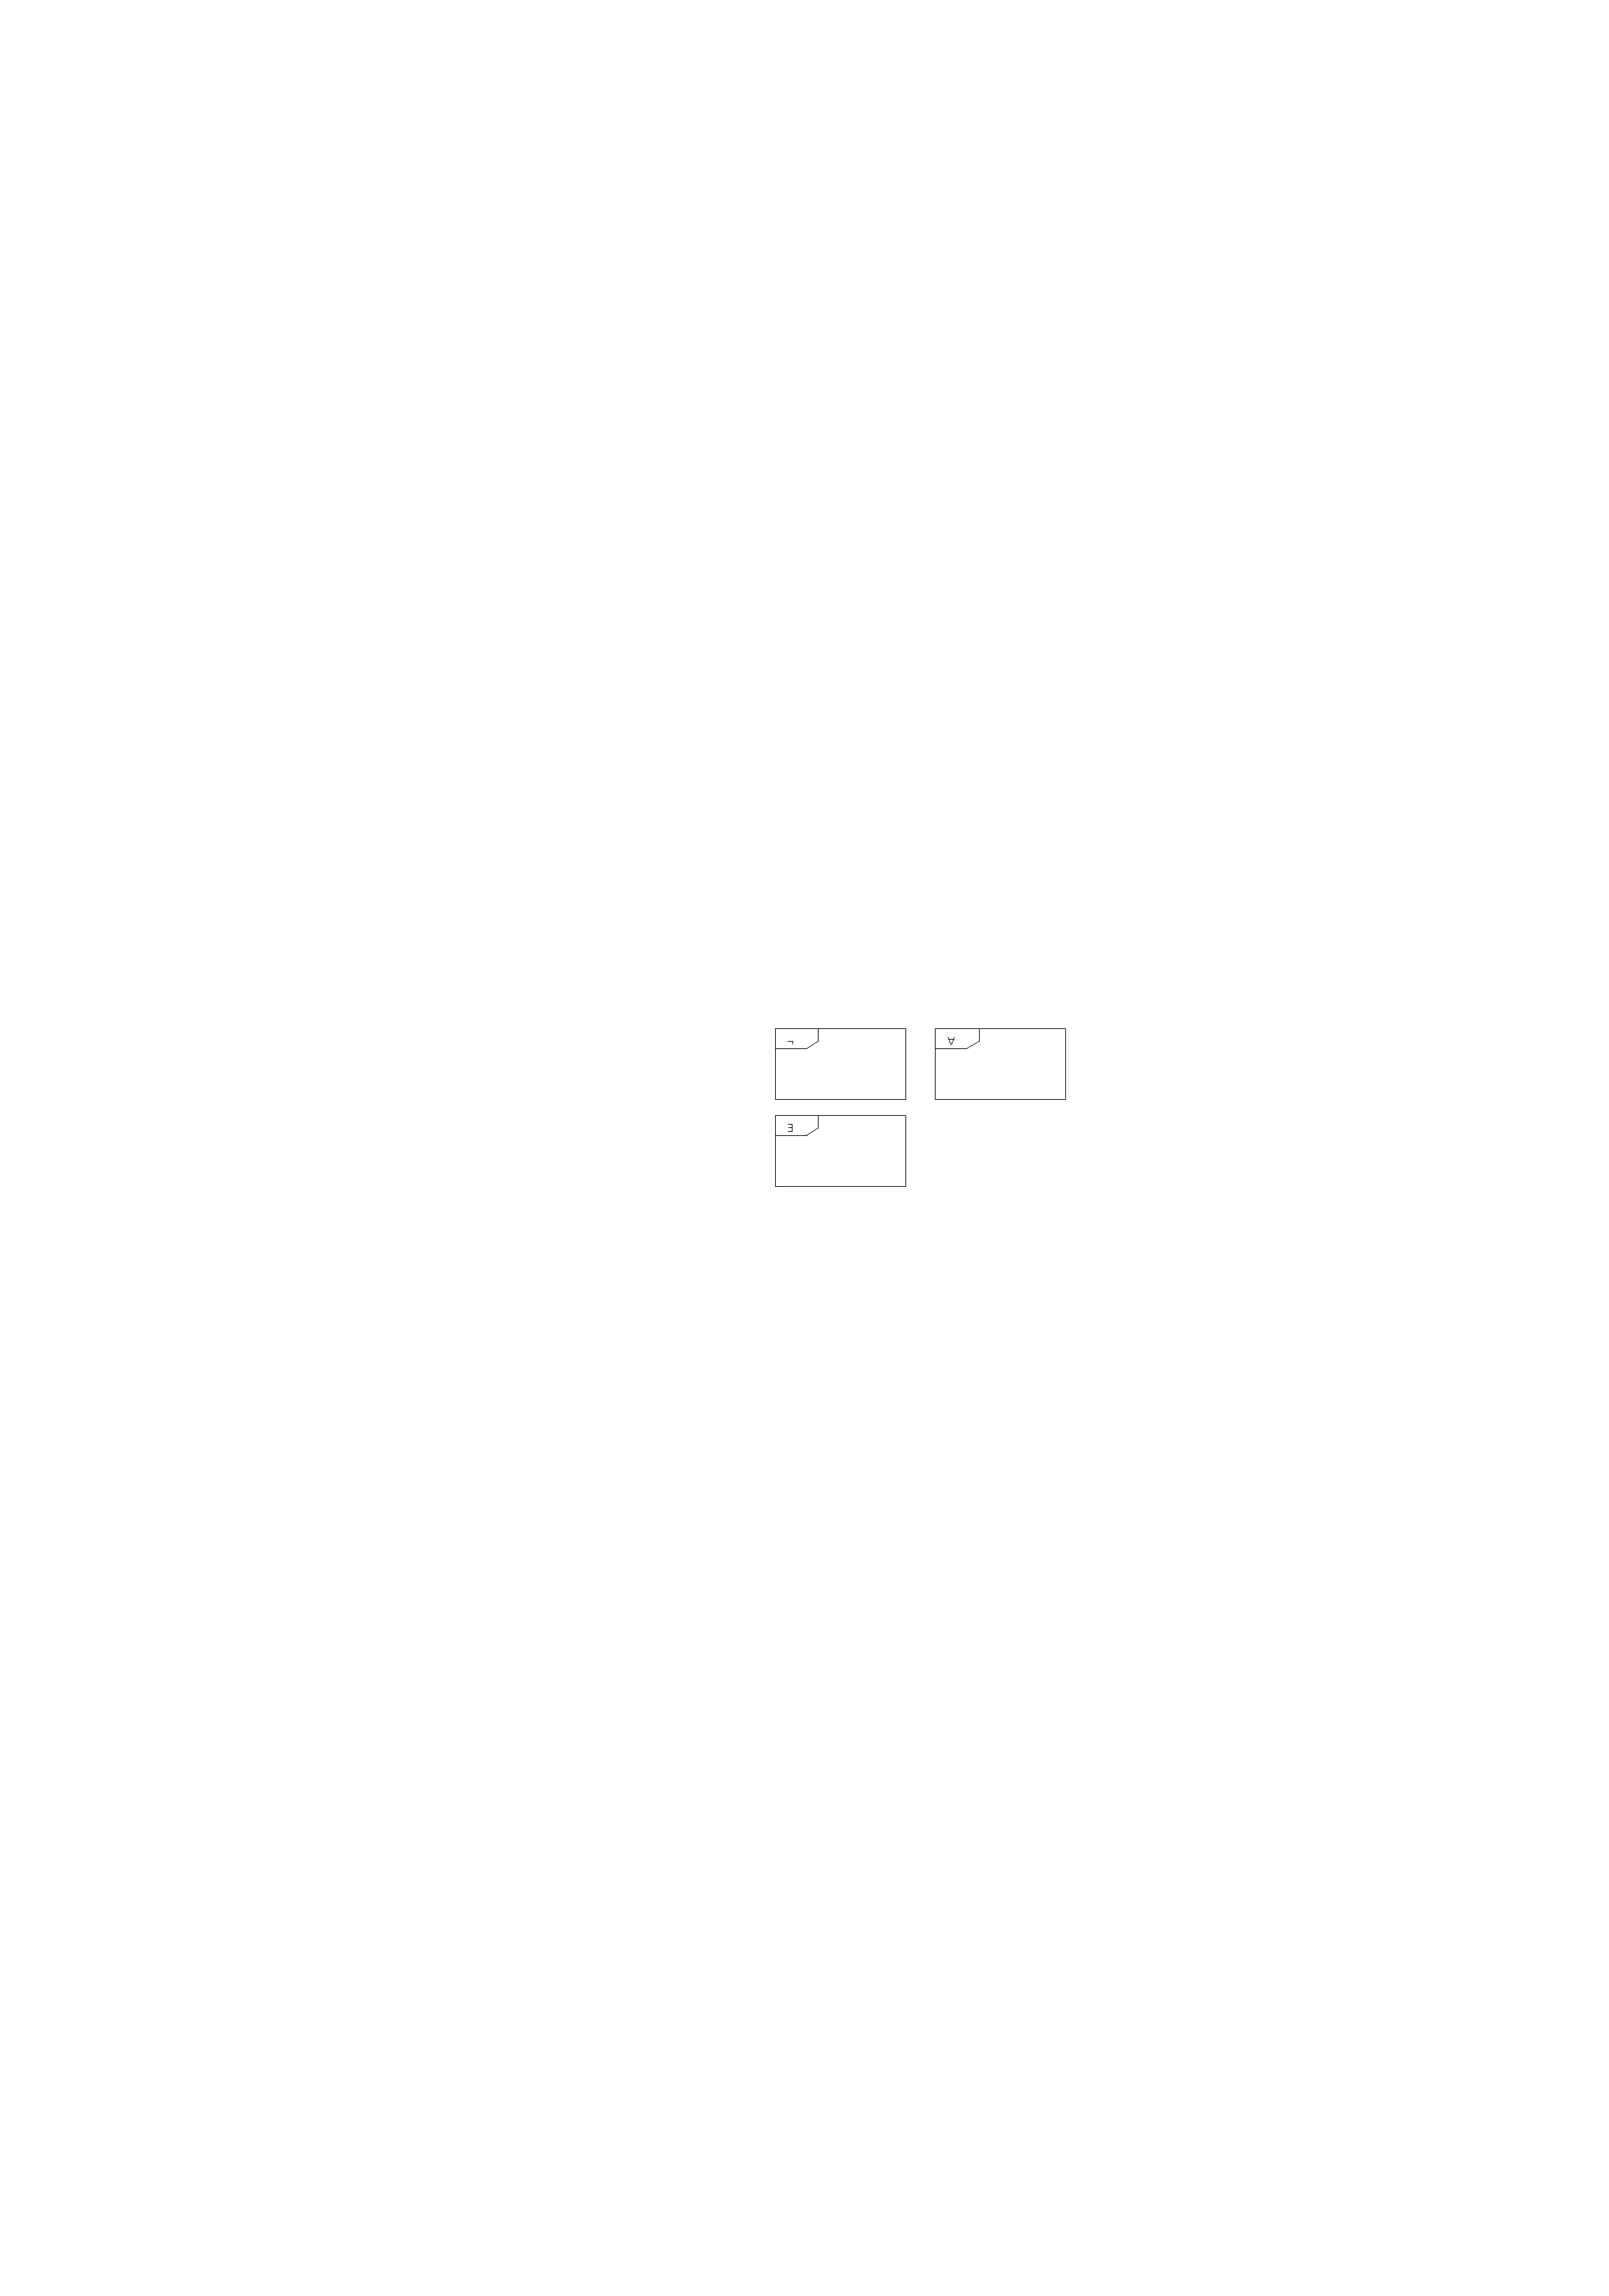
\includegraphics[scale=1.0]{figures/ContainedPattern}
  \caption{Different Kinds of Contained Patterns}
  \label{fig:containedPattern}
\end{figure}

\todomcp{Should contained pattern be marked as optional? Is currently possible in the metamodel. Idea for semantics: Whole pattern must be found, if found, variables may be used in subsequent activities, if pattern may not be found as a whole, matching still succeeds but all variables in the subpattern are not bound in subsequent activities.}
\tododt{I would say, contained patterns are mandatory in general (or are NAC/optional/set in case of the according fragment).}

\begin{figure}[htbp]
  \centering
  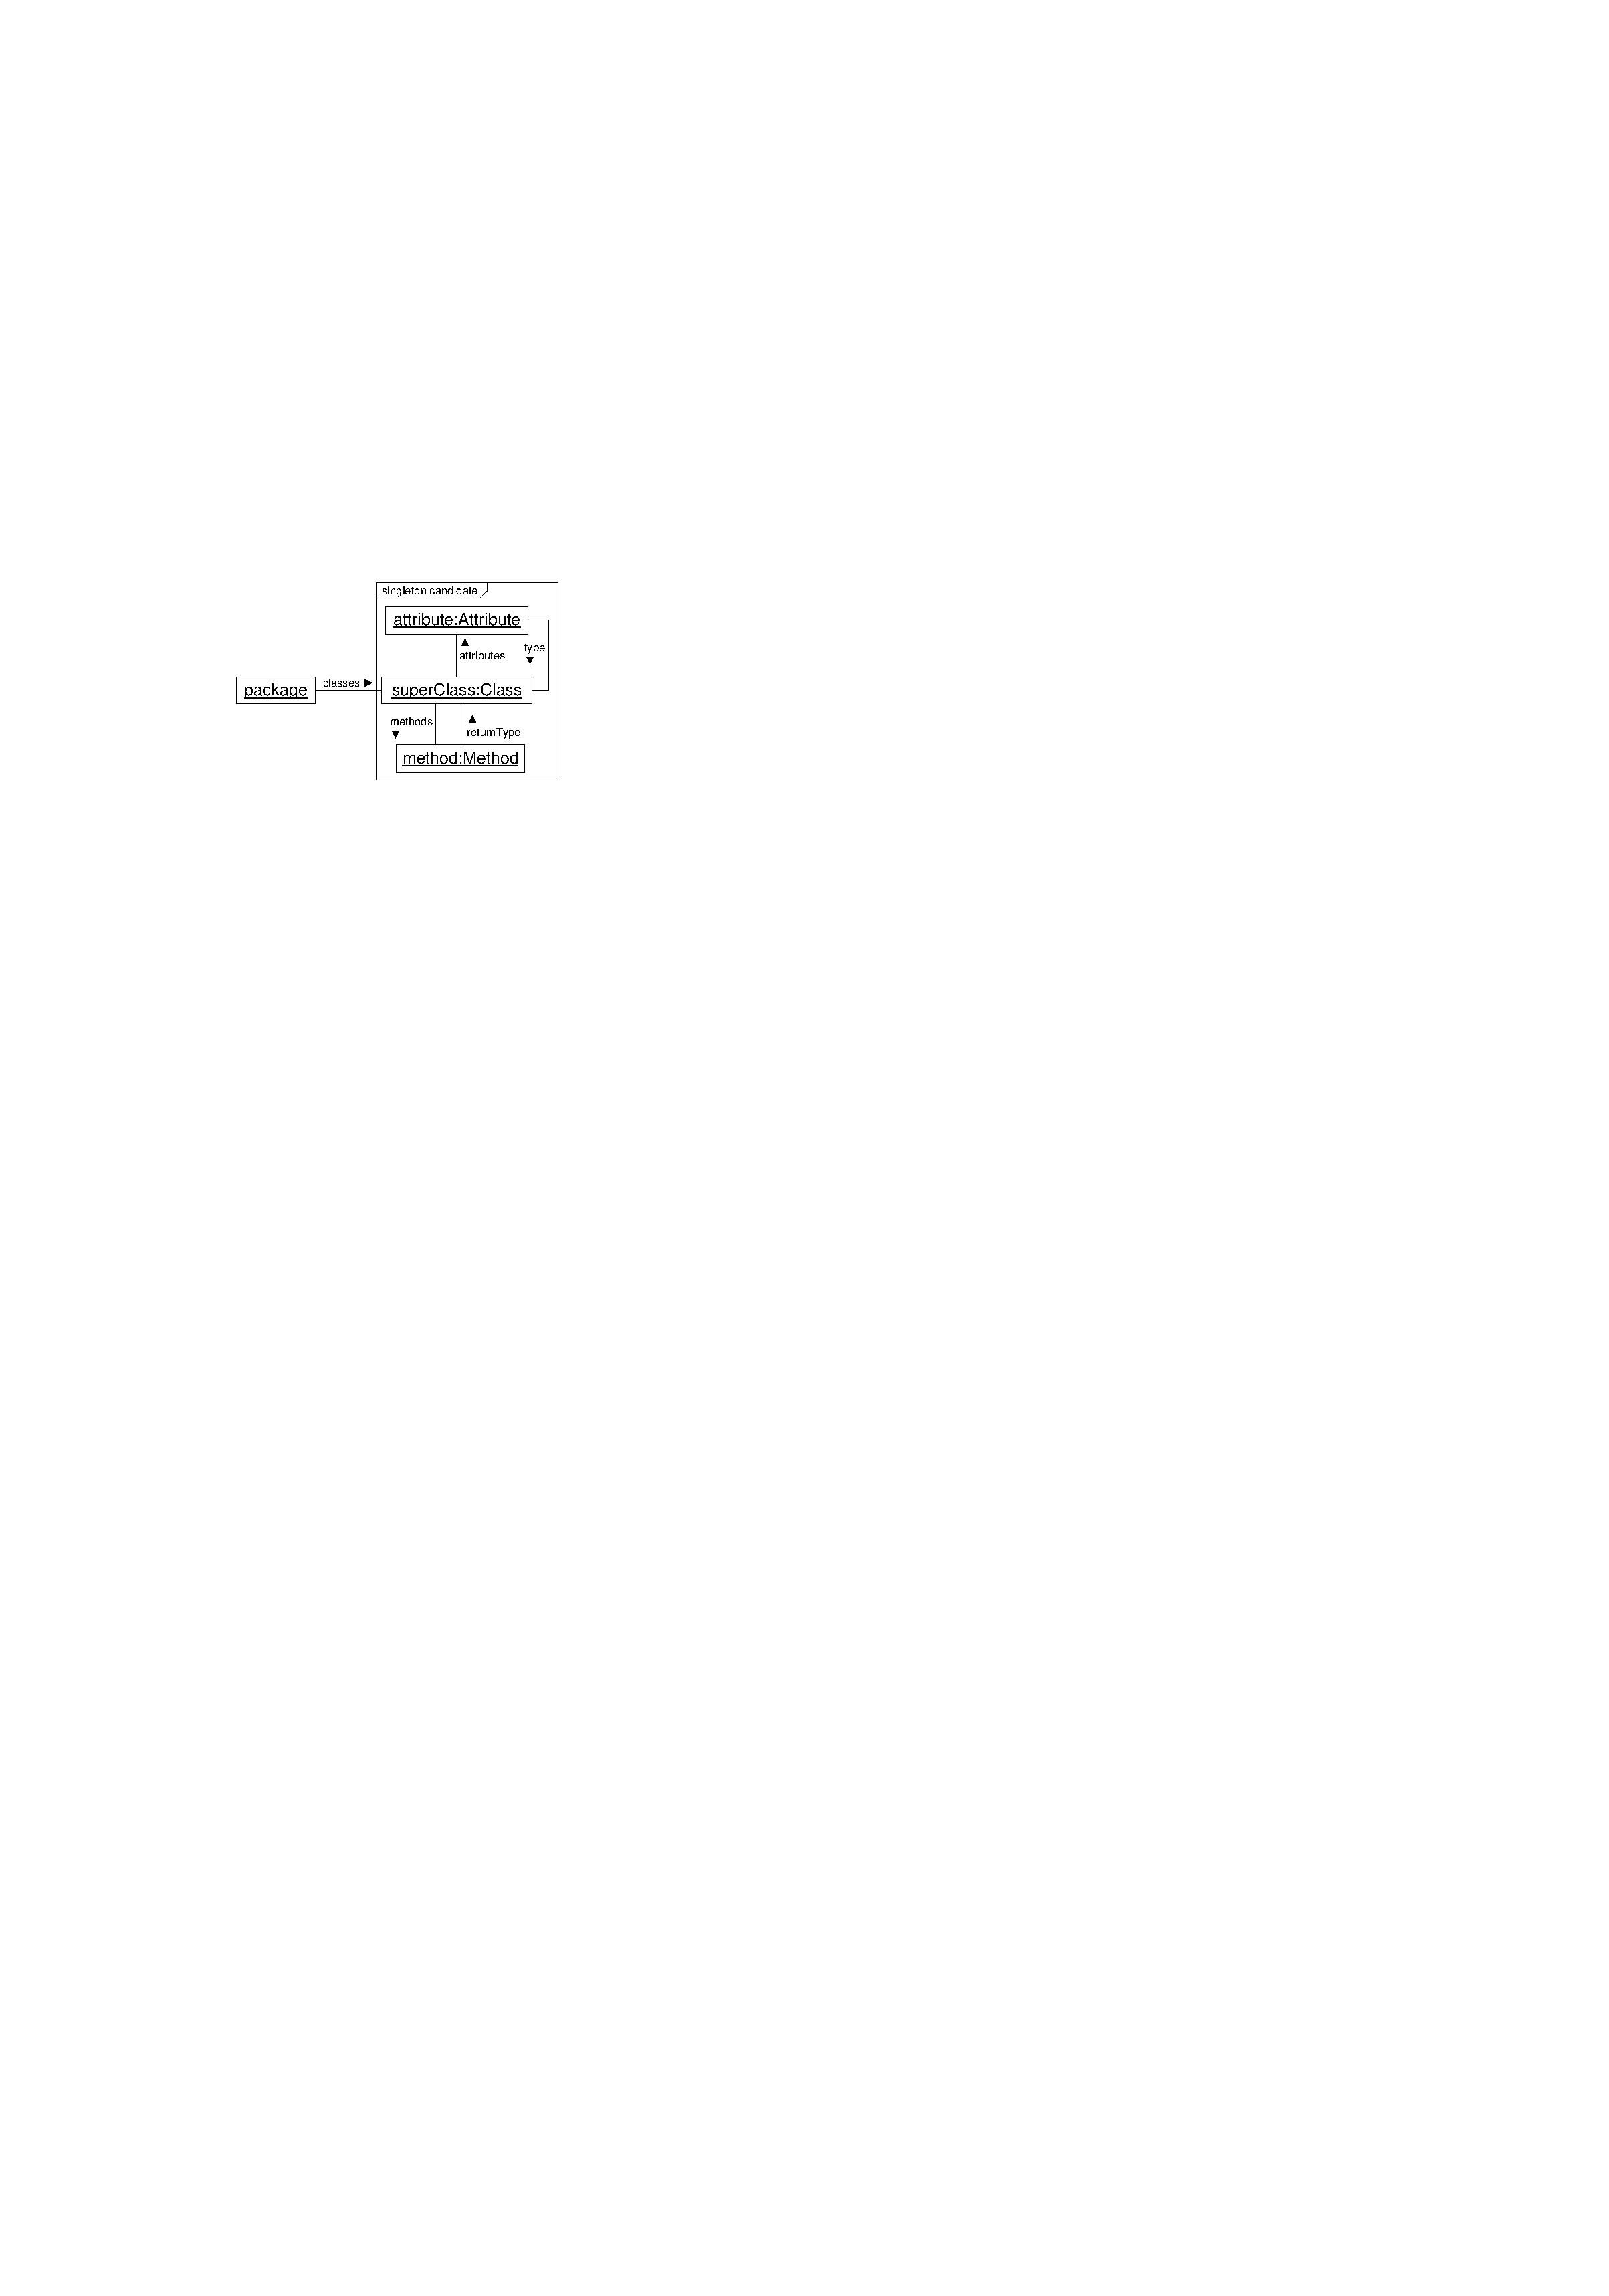
\includegraphics[scale=1.0]{figures/SubPatterns2}
  \caption{Labeled sub pattern}
  \label{fig:labeledSubPattern}
\end{figure}

\begin{figure}[htbp]
  \centering
  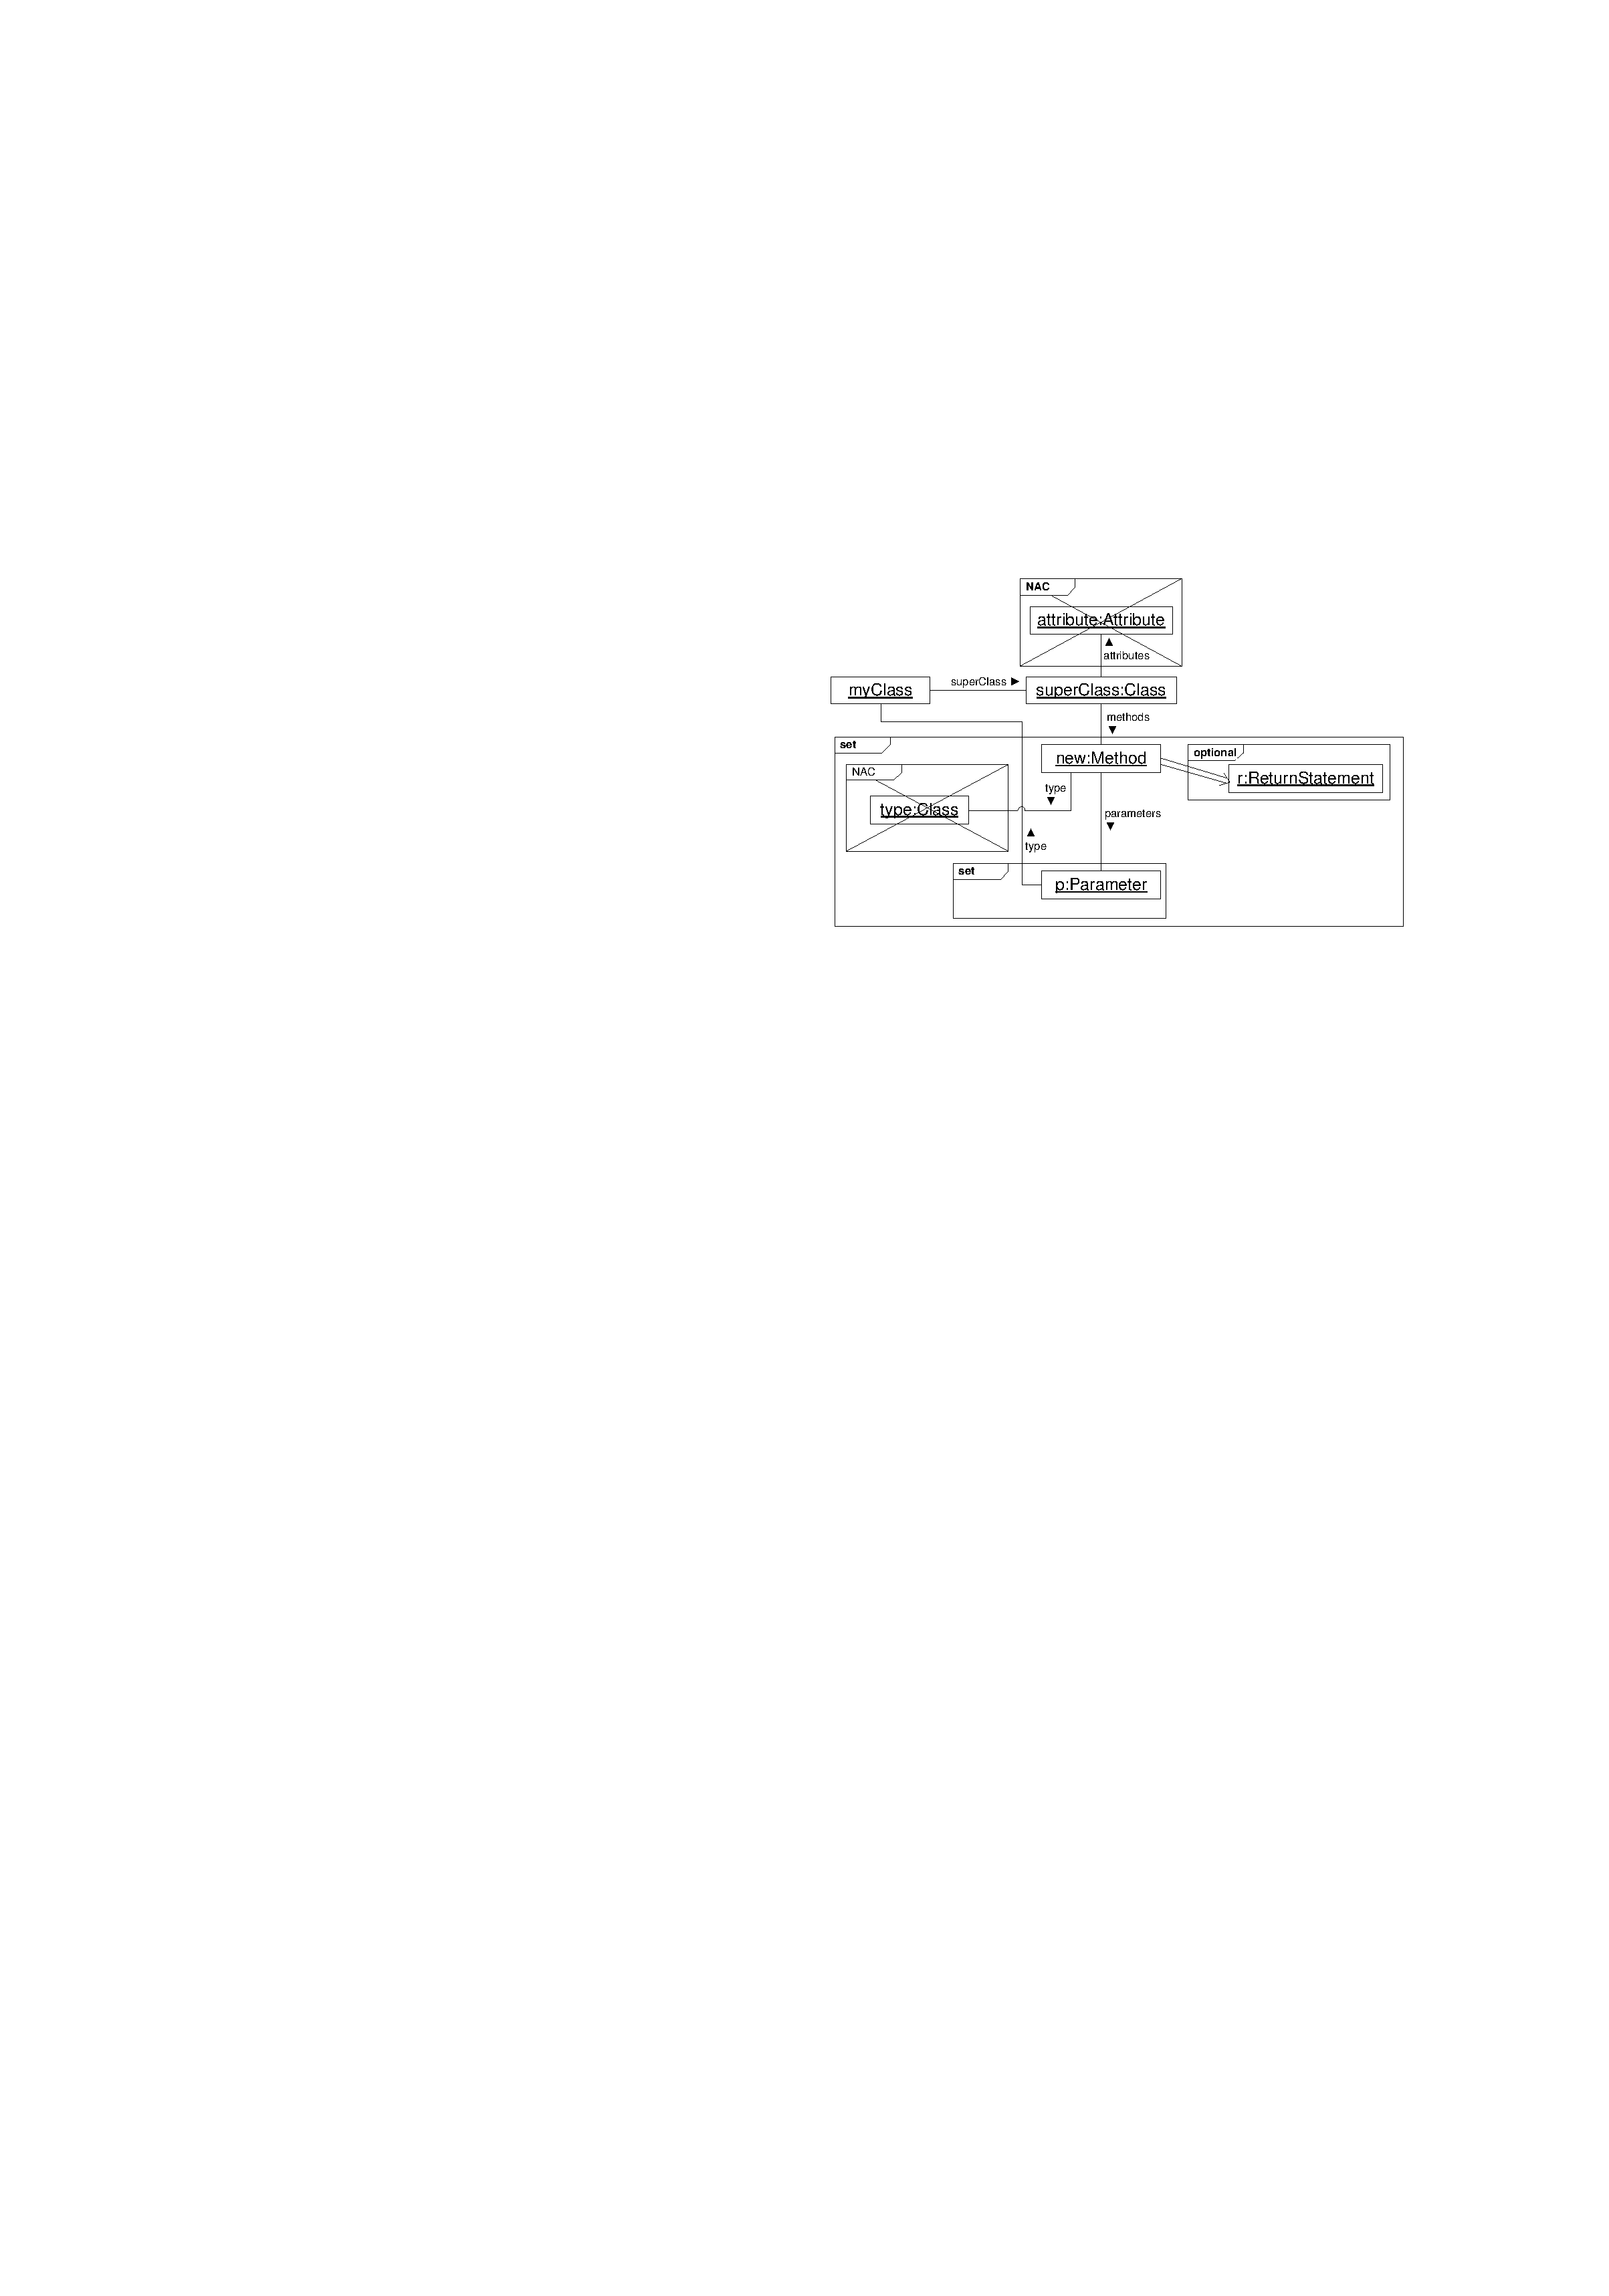
\includegraphics[scale=1.0]{figures/SubPatterns1}
  \caption{Hierarchies of NAC, set, and optional sub patterns}
  \label{fig:subPatternHierarchies}
\end{figure}

\todomcp{How deep may patterns be nested? What is the semantics of alternating binding semantics of sub-patterns, e.g., negative in optional in negative and so on.}
\tododt{I would prefer to allow arbitrarily deep nestings and would suggest to interpret the fragments in the order from outside to inside. Example (see Figure~\ref{fig:subPatternHierarchies}): You match a super class \emph{superClass} of \emph{myClass} and ensure that \emph{superClass} has no attribute. Then you you match all methods \emph{new} (outer set fragment) that have no class as their type (enclosed NAC fragment). Now you match for each of these methods all parameters (enclosed set fragment) that have \emph{myClass} as their type. Furthermore, you try to find a path from the matched \emph{new} method to a return statement (optional fragment).}

} %--- End of pattern fragment section


 
	
	\section{Story Diagrams} \label{sec:StoryDiagrams}

After explaining the concept of story patterns in Section~\ref{sec:StoryPatterns}, a prerequisite for this section, we explain the story diagrams themselves.
We give an overview of the general idea in Section~\ref{sec:IdeaStoryDiagrams} and go on with explaining the language constructs in the following sections.

\subsection{General Idea}\label{sec:IdeaStoryDiagrams}

% - combine activity diagrams and graph transformations as well as imperative, deterministic and declarative, non-deterministic languages to formally and compactly describe software behavior in terms of model transformations using an OO-based, familiar notation

The main idea behind story diagrams is to formalize UML activity diagrams
to better support model-driven software development.
This is done by not only modeling the software structure, but also completely modeling its behavior and, thus, making the software model executable.
For that purpose, graph transformations were chosen to formally specify behavior and have been combined with UML activity diagrams.
The result, story diagrams, is a mixture of two languages:
an imperative, deterministic language for the description of control flow, namely UML activity diagrams,
and a declarative, non-deterministic, object-oriented, graph-transformation-based language for the description of model modifications, so-called story patterns (see Section~\ref{sec:StoryPatterns}).
Both languages are graphical, formally defined, and use a familiar notation based on UML 1.5 activity diagrams\footnote{Actually,
we use the notation of UML 1.5 activity diagrams, but already use the terminology of the UML 2.}
and UML object diagrams with minor modifications.

An exemplary story diagram is illustrated in Figure~\ref{fig:simpleStoryDiagram}.
This story diagram takes a graph-based representation (a model of a so-called abstract syntax graph, see Section~\ref{sec:typeGraph}) of an object-oriented program, e.g., in Java,
and replaces calls of a given method (\fe{oldMethod}) with calls of another given method (\fe{newMethod}).

\begin{figure}[htb]
  \centering
  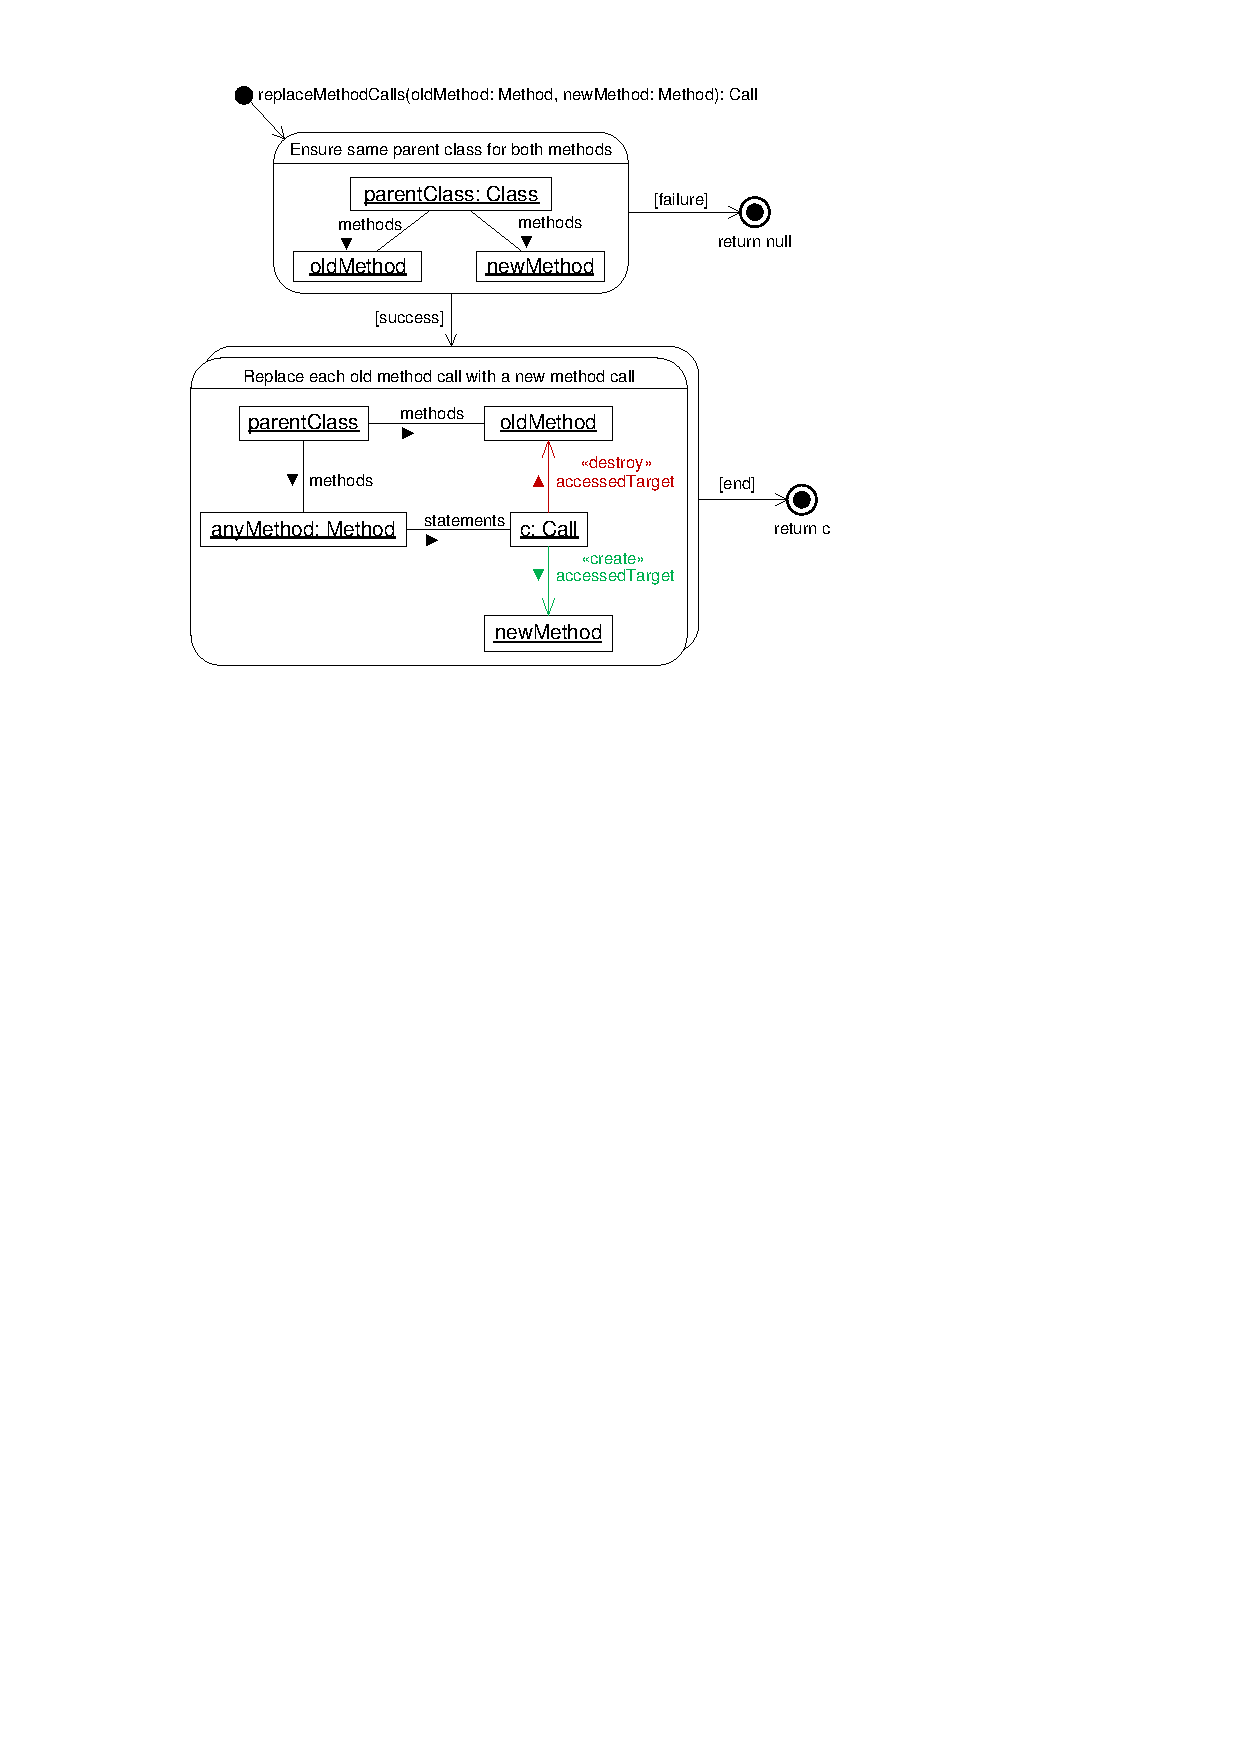
\includegraphics[scale=1.0]{figures/SimpleStoryDiagramExample}
  \caption{Exemplary Story Diagram -- Replace Method Calls}
  \label{fig:simpleStoryDiagram}
\end{figure}

Like UML activity diagrams, story diagrams model control flow by means of activity nodes and activity edges.
Each activity node embeds a story pattern to formally specify the behavior for this node\footnote{There are
some exceptions like activity call nodes which do not contain story patterns to specify the behavior.}.
The activity edges can carry guards.
These are either specified by boolean expressions, e.g., checking attribute values of a matched object,
or by keywords used to specify decisions on whether a story pattern could be
matched or not\footnote{A story pattern is successfully matched if for each object and link variable in the pattern corresponding objects and links are found in the instance model (host graph) and all specified constraints are satisfied.}.
In Figure~\ref{fig:simpleStoryDiagram}, the used guards are \fe{\text[success\text]} (successful execution of a story pattern),
\fe{\text[failure\text]} (failed to completely execute a story pattern),
and \fe{\text[end\text]} (activity edge points to the first activity node to be executed after a loop).

In contrast to ordinary UML activity diagrams, story diagrams, so far, do not model concurrent execution.
Thus, the language constructs \emph{fork} and \emph{join} are currently not supported in story diagrams.
We plan to include these concepts in future versions of story diagrams.

%- Story diagrams in MDSD process, 2 worlds: stand-alone transformations and specifications of methods' behavior:
%  1. alternative (completely modeling software): model classes in class diagrams, specify their methods' behavior in story diagrams, generate executable source code (e.g. Java) or use an interpreter
%  2. alternative (specify recurring model operations/transformations for a given type of models): model only classes representing the editor's model under development (meta-model), specify modification operations of this model (adding and removing elements, analysis operations, translations to/generation of other models, etc.), need of a software that triggers the specified operations, the operations can be performed using generated code or an interpreter
%- introduce an example

Basically, there are two different ways of using story diagrams in a model-driven software development process.

Originally, story diagrams were used in object-oriented software development to formally specify the behavior of methods that are defined in classes.
Calling such a method means to execute the story diagram that represents the method's behavior.
If there is a story diagram that models the behavior for each method specified in a class model,
the software model completely covers the software's structure and behavior and, thus, can be analyzed and executed.
In this case, story diagrams specify the behavior of objects whose properties are defined by classes.
For that reason, those story diagrams have a \emph{this} variable -- similar to the keyword \emph{this} in Java -- representing the object (a class instance) that they belong to (a self reference).
This variable can be used as a starting point for the graph matching specified in a story diagram.

For example, the class diagram in Figure~\ref{fig:SDWithThisClassDiagram} defines a method \fe{findAttribute} for all \fe{Class} objects.
This method's behavior is specified by the story diagram in Figure~\ref{fig:SDWithThis}.
The matching of the object structure specified in the contained story pattern, in this case,
starts with the \fe{this} object variable of the type \fe{Class} which is already bound
to the \fe{Class} object that the \fe{findAttribute} method belongs to.
Thus, this method tries to find an attribute \fe{a} in the same class with the name given by the method's parameter \fe{text}.

\begin{figure}[htb]
	\centering
  \begin{minipage}[t]{.4\textwidth}
    \centering
    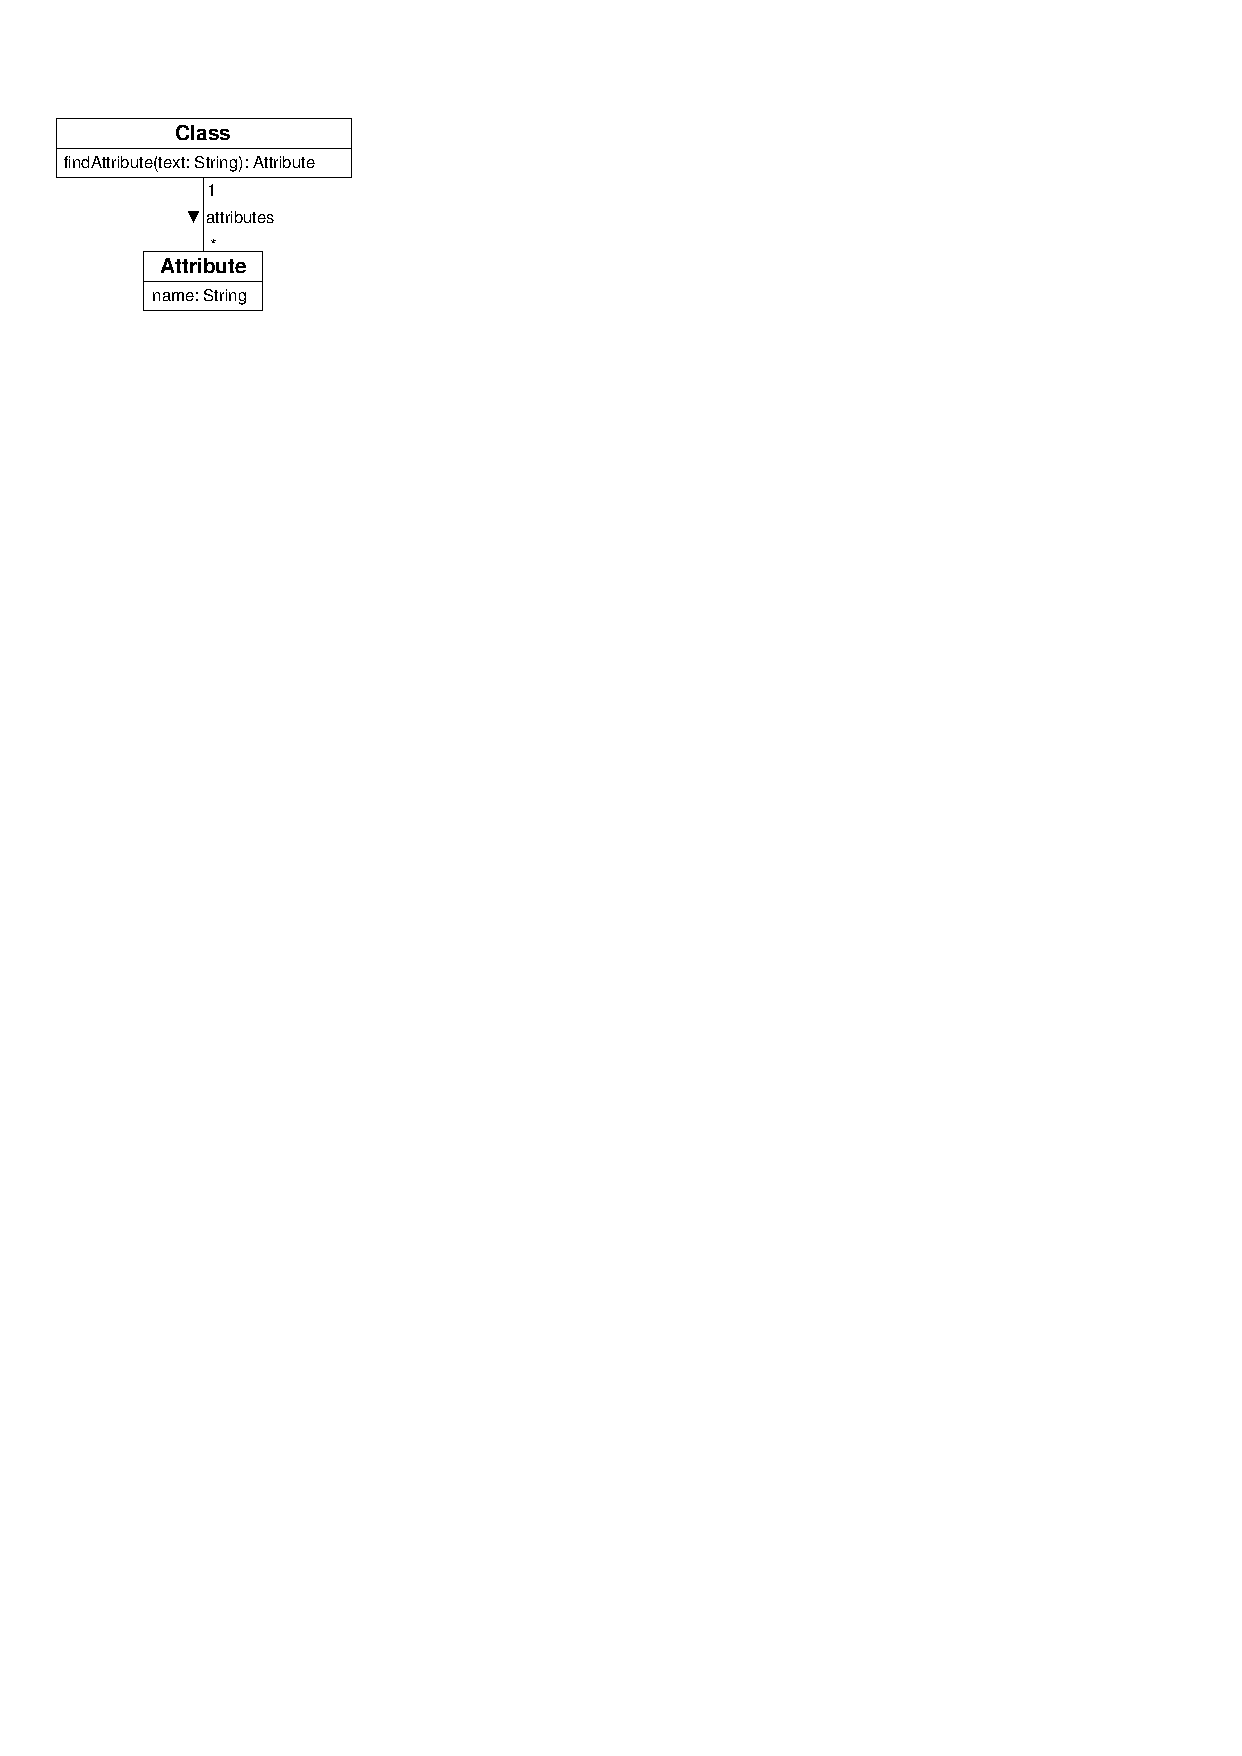
\includegraphics[scale=1]{SimpleSDFindAttributeClassDiagram} 
    \caption{Type Model for the Story Diagram in Figure~\ref{fig:SDWithThis}}
    \label{fig:SDWithThisClassDiagram}
  \end{minipage}%
  \hfill
  \begin{minipage}[t]{.55\textwidth}
    \centering
    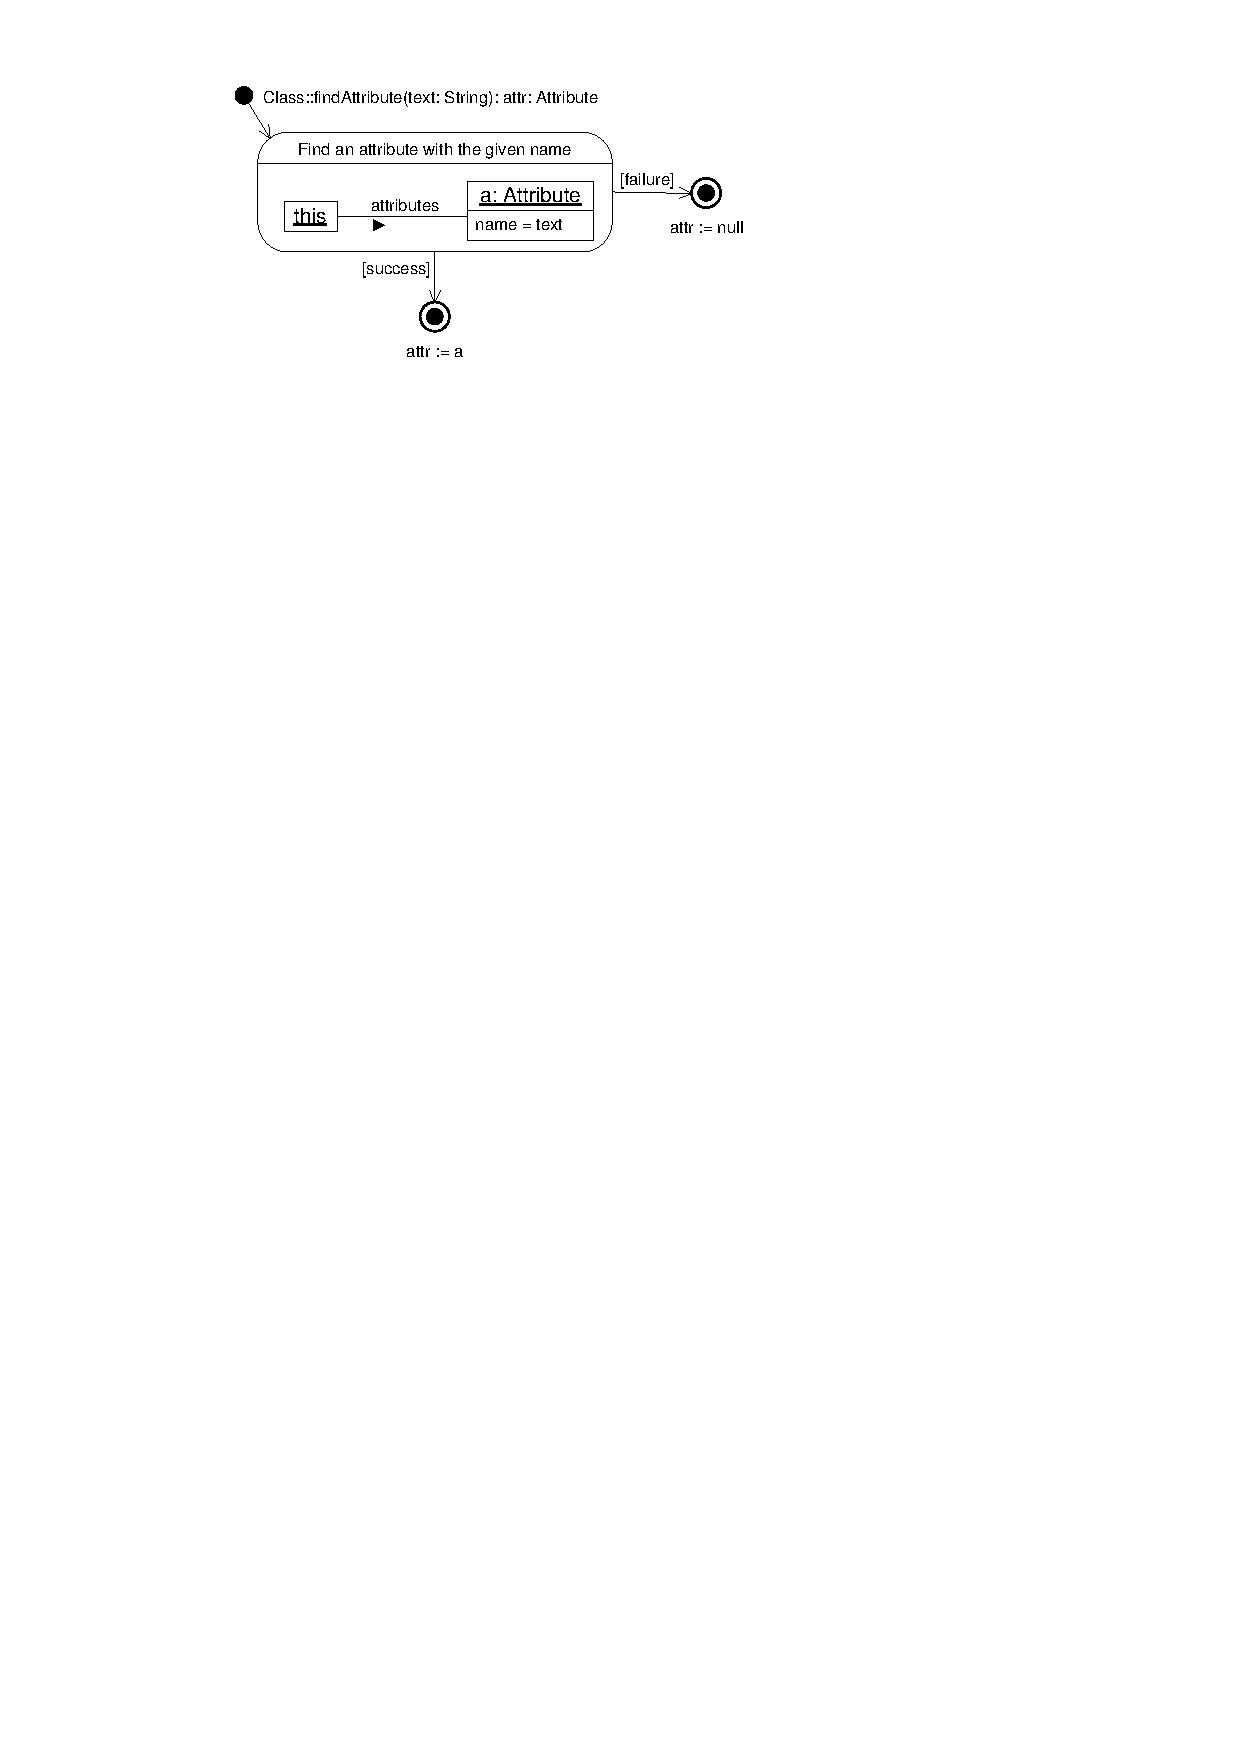
\includegraphics[scale=1]{SimpleSDFindAttribute}
    \caption{Exemplary Story Diagram With \emph{this} Object Variable}
    \label{fig:SDWithThis}
  \end{minipage}
\end{figure}

\begin{figure}[htb]
	\centering
  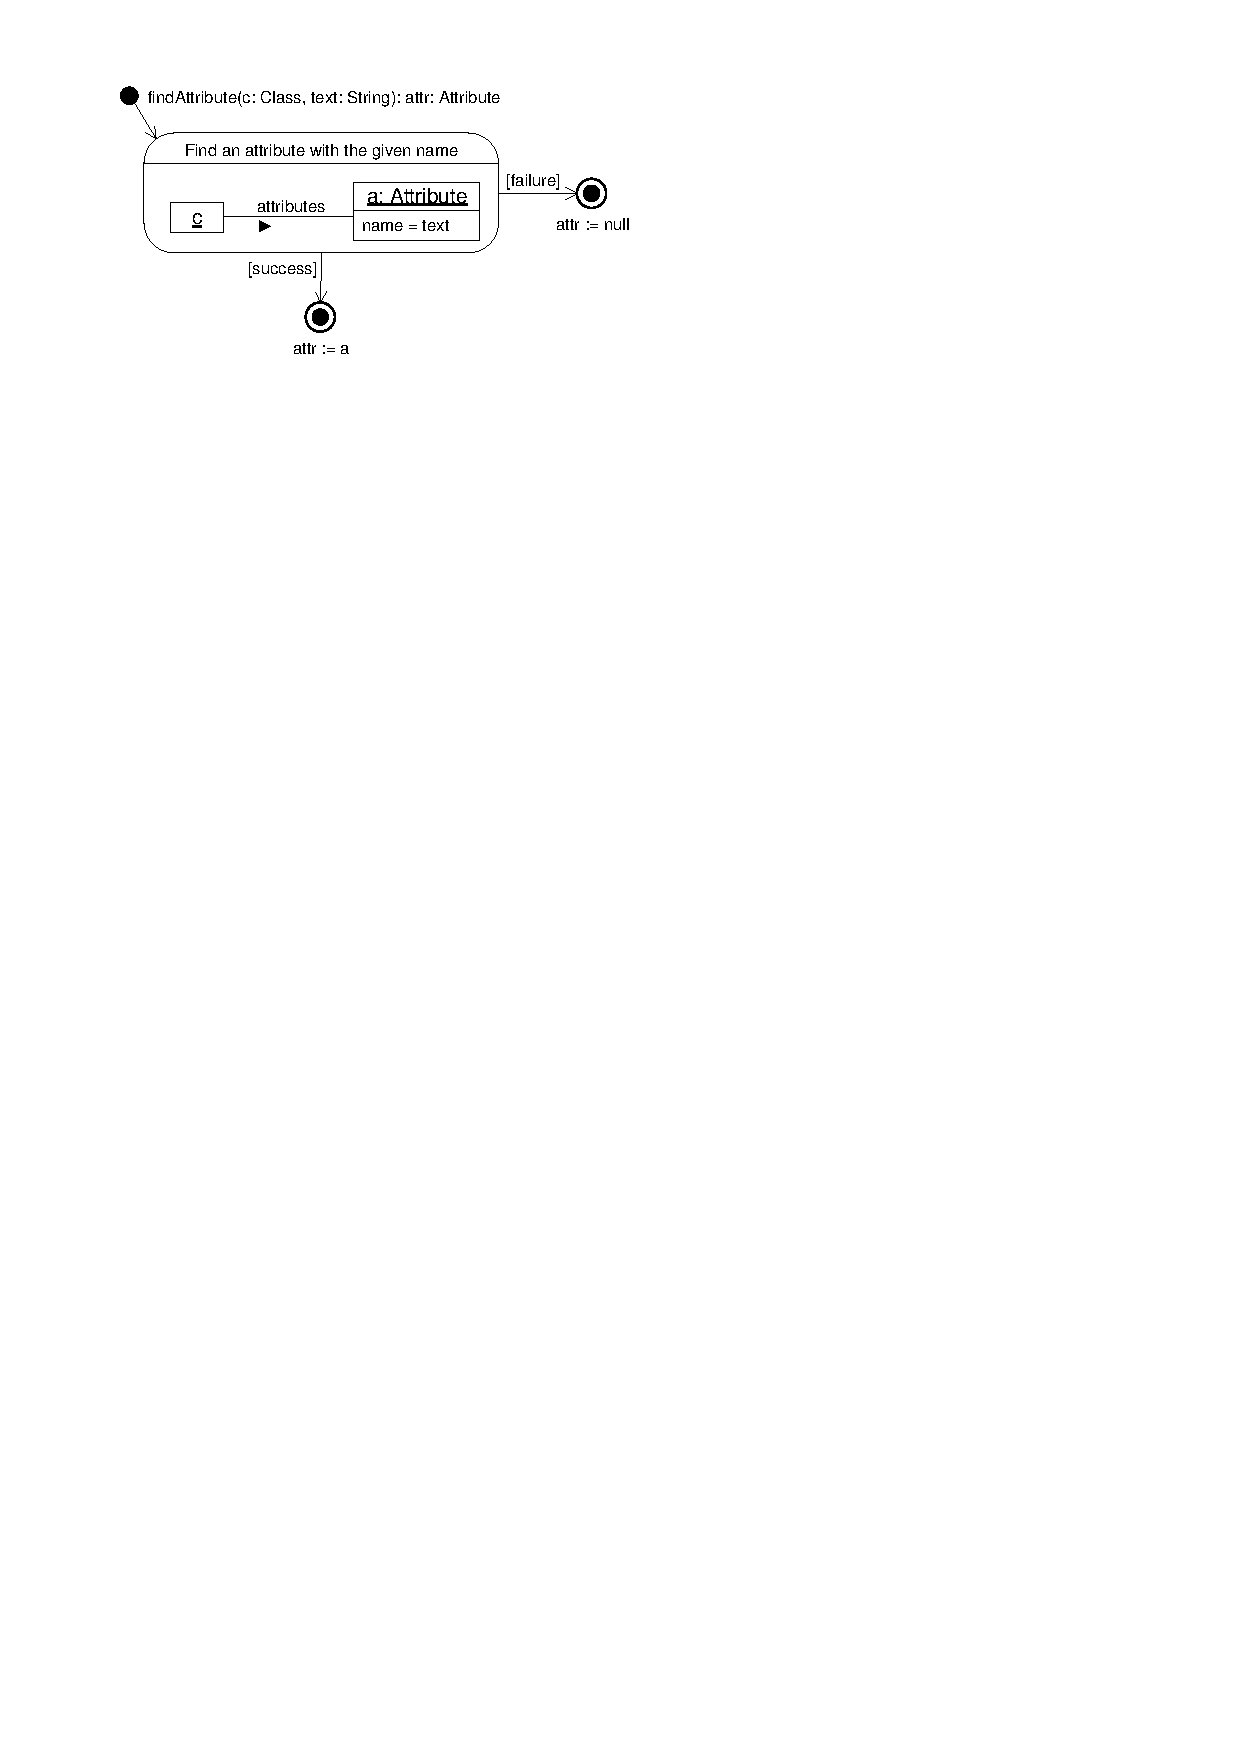
\includegraphics[scale=1]{SimpleSDFindAttributeStatic} 
  \caption{Exemplary Story Diagram Without \emph{this} Object Variable}
  \label{fig:SDWithThisStatic}
\end{figure}

Another more flexible way of using story diagrams is to specify any kind of model transformation or operation in a story diagram without attaching this behavior to a certain class.
In contrast to the previous case, there is no \emph{this} variable that could be used as a starting point for the graph matching.
All starting nodes for the graph matching have to be provided as arguments of the story diagram call.
For this purpose, in contrast to the story diagram in Figure~\ref{fig:SDWithThis}, the story diagram in Figure~\ref{fig:SDWithThisStatic} has an additional parameter \fe{c}.
The corresponding arguments of a story diagram call are assumed to be known (bound object variables) and are used as starting points for the graph matching.
This way, the operations or transformations defined by story diagrams can be used from within any other part of the developed software, like a software library would be used.
Typically, model-to-model transformations, consistency checks, or more generally speaking, recurring and object-independent operations are defined this way.

% - enable formal analyses to check/ensure certain behavioral software properties

In both cases, story diagrams can be used to generate executable source code or be executed using an interpreter.
Besides execution, the formally defined story diagrams can also be analyzed to guarantee certain behavioral properties \cite{Mey09,Zue09}.
For example, model checking can be used to check whether a certain invariant holds
(e.g.\ that all accessible variables are still accessible after a refactoring operation)
or if a critical state can ever be reached (e.g.\ if an attribute or method has no parent class after a refactoring operation which would result in an incorrect program).

A complete description of the story diagrams' abstract syntax is given in the Appendix~\ref{sec-reference}.
There is also a grammar that determines all feasible story diagrams by constraining their structure.
The latest version of this grammar can be found in Thomas Klein's diploma thesis \cite{Kle99}.


%\subsection{The Language Constructs in Story Diagrams (Jan/Dietrich)}\label{sec:StoryDiagrams:composition}

\subsection{Activities, Activity Parameters and Return Values}\label{sec:activities}

Since story diagrams can be seen as special UML activity diagrams, we reused the class names defined by the UML 2.
Thus, similar to UML activity diagrams, a story diagram is represented by a so-called activity (class \fe{Activity}).

Each story diagram can have parameters.
We distinguish \emph{in} and \emph{out} parameters,
i.e.\ parameters representing arguments given when a story diagram is called (\emph{in})
and parameters representing return values (\emph{out}).
Parameters are either \emph{in} or \emph{out} parameters.
%Parameters can be \emph{in} and \emph{out} parameters at the same time.
The story diagram in Figure~\ref{fig:SDWithThisStatic} has two \emph{in} parameters \fe{c} and \fe{text}
as well as an \emph{out} parameter \fe{attr} of the type \fe{Attribute}.
If there are more than one \emph{out} parameter, these are comma-separated.

If a story diagram defines the behavior of a method, the parameters are defined by the corresponding method's signature.
In this case, the number of \emph{out} parameters is limited to one single parameter and represents the only \emph{return} value of the method and story diagram.
Besides these parameters, there is another implicitly defined parameter \fe{this}
which -- similar to Java's \fe{this} keyword -- represents the object that the story diagram belongs to.

In case a story diagram is not defining a method's behavior, it defines its own signature explicitly with according \emph{in} and \emph{out} parameters.
The number of \emph{out} parameters is allowed to be arbitrary in this case and there is no \emph{this} parameter.

The values or objects returned after execution of a story diagram are defined by expressions in the \emph{stop} activity nodes.
For example, the object matched to the object variable \fe{a} is returned by the story diagram in Figure~\ref{fig:SDWithThisStatic} in case of a successful execution.
This is specified by the expression \fe{attr := a} which represents an assignment of the value of object variable \fe{a} to the \emph{out} parameter \fe{attr}.
Otherwise, an empty reference is returned which is specified by the keyword \fe{null}.
This notation is taken from Matthias Meyer \cite{Mey09}.

\subsection{Activity Nodes, Activity Edges} 
\label{sec:storydiagrams:activitynodes}

A story diagram's control flow is defined by activity nodes and activity edges, similar to UML activities.
Except for the cases where an activity node represents a call of another story diagram,
each node embeds a story pattern to specify the corresponding behavior.
Such activity nodes are called \emph{story nodes}.
Executing a story node results in executing the embedded story pattern.

In contrast to single story patterns, story patterns contained in story nodes of a story diagram have a different scope.
Here, you can reuse all object variables declared in the story patterns of preceding story nodes.
For example, in Figure~\ref{fig:simpleStoryDiagram} (p.~\pageref{fig:simpleStoryDiagram}),
the object variable \fe{parentClass} is reused in the second story pattern
by specifying the variable as a bound variable, i.e.\ the variable does not have to be matched anymore.

Executing a story node means executing the corresponding story pattern
which, in turn, means finding a subgraph with the specified properties
(e.g.\ finding objects of a certain type, with certain attribute values, and with certain connections)
and performing specified modifications of the found subgraph
(e.g.\ creating or removing objects and links or changing their attribute values).

We distinguish two kinds of story nodes: \emph{modifying story nodes} and \emph{matching story nodes}.
A matching story node contains a story pattern that only matches a specified object structure, but does not change it.
A modifying story node also performs modifications of the matched object structure.
For static analyses of model transformations described with story diagrams,
it is helpful to know which transformations do not modify the instance model.

\subsection{Activity Final Nodes} \label{sec:StopNodes}

The application of a story diagram can succeed or fail.
Usually, when the matchings are successful and the specified transformations can be carried out, the story diagram is considered to be applied successfully.
When a matching is unsuccessful somewhere or something unforeseen happens and the application has to be aborted, the story diagram's application is considered to have failed.
This is comparable to a method call either returning a desired result or returning false or null if something goes wrong.

\tododt{I would remove or replace this first paragraph.
In my opinion, the success and failure of story diagrams are not necessarily dependent on the success or failure of some pattern matchings or transformations in the same story diagram.
In Figure~\ref{fig:successAndFailureStopNodes} one could also model that the story diagram is considered to be successfully executed if the matching in the first story pattern fails.
Thus, success or failure of a story diagram is used like an implicitly declared boolean out parameter describing if the operation described by a story diagram is considered to be successful.
In which case it is successful is specified by the developer, not by the story diagrams language.
I would point out that the success of a story diagram is not directly dependent on the successful execution of all contained story patterns.
In contrast, the success and failure of story patterns are defined by the language.}

When one story diagram calls another, the calling story diagram's further execution may depend on the called story diagram's application being successful.
For example, the calling story diagram might need a return value of the called story diagram or it may only continue in a meaningful way if the called transformation has succeeded.
Therefore, a means to express and communicate the successful or unsuccessful application of a story diagram is required.
Story diagrams have success and failure final nodes for this.

In normal UML activities, the final nodes determine where control flow of the activity ends.
Story diagrams reuse this concept but they annotate the nodes with either \emph{success} or \emph{failure}.
Figure~\ref{fig:successAndFailureStopNodes} shows and example.

\begin{figure}[htb]
\begin{center}
  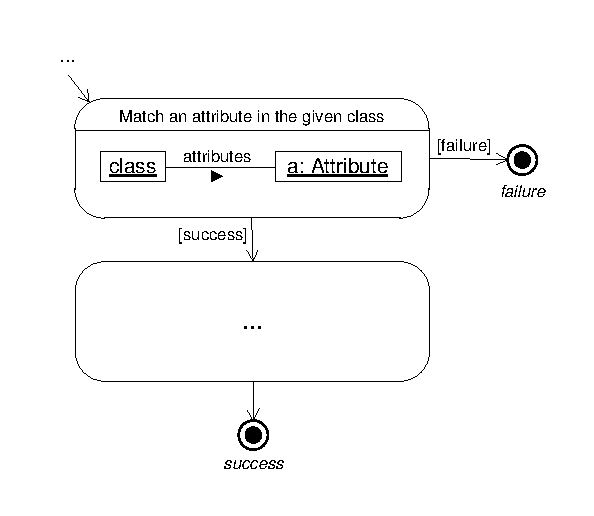
\includegraphics[width=0.7\textwidth]{figures/SuccessAndFailureStopNodes}
  \caption{Example of a success and a failure final node.}
  \label{fig:successAndFailureStopNodes}
\end{center}
\end{figure}

The upper story node in Figure~\ref{fig:successAndFailureStopNodes} specifies that an attribute of a given class object should be matched.
The failure activity edge leads to a final node also labelled with \emph{failure}.
This indicates that the application of the story diagram went wrong.

If an attribute object can be matched however, the control flow continues via the success activity edge to another story node.
Finally, it reaches a final node labelled with \emph{success}.
This indicates that the story diagram's application is considered to be successful.

While the execution of a story diagram is aborted upon reaching a failure final node, the effects of the execution up to this point are not reversed.
All modifications, e.g., object creations and deletions persist.
The developer of a story diagram has to keep this in mind when specifying a transformation.
If these side effects of failed story diagram applications are undesired, the story diagram has to be designed such that it is only aborted if no modifications already took place.
Another way would be to explicitly specify activity nodes which undo the modifications before going to the failure final node.

\todomvd{We could think about a rollback mechanism for later versions.}

\todomvd{Write something about the technical side of the propagation?}
\todoall{Modify metamodel accordingly.}

\subsection{Decision Nodes, Guards, and Loops}
\label{sec:DecisionNodesEtc}

The behavior of a story node is defined by its story pattern.
Therefore,
since trying to find a subgraph defined by a story pattern can fail,
each execution of a story node can also fail.
\tododt{Where is the meaning of failure described exactly? Should it be here or in the story patterns section?
Does success of a story pattern execution mean that there was a successful matching only, independly of the succeeding transformations,
or does it mean that the graph transformation (if available) could also be executed (was executable without contradictions, exceptions not considered)?
I think, success should include the transformation and we should, if possible, check
if a modifying story pattern can perform its modifications after a successful matching \emph{before} actually modifying the host graph
(check if all variables are matched and if there are contradictions).
Someone has to describe that in the story patterns section or here.}

To distinguish the cases of a successful story node execution and its failure,
the outgoing activity edges can be provided with the guards \fe{\text[success\text]} and \fe{\text[failure\text]} (see Figure~\ref{fig:SD-decisions} a)).
The control flow is following the activity edge with the \emph{success} guard in case of a successful story node execution,
i.e.\ a successful matching of the corresponding story pattern.
Otherwise it follows the activity edge with the \emph{failure} guard.
If an outgoing activity edge has no guard, it covers both cases, success and failure.
The guards \fe{\text[success\text]} and \fe{\text[failure\text]} can only be used pair-wise (exactly two outgoing activity edges with exactly these two guards).
The first story node in Figure~\ref{fig:simpleStoryDiagram} (p.~\pageref{fig:simpleStoryDiagram}), for example, uses these guards.

\begin{figure}[htb]
	\centering
  \begin{minipage}[t]{.5\textwidth}
    \centering
    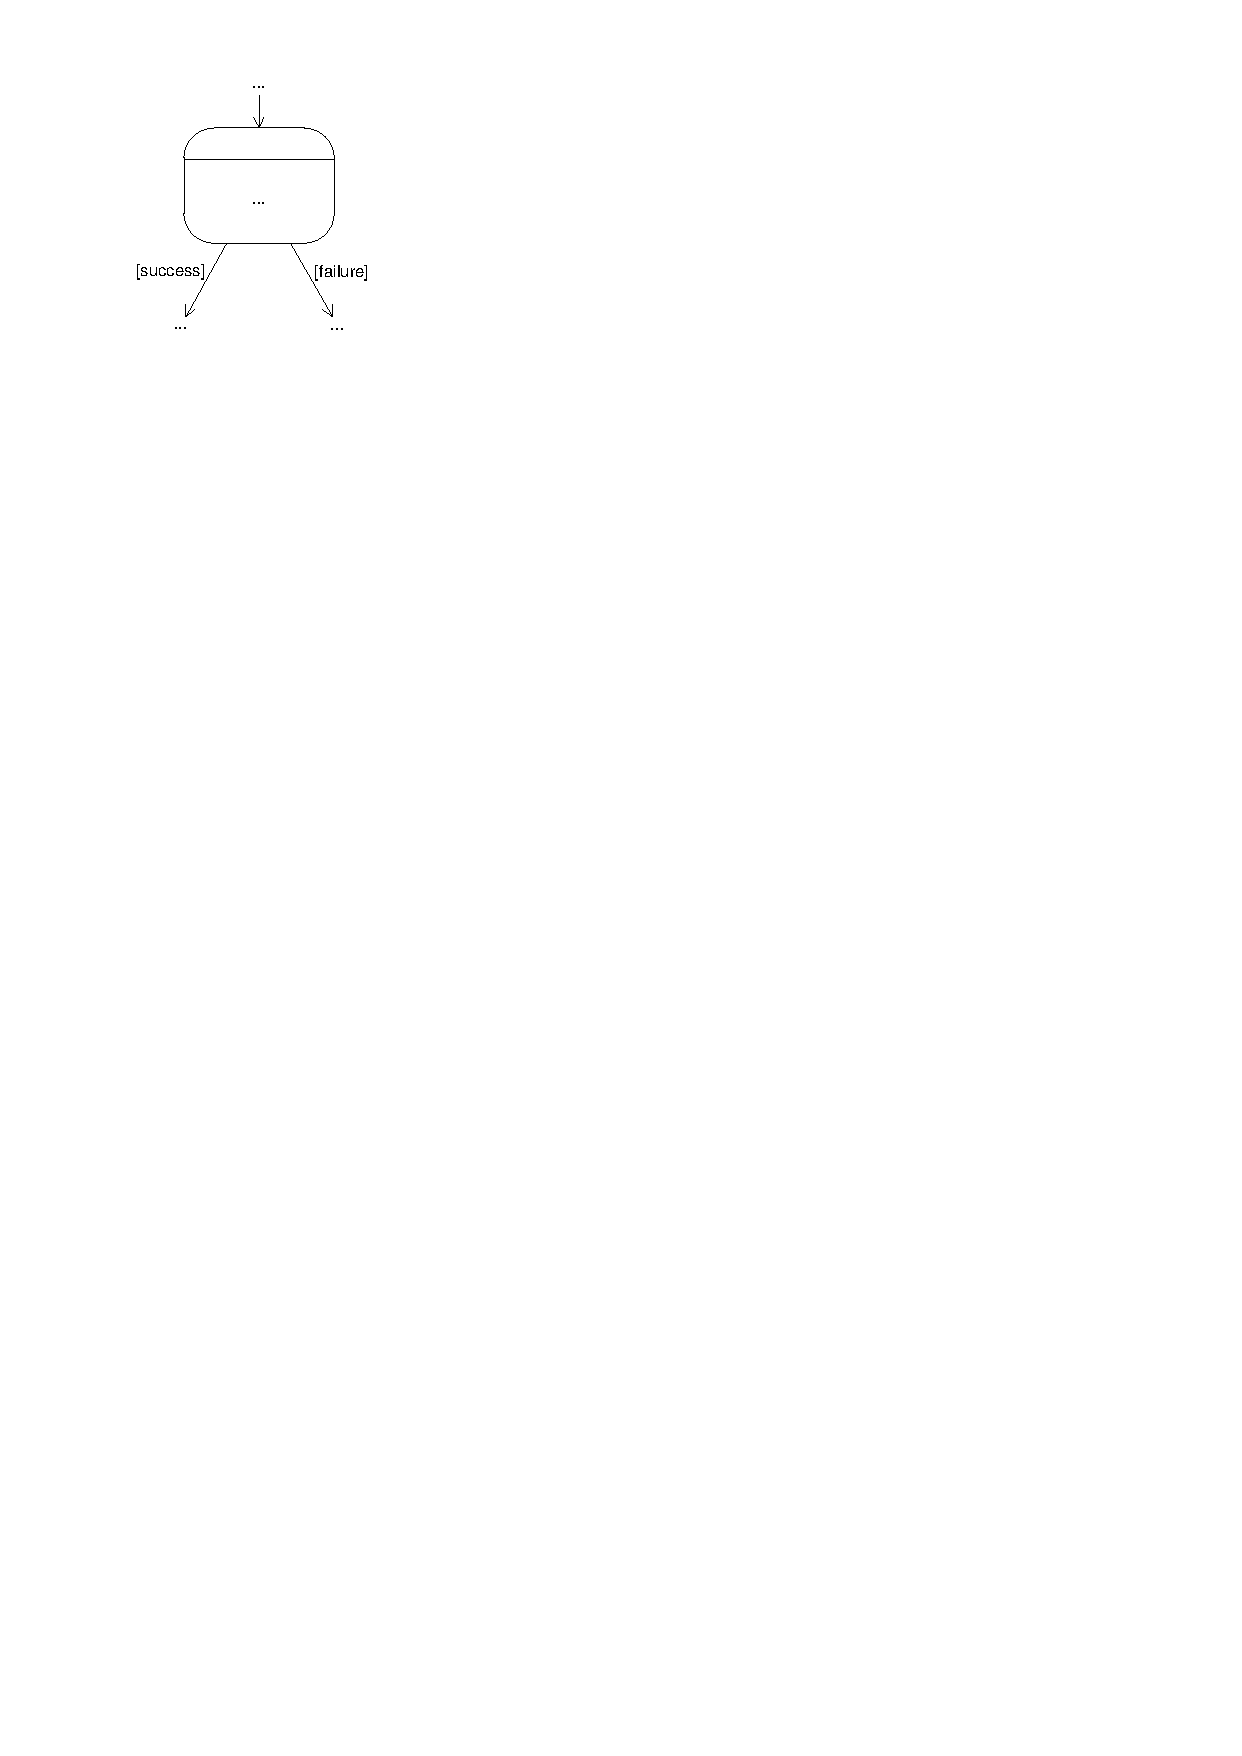
\includegraphics[scale=1]{SD-decision1}
    \\a)
    %\caption{a) Matching-Dependent Decision}
    %\label{fig:SD-decision-success}
  \end{minipage}%
  \hfill
  \begin{minipage}[t]{.5\textwidth}
    \centering
    \includegraphics[scale=1]{SD-decision3}
    \\b)
    %\caption{b) Decision Node}
    %\label{fig:SD-decision-boolean}
  \end{minipage}
%  \hfill
%  \begin{minipage}[t]{.3\textwidth}
%    \centering
%    \includegraphics[scale=1]{SD-decision2}
%    \\c)
%    %\caption{c) Boolean Conditions}
%    %\label{fig:SD-decision-nodes}
%  \end{minipage}
  \caption{Examples For Decisions}
  \label{fig:SD-decisions}
\end{figure}

Besides \fe{\text[success\text]} and \fe{\text[failure\text]}, boolean expressions can be used as guards (see Figure~\ref{fig:SD-decisions} b)).
We use the \emph{junction node} -- depicted as a diamond -- for decisions that do not depend on a previous story node.
In this case, the boolean expression of the outgoing activity edge is evaluated to \emph{true} or \emph{false}.
There can be arbitrarily many outgoing activity edges with boolean guard expressions.
The boolean expressions have to mutually exclude each other
and the corresponding guards have to be combined with an outgoing activity edge with the guard \fe{\text[else\text]}.
I.e., if there is a guard with a boolean expression, there is also an activity edge with the guard \fe{\text[else\text]}.

\begin{figure}[htb]
	\centering
  \begin{minipage}[t]{.24\textwidth}
    \centering
    \includegraphics[scale=0.9]{SD-simplify1a} 
    \\a)
    %\caption{a) Each-Time Loop}
    %\label{fig:SD-loop-for-each}
  \end{minipage}%
  \hfill
  \begin{minipage}[t]{.24\textwidth}
    \centering
    \includegraphics[scale=0.9]{SD-simplify1b}
    \\b)
    %\caption{b) Matching-Dependent Loop}
    %\label{fig:SD-loop-matching}
  \end{minipage}
  \hfill
  \begin{minipage}[t]{.24\textwidth}
    \centering
    \includegraphics[scale=0.9]{SD-simplify2a}
    \\c)
    %\caption{c) Boolean-Condition Loop}
    %\label{fig:SD-loop-boolean}
  \end{minipage}
  \hfill
  \begin{minipage}[t]{.24\textwidth}
    \centering
    \includegraphics[scale=0.9]{SD-simplify2b}
    \\d)
    %\caption{c) Boolean-Condition Loop}
    %\label{fig:SD-loop-boolean}
  \end{minipage}
  \caption[Examples For Control Flow Simplifications]{Examples For Control Flow Simplifications: case a) is semantically equivalent to b), case c) is semantically equivalent to d)}
  \label{fig:SD-simplifications}
\end{figure}

The junction node can also be used to merge several control flows into one
(several activity edges point to a junction node which has only one outgoing activity edge,
see Figure~\ref{fig:SD-simplifications} a)).

In order to simplify the control flow as shown in Figures~\ref{fig:SD-simplifications} a) and c),
we also allow shorthand notations as illustrated in Figures~\ref{fig:SD-simplifications} b) and d).
The control flow in case b) is semantically equivalent to that in case a).
The control flows in cases c) and d) are also equivalent.

\begin{figure}[htb]
	\centering
  \begin{minipage}[t]{.3\textwidth}
    \centering
    \includegraphics[scale=1]{SD-loop1} 
    \\a)
    %\caption{a) Each-Time Loop}
    %\label{fig:SD-loop-for-each}
  \end{minipage}%
  \hfill
  \begin{minipage}[t]{.3\textwidth}
    \centering
    \includegraphics[scale=1]{SD-loop2}
    \\b)
    %\caption{b) Matching-Dependent Loop}
    %\label{fig:SD-loop-matching}
  \end{minipage}
  \hfill
  \begin{minipage}[t]{.3\textwidth}
    \centering
    \includegraphics[scale=1]{SD-loop3}
    \\c)
    %\caption{c) Boolean-Condition Loop}
    %\label{fig:SD-loop-boolean}
  \end{minipage}
  \caption{Examples For Loops}
  \label{fig:SD-loops}
\end{figure}

Activity edges and guards can be used to model loops as illustrated in Figures~\ref{fig:SD-loops} a) and b).
There is an additional construct to model loops which allows to perform the same operations with each occurrence of a certain object structure.
For that purpose, we use a special activity node that we call \emph{for-each} activity node
and special guards \fe{\text[each time\text]} and \fe{\text[end\text]}.

The for-each activity node is depicted by a cascaded activity node (see Figure~\ref{fig:SD-loops} c)).
The second activity node in Figure~\ref{fig:simpleStoryDiagram} (p.~\pageref{fig:simpleStoryDiagram}), for example, is a for-each activity node.
Such a node represents a loop where the contained story pattern is executed as often as new subgraphs can be matched
that differ from the previously matched graphs by at least one other matched object.
The story pattern in the for-each activity node in Figure~\ref{fig:simpleStoryDiagram}
is matched for each existing pair of a method (object variable \fe{anyMethod}) and corresponding call object (object variable \fe{c}).
Besides the matching itself, all \emph{destroy} and \emph{create} steps are also executed for each of these matched subgraphs.
In general, after execution of the story pattern in the for-each activity node,
the control flow follows the activity edge with the guard \fe{\text[each time\text]}, if available (see Figure~\ref{fig:SD-loops} c)).
This edge is optional and can be omitted like in Figure~\ref{fig:simpleStoryDiagram}.
The \fe{[each time]} edge leads to the activity node (or a sequence of such nodes)
that is to be executed after each successful execution of the for-each activity node.
After that, the control flow returns to the for-each activity node in order to match and process the next object structure that can be matched by the for-each activity node.
If there is an activity edge with the guard \fe{\text[each time\text]}, there has also to be such an activity edge leading back to the for-each activity node.
This constitutes a loop.
Finally, the control flow is guided by the activity edge with the guard \fe{\text[end\text]} which leads to the activity node to be executed after the loop.
Each for-each activity node must have such an outgoing \text[end\text] activity edge.

\todojr{fresh matches, auch fuer maybe\_bound: Behaelt ein maybe\_bound-Knoten ein Binding, was erst im Loop gesetzt wurde? Oder zaehlt dafuer nur, was vor dem Loop schon gebunden war? Letzteres erscheint sinnvoller (Stephan fragen wegen Beispiel)}

\subsection{Propagation of Matchings}
\label{sec:storydiagrams:propagation}

The control flow specified by the activity edges determines how matchings of story patterns are propagated through the activity. An initial matching associating objects of the instance model with object variables is established by the input parameters of the activity. In a story pattern inside a story node, we refer to matched objects by using bound variables. Then, the story pattern inside a story node is matched. If the matching process was successful, the matching is extended by the objects which were newly matched by the story pattern and is propagated via the \emph{success} activity edge to the next activity node. If the matching process was not successful, the matching is not changed and the original matching which was passed to the activity node is propagated along the \emph{failure} activity edge.

In case of a loop, the matching which is propagated into the for-each activity node is extended by the matching of the story pattern which is contained in this activity. If the matching is successful, the extended matching is propagated along the \emph{each time} activity edge. After the control flow returns to the for-each activity node, the matching is reset to the matching that originally entered the for-each activity node. As a consequence, in any case the matching which is propagated into the for-each activity node is propagated down the \emph{end} activity edge. Objects and links created throughout the loop, however, remain in instance model.

\todoch{Do you all agree with that semantics? Jan and I do ;-).}
\tododt{I disagree with the matching propagation in loops.
I would like to allow objects matched in a loop iteration to be reused in the next iteration (e.g.\ for moving a pointer in a list during a search).
To be more precise, I would like that the matching for all variables passed to the for-each node is updated during loop iteration and is available in the next iteration.
The same variables with their latest values should be passed through the end activity edge.
During a single loop iteration, the matching is extended by variables newly declared in the loop,
but these are not visible in the next loop iteration and should not be passed through the end activity edge.
This would comply with local variables in the scope of a loop in Java which are not visible outside the loop or in the next loop iteration
if they were not already declared previous to the loop.
For example in Figure~\ref{fig:propagation},
\fe{p1} and \fe{p2} are declared previous to the for-each activity node.
Thus, they are passed to the for-each node, their matchings are updated during the loop iterations, passed through all loop iterations
and eventually passed with their latest matchings through the end activity edge.
In contrast, the object variable \fe{c} is not passed through the end activity edge,
since it was not available previous to the loop, i.e.\ not passed to the for-each activity node.
I would also allow to overwrite the matching that is passed to the for-each activity node and thus allow to match a new object, e.g.\ to the object variable \fe{p1}.
I also talked about this with Jan and we agreed.}

\begin{figure}[htbp]
\begin{center}
  \includegraphics[width=0.8\textwidth]{figures/PropagationOfMatchingsExample}
  \caption{Propagation of Matchings through a Story Diagram}
  \label{fig:propagation}
\end{center}
\end{figure}

Figure~\ref{fig:propagation} gives an example for the propagation of matchings. The initial matching consists of two objects of type \fe{Package} which are bound to the input parameters \fe{p1} and \fe{p2}. This matching is passed to the for-each activity node \fe{A}. In this activity, the story pattern tries to match a class in the package bound to \fe{c1}. For each class that is found, the matching is extending by the corresponding class and propagated along the \emph{each time} activity edge to the activity node \fe{B}. In \fe{B}, the object variable \fe{c} is unbound. Thus, a new matching for \fe{c} is to be obtained. If the story pattern is matched successfully, the matching that is propagated down the activity edge to \fe{C} consists of the two packages as well as a class contained in the package bound to \fe{p2}. If the story pattern in \fe{B} cannot be matched, then the matching is propagated unchanged. Then the matching in \fe{C} contains the two packages as well as a class which is contained in the package bound to \fe{p1}. If the control flow reaches the for-each activity node \fe{A} again, then the matching is reduced to the two packages bound to \fe{p1} and \fe{p2}. If the for-each activity node \fe{A} is left via the \emph{end} activity edge, exactly that matching is propagated.

If the control flow reaches a final node, only objects that are contained in the matching which is propagated to the final node may be returned. The use of decision nodes in combination with activity edges having a boolean guard does not change the propagation of matchings. The boolean condition at the edge only defines where the matching is propagated.

\subsection{Story Diagram Calls}
\label{sec:Calls}
Story diagram calls are special nodes in a story diagram which are used to invoke other story diagrams. Similar to method calls, this reduces redundancy and promotes reuse.

As described in Section~\ref{sec:activities}, a story diagram can have an arbitrary number of in and out parameters. When calling a story diagram, concrete arguments have to be assigned to the in parameters. Consequently, if an object variable named \fe{n} is bound somewhere in the story diagram, the identifier \fe{n} can be used to pass this object variable as an argument to a call. If the called story diagram has out parameters, those are bound explicitly by assignments at the stop activity node. They can be used in the calling story diagram by specifying object variables whose names match those of the out parameters.

For in parameters, we use a call-by-reference semantics. If an object that is passed as an in parameter is modified in the called story diagram, those modifications remain after the called story diagram has terminated. The object in question can be used in the calling story diagram after the call but the call may have modified its attributes or its links.

An example of a story diagram call is shown in Figure~\ref{fig:call}.

\begin{figure}[htb]
\begin{center}
  \includegraphics[width=\textwidth]{figures/StoryDiagramCall}
  \caption{Example of a story diagram call}
  \label{fig:call}
\end{center}
\end{figure}

The first story pattern in Figure~\ref{fig:call} shows the bound object variable \fe{package}. Two new object variables \fe{class1} and \fe{class2} are bound in that pattern. The next node with the grey background is a story diagram call which is also signified by its label \fe{Call}. Beneath the label, the name of the called story diagram is given, in this case \fe{CreateBidirectionalAssociation}. Assume that the called story diagram has two in parameters of the type \fe{Class} and one out parameter of the type \fe{Association}. The two classes that were bound in the first story pattern, \fe{class1} and \fe{class2} are passed to the call as arguments. They can be used in the story node after the call without passing the back as out parameters. The modifications carried out by the called story diagram (i.e.\ the creation of the \fe{assoc} object and its connection to \fe{class1} and \fe{class2}) are retained after the call terminates.
The result of the call is bound to the object variable \fe{assoc}. The type of this variable is determined by the out parameter type, i.e., in this case the type Association.

If a story diagram has no out parameters, the keyword \fe{void} follows the colon instead of the out parameter's names (see Figure \ref{fig:SDRemoveInterfaceViolation} for an example).

%Issues for future versions:
% method calls
% polymorphic calls

%\ext
{
\subsection{Exception Handling}
}




	\section{Expressions (Dietrich)} \label{sec:Expressions}

Story diagrams and story patterns use a mainly graphical syntax.
Though, some things can compactly be described by text, e.g., restrictions of attribute values to a certain range.
For this purpose we added a small textual language for expressions to story diagrams
to cover value comparisons, value assignments, simple arithmetic expressions, etc.
In this first version of this technical report we do not describe expressions in detail.

Besides our small textual language for certain expressions, we support embedding OCL expressions, for example, to determine a value to be assigned to an attribute\footnote{Currently,
the OCL tools in Eclipse (\href{http://www.eclipse.org/modeling/mdt/?project=ocl}{http://www.eclipse.org/modeling/mdt/?project=ocl}),
as far as possible, comply with the OMG OCL standard 2.3 (\href{http://www.omg.org/spec/OCL/2.3/Beta2/PDF}{http://www.omg.org/spec/OCL/2.3/Beta2/PDF}).
We use these tools to interpret the OCL expressions.
More details about this issue can be found here:\\ \href{http://www.eclipse.org/projects/project-plan.php?planurl=http://www.eclipse.org/modeling/mdt/ocl/project-info/plan_indigo.xml&component=Eclipse}{http://www.eclipse.org/projects/project-plan.php?planurl=http://www.eclipse.org/modeling/mdt/ocl/project-info/plan\_indigo.xml\&component=Eclipse}}.
In future, this will be extended to also cover arbitrary other textual expressions that have to be interpreted by a given interpreter.
	
	\section{Templates (Dietrich)}
	
	\section{Previous Work (Jan)}

\todomvd{This ``Short history of Fujaba'' seems odd here. Maybe we should it put at the end of the introduction?}

Story diagrams have been described first by Fischer et al. \cite{FNTZ00} and Jahnke and Z\"{u}ndorf \cite{JZ98} in 1998.
The foundations of story diagrams lay in the programmed graph rewriting systems PROGRES \cite{SWZ95} which has been developed at the University of Aachen since 1989.
Story diagrams (or story flow diagrams, as they have been called in early publications) adapt and enhance the PROGRES approach to a UML-like notation and an object-oriented data model \cite{JZ98}, using an easily comprehensible graphical syntax and well-defined semantics.
Z\"{u}ndorf \cite{Zun01} describes the syntax and semantics of early story diagrams in detail.
A graph grammar that formally describes the syntax of the control flow of story diagrams was defined by Klein \cite{Kle99}.
Story diagrams are embedded in a rigorous and systematic software development method called story driven modeling \cite{Zun01,DGZ04}.

From the beginning, there was strong tool support for story diagrams.
In December 1997 the Fujaba project started at the University of Paderborn.
A first prototype was implemented in the course of a master thesis \cite{FNT98}.
Fujaba, an acronym for ``From UML to Java And Back Again''\footnote{The acronym is derived from a preceding tool called FUCABA (''From UML to C++ And Back Again'') \cite{JZ97}.}, combines UML class diagrams, UML activity diagrams, and story diagrams to allow completely specifying the structure and behavior of software systems.
These specifications can then be executed.
For instance, Z\"{u}ndorf, Sch\"{u}rr and Winter \cite{ZSW99} describe how story diagrams can be compiled into Java code.
A first public tool demonstration of Fujaba was presented at the ICSE 2000 \cite{NNZ00}, showing advanced class and story diagram modeling facilities as well as graphical debugging and simulation.

In the following, story diagrams and Fujaba have been modified and enhanced.
Originally, story diagrams use expressions of the target programming language to define constraints, return values etc.
I.e., if a story diagram should be compiled into Java code, Java expressions must be used.
St\"{o}lzel, Zschaler and Geiger \cite{SZG07} integrated OCL into story diagrams, making them more platform-independent.
They conntected Fujaba with the Dresden OCL toolkit, allowing a code generation for story diagrams including the OCL constraints.

SD interpreter \cite{GHS09}

Tichy, Meyer and Giese \cite{TMG06} identified some semantic issues in story diagrams.


%motivation for the acronym Fujaba, \textit{F}rom \textit{U}ML to \textit{J}ava \textit{a}nd \textit{b}ack \textit{a}gain \cite{JZ97}

%story-driven modelling and story boards (roots of Fujaba) \cite{FNT98,FNTZ00,JZ98,ZSW99,DGZ04}

%story diagrams \cite{FNTZ00,Zun01}

%SD graph grammar for the construction of valid SDs (besides others) \cite{Kle99}

%Fujaba tool demo \cite{NNZ00}


%semantic issues \cite{TMG06}

new meta-model \cite{HRvD+11}

	
	\chapter{Complete Example} \label{sec:Example}

This chapter presents a complete example of a transformation with story diagrams. The setting of the example is explained in Section \ref{sec:Example:Motivation}. The next section then presents several complex story diagrams that specify the desired transformation.

\section{Motivation of the Example}
\label{sec:Example:Motivation}

A well-known principle of object-oriented programming says \emph{``Program to an interface, not an implementation.''} \cite{GHJV95}. By only accessing interfaces instead of concrete classes from a given class, that class remains independent of concrete implementations. The accessed classes can be exchanged transparently without breaking the program. If this principle is neglected, accidentally or intentionally, this is known as an \emph{interface violation}.

\begin{figure}[hbtp]
\centering
\includegraphics[width=\linewidth]{./figures/InterfaceViolation}
\caption{Example of an Interface Violation}
\label{fig:InterfaceViolationExample}
\end{figure}

In Figure~\ref{fig:InterfaceViolationExample}, a simple example of an interface violation is depicted. The classes \fe{A} and \fe{B} implement the interfaces \fe{IA} and \fe{IB}, respectively. Following the design principle ``Program to an interface, not an implementation'', the classes are expected to interact through their interfaces. However, \fe{A} calls the method \fe{m3()} from \fe{B} because \fe{m3()} is not provided by the interface \fe{IB}. \fe{A} down-casts the object \fe{ib} to the concrete type \fe{B} in order to access \fe{m3()}. This intentional bypassing of the interface \fe{IB} is an interface violation.

There are several possibilities to remove an interface violation from a program. A trivial solution would be to delete the downcast and the call from the implementation of \fe{m1}. This would, of course, remove the interface violation but also change the program behavior. A more reasonable solution which will be used in this chapter is the extension of the interface \fe{IB} such that it contains the method declaration of \fe{m3}. By adding this declaration to \fe{IB}, the class \fe{A} can call \fe{m3} via the interface. The downcast becomes unnecessary and can be removed. At the same time, the behaviour of \fe{m1} is preserved.

To this point, the refactoring is very similar to the \emph{Extract Interface} refactoring described by Fowler \cite{Fow99}. Extending an existing interface, however, is a little more complicated as there may already be other classes that implement \fe{IB}. If \fe{m3} is added to \fe{IB}, those other implementing classes all have to be extended by a (possibly empty) method implementation of \fe{m3} in order to remain compilable.

A refactoring that removes an interface violation by extending an interface as described above is modeled with story diagrams and presented in the following section.

\section{Story Diagram: Remove Interface Violation}

\begin{figure}[hbtp]
\centering
\includegraphics[width=\linewidth]{./figures/SDRemoveInterfaceViolation}
\caption{Story Diagram: \fe{removeInterfaceViolation}}
\label{fig:SDRemoveInterfaceViolation}
\end{figure}

Figure~\ref{fig:SDRemoveInterfaceViolation} shows the story diagram to remove an interface violation. The underlying type graph is the GAST metamodel that was introduced in Section~\ref{sec:typeGraph}. The story diagram consists of six story nodes and two activity calls. This section explains the story diagram step by step.

The story diagram has four in-parameters: \fe{call}, \fe{interface}, \fe{castStmt}, and \fe{accessedMethodOwner}. \fe{call} represents the interface violation, i.e., the statement that calls the method in the concrete class (the call of \fe{m3} in \fe{m1}). \fe{interface} is the interface that will be extended (\fe{IB} in the example). \fe{castStmt} refers to the statement that down-casts the interface type to the concrete class type (i.e., the statement \fe{B b = (B) ib;}). Finally, \fe{accessedMethodOwner} is the class that contains the called \fe{method} (\fe{B} in the example). The story diagram has no out parameter.

The first story node (after the initial node) checks if a method with the same name as the \fe{accessedMethod} already exists in the \fe{interface}.
This is accomplished by matching all methods of the interface in the set object \fe{interfaceMethods}.
Then the pattern constraint ensures that none of these methods has the same name as the parameter \fe{method}\footnote{There are, of course other ways of checking this constraint, e.g., similar to story node~1 in Figure~\ref{fig:SDGenerateMethodStub}. The check here, however, allows us to show an application of a non-trivial pattern constraint in combination with a set object.}.
If this is not the case, i.e.\ if a method of the name in question already exists in the interface, the application of the story diagram fails.
Otherwise, the control flow continues via the activity edge labelled with \fe{[success]}.

The second story node creates a method declaration in the \fe{interface} (\fe{methodDecl}). This new method declaration is declared as public (attribute assignment \fe{visibility := PUBLIC}) and abstract (attribute assignment \fe{abstract := true}). The declaration receives the same name as the formerly called \fe{method} (attribute assignment \fe{name := method.name}, \fe{m3} in the example). The new method declaration is added to the methods of the \fe{interface} by creating a \fe{method} link between \fe{interface} and \fe{methodDecl}. It is also added to the previously matched set \fe{interfaceMethods} by creating a corresponding inclusion link. The target accessed by the \fe{call} is changed by deleting the link between \fe{call} and \fe{method} and recreating it between \fe{call} and \fe{methodDecl}. The return type of the method is set by creating a new object \fe{typeAccessNew} of the type \fe{DeclarationTypeAccess} and connecting it to \fe{methodDecl}. It points to the same \fe{GASTType} as the old declaration type access of the \fe{method}.

The next node is an activity call node. It calls the story diagram \fe{copyParameters} which is described in detail in Section~\ref{sec:SDCopyParameters}. This story diagram is responsible for copying all the parameters of the formerly called \fe{method} to the newly created declaration \fe{methodDecl}.

The following story node contains only the two bound, mandatory object variables \fe{castStmt} and \fe{call}. Its responsibility is to try and match the link \fe{accesses} between those object variables. If the link exists, the cast and the call are part of the same statement. In that case, the matching of the story node is successful and the control flow continues along the transition labelled with \emph{[success]} to story node 4a. If the matching fails, i.e., the link does not exist and the cast and the call are therefore not part of the same statement, the story node is left via the \emph{[failure]} transition. This distinction is necessary because the effort to remove the cast statement is much greater if the cast is not done in the same statement as the call (compare story nodes 4a and 4b).

If the cast is in the same statement as the call, story node 4a is executed: The \fe{castStmt} and its access to \fe{B} are deleted. If the cast is not in the same statement as the call that means that the cast is executed at some point before the call and the resulting down-cast object is stored in a temporary variable. In this case, this temporary variable can be deleted along with the accesses to it from the call and the cast statements. Instead, a new variable of the interface type (\fe{IB} in the example) is created and then accessed by the call statement (4b)\footnote{Although this example is more complex than the other story diagrams shown in this report, it is still slightly simplified. For example, the story diagram only considers a local variable to be the target of the type cast. Other cases like fields, global variables, or parameters are neglected here. Moreover, the possibility that the variable is accessed in other parts of the method is not considered here.}. In both cases, activity node 5 is executed next.

Activity node 5 is responsible for adapting all other classes that implement the now changed interface. Thus, the node is a for-each activity node that binds a class which is connected to the \fe{interface} in each iteration. For each of those bindings, the node that is reachable via the \fe{[each time]} edge is executed (see Section \ref{sec:StoryDiagrams}). In this case, that is a story diagram call of the story diagram \fe{generateMethodStub} which is explained in the following section. In contrast to the previous call to \fe{copyParameters}, the called story diagram here can either succeed or fail. If the generation of the method stub fails, the application of the calling diagram is also aborted with a failure.

When no new classes implementing the \fe{interface} can be found, i.e.\ method stubs have been generated for all implementing classes, the story diagram terminates at the success final node.


\subsection{Story Diagram: Copy Parameters} \label{sec:SDCopyParameters}

The story diagram \fe{copyParameters} (see Figure~\ref{fig:SDCopyParameters}) copies all the parameters from a \fe{sourceMethod} to a \fe{targetMethod}. Both methods are provided as parameters. The diagram consists of two story nodes.

\begin{figure}[hbtp]
\centering
\includegraphics[width=0.9\linewidth]{./figures/SDCopyParameters}
\caption{Story Diagram: \fe{copyParameters}}
\label{fig:SDCopyParameters}
\end{figure}

The first activity node is a for-each activity node. It successively binds all formal parameters of the given \fe{sourceMethod} to the object variable \fe{param}. Each time a new parameter is bound, the second node is executed. There, a new formal parameter \fe{newParam} is created in the \fe{targetMethod}. Its name is set to the same name as the original parameter's by the expression \fe{'name := param.name'}. The type is also set accordingly by binding the \fe{type} of \fe{param}. Then, a new access to that type is created and connected to \fe{newParam}. The \fe{newParam} is inserted at the last position in the list of parameters as indicated by the link position constraint \fe{{\{last\}}} at the new \fe{formalParameters} link.


\subsection{Story Diagram: Generate Method Stub}

\begin{figure}[hbtp]
\centering
\includegraphics[width=0.7\linewidth]{./figures/SDGenerateMethodStub}
\caption{Story Diagram: \fe{generateMethodStub}}
\label{fig:SDGenerateMethodStub}
\end{figure}

The story diagram \fe{generateMethodStub} is shown in Figure~\ref{fig:SDGenerateMethodStub}. It creates a \fe{method} which implements a method \fe{methodDecl} from an interface. This is accomplished by two story nodes and one story diagram call. The first node checks if the given \fe{class} contains a \fe{method} with the same name as the given declaration \fe{methodDecl}. The check is performed by the attribute constraint \fe{'name = methodDecl.name'}. Since the object variable \fe{method} is negative (crossed-out), the matching of this story node is considered successful if \emph{no} such method exists in the class. In that case the next story node is executed. If a method of the name in question already exists, the execution of the first story node fails and the story diagram terminates at the failure final node.

The second story node creates a new \fe{methodStub} in the given \fe{class}. The visibility of this method is set to public and its name is set to the name of the method declaration as signified by the expression \fe{'name := methodDecl.name'}. The correct return type for the method is set by creating a \fe{newTypeAccess} from the \fe{methodStub} to the \fe{returnType} that is also accessed by the \fe{methodDecl}.

Finally, the story diagram \fe{CopyParameters} is called in the story diagram call node. The \fe{methodDecl} and the \fe{methodStub} are passed as parameters. The called diagram then copies all parameters from the given \fe{method} to the newly created \fe{methodStub} as explained in Section~\ref{sec:SDCopyParameters}.	

	\chapter{Related Work} 
\label{sec:RelatedWork}
In this chapter, we give an overview about scientific publications related to story diagrams.
First, we provide an extensive summary of previous work about story diagrams in Section~\ref{sec:RW_PreviousWork}, including their origins.
In Section~\ref{sec:RW_Extensions}, we report on extensions and applications of story diagrams.
Finally, we briefly describe related and similar concepts in the literature in Section~\ref{sec:RW_RelatedWork}.

\section{Origins and Previous Work on Story Diagrams}
\label{sec:RW_PreviousWork}

Story diagrams have first been described by Fischer et al. \cite{FNTZ00} and Jahnke and Z\"{u}ndorf \cite{JZ98} in 1998.
The foundations of story diagrams lie in the programmed graph rewriting systems PROGRES \cite{SWZ95} which has been developed at the University of Aachen since 1989.
Story diagrams (or story flow diagrams as they were called in early publications) adapt and enhance the PROGRES approach to a UML-like notation and an object-oriented data model \cite{JZ98}.
They have an easily comprehensible graphical syntax and well-defined semantics.
Z\"{u}ndorf \cite{Zun01} describes the syntax and semantics of story diagrams in detail.
A graph grammar that formally describes the syntax of the control flow of story diagrams was defined by Klein \cite{Kle99}.

Story diagrams are embedded in a rigorous and systematic software development method called \emph{story-driven modeling} (SDM) \cite{Zun01,DGZ04}.
While existing approaches like UML focus on the specification of the static structure of software, SDM combines, amongst others, UML class diagrams and story diagrams to allow completely specifying the structure and behavior of software systems.
Furthermore, SDM describes how such a software specification can be derived from requirements.
First, each use-case in the requirements is refined by a set of sample scenarios defined by so-called \emph{story boards}.
A story board is a sequence of single snap shots of graph-like object structures, describing changes in these object structures.
Next, the static class structure of the system is derived from the story boards and further refined.
Given the sample scenarios, the general dynamic behavior of the system is then defined using story diagrams.
Finally, the implementation of the software system can be automatically generated from these formal models.

From the beginning, tool support for story diagrams was a main focus.
\fuj, an acronym for ``From UML to Java And Back Again''\footnote{The acronym is derived from a preceding tool called FUCABA (''From UML to C++ And Back Again'') \cite{JZ97}.}, was the first tool which implemented the concept of story diagrams.
In December 1997, the project started at the University of Paderborn.
A first prototype was implemented in the course of a master's thesis \cite{FNT98}.
As story diagrams specify the behavior of software, the execution of story diagrams is an important requirement.
For instance, Z\"{u}ndorf, Sch\"{u}rr and Winter \cite{ZSW99} describe how story diagrams can be compiled into Java code.
This code generation approach was also integrated into \fuj.

A first public tool demonstration of \fuj was presented at the ICSE 2000 \cite{NNZ00}, showing advanced class and story diagram modeling facilities as well as graphical debugging and simulation.

In the following, story diagrams and \fuj have been modified and enhanced.
Originally, story diagrams used expressions of the target programming language to define constraints, return values etc.,
i.e.\ if a story diagram was to be compiled into Java code, Java expressions had to be used.
St\"{o}lzel, Zschaler and Geiger \cite{SZG07} integrated OCL into story diagrams, making them more platform-independent.
They connected \fuj to the Dresden OCL toolkit \cite{DresdenOCL}, allowing a code generation for story diagrams including the OCL constraints.

To improve flexibility for the execution of story diagrams, Giese, Hildebrand and Seibel \cite{GHS09} present an interpreter for story diagrams.
In contrast to executing generated Java code, with this approach generated story diagrams can be executed immediately.
This allows, for instance, to create higher-order transformations where story diagrams are created by other story diagrams and can immediately be executed.
As interpreting in general is slower than compiling, the authors implemented a new dynamic matching policy for their interpreter.

\todoall{Rewrite the following paragraphs with respect to the concepts presented in v0.2.}

Tichy, Meyer and Giese \cite{TMG06} identified some semantic issues in story diagrams.
First, when creating more than one element in a story pattern, the order of creation is undefined.
In general, this is no problem; however, in certain failure situations and when creating links in ordered associations, this may lead to non-deterministic behavior.
However, defining a creation order would contradict the declarative nature of story patterns.
Thus, we decided not to include an explicit creation order.
However, for the failure case, an exception transition can be defined where it can be explicitly modeled how to deal with the failure.
To define a link order in an ordered association, \fe{LinkConstraint}s can be used (see Section~\ref{cls:modeling::patterns::LinkConstraint} on Page~\pageref{cls:modeling::patterns::LinkConstraint}).
(\fe{LinkConstraint}s will be described in detail in later versions of this document.)

Second, when having a link between two set variables \fe{setA} and \fe{setB}, the intuitive semantics would be to have every set element in \fe{setA} connected to every element in  \fe{setB}.
However, this is neither supported by the tools nor allowed by the formal semantics described by Z\"{u}ndorf \cite{Zun01}.
We deal with sets in later versions of this document.

Third, consider there is a class with two qualified associations (to other classes) that have each other as a qualifiers.
When creating one link for each of the two qualified association in one story pattern, the first association that is created is qualified by the \fe{null} value although it could be qualified using the correct object (considering this is already bound).
Again, we deal with this issue in later versions of this document.

Forth, the set of possible bindings that match in a for-each activity may be extended by this very for-each activity, i.e., the activity changes something that makes new elements match for the for-each condition. In the original work on story patterns, it was not clear how this should be handled.
Thus, we define that we use a \emph{fresh matches} semantics for for-each activities (in contrast to a \emph{pre-select} semantics) in Section~\ref{sec:DecisionNodesEtc}.

Fifth, as creations may fail, e.g., due to resource constraints, the authors propose that a story diagram should be able to react to the result of a creation.
As mentioned before, an exception transition can be used to deal with such failures.

The control flow of story diagrams is modeled explicitly.
However, in certain situations, it is useful to only implicitly define the execution order, as it may significantly improve the comprehensibility of a story diagram.
Thus, Meyers and Van Gorp \cite{MG08} propose to add a new language construct for the non-deterministic selection of a execution order.

In~\cite{Sta08}, Stallmann presents an extension of story patterns which is called \emph{enhanced story pattern}. They extend story patterns by so-called \emph{insets}. Insets carry a qualifier which applies to all object and link variables in the inset. That allows to mark sub-graphs as negative, to specify \emph{and} and \emph{or} conditions on subgraphs and to qualify a subgraph by $\forall$. We will adopt these ideas in future versions of this document.

Becker et al. present means for structuring complex transformations into several independent story diagrams which can be called in a well-defined manner \cite{BvDHR11}.
They propose inventing explicit call activities which invoke other story diagrams and also support polymorphic dispatching.
Polymorphic dispatching can also be used for the aforementioned case of non-deterministic execution order.
Calls are described in Section~\ref{sec:Calls}.
We will give details on the polymorphic dispatching mechanism in story diagrams in later versions of this document.

Until 2010, different branches of story diagrams and of \fuj were developed, leading to severe difficulties when exchanging data due to incompatibilities.
In an effort to again unify the different branches, a task force was started in 2010.
A first result of this joint effort of the SDM community was a new unified and consolidated meta-model for story diagrams based on EMF \cite{HRvD+11}.
This new meta-model is the foundation for future projects; this technical report is also based on this meta-model.
One extension is the support for explicitly modeling expressions.
However, this is not described in detail here.



%motivation for the acronym Fujaba, \textit{F}rom \textit{U}ML to \textit{J}ava \textit{a}nd \textit{b}ack \textit{a}gain \cite{JZ97}

%story-driven modelling and story boards (roots of Fujaba) \cite{FNT98,FNTZ00,JZ98,ZSW99,DGZ04}

%story diagrams \cite{FNTZ00,Zun01}

%SD graph grammar for the construction of valid SDs (besides others) \cite{Kle99}

%Fujaba tool demo \cite{NNZ00}


%semantic issues \cite{TMG06}

%new meta-model \cite{HRvD+11}



\section{Applications and Extensions of Story Diagrams}
\label{sec:RW_Extensions}

In the area of reengineering, Niere et al.\ \cite{NSW+02} propose to specify design patterns with a graphical DSL which has strong relations to story patterns. In order to detect the specified patterns in source code, these DSL patterns are translated into story diagrams which are then executed through code generation. This approach has first been implemented in \fuj and later in the Reclipse Tool Suite \cite{DMT10}. In follow-up work by Fockel \cite{Foc10}, the generated story diagrams are no longer transformed into executable code but are interpreted to allow for easier debugging of the pattern specifications.

Giese and Klein extend story patterns to so called Story Decision Diagrams (SDDs) that allow to express complex safety properties \cite{GK06a}.
Basically, they require story patterns of SDDs to be non-modifying (i.e., no \create or \destroy elements) and add features of logics such as quantification, implication, and negation.
After the evaluation of such a property, a regular story pattern may be specified which describes a change operation that should be executed.

Giese and Klein also present Timed Story Scenario Diagrams (TSSDs), which are used to specify structural and temporal properties of systems in an integrated way \cite{KG07a}.

Tichy et al. \cite{THH+08} describe how story diagrams can be used to describe reconfigurations of component-based architectures, as, for instance, in MechatronicUML \cite{BBD+12}.
A transformation language called Component Story Diagrams is used to specify reconfiguration steps.
Component Story Diagrams use the concrete syntax of components for specifying the reconfiguration operations.
This language is transformed to story diagrams that can be executed to perform the actual reconfigurations.

Z{\"u}ndorf~\cite{Zue09} proposes a framework for computing the state-space of a specification in terms of story diagrams and an initial instance model. 
It has been used for model checking the leader election protocol and for a case study presented in~\cite{HSJZ10}.

Meyer \cite{Mey09} adds a few specialized constructs to story diagrams thereby extending them to transformation diagrams. Some of these extensions, such as multiple out parameters or success and failure final nodes, have been integrated into the story diagrams presented in this report (see Section~\ref{sec:activities}). Similar to our complete example (Chapter~\ref{sec:Example}), Meyer uses the transformation diagrams to specify refactorings of object-oriented source code. To verify that certain properties of the code (e.g.\ variable accesses) are preserved by the refactorings, he extends Schilling's approach \cite{Sch06} to proving inductive invariants.

In~\cite{HH11b}, Heinzemann and Henkler extend story diagrams to timed story diagrams. 
Timed story diagrams are based on timed graph transformation systems~\cite{EHH+11} that extend graph transformation systems by clocks as known from timed automata~\cite{AD94}. 
They are used to model time-dependent reconfigurations of an instance model. 
In~\cite{EHH+11}, they are used as a means to define the semantics of reconfigurations in real-time systems. 
In~\cite{HSE10}, a framework for reachability analysis on timed story diagrams has been introduced which explores the state-space defined by the timed story diagrams and an initial instance model. 
It is based on the framework introduced in~\cite{Zue09}.

%\todojr{
%\begin{itemize}
%\item Design-level debugging % \cite{GZ02,Gei02,GZ06},
%\item code generation % \cite{GSR05,GBD07},
%\item reverse engineering % \cite{NSW+02,BGS+Z08}, MATE (reverse engineering) \cite{SKS+07,ST08},
%\item OCL in Fujaba % \cite{SZG07},
%\item other applications % \cite{KNNZ00,GZ10}
%\end{itemize}
%}

\section{Work Related to Story Diagrams}
\label{sec:RW_RelatedWork}

Model transformation has become an important research topic during the last years.
Several concepts and tools with different scopes and applications have been proposed.

Several model transformation approaches exist which are similar to story diagrams.

Here, we focus on those solutions that have a reasonable documentation available.
For a more comprehensive overview of transformation approaches see, for example, \cite{Czarnecki06}.
Current transformation tools can, for instance, be found in \cite{TTC2010}.

\subsection{Endogenous, In-Place Model Transformations}

\emph{Henshin}~\cite{henshin2} is a model transformation language for in-place transformations of EMF-based models.
It uses pattern-based rewrite rules (called ``transformation rules'') and control-flow-based operational semantics (called ``transformation units'') on top of it.
Transformation units can also be called by other transformation units, also including parameters.
%Henshin, however, does not provide support for polymorphic dispatching.

\emph{MOLA}~\cite{mola} is an in-place model transformation language with a graphical syntax similar to story diagrams.
Transformation rules may consist of multiple matching and modification patterns and the control flow inside a transformation rule can be specified with a focus on the loop construct.
Furthermore, it also allows calling other transformations rules. %, but does not support polymorphic dispatching.

\emph{Groove}~\cite{Ren04a} is a graph transformation tool with a focus on analyzing graph transformation systems.
Its rules consist of single rewrite patterns.
For instance, given a rule set and a start graph, Groove can explore the graph state space and use this for model checking.
It also features so called ``control programs'' which allow the user to restrict which rules can be applied and in which order. It provides model checking of LTL properties~\cite{Ren08} and CTL properties~\cite{KR06}.

\emph{VIATRA}~\cite{viatra}, a textual language, uses abstract state machines to specify the control flow and graph transformation rules for elementary model manipulations.
It also addresses modularization by reusable patterns that are called from the graph transformation rules. 

%Although most of the story-diagram-like transformation languages include means for specifying control flow (including calling other transformation units), none of them supports polymorphic dispatching.
%(Note that in most cases polymorphic dispatching can be emulated using other means, but doing so would result in a more complex and less maintainable rule set.)

%However, looking at other transformation language types, there are some approaches that support polymorphic dispatching. 
%For instance, \emph{Xpand}~\cite{xpand}, a model-to-text transformation language based on templates, uses ``polymorphic template invocation'' where the most %specialized template available is used.
%However, it only supports single dispatch, i.e., only one parameter is used to determine the used template.   

\subsection{Exogenous, Inter-Model Transformations}

In general, Story Diagrams can also be used to specify inter-model transformations.
In this case, a story diagram would contain elements from both the source and the target model.
If necessary, a trace model could also be created.
In comparison to dedicated inter-model transformation languages, story diagrams may be more tedious to use in this application scenario.
However, when a transformation requires extensive pre-computations or complex distinction of cases, story diagrams are a reasonable alternative.

\emph{QVT Operational}~\cite{QVT} is a operational model transformation language designed for writing unidirectional transformations which is part of the OMG QVT standard. %that also allows polymorphic dispatching by its \fe{disjuncts} keyword.
%A QVT-O mapping operation can declare that a call to it should be dispatched to other mappings.
%In this case, the invocation of that mapping operation results in the execution of the first mapping whose signature fits the concrete parameters and whose \fe{when} clause evaluates to \fe{true}.
%This is a more powerful construct than our solution, as it not only allows dispatching based on the actual type, but arbitrary constraints.
%However, there must be a base rule where all dispatching possibilities are listed;
%in our solution, all signature-compatible transformations with the same name are automatically used in dispatching, allowing a better modularization as well as an easier extension of the rule set.      
However, QVT-O is a textual transformation language which may not be well-suited in many cases~\cite{Moo09}.

In declarative inter-model transformation languages like \emph{Triple Graph Grammars} (TGGs) \cite{Sch94}, the control flow cannot be defined explicitly.
Instead, the order of the rule application is implicitly defined by preconditions of the transformation rules.
However, when more than one rule has a fitting precondition, the rule to be applied is selected non-deterministically, dependent on the concrete transformation tool implementation, or by a given rule priority.
This can make the comprehension of a TGG rule set difficult.
%Klar et al. \cite{Klar07} proposed a rule generalization concept with a precedence for the most refined rules, a solution similar to polymorphic dispatching.

In \emph{QVT Relations}~\cite{QVT}, which is similar to TGGs, control flow may also be explicitly specified by using \fe{where} clauses.

The \emph{Atlas Transformation Language} (ATL)~\cite{ATL} is a hybrid inter-model transformation language, integrating declarative and operational aspects.
It is similar to QVT, but only has a textual representation of the transformation rules.

%\todojr{
%Further related work:
%\begin{itemize}
%\item AGG
%\item Evtl. Loesungen zu M2M Transformation Aufgabe aus dem Tool Transformation Contest 2010 fuer weiteres Related Work anschauen
%\item GReTL % \cite{HE11}
%\end{itemize}
%}
	
	\chapter{Conclusions and Future Work (Markus)}

This chapter sums up the report and sketches the future of story diagrams. In addition, we provide an outlook at future versions of this technical report.

\section{Summary}

In this technical report, we presented the endogenous, graphical in-place model transformation language story diagrams. We briefly covered the foundations and explained the most important language concepts, e.g., the idea of story patterns and their concrete syntax or the composition of story diagrams. We illustrated these concepts with a comprehensive example that showed the application of several story patterns for the purpose of removing an interface violation in a program. We also presented a quick survey of related approaches.

The appendix provides the description of a reference implementation of an interpreter for story diagrams. It also contains the technical documentation of the current abstract syntax of story diagrams.

\section{Future Work}

Work on and with story diagrams will continue in the future. The new metamodel for story diagrams which is described in detail in Appendix~C has been proposed quite recently \cite{HRvD+11}. It will definitely be extended and refined. This ensures that story diagrams will proceed to form the basis of scientific approaches in such diverse fields as reverse engineering \cite{DMT10} or verification of embedded systems \cite{HSE10}.

As for this report, future versions will elaborate on advanced concepts in story diagrams, like the use of sub patterns in story patterns, complex expressions, and the application of templates. It will also contain concise portrayals of the different approaches that build on story patterns.

\section*{Acknowledgments}

The continual development of story diagrams and also his report would not have been possible without the support of all the people that worked on story diagrams and their various applications over the years.

These are (in alphabetical order): 
Steffen Becker, Manuel Bork, Thomas Buchmann, 
Ira Diethelm, Alexander Dotor, 
Thorsten Fischer, 
Leif Geiger, Holger Giese, 
Stefan Henkler, J\"{o}rg Holtmann, 
Felix Klar, Thomas Klein, Hans K\"{o}hler, Alexander K\"{o}nigs, Ingo Kreuz, 
Marius Lauder, 
Matthias Meyer, Bart Meyers, 
Ulrich Nickel, J\"{o}rg Niere, Ulrich Norbisrath
Simon Oberth\"{u}r, 
Carsten Reckord, 
Wilhelm Sch\"{a}fer, Daniela Schilling, Christian Schneider, Andy Sch\"{u}rr, Florian Stallmann, Mirko St\"{o}lzel, Ingo St\"{u}rmer, 
Matthias Tichy, Lars Torunski, Oleg Travkin, 
Pieter van Gorp, 
J\"{o}rg Wadsack, Jens Weber, Lothar Wendehals, Jim Welsh, Andreas Winter, 
Steffen Zschaler, and -- especially -- Albert Z\"{u}ndorf

\todoall{Add your favorite contributor here.}
	
	%\setstretch{1}
        
% -------------------------------------------------------------
% Literaturverzeichnis 
% -------------------------------------------------------------
	\addtocontents{toc}{}         % Zum Inhaltsverzeichnis muss eine Leerzeile zugef"ugt werden, weil
                        	      % sonst das Literaturverzeichnis falsch im Inhaltsverzeichnis erscheint.
	\bibliographystyle{alpha}

	\bibliography{SdmPaper}

% ------------------------------------------------------------
% Appendix
% ------------------------------------------------------------

\appendix

%\ext
{
	\chapter{User Guide}\label{sec:UserGuide}
	
This section should contain a user guide for the available story diagram tools.


\section{Installation}


\subsection{Installation Using the Eclipse Update Site -- Users}
For the developed plug-ins an installation of Eclipse is required. Currently the Indigo (3.7 SR2) and Juno (3.8 SR1 or 4.2 SR1) releases are supported. You can download an appropriate package from \url{www.eclipse.org} specifically for your environment -- the ``Modeling Tools'' package is recommended because it has already many required features integrated, which otherwise would have to be installed afterwards.

When you started your Eclipse instance, you can install the current release of the story diagram model, editor and interpreter from our Eclipse Update Site.

\begin{enumerate}
	\item Copy our update site URL \url{http://dsd-serv.upb.de/svn/updatesites/trunk/storydriven}
	\item Select \emph{Help} $\rightarrow$ \emph{Install New Software\ldots} from the Eclipse main menu.
	\item Select \emph{Add\ldots}, insert a proper name and paste the copied URL into the \emph{Location} field.
	\item Select the features that you want to install and finish the wizard.
\end{enumerate}

Restart your Eclipse instance afterwards to finish the installation.

\subsection{Getting the Source Code From Repository -- Developers}
The complete source code is available in the Subversion repository on Google Code which can be reached by visiting \url[www.storydriven.org]{http://www.storydriven.org} and navigating to the \emph{Source} tab.

We use Apache Maven\footnote{\url{http://maven.apache.org}} in combination with Tycho\footnote{\url{http://eclipse.org/tycho}} to build the plug-ins. Beside the possibility to build the sources from the command line by calling \texttt{mvn clean install}, you can also use the \emph{m2e} plug-in for eclipse and run builds from within your eclipse instance. The main \texttt{pom.xml} is directly inside the \texttt{trunk} folder of the repository.

\section{Getting Started -- User Interface}

\subsection{Story Diagram Editor}

\subsection{Story Diagram Interpreter (Stephan)}

The story diagram interpreter is split into a core and a metamodel-specific connector. For more details, see Sect.~\ref{sec:InterpretingStoryDiagrams}. In addition, the interpreter can be used inside Eclipse, which is the easiest way, or stand-alone without Eclipse, which requires some additional steps.

\subsubsection{Using the interpreter in Eclipse}

To use the interpreter in Eclipse in your own code, simply create a new instance of \emph{StoryDrivenEclipseInterpreter} and execute its \emph{executeActivity} operation. The \emph{ClassLoader} parameter is required to allow executing Java operations via reflection in Story Diagrams.

\begin{verbatim}
//Get the activity to execute
Activity activity = ...;

//Compile the list of parameters of the activity
List<Variable<EClassifier>> parameters = ...;

//Create the interpreter
StoryDrivenEclipseInterpreter interpreter = 
  new StoryDrivenEclipseInterpreter(getClass().getClassLoader());
	
//Execute the activity
interpreter.executeActivity(activity, parameters);
\end{verbatim}

The interpreter also provides a notification mechanism. Clients can register a \emph{NotificationReceiver} at the interpreter to be informed of all
relevant execution steps. This interface defines a \emph{notifyChanged} method that receives all kinds of \emph{InterpreterNotifications}.
\emph{StoryDrivenOutputStreamNotificationReceiver} is an example implementation of \emph{NotificationReceiver} that writes all notifications
to an output stream (or \emph{System.out} if none specified.).

\begin{verbatim}
//Create the interpreter like above
StoryDrivenEclipseInterpreter interpreter = 
  new StoryDrivenEclipseInterpreter(getClass().getClassLoader());

//Register a NotificationReceiver
interpreter.getNotificationEmitter().addNotificationReceiver(
  new StoryDrivenOutputStreamNotificationReceiver());
\end{verbatim}

\subsubsection{Using the interpreter without Eclipse}

If the interpreter is used without Eclipse, two things have to be noted. 
First, while the SDM metamodel is based on EMF, the initialization normally done by EMF automatically, has to be performed manually. 
This is done by accessing the metamodel package's \emph{eINSTANCE} field and registering the appropriate resource factory. 
This is also required for all other EMF-based metamodels that are used in the application.

\begin{verbatim}
//Create a ResourceSet.
ResourceSet resourceSet = new ResourceSetImpl();

//Register the XMIResourceFactory as the default resource 
//factory for *.sdm files.
resourceSet.getResourceFactoryRegistry().
  getExtensionsToFactoryMap.put("sdm", 
  new XMIResourceFactoryImpl());

//Register the org.storydriven.core.CorePackage package 
//with its nsURI in the package registry.
resourceSet.getPackageRegistry().
  put(CorePackage.eNS_URI, CorePackage.eINSTANCE);

//Register all the meta model packages that you will 
//use with their nsURIs in the package registry.
resourceSet.getPackageRegistry().
  put(YourPackage.eNS_URI, YourPackage.eINSTANCE);
\end{verbatim}

Second, all expression interpreters responsible for evaluating expressions in a story diagram (e.g., OCL expressions) have to be registered manually with the SDM interpreter.

\begin{verbatim}
//Create the expression interpreter manager
StoryDrivenExpressionInterpreterManager 
  expressionInterpreterManager = 
  new StoryDrivenExpressionInterpreterManager(
  getClass().getClassLoader());
	
//Register expression interpreters for specific expression 
//languages
expressionInterpreterManager.registerExpressionInterpreter(
  new OCLExpressionInterpreter<Expression>(), "OCL", "1.0");

//Create the interpreter and execute the story diagram
StoryDrivenInterpreter interpreter = 
  new StoryDrivenInterpreter(expressionInterpreterManager);
\end{verbatim}


}

	\chapter{Execution of Story Diagrams} \label{sec:Execution}

In general, there are two possibilities to execute models: Executing them directly using an interpreter \cite{GHS09} or generating GPL code, which is either compiled or interpreted.

\fuj can generate Java or C code from story diagrams and their accompanying class diagrams. 
Here, a story diagram describes the behavior of a single method. 
Therefore, this method and its containing class must be defined first.

Interpreting a story diagram does not impose this restriction.
In the following sections, we describe the structure and operation principles of an interpreter for story diagrams.


\section{Interpreting Story Diagrams}
\label{sec:InterpretingStoryDiagrams}

\subsection{Interpreter Architecture}

\begin{figure}[htbp]
  \centering
  \includegraphics[width=1.0\columnwidth]{./figures/interpreter_packages.pdf}
  \caption{Overview of the Packages of the Interpreter}
  \label{fig:interpreter_packages}
\end{figure}

Figure~\ref{fig:interpreter_packages} shows the package structure of the story diagram interpreter.
Currently, there are multiple story diagram metamodels in use that must all be supported by the interpreter. 
Therefore, the interpreter is divided into a metamodel-independent core (\emph{de.mdelab.sdm.interpreter.core}) and multiple metamodel-dependent extensions (\emph{org.storydriven.modeling.interpreter} and \emph{de.mdelab.sdm.interpreter.sde}). 
This separation of metamodel-dependent and independent parts allows for easier maintenance of the interpreter. 
The classes of the core package define a quite extensive list of generic type parameters (not shown in the subsequent class diagrams), e.g., for activity nodes, classifiers, or features. 
Subclasses in the metamodel-dependent packages replace these generic types with the concrete types defined in the respective metamodel.

Furthermore, those parts of the interpreter that depend on Eclipse are also separated (\emph{*.eclipse} packages). 
This allows to use the interpreter in stand-alone applications without Eclipse. 
In addition, the interpreters for expression languages like OCL are also separated (\emph{de.mdelab.sdm.interpreter.ocl}). 
The story diagram interpreter provides an extension mechanism to add interpreters for other expression languages.
The Eclipse-specific plug-ins provide the additional functionality that expression languages and interpreters for them are registered automatically using an extension point.
Otherwise, the registration of expression languages must be performed explicitly by the interpreter user.
This is the only difference between the core and the Eclipse-based plug-ins.
Therefore, the \emph{*Eclipse} classes will not be explained in detail in the following sections.


\subsubsection{Story Diagram Interpreter}
\label{sec:sdm_interpreter}

\begin{figure}[htbp]
  \centering
  \includegraphics[width=1.0\columnwidth]{./figures/interpreter_core.pdf}
  \caption{Main classes of the interpreter core}
  \label{fig:sdm_interpreter}
\end{figure}

Figure~\ref{fig:sdm_interpreter} shows the main classes of the interpreter core. 
\emph{SDMInterpreter} is the abstract superclass of all story diagram interpreters. 
It is responsible for the execution of a whole story diagram. 
\emph{StoryDrivenInterpreter} and \emph{StoryDrivenEclipseInterpreter} inherit from it to narrow the generic type parameters of \emph{SDMInterpreter} to the specific types of the particular metamodel. 
The \emph{SDMInterpreter} provides the \emph{executeActivity()} method to execute a story diagram.

A \emph{VariableScope} is a collection of \emph{Variable}s that are valid in a specific scope.
A \emph{Variable} is a triple of the name, the classifier, and the value of the variable.
The \emph{SDMInterpreter} maintains multiple \emph{VariableScope}s, one for each activity node.
%\footnote{Currently, the whole story diagram forms a single scope.
%All variables created in a story diagram are also valid in the whole story diagram. 
%Therefore, the same scope is used for all activity nodes.
%Only, when other story diagrams are called, a new variable scope is created. 
%However, if additional elements are added to story diagrams, e.g., fork and join nodes, or if the semantics of existing elements is changed, it is easily possible to support separate scopes for each activity node.}

The \emph{ExpressionInterpreterManager} is responsible for managing the interpreters for expression languages and delegating the evaluation of an expression to the appropriate \emph{ExpressionInterpreter}. 
The \emph{evaluateExpression()} method is provided for that purpose. 
Subclasses of \emph{ExpressionInterpreter}s have to be registered at the \emph{ExpressionInterpreterManager} via the \emph{registerExpressionInterpreter()} method before expressions of that language can be handled, e.g., the \emph{OCLExpressionInterpreter} has to be registerd for OCL expressions before OCL expressions in a story diagram can be evaluated.
Similarly, the \emph{CallsInterpreter} is registered for Calls.
The \emph{EclipseExpressionInterpreterManager} performs this registration automatically. 
The plug-in \emph{de.mdelab.sdm.interpreter.eclipse} defines an extension point for \emph{ExpressionInterpreter}s. 
All interpreters extending this extension point are registered automatically by the \emph{EclipseExpressionInterpreterManager}. 
If the interpreter is not used within Eclipse, \emph{ExpressionInterpreter}s have to be registered explicitly before executing a story diagram.

The abstract class \emph{ExpressionInterpreter} only defines the \emph{evaluateExpression()} method that must be implemented by subclasses such as the \emph{OCLExpressionInterpreter} and the \emph{CallsInterpreter}. 
The method performs the execution of the expression, which may have side effects, and has to return a \emph{Variable} with the return type and return value of the expression. 
In this method, the current \emph{VariableScope} can also be accessed and modified so that variables of the story diagram can be used in expressions.

The interpreter often needs to access specific properties of story diagram elements, e.g., the name of elements or incoming and outgoing edges of activity nodes.
While the interpreter core is metamodel-independent, it cannot access these properties directly but needs a facade for that purpose.
The \emph{MetamodelFacadeFactory} provides access to these facades. 
There are several interfaces for common kinds of story diagram elements (e.g., story nodes, junction nodes, object variables or link variables), which have to be implemented for specific story diagram metamodels.
Subclasses of \emph{MetamodelFacadeFactory} create the facades for the specific story diagram metamodel.

A \emph{StoryPatternMatcher} is responsible for the execution of a single story pattern. 
This abstract superclass defines the methods \emph{findNextMatch()} to search for the next match of a story pattern and \emph{applyMatch()} to execute the graph transformation rule's side effects on the last match. 
The class \emph{StoryPatternMatcher} does not implement a particular matching strategy, i.e., a particular algorithm how to search for matches of the pattern. 
This is done by \emph{PatternPartBasedPatternMatcher}. 
This pattern matching strategy is explained in more detail in Section~\ref{sec:story_pattern_matcher}. 


\subsubsection{Story Pattern Matcher}
\label{sec:story_pattern_matcher}

\begin{figure}[htbp]
  \centering
  \includegraphics[width=1.0\columnwidth]{./figures/interpreter_storyPatternMatcher.pdf}
  \caption{Main classes of the story pattern matcher}
  \label{fig:interpreter_storyPatternMatcher}
\end{figure}

Figure~\ref{fig:interpreter_storyPatternMatcher} shows the classes of the story pattern matcher. 
Currently, only one pattern matching strategy is implemented. 
The \emph{PatternPartBasedPatternMatcher} splits the story pattern into multiple \emph{PatternPart}s. 
What exactly constitutes a \emph{PatternPart} is not specified in the interpreter core. 
This has to be implemented in the metamodel specific subclasses. 
Currently, the \emph{StoryDrivenPatternMatcher} enforces the following semantics: A pattern part consists either of a single variable that has no incoming or outgoing links (\emph{VariableOnlyPatternPart}), or of a single link and its adjacent object variables (\emph{StoryDrivenLinkVariablePatternPart}, \emph{StoryDrivenContainmentRelationPatternPart}, and \emph{StoryDrivenPathPatternPart} depending on the kind of link). 
This implies that a variable can be contained in more than one pattern parts. 
This semantics can also be modified to support, e.g., complex application conditions or subpatterns, which form a distinct subunit of the pattern.
But this remains transparent to the basic \emph{PatternPartBasedPatternMatcher}.
\emph{MatchState}s are used by \emph{PatternPart}s to temporarily store information about the current matching state, e.g., the iterator of a link to improve performance.
Subclasses are specific for pattern parts and have to define appropriate attributes, e.g., fields for iterator objects.
More information can be found in Sec.~\ref{sec:spm_pattern_matching}.

The \emph{MatchingStrategy} determines the order in which pattern parts are matched. 
The \emph{DefaultMatchingStrategy} matches pattern parts in the order of their matching cost estimates, i.e., \emph{getNextPatternPartForMatching()} returns that pattern part with the lowest cost estimate. 

There are also two additional pattern matching strategies: \emph{DefaultMatchingStrategyWithLog} and \emph{LogReproducingMatchingStrategy}. 
These are required for \emph{for-each} story nodes. For more information, see Sec.~\ref{sec:sdm_interpreting}.

\emph{PatternPart} defines several abstract methods:

\begin{enumerate}
	\item \emph{getMatchType()} returns whether matching the pattern parts is mandatory or optional, or whether the pattern part is a negative application condition (cf. Section~\ref{sec:StoryPatterns:binding:semantics}). 
	
	\item \emph{check()} checks whether the link exists in the instance graph, which requires that all variables of the pattern part are already bound to an instance object. 
	If this is not the case, \emph{check()} returns \emph{UNKNOWN}. 

	\item \emph{calculateMatchingCost()} provides an estimate of the cost to match a variable using the link of the pattern part. 
	This estimate can be based, e.g., on the number of elements contained in the link.
	If it is currently not possible to match this pattern part (e.g., because all variables of the pattern part are still unbound), \emph{-1} is returned.
	This operation is called by the \emph{MatchingStrategy} to select the \emph{PatternPart} that the pattern matcher should use to match the next variable.

	\item \emph{createMatchState()} creates a \emph{MatchState} object that is by the \emph{match()} operation to store information about the matching process.

	\item \emph{match(MatchState matchState)} implements the pattern matching for this kind of pattern part. 
	It is called after \emph{calculateMatchingCost()}. 
	To find a match, at least one variable of the pattern part has to be bound and at least one has to be unbound. 
	Then, \emph{match()} tries to find matches for all unbound variables. 
	This part of the pattern matching algorithm is highly implementation specific. 
	It is not only different for different metamodels,
	it also has to be implemented differently for different kinds of link variables.
	For example, matching an object via an ordinary \emph{LinkVariable} has to be done differently than matching via a \emph{Path} or a \emph{ContainmentRelation}.
	However, this also allows to exploit certain features of the metamodel to improve execution performance. 
	For example, \emph{StoryDrivenContainmentRelationPatternPart} uses EMF's \emph{eContainer()} method to navigate containment links in the opposite direction.	
	The \emph{matchState} parameter can be used to store information about the matching process, e.g., the iterator object of the link.
	
	\item \emph{createLinks()} and \emph{createObjects()} create those elements of the pattern part, that are marked with \create.
	
	\item \emph{destroyLinks()} and \emph{destroyObjects()} destroy links and objects. 
	In contrast to the creation of elements, these steps are separated to ensure an orderly deletion of story pattern variables in the \emph{VariableScope}.
	\footnote{Background: There are two ways to execute story patterns with deleted elements: Destroy all links first and then all objects, or the other way round. 
	EMF also supports unidirectional references. 
	Therefore, deleting objects as implemented in \emph{EcoreUtil.delete()} is done by going from the deleted object to the root of the containment hierarchy (usually the \emph{Resource} or \emph{ResourceSet}) and searching for cross-references to the deleted object. 
	If the links are deleted first when the story pattern is executed, the destroyed object may be removed from its containment hierarchy (if a destroyed link represents this containment). 
	After that, existing cross-references to the destroyed object that are not represented by a link in the story pattern (remember that story patterns have SPO semantics) cannot be found and deleted. 
	For this reason, the interpreter first deletes all objects and then all links.}
	

\end{enumerate}



\subsubsection{Notification Mechanism}
\label{sec:notification_mechanism}

\begin{figure}[htbp]
\includegraphics[width=1.0\columnwidth]{figures/interpreter_notification.pdf} 
\caption{Relevant classes of the interpreter's notification mechanism}
\label{fig:sdm_interpreter_notification}
\end{figure}

The interpreter and its subcomponents provide a notification mechanism to inform clients of all important steps during the execution of a story diagram.
This is an implementation of the observer design pattern.

\emph{SDMInterpreter}, \emph{StoryPatternMatcher}, \emph{VariableScope}, and \emph{ExpressionInterpreterManager} extend the \emph{Notifier} superclass, see Fig.~\ref{fig:sdm_interpreter_notification}.
\emph{Notifier} defines a reference to a \emph{NotificationEmitter}. 
This class provides an operation for each type of notification defined in \emph{NotificationTypeEnum} that creates an \emph{InterpreterNotification} and forwards it to all registered \emph{NotificationReceivers} by calling their \emph{notifyChanged()} operations. 
Clients can add their own \emph{NotificationReceiver}s to the \emph{NotificationEmitter}'s list of receivers.

By default, each \emph{Notifier} uses the default implementation in \emph{NotificationEmitter}. 
However, it is also possible to create \emph{Notifiers} with custom implementations of \emph{NotificationEmitter} to directly process notifications there or process notifications asynchronously, for example.


\subsection{Interpreting Story Diagrams}
\label{sec:sdm_interpreting}

\begin{figure}[htbp]
\center
\includegraphics[scale=0.7]{figures/SDInterpreterExecution.pdf} 
\caption{Execution Scheme of the \emph{SDMInterpreter}}
\label{fig:sdmInterpreter_execution_scheme}
\end{figure}


The overall interpretation of a story diagram is a simple graph traversal algorithm.
The interpretation starts at the story diagram's \emph{StartNode} and traverses the story diagram until it reaches a \emph{StopNode}. 
All activity nodes are executed by specialized methods, which return the next activity node to execute afterwards. The activity diagram in Figure~\ref{fig:sdmInterpreter_execution_scheme} shows the overall execution scheme of the interpreter.

The interpreter is started with the \emph{executeActivity()} method.
This method creates the root \emph{VariableScope} and a \emph{Variable} for each parameter of the story diagram.
Then, the \emph{StartNode} of the story diagram is obtained and executed.

In general, the execution of activity nodes works as follows: 
First, the kind of the activity node is determined. Then, it is executed by the appropriate execution method.
\emph{StoryNode}s, \emph{JunctionNode}s, \emph{StopNode}s, and \emph{StatementNode}s require special handling by distinct execution methods.
All other kinds of activity nodes are skipped.
After execution of a node, the next node to execute is returned by the execution methods.
This process is repeated until a \emph{StopNode} is reached, which has no subsequent nodes.
Then, the loop terminates. The return value expressions of all outgoing parameters are evaluated and put into a map, which is returned by \emph{executeActivity()}.
This map maps the parameter names to their values.\footnote{For backward compatibility, all variables of the story diagram are currently returned, not only parameters.}

A non-for-each \emph{StoryNode} is executed using the \emph{StoryPatternMatcher} (cf. Section~\ref{sec:story_pattern_matcher}) with the \emph{DefaultMatchingStrategy}. 
It searches for a match of the story pattern and applies the graph transformation rule if a match was found. 
For for-each nodes, the process is more complex. 
If the story pattern is executed for the first time, a new \emph{StoryPatternMatcher} is created and stored in a local map for this \emph{StoryNode}. 
The pattern matcher is executed with the \emph{DefaultMatchingStrategyWithLog}, which keeps a log of the order in which elements were matched. 
If a match was found, the next activity node of the loop body is returned, i.e., that activity node that is connected to the for-each node via a for-each edge. 
The interpreter executes that node and eventually the control flow returns to the for-each node.
Now, the existing \emph{StoryPatternMatcher} is reused so that it continues pattern matching where it left off. 
This time, however, the pattern matcher uses the \emph{LogReproducingMatchingStrategy}. 
This ensures, that all elements are matched in the same order as the first time. 
For-each nodes are executed with the \emph{fresh match} semantics. 
After a match was found, the story pattern's side effects are executed immediately. 
Then, the next match is sought. 
Side-effects may influence subsequent matches, they may create new matches or eliminate existing ones. 
They may also influence they matching order if they change the number of elements in references, which changes the cost estimates (for details, see Section~\ref{sec:interpreting_story_patterns}). 
If the \emph{DefaultMatchingStrategy} would be used in each iteration of the for-each node, it may choose a different matching order in subsequent iterations. 
Due to the way how previous matches are managed, this may cause the pattern matcher to return a match multiple times or skip valid matches.
Therefore, the \emph{DefaultMatchingStrategyWithLog} is used in the first iteration of a for-each story node to log the matching order, and the \emph{LogReproducingMatchingStrategy} is used in all subsequent iterations, which matches elements in exactly the same order.

The stored mapping between the \emph{StoryNode} and the pattern matcher is discarded after the last loop iteration. 
If the story diagram's control flow returns to the for-each node again, the pattern matching process starts anew.

In addition to the \emph{fresh match} semantics, it is also possible to add other execution semantics for for-each nodes, e.g., \emph{pre-select}, which searches for all matches before executing side-effects.


\subsection{Interpreting Story Patterns}
\label{sec:interpreting_story_patterns}

The execution of a single story pattern comprises three steps:
Initialization of the pattern matcher and analysis of the story pattern (Section~\ref{sec:spm_initialization}),
pattern matching (Section~\ref{sec:spm_pattern_matching}),
and pattern application (Section~\ref{sec:spm_pattern_application}).
These steps are executed in the constructor of the pattern matcher, the \emph{findNextMatch()}, and the \emph{applyMatch()} operations respectively.
\emph{findNextMatch()} can be called successively to return all matches for a story pattern one-by-one.
These operations are separated, to allow for additional operations between these phases by the user of the pattern matcher.
The pattern matcher can also be used without the story diagram interpreter to execute a single story pattern.


\subsubsection{Initialization and Pattern Analysis}
\label{sec:spm_initialization}

A \emph{StoryPatternMatcher} is instantiated for a specific story pattern. 
Therefore, the \emph{StoryPatternMatcher}'s constructor already requires the story pattern as a parameter.
In the constructor, the matcher's internal data structures are set up. 
These comprise lists of the bound and unbound pattern variables\footnote{Subsequently, we use the term \emph{pattern variable} to refer to object variables or primitive variables in a story pattern in contrast to \emph{Variable}s to refer to \emph{Variable} objects used internally by the pattern matcher.}, checked and unchecked \emph{PatternPart}s, bound instance objects, the matching history, and the stack of match transactions.
The matching history is a mapping between pattern variables and lists of instance objects, that were previously bound to that pattern variable.
The match transaction stack is a stack that contains stack elements for each relevant action of the matcher.
Each time, a pattern part is matched or checked, or a pattern variable is bound to an object, a match transaction is executed and pushed onto the stack.
A transaction usually involves a manipulation of the internal data structures of the matcher, e.g., moving an element from the list of unbound to that of bound pattern variables.
When the matcher has to step back, these match transactions are popped from the stack and rolled back.
After initializing these data structures, the story pattern is divided into pattern parts as described in Sec.~\ref{sec:story_pattern_matcher}.
%Currently, each unconnected pattern variable and each link variable with its connected pattern variables form a pattern part.
%This implies that a single pattern variable may belong to multiple pattern parts.
%The matching process works on the granularity of these pattern parts.
%This is the current default semantics specific for the two introduced metamodels.
%This semantics can be different for other metamodels and it can be changed to support, e.g., complex negative application conditions.


\subsubsection{Pattern Matching}
\label{sec:spm_pattern_matching}

\lstset{
	numbers=left
}

\begin{figure}[htbp]
\begin{lstlisting}
create child variable scope of current variable scope;

bind bound objects;

check unchecked pattern parts;

boolean match = true;

do {
  while (nextPatternPart = 
      matchingStrategy.getNextPatternPart() != null) {
    
    commit matchPatternPart transaction;
    match = nextPatternPart.match();
    
    if (not match) {
      roll back last two matchPatternPart transactions;
      
      if (matchingStack is empty)
        break;
    }
  }
    
  if (match) {
    match = checkStoryPatternConstraints();
    if (not match)
      roll back last matchPatternPart transaction;
  }
} while (matchingStack is not empty and not match)

if (match) {
	merge child variable scope into its parent scope;
}
\end{lstlisting}
\caption{Overall pattern matching algorithm}
\label{listing:pattern_matcher_execution}
\end{figure}

\emph{findNextMatch()} is responsible for searching for the next valid match of the story pattern in the instance model.
The operation returns a boolean value indicating whether a match was found or not.
If a match was found, the pattern matcher's \emph{VariableScope} is manipulated accordingly.
If no match was found, the \emph{VariableScope} is left untouched.
Fig.~\ref{listing:pattern_matcher_execution} shows the overall scheme of this method.

First, a new variable scope is created, which is a child of the current variable scope.
During pattern matching, this child variable scope is modified but its parent is left untouched.
Next, all pattern variables that are marked as bound are bound to the appropriate variables in the \emph{VariableScope}.
Pattern variables with binding expressions are also handled here.
After that, all unchecked pattern parts are checked.
After binding all pattern variables, some pattern parts may contain only bound objects.
These pattern parts can be checked already at this point.
If a check fails, there can be no match for the story pattern and the pattern matcher terminates.
Otherwise, the actual pattern matching algorithm starts.

In two nested loops, the matching strategy returns the next pattern part to use for matching.
The matching strategy may use arbitrary heuristics to choose a pattern part from the list of unchecked pattern parts.
The default strategy returns that pattern part with the lowest cost estimate.
This pattern part must contain at least one bound and one unbound object and it must be possible to navigate from the bound objects to the unbound objects.
The \emph{calculateMatchingCost()} operation used in both metamodel specific implementations checks this.
A transaction for matching the current pattern part is pushed on the stack and the pattern part's \emph{match()} operation is called.
This operation is specific to the actual type of the link of the pattern.
In case of ordinary \emph{LinkVariables}, \emph{match()} simply follows the link from the bound instance object and tries to bind the unbound pattern variable to an instance object of the object graph.

If matching the pattern part was successful, i.e. \emph{match()} returned true, the loop continues with the next pattern part.
When all pattern parts have been matched, the matching strategy returns null instead of a pattern part.
Now, all constraints are checked that are defined for the whole story pattern.
If these conditions are also satisfied, a valid match has been found.
Now, the child variable scope is merged into its parent scope to persist the match, i.e. the \emph{Variable}s created for the matched objects are merged into the parent scope so that the caller of the pattern matcher can access the matched objects.

In case the \emph{match()} operation did not find a match, the last transactions including the one committed in line 13 of Fig.~\ref{listing:pattern_matcher_execution} for matching pattern parts have to be rolled back.
Of course, this also rolls back all bindings of pattern variables that were performed in the meantime.
Here, also the second last transaction has to be rolled back because the pattern variable matched in that transaction has now shown to be an invalid match and a new match has to be found for it.
A roll back is also performed if the constraints defined on the whole story pattern are not satisfied.
If a roll back leads to an empty matching stack, the pattern matching process is terminated because no valid match exists.


\subsubsection{Pattern Application}
\label{sec:spm_pattern_application}

After finding a match for a story pattern, the story pattern can be applied, i.e. its side-effects can be executed.
This is done in \emph{applyMatch()}, which must be called be the caller of the pattern matcher explicitly.
First, all attribute assignments are evaluated and their results are stored in a list.
After that, all objects marked as \destroy are deleted and then all links.
Finally, all objects and links marked for creation are created and all attributes are assigned their new values.

It is important that all objects are deleted before deleting any links.
Object deletion is performed via the \emph{EcoreUtil.delete()} operation, which also deletes all cross-references to the deleted object.
To do so, this operation walks the containment hierarchy upwards and searches for cross-links in the whole model tree.
If the pattern matcher would delete links first, it might not be possible to walk the containment hierarchy upwards if the deleted link pointed to the container of a deleted object.
Then, it would be impossible to delete all cross-references.

Attribute assignment expressions are evaluated at the beginning to support expressions that refer to deleted elements. 
If attribute assignments would be evaluated at the end, it would not be possible to evaluate expressions with references to deleted elements because these do not exist anymore in the \emph{VariableScope}.


%\section{Code Generation for Story Diagrams}
%As stated in the introduction of this chapter, a second possibility of executing story diagrams besides interpretation is code generation.
%When story diagrams were originally conceived, this was the first approach to executing them.
%The \fuj Tool Suite \cite{KNNZ99,NNZ00} provided the possibility to generate Java code from the story diagrams that could then be executed.
%This functionality was retained throughout several versions of \fuj and even extended to allow the generation of EMF-compatible code \cite{GBD07}.
%With the creation of the new metamodel for story diagrams \cite{HRvD+11}, this option was discontinued in favour of the interpretation described in Section~\ref{sec:InterpretingStoryDiagrams}.

	\chapter{Technical Reference}
	\label{sec-reference}
	
	\section{Package \bfseries \texttt{core}\normalfont}
% Here comes the package documentation
\subsection{Package Overview}
	
			
The core package is the root package for the storydriven core meta-model. It defines several abstract super classes which implement an extension mechanism as well as recurring structural features like, e.g., names of elements. The classes in this package are intended to be sub-classed by any meta-model element.	
		
	
			
		
% Here a manual modifiable file is included: core/graphics.tex
%
% This file has been generated by Ecore to LaTeX written in oAW Xpand
% It is save to alter this file as it WILL NOT be overwritten.
% The file is included by the main latex file in the appropriate place, not further
% actions are required
%

\begin{figure}[htbp]
  \centering
  \includegraphics[width=\textheight,angle=90]{figures/A_technical-reference/packages/core/core}
  \caption{Class Structure of the \fe{core} Package}
  \label{fig:MM:modeling}
\end{figure}



\subsection{Detailed Contents Documentation}
\subsubsection{\Large{Class \bfseries \texttt{CommentableElement}\normalfont}}
\label{cls:core::CommentableElement} \index{0}
\paragraph{Overview}

	
			
Abstract super class for all meta-model elements that may carry a comment in form of a string.	
		
	


\begin{description}

	\item[\textbf{Class Properties}] Class \texttt{CommentableElement} has the following properties:
	\begin{description}
\item[comment : EString 			\symbol{"5B}0..1\symbol{"5D}]

\hspace{\fill}
\nopagebreak


	
			
The comment string that can be used to attach arbitrary information to CommentableElements.	
		
	
	\end{description}
	
	

\end{description}

\paragraph{Parent Classes}
\begin{itemize}
\item ExtendableElement see Section~\ref{cls:core::ExtendableElement} on Page~\pageref{cls:core::ExtendableElement}\end{itemize}
\subsubsection{\Large{Class \bfseries \texttt{ExtendableElement}\normalfont}}
\label{cls:core::ExtendableElement} \index{1}
\paragraph{Overview}

	
			
Abstract base class for the whole story diagram model. The ExtendableElement specifies the extension mechanism that can be used to extend an object by an Extension containing additional attributes and references.	
		
	



\paragraph{Parent Classes}
\begin{itemize}
\item EObject \end{itemize}
\subsubsection{\Large{Class \bfseries \texttt{Extension}\normalfont}}
\label{cls:core::Extension} \index{2}
\paragraph{Overview}

	
			
Abstract super class for an Extension that can be defined for an object.	
		
	



\paragraph{Parent Classes}
\begin{itemize}
\item ExtendableElement see Section~\ref{cls:core::ExtendableElement} on Page~\pageref{cls:core::ExtendableElement}\end{itemize}
\subsubsection{\Large{Class \bfseries \texttt{NamedElement}\normalfont}}
\label{cls:core::NamedElement} \index{3}
\paragraph{Overview}

	
			
Abstract super class for all meta-model elements that carry a name. 	
		
	


\begin{description}

	\item[\textbf{Class Properties}] Class \texttt{NamedElement} has the following properties:
	\begin{description}
\item[name : EString 	]

\hspace{\fill}
\nopagebreak


	
			
The name attribute of a meta-model element.	
		
	
	\end{description}
	
	

\end{description}

\paragraph{Parent Classes}
\begin{itemize}
\item ExtendableElement see Section~\ref{cls:core::ExtendableElement} on Page~\pageref{cls:core::ExtendableElement}\end{itemize}
\subsubsection{\Large{Class \bfseries \texttt{TypedElement}\normalfont}}
\label{cls:core::TypedElement} \index{4}
\paragraph{Overview}

	
			
Abstract super class for all meta-model elements that are typed by means of an EClassifier or an EGenericType.	
		
	



\paragraph{Parent Classes}
\begin{itemize}
\item ExtendableElement see Section~\ref{cls:core::ExtendableElement} on Page~\pageref{cls:core::ExtendableElement}\end{itemize}
\newpage
		


\section{Package \bfseries \texttt{core::expressions}\normalfont}
% Here comes the package documentation
\subsection{Package Overview}
	
			
The base package for all expressions which can be used for modeling activities
and patterns.	
		
	
			
		
% Here a manual modifiable file is included: core_expressions/graphics.tex
%
% This file has been generated by Ecore to LaTeX written in oAW Xpand
% It is save to alter this file as it WILL NOT be overwritten.
% The file is included by the main latex file in the appropriate place, not further
% actions are required
%

\begin{figure}[htb]
  \centering
  \includegraphics[scale=2]{figures/A_technical-reference/packages/core_expressions/core-expressions}
  \caption{Class Structure of the \fe{core::expressions} Package}
  \label{fig:MM:expressions}
\end{figure}



\subsection{Detailed Contents Documentation}
\subsubsection{\Large{Class \bfseries \texttt{Expression}\normalfont}}
\label{cls:core::expressions::Expression} \index{0}
\paragraph{Overview}

	
			
Represents any expression in an embedded textual language, e.g. OCL or Java. An expression's type is dynamically derived by an external mechanism (see TypedElement).	
		
	



\paragraph{Parent Classes}
\begin{itemize}
\item CommentableElement see Section~\ref{cls:core::CommentableElement} on Page~\pageref{cls:core::CommentableElement}\end{itemize}
\subsubsection{\Large{Class \bfseries \texttt{TextualExpression}\normalfont}}
\label{cls:core::expressions::TextualExpression} \index{1}
\paragraph{Overview}

	
			
Represents any expression in a textual language embedded into Story Diagrams, e.g. OCL or Java .	
		
	


\begin{description}

	\item[\textbf{Class Properties}] Class \texttt{TextualExpression} has the following properties:
	\begin{description}
\item[expressionText : EString 	]

\hspace{\fill}
\nopagebreak


	
			
Holds the expression, e.g. in OCL or Java.	
		
	
\item[language : EString 	]

\hspace{\fill}
\nopagebreak


	
			
String representation of the used language which has to be unique. Examples are OCL and Java.	
		
	
\item[languageVersion : EString 			\symbol{"5B}0..1\symbol{"5D}]

\hspace{\fill}
\nopagebreak


	
			
String representation of the used language's version. The format is <Major>.<Minor>[.<Revision>[.<Build>]]
Examples: 1.4 or 3.0.1 or 1.0.2.20101208.	
		
	
	\end{description}
	
	

\end{description}

\paragraph{Parent Classes}
\begin{itemize}
\item Expression see Section~\ref{cls:core::expressions::Expression} on Page~\pageref{cls:core::expressions::Expression}\end{itemize}
\newpage
		


\section{Package \bfseries \texttt{core::expressions::common}\normalfont}
% Here comes the package documentation
\subsection{Package Overview}
		\todoib{Documentation missing?}
	
			
		
% Here a manual modifiable file is included: core_expressions_common/graphics.tex
%
% This file has been generated by Ecore to LaTeX written in MWE Xpand
% It is save to alter this file as it WILL NOT be overwritten.
% The file is included by the main latex file in the appropriate place, not further
% actions are required
%

\begin{figure}[htb]
  \centering
  \includegraphics[width=\textwidth]{figures/A_technical-reference/packages/core_expressions_common/core-expressions-common}
  \caption{Class Structure of the \fe{core::expressions::common} Package}
  \label{fig:MM:expressions::common}
\end{figure}



\subsection{Detailed Contents Documentation}
\subsubsection{\Large{Class \bfseries \texttt{ArithmeticExpression}\normalfont}}
\label{cls:core::expressions::common::ArithmeticExpression} \index{7}
\paragraph{Overview}

	
			
Represents arithmetic expressions like a + 5 or a * 7.	
		
	


\begin{description}

	\item[\textbf{Class Properties}] Class \texttt{ArithmeticExpression} has the following properties:
	\begin{description}
\item[operator : ArithmeticOperator 	]
see Section~\ref{cls:core::expressions::common::ArithmeticOperator} on Page~\pageref{cls:core::expressions::common::ArithmeticOperator}
\hspace{\fill}
\nopagebreak


	
			
Specifies the expression's arithmetic operator, e.g. +, -, *, /, or MODULO.	
		
	
	\end{description}
	
	

\end{description}

\paragraph{Parent Classes}
\begin{itemize}
\item BinaryExpression see Section~\ref{cls:core::expressions::common::BinaryExpression} on Page~\pageref{cls:core::expressions::common::BinaryExpression}\end{itemize}
\subsubsection{\Large{Enumeration \bfseries \texttt{ArithmeticOperator}\normalfont}}
\label{cls:core::expressions::common::ArithmeticOperator} \index{core::expressions::common!ArithmeticOperator}
\paragraph{Overview}
	
			
Defines the operators for arithmetic expressions.	
		
	


\begin{description}

	\item[\textbf{Enum Properties}] Enumeration \texttt{ArithmeticOperator} has the following literals:

	\begin{description}
		
		\item[PLUS = 0]
		\hspace{\fill}
		\nopagebreak

		\item[MINUS = 1]
		\hspace{\fill}
		\nopagebreak

		\item[TIMES = 2]
		\hspace{\fill}
		\nopagebreak

		\item[DIVIDE = 3]
		\hspace{\fill}
		\nopagebreak

		\item[MODULO = 4]
		\hspace{\fill}
		\nopagebreak
 
	\end{description}

\end{description}



\subsubsection{\Large{Class \bfseries \texttt{BinaryExpression}\normalfont}}
\label{cls:core::expressions::common::BinaryExpression} \index{5}
\paragraph{Overview}

	
			
Represents any binary expression like v < 5 or x + 7.	
		
	



\paragraph{Parent Classes}
\begin{itemize}
\item Expression see Section~\ref{cls:core::expressions::Expression} on Page~\pageref{cls:core::expressions::Expression}\end{itemize}
\subsubsection{\Large{Enumeration \bfseries \texttt{ComparingOperator}\normalfont}}
\label{cls:core::expressions::common::ComparingOperator} \index{core::expressions::common!ComparingOperator}
\paragraph{Overview}
	
			
Defines the operators for comparing expressions.	
		
	


\begin{description}

	\item[\textbf{Enum Properties}] Enumeration \texttt{ComparingOperator} has the following literals:

	\begin{description}
		
		\item[LESS = 0]
		\hspace{\fill}
		\nopagebreak

		\item[LESS\_OR\_EQUAL = 1]
		\hspace{\fill}
		\nopagebreak

		\item[EQUAL = 2]
		\hspace{\fill}
		\nopagebreak

		\item[GREATER\_OR\_EQUAL = 3]
		\hspace{\fill}
		\nopagebreak

		\item[GREATER = 4]
		\hspace{\fill}
		\nopagebreak

		\item[UNEQUAL = 5]
		\hspace{\fill}
		\nopagebreak

		\item[REGULAR\_EXPRESSION = 6]
		\hspace{\fill}
		\nopagebreak
		
For comparison of a String with a regular expression.	
 
	\end{description}

\end{description}



\subsubsection{\Large{Class \bfseries \texttt{ComparisonExpression}\normalfont}}
\label{cls:core::expressions::common::ComparisonExpression} \index{6}
\paragraph{Overview}

	
			
Represents comparing expressions like a < 5 or a >= 7.	
		
	


\begin{description}

	\item[\textbf{Class Properties}] Class \texttt{ComparisonExpression} has the following properties:
	\begin{description}
\item[operator : ComparingOperator 	]
see Section~\ref{cls:core::expressions::common::ComparingOperator} on Page~\pageref{cls:core::expressions::common::ComparingOperator}
\hspace{\fill}
\nopagebreak


	
			
Specifies the expression's comparing operator, e.g. <, >=, !=.	
		
	
	\end{description}
	
	

\end{description}

\paragraph{Parent Classes}
\begin{itemize}
\item BinaryExpression see Section~\ref{cls:core::expressions::common::BinaryExpression} on Page~\pageref{cls:core::expressions::common::BinaryExpression}\end{itemize}
\subsubsection{\Large{Class \bfseries \texttt{LiteralExpression}\normalfont}}
\label{cls:core::expressions::common::LiteralExpression} \index{9}
\paragraph{Overview}

	
			
Represents any literal, i.e. a value whose type is an EDataType. Literals are, for example, 5, 3.14, 'c', "text", true.	
		
	


\begin{description}

	\item[\textbf{Class Properties}] Class \texttt{LiteralExpression} has the following properties:
	\begin{description}
\item[value : EString 			\symbol{"5B}0..1\symbol{"5D}]

\hspace{\fill}
\nopagebreak


	
			
String representation of the value, e.g. "5", "3.14", "c", "text", or "true".	
		
	
	\end{description}
	
	

\end{description}

\paragraph{Parent Classes}
\begin{itemize}
\item Expression see Section~\ref{cls:core::expressions::Expression} on Page~\pageref{cls:core::expressions::Expression}\end{itemize}
\subsubsection{\Large{Enumeration \bfseries \texttt{LogicOperator}\normalfont}}
\label{cls:core::expressions::common::LogicOperator} \index{core::expressions::common!LogicOperator}
\paragraph{Overview}
	
			
Defines the operators for binary logic expressions. The unary logic expression representing negated expressions is reflected by the NotExpression.	
		
	


\begin{description}

	\item[\textbf{Enum Properties}] Enumeration \texttt{LogicOperator} has the following literals:

	\begin{description}
		
		\item[AND = 0]
		\hspace{\fill}
		\nopagebreak

		\item[OR = 1]
		\hspace{\fill}
		\nopagebreak

		\item[XOR = 2]
		\hspace{\fill}
		\nopagebreak

		\item[IMPLY = 3]
		\hspace{\fill}
		\nopagebreak

		\item[EQUIVALENT = 4]
		\hspace{\fill}
		\nopagebreak
 
	\end{description}

\end{description}



\subsubsection{\Large{Class \bfseries \texttt{LogicalExpression}\normalfont}}
\label{cls:core::expressions::common::LogicalExpression} \index{8}
\paragraph{Overview}

	
			
Represents binary, logic expressions like a AND b and a OR b.	
		
	


\begin{description}

	\item[\textbf{Class Properties}] Class \texttt{LogicalExpression} has the following properties:
	\begin{description}
\item[operator : LogicOperator 	]
see Section~\ref{cls:core::expressions::common::LogicOperator} on Page~\pageref{cls:core::expressions::common::LogicOperator}
\hspace{\fill}
\nopagebreak


	
			
Specifies the expression's logic operator, e.g. AND, OR, or XOR.	
		
	
	\end{description}
	
	

\end{description}

\paragraph{Parent Classes}
\begin{itemize}
\item BinaryExpression see Section~\ref{cls:core::expressions::common::BinaryExpression} on Page~\pageref{cls:core::expressions::common::BinaryExpression}\end{itemize}
\subsubsection{\Large{Class \bfseries \texttt{UnaryExpression}\normalfont}}
\label{cls:core::expressions::common::UnaryExpression} \index{4}
\paragraph{Overview}

	
			
Represents a negated expression, e.g. NOT (a < 5).	
		
	


\begin{description}

	\item[\textbf{Class Properties}] Class \texttt{UnaryExpression} has the following properties:
	\begin{description}
\item[operator : UnaryOperator 	]
see Section~\ref{cls:core::expressions::common::UnaryOperator} on Page~\pageref{cls:core::expressions::common::UnaryOperator}
\hspace{\fill}
\nopagebreak


		\todoib{Documentation missing?}
	
	\end{description}
	
	\item[\textbf{Class References}] Class \texttt{UnaryExpression} has the following references:
	\begin{description}
\item[enclosedExpression : Expression 	]
see Section~\ref{cls:core::expressions::Expression} on Page~\pageref{cls:core::expressions::Expression}
\hspace{\fill}
\nopagebreak


	
			
Represents the operand of a NotExpression, e.g. a < 5 in NOT (a < 5).	
		
	
	\end{description}
	

\end{description}

\paragraph{Parent Classes}
\begin{itemize}
\item Expression see Section~\ref{cls:core::expressions::Expression} on Page~\pageref{cls:core::expressions::Expression}\end{itemize}
\subsubsection{\Large{Enumeration \bfseries \texttt{UnaryOperator}\normalfont}}
\label{cls:core::expressions::common::UnaryOperator} \index{core::expressions::common!UnaryOperator}
\paragraph{Overview}
		\todoib{Documentation missing?}
	


\begin{description}

	\item[\textbf{Enum Properties}] Enumeration \texttt{UnaryOperator} has the following literals:

	\begin{description}
		
		\item[NOT = 0]
		\hspace{\fill}
		\nopagebreak

		\item[PLUS = 1]
		\hspace{\fill}
		\nopagebreak

		\item[MINUS = 2]
		\hspace{\fill}
		\nopagebreak
 
	\end{description}

\end{description}



\newpage
		




\section{Package \bfseries \texttt{storydiagrams}\normalfont}
% Here comes the package documentation
\subsection{Package Overview}
	
			
The storydiagram package is the root package for the story diagram meta-model. It defines the type Variable and otherwise is only used to contain more specific sub-packages.	
		
	
			
		
% Here a manual modifiable file is included: storydiagrams/graphics.tex
%
% This file has been generated by Ecore to LaTeX written in MWE Xpand
% It is save to alter this file as it WILL NOT be overwritten.
% The file is included by the main latex file in the appropriate place, not further
% actions are required
%

\begin{figure}[htbp]
  \centering
  \includegraphics[scale=2]{figures/A_technical-reference/packages/storydiagrams/storydiagrams}
  \caption{Class Structure of the \fe{storydiagrams} Package}
  \label{fig:MM:storydiagrams}
\end{figure}



\subsection{Detailed Contents Documentation}
\subsubsection{\Large{Class \bfseries \texttt{Variable}\normalfont}}
\label{cls:storydiagrams::Variable} \index{0}
\paragraph{Overview}

	
			
Represents a variable which can be, for example, an object variable, an attribute, or any other kind of variable.	
		
	


\begin{description}

	\item[\textbf{Class Properties}] Class \texttt{Variable} has the following properties:
	\begin{description}
\item[/variableName : EString 			\symbol{"5B}0..1\symbol{"5D}]

\hspace{\fill}
\nopagebreak


		\todoib{Documentation missing?}
	
	\end{description}
	
	

\end{description}

\paragraph{Parent Classes}
\begin{itemize}
\item TypedElement see Section~\ref{cls:core::TypedElement} on Page~\pageref{cls:core::TypedElement}\end{itemize}
\newpage
		


\section{Package \bfseries \texttt{storydiagrams::activities}\normalfont}
% Here comes the package documentation
\subsection{Package Overview}
		\todoib{Documentation missing?}
	
			
		
% Here a manual modifiable file is included: storydiagrams_activities/graphics.tex
%
% This file has been generated by Ecore to LaTeX written in oAW Xpand
% It is save to alter this file as it WILL NOT be overwritten.
% The file is included by the main latex file in the appropriate place, not further
% actions are required
%

\begin{figure}[htbp]
  \centering
  \includegraphics[width=\textheight,
  angle=90]{figures/A_technical-reference/packages/storydiagrams_activities/storydiagrams-activities}
  \caption{Class Structure of the \fe{storydiagrams::activities} Package}
  \label{fig:MM:activities}
\end{figure}



\subsection{Detailed Contents Documentation}
\subsubsection{\Large{Class \bfseries \texttt{Activity}\normalfont}}
\label{cls:storydiagrams::activities::Activity} \index{3}
\paragraph{Overview}

	
			
The diagram that describes the control flow of an operation. It is used to structure a number story patterns into a stroy diagram. Story patterns are contained in activity nodes which are connected by activity edges. In addition, there are special nodes like start, stop, and juction nodes.  	
		
	



\paragraph{Parent Classes}
\begin{itemize}
\item Callable see Section~\ref{cls:storydiagrams::calls::Callable} on Page~\pageref{cls:storydiagrams::calls::Callable}, \item NamedElement see Section~\ref{cls:core::NamedElement} on Page~\pageref{cls:core::NamedElement}\end{itemize}
\subsubsection{\Large{Class \bfseries \texttt{ActivityCallNode}\normalfont}}
\label{cls:storydiagrams::activities::ActivityCallNode} \index{13}
\paragraph{Overview}

	
			
The ActivityCallNode is a special ActivityNode which represents the calling of another story diagram within an activity.
To support polymorphic dispatching, multiple activities can be assigned to it (all of which must have the same call signature, i.e. matching in and out parameters). All assigned activities are then called in the given order and the first one whose precondition is fulfilled is executed (Chain of Responsibilty).	
		
	



\paragraph{Parent Classes}
\begin{itemize}
\item ActivityNode see Section~\ref{cls:storydiagrams::activities::ActivityNode} on Page~\pageref{cls:storydiagrams::activities::ActivityNode}, \item Invocation see Section~\ref{cls:storydiagrams::calls::Invocation} on Page~\pageref{cls:storydiagrams::calls::Invocation}\end{itemize}
\subsubsection{\Large{Class \bfseries \texttt{ActivityEdge}\normalfont}}
\label{cls:storydiagrams::activities::ActivityEdge} \index{1}
\paragraph{Overview}

	
			
The ActivityEdge represents the control flow in an activity. It is a dericted connection from one activity to another one. There exist different kinds of activity edges which are differentiated by the guard attribute.	
		
	


\begin{description}

	\item[\textbf{Class Properties}] Class \texttt{ActivityEdge} has the following properties:
	\begin{description}
\item[guard : EdgeGuard 	]
see Section~\ref{cls:storydiagrams::activities::EdgeGuard} on Page~\pageref{cls:storydiagrams::activities::EdgeGuard}
\hspace{\fill}
\nopagebreak


	
			
The guard defines the kind of the activity edge. The possible kinds of guards are specified by the EdgeGuard enum.	
		
	
	\end{description}
	
	\item[\textbf{Class References}] Class \texttt{ActivityEdge} has the following references:
	\begin{description}
\item[guardException : ExceptionVariable 			\symbol{"5B}0..$*$\symbol{"5D}]
see Section~\ref{cls:storydiagrams::activities::ExceptionVariable} on Page~\pageref{cls:storydiagrams::activities::ExceptionVariable}
\hspace{\fill}
\nopagebreak


	
			
Declares variables representing the Exceptions that lead to firing this transition.	
		
	
\item[guardExpression : Expression 			\symbol{"5B}0..1\symbol{"5D}]
see Section~\ref{cls:core::expressions::Expression} on Page~\pageref{cls:core::expressions::Expression}
\hspace{\fill}
\nopagebreak


	
			
Points to an expression in case the transition guard is BOOL. The expression has to evaulate to a boolean value.	
		
	
\item[owningActivity : Activity 	]
see Section~\ref{cls:storydiagrams::activities::Activity} on Page~\pageref{cls:storydiagrams::activities::Activity}
\hspace{\fill}
\nopagebreak


	
			
Points to the activity this ActivityEdge is contained in.	
		
	
\item[source : ActivityNode 	]
see Section~\ref{cls:storydiagrams::activities::ActivityNode} on Page~\pageref{cls:storydiagrams::activities::ActivityNode}
\hspace{\fill}
\nopagebreak


	
			
The source node of this ActivityEdge.	
		
	
\item[target : ActivityNode 	]
see Section~\ref{cls:storydiagrams::activities::ActivityNode} on Page~\pageref{cls:storydiagrams::activities::ActivityNode}
\hspace{\fill}
\nopagebreak


	
			
The target node of this ActivityEdge.	
		
	
	\end{description}
	

\end{description}

\paragraph{Parent Classes}
\begin{itemize}
\item ExtendableElement see Section~\ref{cls:core::ExtendableElement} on Page~\pageref{cls:core::ExtendableElement}\end{itemize}
\subsubsection{\Large{Class \bfseries \texttt{ActivityFinalNode}\normalfont}}
\label{cls:storydiagrams::activities::ActivityFinalNode} \index{12}
\paragraph{Overview}

	
			
At a StopNode, the execution of an activity terminates. If the activity specifies any out-parameters, they have to be bound to a return expression.	
		
	


\begin{description}

	\item[\textbf{Class Properties}] Class \texttt{ActivityFinalNode} has the following properties:
	\begin{description}
\item[success : EBoolean 	]

\hspace{\fill}
\nopagebreak


		\todoib{Documentation missing?}
	
	\end{description}
	
	\item[\textbf{Class References}] Class \texttt{ActivityFinalNode} has the following references:
	\begin{description}
\item[/returnValue : Expression 			\symbol{"5B}0..1\symbol{"5D}]
see Section~\ref{cls:core::expressions::Expression} on Page~\pageref{cls:core::expressions::Expression}
\hspace{\fill}
\nopagebreak


	
			
Convenience method when dealing with activities that implement an EOperation. In this case, only one out parameter is supported. This attributes then returns the first out parameter.	
		
	
\item[returnValues : Expression 			\symbol{"5B}0..$*$\symbol{"5D}]
see Section~\ref{cls:core::expressions::Expression} on Page~\pageref{cls:core::expressions::Expression}
\hspace{\fill}
\nopagebreak


	
			
Defines the return values of the activity. These return values will be assigned to the out-parameters.	
		
	
	\end{description}
	

\end{description}

\paragraph{Parent Classes}
\begin{itemize}
\item ActivityNode see Section~\ref{cls:storydiagrams::activities::ActivityNode} on Page~\pageref{cls:storydiagrams::activities::ActivityNode}\end{itemize}
\subsubsection{\Large{Class \bfseries \texttt{ActivityNode}\normalfont}}
\label{cls:storydiagrams::activities::ActivityNode} \index{2}
\paragraph{Overview}

	
			
Abstract super class for all kinds of nodes that may be added to an activity. This class provides the basic functionality of connecting the activity nodes in the activity by ActivityEdges.	
		
	



\paragraph{Parent Classes}
\begin{itemize}
\item NamedElement see Section~\ref{cls:core::NamedElement} on Page~\pageref{cls:core::NamedElement}, \item CommentableElement see Section~\ref{cls:core::CommentableElement} on Page~\pageref{cls:core::CommentableElement}\end{itemize}
\subsubsection{\Large{Enumeration \bfseries \texttt{EdgeGuard}\normalfont}}
\label{cls:storydiagrams::activities::EdgeGuard} \index{storydiagrams::activities!EdgeGuard}
\paragraph{Overview}
	
			
This enum is used to model different kinds of activity edges. 	
		
	


\begin{description}

	\item[\textbf{Enum Properties}] Enumeration \texttt{EdgeGuard} has the following literals:

	\begin{description}
		
		\item[NONE = 0]
		\hspace{\fill}
		\nopagebreak
		
No guard, only one outgoing activity edge of this kind is supported per activity node. If an edge with EdgeGuard NONE is used, it must be the only edge leaving a state.	

		\item[SUCCESS = 1]
		\hspace{\fill}
		\nopagebreak
		
Edge will be taken if execution of the souce activity node was successful, e.g., a story pattern was matched successfully. There must be another edge leaving the same node which is of kind FAILURE.	

		\item[FAILURE = 2]
		\hspace{\fill}
		\nopagebreak
		
Edge will be taken if execution of the source activity node was not successful, e.g., a story pattern could not be matched. There must be another edge leaving the same node which is of kind SUCCESS	

		\item[EACH\_TIME = 3]
		\hspace{\fill}
		\nopagebreak
		
Edge may only leave a StoryNode whose forEach attribute is true. It will be taken for each match that can be identified for the story pattern in the foreach StoryNode. There must be another edge leaving the same node which is of kind END	

		\item[END = 4]
		\hspace{\fill}
		\nopagebreak
		
Edge may only leave a StoryNode whose forEach attribute is true. It will be taken if no more fresh matches for the story pattern in the foreach node can be found.	

		\item[ELSE = 5]
		\hspace{\fill}
		\nopagebreak
		
Complement to the BOOL guard, ELSE may only be used if at least one BOOL activity edge leaves the same state. The edge will be taken if none of the BOOL guards can be evaluated to true	

		\item[BOOL = 6]
		\hspace{\fill}
		\nopagebreak
		
An activity edge specifying a boolean guard using variables that have been previously used in the activity. Edge will be taken if the guardExpression of the activity edge evaluates to true. More than one BOOL edge is allowed to leave an activity node.	

		\item[EXCEPTION = 7]
		\hspace{\fill}
		\nopagebreak
		
An EXCEPTION edge will be taken if an exception of the  type defined by the ExceptionVariable connected to the activity edge occured while executing the source activity node of the edge. More than one edge of kind EXCEPTION is allowed to leave a node.	

		\item[FINALLY = 8]
		\hspace{\fill}
		\nopagebreak
		
An activity edge of kind FINALLY may only leave an activity node that has at least one other outgoing edge of kind EXCEPTION. The finally edge will be taken after the source node has been executed and after, possibly, the EXCEPTION edge has been taken.	
 
	\end{description}

\end{description}



\subsubsection{\Large{Class \bfseries \texttt{ExceptionVariable}\normalfont}}
\label{cls:storydiagrams::activities::ExceptionVariable} \index{0}
\paragraph{Overview}

	
			
Declares a variable representing an Exception that leads to firing a transition (ActivityEdge). Can only be applied to ActivityEdge whose guard is set to EXCEPTION.	
		
	


\begin{description}

	\item[\textbf{Class Properties}] Class \texttt{ExceptionVariable} has the following properties:
	\begin{description}
\item[name : EString 	]

\hspace{\fill}
\nopagebreak


	
			
Specifies the name of the declared exception variable.	
		
	
	\end{description}
	
	\item[\textbf{Class References}] Class \texttt{ExceptionVariable} has the following references:
	\begin{description}
\item[activityEdge : ActivityEdge 	]
see Section~\ref{cls:storydiagrams::activities::ActivityEdge} on Page~\pageref{cls:storydiagrams::activities::ActivityEdge}
\hspace{\fill}
\nopagebreak


	
			
Specifies the transition (activity edge) where the exception variable is declared.	
		
	
\item[exceptionType : EClassifier 			\symbol{"5B}0..$*$\symbol{"5D}]

\hspace{\fill}
\nopagebreak


	
			
Specifies the type of the declared exception variable.	
		
	
\item[genericExceptionType : EGenericType 			\symbol{"5B}0..$*$\symbol{"5D}]

\hspace{\fill}
\nopagebreak


		\todoib{Documentation missing?}
	
	\end{description}
	

\end{description}

\paragraph{Parent Classes}
\begin{itemize}
\item Variable see Section~\ref{cls:storydiagrams::Variable} on Page~\pageref{cls:storydiagrams::Variable}\end{itemize}
\subsubsection{\Large{Class \bfseries \texttt{FlowFinalNode}\normalfont}}
\label{cls:storydiagrams::activities::FlowFinalNode} \index{15}
\paragraph{Overview}

		\todoib{Documentation missing?}
	



\paragraph{Parent Classes}
\begin{itemize}
\item ActivityFinalNode see Section~\ref{cls:storydiagrams::activities::ActivityFinalNode} on Page~\pageref{cls:storydiagrams::activities::ActivityFinalNode}\end{itemize}
\subsubsection{\Large{Class \bfseries \texttt{InitialNode}\normalfont}}
\label{cls:storydiagrams::activities::InitialNode} \index{10}
\paragraph{Overview}

	
			
The start node of an activity defines the starting point for the execution of the activity.	
		
	



\paragraph{Parent Classes}
\begin{itemize}
\item ActivityNode see Section~\ref{cls:storydiagrams::activities::ActivityNode} on Page~\pageref{cls:storydiagrams::activities::ActivityNode}\end{itemize}
\subsubsection{\Large{Class \bfseries \texttt{JunctionNode}\normalfont}}
\label{cls:storydiagrams::activities::JunctionNode} \index{9}
\paragraph{Overview}

	
			
A JunctionNode represents a pseudo-activity which is used for branching and merging the control flow in an activity. It is visualized by a diamond shaped figure.	
		
	



\paragraph{Parent Classes}
\begin{itemize}
\item ActivityNode see Section~\ref{cls:storydiagrams::activities::ActivityNode} on Page~\pageref{cls:storydiagrams::activities::ActivityNode}\end{itemize}
\subsubsection{\Large{Class \bfseries \texttt{MatchingStoryNode}\normalfont}}
\label{cls:storydiagrams::activities::MatchingStoryNode} \index{5}
\paragraph{Overview}

	
			
A MatchingStoryNode may only contain a MatchingPattern which does not change the graph. I.e., no element contained in this activity carries a create or destroy annotation. Thus, after executing a MatchingStoryNode, the underlying graph is guaranteed to be unchanged.	
		
	



\paragraph{Parent Classes}
\begin{itemize}
\item StoryNode see Section~\ref{cls:storydiagrams::activities::StoryNode} on Page~\pageref{cls:storydiagrams::activities::StoryNode}\end{itemize}
\subsubsection{\Large{Class \bfseries \texttt{ModifyingStoryNode}\normalfont}}
\label{cls:storydiagrams::activities::ModifyingStoryNode} \index{14}
\paragraph{Overview}

	
			
A ModifyingStoryNode contains a story pattern which may change the underlying graph upon execution.	
		
	



\paragraph{Parent Classes}
\begin{itemize}
\item StoryNode see Section~\ref{cls:storydiagrams::activities::StoryNode} on Page~\pageref{cls:storydiagrams::activities::StoryNode}\end{itemize}
\subsubsection{\Large{Class \bfseries \texttt{OperationExtension}\normalfont}}
\label{cls:storydiagrams::activities::OperationExtension} \index{4}
\paragraph{Overview}

	
			
An OperationExtension is a stand-in for an EOperation in our model. It is necessary because we cannot change the type EOperation. Thus, OperationExtension points to an EOperation but adds the reference to an Activity that describes the operations behavior.	
		
	



\paragraph{Parent Classes}
\begin{itemize}
\item Extension see Section~\ref{cls:core::Extension} on Page~\pageref{cls:core::Extension}, \item Callable see Section~\ref{cls:storydiagrams::calls::Callable} on Page~\pageref{cls:storydiagrams::calls::Callable}\end{itemize}
\subsubsection{\Large{Class \bfseries \texttt{StatementNode}\normalfont}}
\label{cls:storydiagrams::activities::StatementNode} \index{11}
\paragraph{Overview}

	
			
A statement node is a node that just contains an expression defining its behavior. In combination with a textual expression, arbitrary souce code might be added by using StatementNodes.	
		
	



\paragraph{Parent Classes}
\begin{itemize}
\item ActivityNode see Section~\ref{cls:storydiagrams::activities::ActivityNode} on Page~\pageref{cls:storydiagrams::activities::ActivityNode}\end{itemize}
\subsubsection{\Large{Class \bfseries \texttt{StoryNode}\normalfont}}
\label{cls:storydiagrams::activities::StoryNode} \index{6}
\paragraph{Overview}

	
			
An activity node containing a story pattern.	
		
	


\begin{description}

	\item[\textbf{Class Properties}] Class \texttt{StoryNode} has the following properties:
	\begin{description}
\item[forEach : EBoolean 	]

\hspace{\fill}
\nopagebreak


	
			
Specifies whether just one match should be found for the contained pattern (forEach  = false) or whether all matches should be found (forEach = true).	
		
	
	\end{description}
	
	\item[\textbf{Class References}] Class \texttt{StoryNode} has the following references:
	\begin{description}
\item[/storyPattern : StoryPattern 	]
see Section~\ref{cls:storydiagrams::patterns::StoryPattern} on Page~\pageref{cls:storydiagrams::patterns::StoryPattern}
\hspace{\fill}
\nopagebreak


	
			
	
		
	
	\end{description}
	

\end{description}

\paragraph{Parent Classes}
\begin{itemize}
\item ActivityNode see Section~\ref{cls:storydiagrams::activities::ActivityNode} on Page~\pageref{cls:storydiagrams::activities::ActivityNode}\end{itemize}
\subsubsection{\Large{Class \bfseries \texttt{StructuredNode}\normalfont}}
\label{cls:storydiagrams::activities::StructuredNode} \index{7}
\paragraph{Overview}

	
			
A structured node is a node that contains several other activities.	
		
	



\paragraph{Parent Classes}
\begin{itemize}
\item ActivityNode see Section~\ref{cls:storydiagrams::activities::ActivityNode} on Page~\pageref{cls:storydiagrams::activities::ActivityNode}\end{itemize}
\newpage
		


\section{Package \bfseries \texttt{storydiagrams::activities::expressions}\normalfont}
% Here comes the package documentation
\subsection{Package Overview}
		\todoib{Documentation missing?}
	
			
		
% Here a manual modifiable file is included: storydiagrams_activities_expressions/graphics.tex
%
% This file has been generated by Ecore to LaTeX written in MWE Xpand
% It is save to alter this file as it WILL NOT be overwritten.
% The file is included by the main latex file in the appropriate place, not further
% actions are required
%

\begin{figure}[htb]
  \centering
  \includegraphics[scale=2]{figures/A_technical-reference/packages/storydiagrams_activities_expressions/storydiagrams-activities-expressions}
  \caption{Class Structure of the \fe{storydiagrams::activities::expressions} Package}
  \label{fig:MM:activities:expressions}
\end{figure}


\subsection{Detailed Contents Documentation}
\subsubsection{\Large{Class \bfseries \texttt{ExceptionVariableExpression}\normalfont}}
\label{cls:storydiagrams::activities::expressions::ExceptionVariableExpression} \index{0}
\paragraph{Overview}

	
			
Represents the value of an exception variable declared as a transition guard (the guard of an activity edge).	
		
	



\paragraph{Parent Classes}
\begin{itemize}
\item Expression see Section~\ref{cls:core::expressions::Expression} on Page~\pageref{cls:core::expressions::Expression}\end{itemize}
\newpage
		


\section{Package \bfseries \texttt{storydiagrams::calls}\normalfont}
% Here comes the package documentation
\subsection{Package Overview}
	
			
This package contains all classes for modeling calls to activities and EOperations
from within an activity.	
		
	
			
		
% Here a manual modifiable file is included: storydiagrams_calls/graphics.tex
%
% This file has been generated by Ecore to LaTeX written in oAW Xpand
% It is save to alter this file as it WILL NOT be overwritten.
% The file is included by the main latex file in the appropriate place, not further
% actions are required
%

\begin{figure}[htbp]
  \centering
  \includegraphics[width=\textheight,angle=90]{figures/A_technical-reference/packages/storydiagrams_calls/storydiagrams-calls}
  \caption{Class Structure of the \fe{storydiagrams::calls} Package}
  \label{fig:MM:calls}
\end{figure}



\subsection{Detailed Contents Documentation}
\subsubsection{\Large{Class \bfseries \texttt{Callable}\normalfont}}
\label{cls:storydiagrams::calls::Callable} \index{4}
\paragraph{Overview}

	
			
An entity which can be called by an Invocation. A Callable can have a number of (ordered) parameters which are either in or out parameters. In the case of activities, the number of in and out parameters is unbounded, whereas OperationExtensions and OpaqueCallables can only have one out parameter (This is enforced by an OCL constraint).	
		
	



\paragraph{Parent Classes}
\begin{itemize}
\item CommentableElement see Section~\ref{cls:core::CommentableElement} on Page~\pageref{cls:core::CommentableElement}\end{itemize}
\subsubsection{\Large{Class \bfseries \texttt{Invocation}\normalfont}}
\label{cls:storydiagrams::calls::Invocation} \index{0}
\paragraph{Overview}

	
			
Superclass for invocations of behavior which is specified elsewhere, e.g. in methods (MethodCallExpression) or activities (ActivityCallNode). An invocation has one parameter binding for each parameter (in or out) of the called method/activity. For Callables which are contained in the model (i.e. Activities and OperationExtensions) the Invocation directly points to the callee. OpaqueCallables are directly referenced by (and contained in) the MethodCallExpressions.	
		
	



\paragraph{Parent Classes}
\begin{itemize}
\item CommentableElement see Section~\ref{cls:core::CommentableElement} on Page~\pageref{cls:core::CommentableElement}\end{itemize}
\subsubsection{\Large{Class \bfseries \texttt{OpaqueCallable}\normalfont}}
\label{cls:storydiagrams::calls::OpaqueCallable} \index{2}
\paragraph{Overview}

	
			
An OpaqueCallable represents an external method which is not explicitly modeled (e.g. a method in an external library). Because it is not contained anywhere in the model it is directly referenced by and contained in the MethodCallExpression.	
			
	
		
	


\begin{description}

	\item[\textbf{Class Properties}] Class \texttt{OpaqueCallable} has the following properties:
	\begin{description}
\item[name : EString 	]

\hspace{\fill}
\nopagebreak


		\todoib{Documentation missing?}
	
	\end{description}
	
	\item[\textbf{Class References}] Class \texttt{OpaqueCallable} has the following references:
	\begin{description}
\item[callExpression : MethodCallExpression 	]
see Section~\ref{cls:storydiagrams::calls::expressions::MethodCallExpression} on Page~\pageref{cls:storydiagrams::calls::expressions::MethodCallExpression}
\hspace{\fill}
\nopagebreak


		\todoib{Documentation missing?}
	
	\end{description}
	

\end{description}

\paragraph{Parent Classes}
\begin{itemize}
\item Callable see Section~\ref{cls:storydiagrams::calls::Callable} on Page~\pageref{cls:storydiagrams::calls::Callable}\end{itemize}
\subsubsection{\Large{Class \bfseries \texttt{ParameterBinding}\normalfont}}
\label{cls:storydiagrams::calls::ParameterBinding} \index{1}
\paragraph{Overview}

	
			
Binds a parameter to a certain value for a given invocation. The value of the parameter is represented by an expression.	
		
	



\paragraph{Parent Classes}
\begin{itemize}
\item CommentableElement see Section~\ref{cls:core::CommentableElement} on Page~\pageref{cls:core::CommentableElement}\end{itemize}
\subsubsection{\Large{Class \bfseries \texttt{ParameterExtension}\normalfont}}
\label{cls:storydiagrams::calls::ParameterExtension} \index{3}
\paragraph{Overview}

	
			
Represents an EParameter and adds functionality to it, especially beiing subtype of Variable.	
		
	



\paragraph{Parent Classes}
\begin{itemize}
\item Variable see Section~\ref{cls:storydiagrams::Variable} on Page~\pageref{cls:storydiagrams::Variable}, \item Extension see Section~\ref{cls:core::Extension} on Page~\pageref{cls:core::Extension}\end{itemize}
\newpage
		


\section{Package \bfseries \texttt{storydiagrams::calls::expressions}\normalfont}
% Here comes the package documentation
\subsection{Package Overview}
		\todoib{Documentation missing?}
	
			
		
% Here a manual modifiable file is included: storydiagrams_calls_expressions/graphics.tex
%
% This file has been generated by Ecore to LaTeX written in MWE Xpand
% It is save to alter this file as it WILL NOT be overwritten.
% The file is included by the main latex file in the appropriate place, not further
% actions are required
%


\begin{figure}[htbp]
  \centering
  \includegraphics[width=\textheight,angle=90]{figures/A_technical-reference/packages/storydiagrams_calls_expressions/storydiagrams-calls-expressions}
  \caption{Class Structure of the \fe{storydiagrams::calls::expressions} Package}
  \label{fig:MM:calls:expressions}
\end{figure}


\subsection{Detailed Contents Documentation}
\subsubsection{\Large{Class \bfseries \texttt{MethodCallExpression}\normalfont}}
\label{cls:storydiagrams::calls::expressions::MethodCallExpression} \index{0}
\paragraph{Overview}

	
			
A MethodCallEpression represents the direct invocation of a method. This can either be a method which is explicitly modeled as an EOperation in a class diagram (referenced by the OperationExtension) or an unmodeled method in an external library (referenced by an OpaqueCallable). Therefore, a MethodCallExpression references either an OperationExtension (indirectly via the callee role between Invocation and Callable) or an OpaqueCallable.	
		
	



\paragraph{Parent Classes}
\begin{itemize}
\item Expression see Section~\ref{cls:core::expressions::Expression} on Page~\pageref{cls:core::expressions::Expression}, \item Invocation see Section~\ref{cls:storydiagrams::calls::Invocation} on Page~\pageref{cls:storydiagrams::calls::Invocation}\end{itemize}
\subsubsection{\Large{Class \bfseries \texttt{ParameterExpression}\normalfont}}
\label{cls:storydiagrams::calls::expressions::ParameterExpression} \index{1}
\paragraph{Overview}

	
			
An Expressions that represents a parameter value, e.g. the value of an Activity's parameter.	
		
	



\paragraph{Parent Classes}
\begin{itemize}
\item Expression see Section~\ref{cls:core::expressions::Expression} on Page~\pageref{cls:core::expressions::Expression}\end{itemize}
\newpage
		


\section{Package \bfseries \texttt{storydiagrams::patterns}\normalfont}
% Here comes the package documentation
\subsection{Package Overview}
	
			
This package contains all classes for modeling story patterns that may be 
embedded into StoryActivityNodes of an Activity.	
		
	
			
		
% Here a manual modifiable file is included: storydiagrams_patterns/graphics.tex
%
% This file has been generated by Ecore to LaTeX written in oAW Xpand
% It is save to alter this file as it WILL NOT be overwritten.
% The file is included by the main latex file in the appropriate place, not further
% actions are required
%

\begin{figure}[htbp]
  \centering
  \includegraphics[width=\textheight,angle=90]{figures/A_technical-reference/packages/storydiagrams_patterns/storydiagrams-patterns}
  \caption{Class Structure of the \fe{storydiagrams::patterns} Package}
  \label{fig:MM:patterns}
\end{figure}



\subsection{Detailed Contents Documentation}
\subsubsection{\Large{Class \bfseries \texttt{AbstractLinkVariable}\normalfont}}
\label{cls:storydiagrams::patterns::AbstractLinkVariable} \index{4}
\paragraph{Overview}

	
			
Abstract super class for all kinds of link variables that represent links between two objects in a story pattern.	
		
	


\begin{description}

	\item[\textbf{Class Properties}] Class \texttt{AbstractLinkVariable} has the following properties:
	\begin{description}
\item[bindingOperator : BindingOperator 	]
see Section~\ref{cls:storydiagrams::patterns::BindingOperator} on Page~\pageref{cls:storydiagrams::patterns::BindingOperator}
\hspace{\fill}
\nopagebreak


	
			
The binding operator defines whether this link will be matched, created or destroyed by the story pattern. The default value ist "check\_only", i.e., the link will be matched.	
		
	
\item[bindingSemantics : BindingSemantics 	]
see Section~\ref{cls:storydiagrams::patterns::BindingSemantics} on Page~\pageref{cls:storydiagrams::patterns::BindingSemantics}
\hspace{\fill}
\nopagebreak


	
			
The binding semantics defines whether the link must be matched for a successful application of the containing story pattern, whether it must not be matched or whether it is optional, i.e., it will be bound if it can be bound but that does not affect the success of matching the story pattern. The default value is "mandatory" (i.e., it must be matched).	
		
	
	\end{description}
	
	\item[\textbf{Class References}] Class \texttt{AbstractLinkVariable} has the following references:
	\begin{description}
\item[firstLinkConstraint : LinkConstraint 			\symbol{"5B}0..$*$\symbol{"5D}]
see Section~\ref{cls:storydiagrams::patterns::LinkConstraint} on Page~\pageref{cls:storydiagrams::patterns::LinkConstraint}
\hspace{\fill}
\nopagebreak


		\todoib{Documentation missing?}
	
\item[pattern : StoryPattern 	]
see Section~\ref{cls:storydiagrams::patterns::StoryPattern} on Page~\pageref{cls:storydiagrams::patterns::StoryPattern}
\hspace{\fill}
\nopagebreak


		\todoib{Documentation missing?}
	
\item[secondLinkConstraint : LinkConstraint 			\symbol{"5B}0..$*$\symbol{"5D}]
see Section~\ref{cls:storydiagrams::patterns::LinkConstraint} on Page~\pageref{cls:storydiagrams::patterns::LinkConstraint}
\hspace{\fill}
\nopagebreak


		\todoib{Documentation missing?}
	
\item[source : ObjectVariable 	]
see Section~\ref{cls:storydiagrams::patterns::ObjectVariable} on Page~\pageref{cls:storydiagrams::patterns::ObjectVariable}
\hspace{\fill}
\nopagebreak


		\todoib{Documentation missing?}
	
\item[target : AbstractVariable 	]
see Section~\ref{cls:storydiagrams::patterns::AbstractVariable} on Page~\pageref{cls:storydiagrams::patterns::AbstractVariable}
\hspace{\fill}
\nopagebreak


		\todoib{Documentation missing?}
	
	\end{description}
	

\end{description}

\paragraph{Parent Classes}
\begin{itemize}
\item NamedElement see Section~\ref{cls:core::NamedElement} on Page~\pageref{cls:core::NamedElement}\end{itemize}
\subsubsection{\Large{Class \bfseries \texttt{AbstractVariable}\normalfont}}
\label{cls:storydiagrams::patterns::AbstractVariable} \index{1}
\paragraph{Overview}

	
			
Abstract super class for object and primitive variables.	
		
	


\begin{description}

	\item[\textbf{Class Properties}] Class \texttt{AbstractVariable} has the following properties:
	\begin{description}
\item[bindingState : BindingState 	]
see Section~\ref{cls:storydiagrams::patterns::BindingState} on Page~\pageref{cls:storydiagrams::patterns::BindingState}
\hspace{\fill}
\nopagebreak


	
			
The binding state defines whether the variable is already bound or whether a match has to be obtained for it. The default value is "unbound".	
		
	
	\end{description}
	
	\item[\textbf{Class References}] Class \texttt{AbstractVariable} has the following references:
	\begin{description}
\item[bindingExpression : Expression 			\symbol{"5B}0..1\symbol{"5D}]
see Section~\ref{cls:core::expressions::Expression} on Page~\pageref{cls:core::expressions::Expression}
\hspace{\fill}
\nopagebreak


	
			
A binding expression can be used to bind a variable in a different way than just by pattern matching. This way, for example, the return value of a call can be bound to a variable.	
		
	
\item[constraint : Constraint 			\symbol{"5B}0..$*$\symbol{"5D}]
see Section~\ref{cls:storydiagrams::patterns::Constraint} on Page~\pageref{cls:storydiagrams::patterns::Constraint}
\hspace{\fill}
\nopagebreak


	
			
All constraints which are defined for this variable. For a successful matching, all constraints for this variable must evaluate to true.	
		
	
\item[incomingLink : AbstractLinkVariable 			\symbol{"5B}0..$*$\symbol{"5D}]
see Section~\ref{cls:storydiagrams::patterns::AbstractLinkVariable} on Page~\pageref{cls:storydiagrams::patterns::AbstractLinkVariable}
\hspace{\fill}
\nopagebreak


		\todoib{Documentation missing?}
	
\item[pattern : StoryPattern 	]
see Section~\ref{cls:storydiagrams::patterns::StoryPattern} on Page~\pageref{cls:storydiagrams::patterns::StoryPattern}
\hspace{\fill}
\nopagebreak


		\todoib{Documentation missing?}
	
	\end{description}
	

\end{description}

\paragraph{Parent Classes}
\begin{itemize}
\item Variable see Section~\ref{cls:storydiagrams::Variable} on Page~\pageref{cls:storydiagrams::Variable}, \item NamedElement see Section~\ref{cls:core::NamedElement} on Page~\pageref{cls:core::NamedElement}\end{itemize}
\subsubsection{\Large{Class \bfseries \texttt{AttributeAssignment}\normalfont}}
\label{cls:storydiagrams::patterns::AttributeAssignment} \index{9}
\paragraph{Overview}

	
			
An AttributeAssignment is used to set the value of a certain attribute of an object. It references the attribute that is to be set and the value. The value can be an expression to allow for calculations or calls that determine the final value. AttributeAssignments are carried out during the final phase of pattern application, i.e. after the matching and destruction are completed.	
		
	



\subsubsection{\Large{Enumeration \bfseries \texttt{BindingOperator}\normalfont}}
\label{cls:storydiagrams::patterns::BindingOperator} \index{storydiagrams::patterns!BindingOperator}
\paragraph{Overview}
	
			
The BindingOperator enum defines all possible operations for object and link variables. An object or link variable may be checked for existence be the story pattern (black object/link variable), it may be created (green object/link variable), or it may be destroyed (red object/link variable).	
		
	


\begin{description}

	\item[\textbf{Enum Properties}] Enumeration \texttt{BindingOperator} has the following literals:

	\begin{description}
		
		\item[CHECK\_ONLY = 0]
		\hspace{\fill}
		\nopagebreak
		
CHECK\_ONLY is the default value of this enum. It requires an object or link variable just to be matched by the story pattern.	

		\item[CREATE = 1]
		\hspace{\fill}
		\nopagebreak
		
An object or link variable marked as CREATE will be created by the story pattern.	

		\item[DESTROY = 2]
		\hspace{\fill}
		\nopagebreak
		
An object or link variable marked as DESTROY will be destroyed be the story pattern.	
 
	\end{description}

\end{description}



\subsubsection{\Large{Enumeration \bfseries \texttt{BindingSemantics}\normalfont}}
\label{cls:storydiagrams::patterns::BindingSemantics} \index{storydiagrams::patterns!BindingSemantics}
\paragraph{Overview}
	
			
The binding semantics defines which kind of match will be obtained for the object or link variable.	
		
	


\begin{description}

	\item[\textbf{Enum Properties}] Enumeration \texttt{BindingSemantics} has the following literals:

	\begin{description}
		
		\item[MANDATORY = 0]
		\hspace{\fill}
		\nopagebreak
		
For a mandatory object or link variable, a match has to be found for a pattern to be successfully applied.	

		\item[NEGATIVE = 1]
		\hspace{\fill}
		\nopagebreak
		
If an object or link variable is marked as NEGATIVE, no match may be found for that object or link variable. If a match can be found, the execution of the story pattern fails.	

		\item[OPTIONAL = 2]
		\hspace{\fill}
		\nopagebreak
		
For an OPTIONAL object or link variable, the matching tries to find a match. If no match can be found, this does not affect the success of the pattern application. If a match can be found, the respective object or link is bound to the variable.	
 
	\end{description}

\end{description}



\subsubsection{\Large{Enumeration \bfseries \texttt{BindingState}\normalfont}}
\label{cls:storydiagrams::patterns::BindingState} \index{storydiagrams::patterns!BindingState}
\paragraph{Overview}
	
			
The BindingState defines whether an object or link variable is already bound to a concrete value or not.	
		
	


\begin{description}

	\item[\textbf{Enum Properties}] Enumeration \texttt{BindingState} has the following literals:

	\begin{description}
		
		\item[UNBOUND = 0]
		\hspace{\fill}
		\nopagebreak
		
UNBOUND is the default value for this enum. If an object or link variable in a story pattern is unbound, a new match has to be obtained for that variable.	

		\item[BOUND = 1]
		\hspace{\fill}
		\nopagebreak
		
A bound variable has already been bound to a concrete value. The concrete value has to be passed either as a parameter or it has to be bound in a previous activity. If, during the execution of a story pattern, a bound variable has no value, the execution of the story pattern fails.	

		\item[MAYBE\_BOUND = 2]
		\hspace{\fill}
		\nopagebreak
		
A variable marked with maybe\_bound indicates that it is unknown (or unimportant) at design time whether the variable is bound or not. If, during the execution of the pattern, the variable is not bound, an object is matched and bound to the variable. If it is already bound, it is not altered. If the variable is still unbound after this process, the matching fails (except for OPTIONAL variables).	
 
	\end{description}

\end{description}



\subsubsection{\Large{Class \bfseries \texttt{CollectionVariable}\normalfont}}
\label{cls:storydiagrams::patterns::CollectionVariable} \index{10}
\paragraph{Overview}

	
			
Represents a set of objects of the same type that are represented by a single node.
The context for contained Constraints and AttributeAssignments is every single object in the set. E.g., if the constraint is "name = 'abc'", only objects with that name are matched and added to the set. The use of the binding operator "CREATE" is not defined for ObjectSetVariables, i.e., the sets can only be matched and deleted.	
		
	


\begin{description}

	\item[\textbf{Class Properties}] Class \texttt{CollectionVariable} has the following properties:
	\begin{description}
\item[atLeastOne : EBoolean 	]

\hspace{\fill}
\nopagebreak


		\todoib{Documentation missing?}
	
\item[unique : EBoolean 	]

\hspace{\fill}
\nopagebreak


		\todoib{Documentation missing?}
	
	\end{description}
	
	

\end{description}

\paragraph{Parent Classes}
\begin{itemize}
\item ObjectVariable see Section~\ref{cls:storydiagrams::patterns::ObjectVariable} on Page~\pageref{cls:storydiagrams::patterns::ObjectVariable}\end{itemize}
\subsubsection{\Large{Class \bfseries \texttt{Constraint}\normalfont}}
\label{cls:storydiagrams::patterns::Constraint} \index{3}
\paragraph{Overview}

	
			
A constraint represents a condition which must be fulfilled for a successful pattern matching. It can either be contained in the story pattern or in a variable. In the former case, the constraint is evaluated after the matching of the object structure is complete. It still has to be true for the pattern application to be sucessful (and therefore for creations and destructions to be carried out). If the constraint is contained in a variable, it constrains the matching of that variable, i.e., it is evaluated during the matching of the containing variable and has to be true for a successful matching. If the variable is an ObjectSetVariable, the constraint has to be true for every object in the set.	
		
	



\subsubsection{\Large{Class \bfseries \texttt{InclusionLink}\normalfont}}
\label{cls:storydiagrams::patterns::InclusionLink} \index{14}
\paragraph{Overview}

	
			
Specifies the containment of an object in a set (represented by a ContainerVariable). Will be displayed by a line having a circle with a plus inside at the end of the container (the source end of the link). A create modifier specifies that the object will be added to the container, delete that it will be removed, and none that it will be checked to be contained.	
		
	



\paragraph{Parent Classes}
\begin{itemize}
\item AbstractLinkVariable see Section~\ref{cls:storydiagrams::patterns::AbstractLinkVariable} on Page~\pageref{cls:storydiagrams::patterns::AbstractLinkVariable}\end{itemize}
\subsubsection{\Large{Class \bfseries \texttt{LinkConstraint}\normalfont}}
\label{cls:storydiagrams::patterns::LinkConstraint} \index{7}
\paragraph{Overview}

	
			
Link constraints (formerly known as MultiLinks in old meta-model) constrain the ordering of links of the referencingObject is a collection. This way objects can be required to have a certain position in the collection (FIRST, LAST, INDEX) or a certain ordering relative to each other (DIRECT\_SUCCESSOR, INDIRECT\_SUCCESSOR). While the first kind of LinkConstraint can be imposed upon a single link, the second kind requires two links that are related to each other (e.g., have the same referencingObject).	
		
	


\begin{description}

	\item[\textbf{Class Properties}] Class \texttt{LinkConstraint} has the following properties:
	\begin{description}
\item[constraintType : LinkConstraintType 	]
see Section~\ref{cls:storydiagrams::patterns::LinkConstraintType} on Page~\pageref{cls:storydiagrams::patterns::LinkConstraintType}
\hspace{\fill}
\nopagebreak


	
			
The constraint type of the LinkConstraint.	
		
	
\item[index : EInt 	]

\hspace{\fill}
\nopagebreak


	
			
The index of the linked object in the collection. The semantics of this attribute is only defined if the constraintType of the LinkConstraint is INDEX.	
		
	
\item[negative : EBoolean 	]

\hspace{\fill}
\nopagebreak


	
			
If the negative attribute is true, the link constraint may not be fulfilled for the complete pattern application to be successful.	
		
	
	\end{description}
	
	\item[\textbf{Class References}] Class \texttt{LinkConstraint} has the following references:
	\begin{description}
\item[firstLink : AbstractLinkVariable 	]
see Section~\ref{cls:storydiagrams::patterns::AbstractLinkVariable} on Page~\pageref{cls:storydiagrams::patterns::AbstractLinkVariable}
\hspace{\fill}
\nopagebreak


		\todoib{Documentation missing?}
	
\item[referencingObject : ObjectVariable 	]
see Section~\ref{cls:storydiagrams::patterns::ObjectVariable} on Page~\pageref{cls:storydiagrams::patterns::ObjectVariable}
\hspace{\fill}
\nopagebreak


		\todoib{Documentation missing?}
	
\item[secondLink : AbstractLinkVariable 			\symbol{"5B}0..1\symbol{"5D}]
see Section~\ref{cls:storydiagrams::patterns::AbstractLinkVariable} on Page~\pageref{cls:storydiagrams::patterns::AbstractLinkVariable}
\hspace{\fill}
\nopagebreak


		\todoib{Documentation missing?}
	
	\end{description}
	

\end{description}

\paragraph{Parent Classes}
\begin{itemize}
\item ExtendableElement see Section~\ref{cls:core::ExtendableElement} on Page~\pageref{cls:core::ExtendableElement}\end{itemize}
\subsubsection{\Large{Enumeration \bfseries \texttt{LinkConstraintType}\normalfont}}
\label{cls:storydiagrams::patterns::LinkConstraintType} \index{storydiagrams::patterns!LinkConstraintType}
\paragraph{Overview}
	
			
The LinkConstraintType represents the different uses of LinkConstraints. Objects can be required to have a certain position in their containing collection (FIRST, LAST, INDEX) or a certain ordering relative to each other (DIRECT\_SUCCESSOR, INDIRECT\_SUCCESSOR).	
		
	


\begin{description}

	\item[\textbf{Enum Properties}] Enumeration \texttt{LinkConstraintType} has the following literals:

	\begin{description}
		
		\item[FIRST = 0]
		\hspace{\fill}
		\nopagebreak

		\item[LAST = 1]
		\hspace{\fill}
		\nopagebreak

		\item[NEXT = 2]
		\hspace{\fill}
		\nopagebreak

		\item[INDIRECT\_SUCCESSOR = 3]
		\hspace{\fill}
		\nopagebreak

		\item[INDEX = 4]
		\hspace{\fill}
		\nopagebreak
 
	\end{description}

\end{description}



\subsubsection{\Large{Class \bfseries \texttt{LinkVariable}\normalfont}}
\label{cls:storydiagrams::patterns::LinkVariable} \index{13}
\paragraph{Overview}

	
			
A link variable represents one link between two object variables. It is typed over one of the associations between the classes of those objects. Because EMF only directly supports references, the two link ends are typed over these references. In case of a uni-directional association, only the targetEnd is typed. In case of a bi-directional association, the reference that types the source end is automatically determined.	
		
	



\paragraph{Parent Classes}
\begin{itemize}
\item AbstractLinkVariable see Section~\ref{cls:storydiagrams::patterns::AbstractLinkVariable} on Page~\pageref{cls:storydiagrams::patterns::AbstractLinkVariable}\end{itemize}
\subsubsection{\Large{Class \bfseries \texttt{MatchingPattern}\normalfont}}
\label{cls:storydiagrams::patterns::MatchingPattern} \index{15}
\paragraph{Overview}

	
			
A MatchingPattern is a special kind of story pattern that does not change the underlying graph. Thus, no contained object or link may carry an create or destroy BindingOperator.	
		
	



\paragraph{Parent Classes}
\begin{itemize}
\item StoryPattern see Section~\ref{cls:storydiagrams::patterns::StoryPattern} on Page~\pageref{cls:storydiagrams::patterns::StoryPattern}\end{itemize}
\subsubsection{\Large{Class \bfseries \texttt{MaybeLink}\normalfont}}
\label{cls:storydiagrams::patterns::MaybeLink} \index{16}
\paragraph{Overview}

		\todoib{Documentation missing?}
	



\paragraph{Parent Classes}
\begin{itemize}
\item AbstractLinkVariable see Section~\ref{cls:storydiagrams::patterns::AbstractLinkVariable} on Page~\pageref{cls:storydiagrams::patterns::AbstractLinkVariable}\end{itemize}
\subsubsection{\Large{Class \bfseries \texttt{ObjectVariable}\normalfont}}
\label{cls:storydiagrams::patterns::ObjectVariable} \index{0}
\paragraph{Overview}

	
			
An ObjectVariable holds a value of a complex type which is defined by an EClass. 	
		
	


\begin{description}

	\item[\textbf{Class Properties}] Class \texttt{ObjectVariable} has the following properties:
	\begin{description}
\item[bindingOperator : BindingOperator 	]
see Section~\ref{cls:storydiagrams::patterns::BindingOperator} on Page~\pageref{cls:storydiagrams::patterns::BindingOperator}
\hspace{\fill}
\nopagebreak


	
			
The binding operator defines whether this object will be matched, created or destroyed by the story pattern.	
		
	
\item[bindingSemantics : BindingSemantics 	]
see Section~\ref{cls:storydiagrams::patterns::BindingSemantics} on Page~\pageref{cls:storydiagrams::patterns::BindingSemantics}
\hspace{\fill}
\nopagebreak


	
			
The binding semantics defines whether the object must be matched for a successful application of the containing story pattern, whether it must not be matched or whether it is optional, i.e., it will be bound if it can be bound but that does not affect the success of matching the story pattern.	
		
	
	\end{description}
	
	\item[\textbf{Class References}] Class \texttt{ObjectVariable} has the following references:
	\begin{description}
\item[attributeAssignment : AttributeAssignment 			\symbol{"5B}0..$*$\symbol{"5D}]
see Section~\ref{cls:storydiagrams::patterns::AttributeAssignment} on Page~\pageref{cls:storydiagrams::patterns::AttributeAssignment}
\hspace{\fill}
\nopagebreak


		\todoib{Documentation missing?}
	
\item[classifier : EClass 	]

\hspace{\fill}
\nopagebreak


	
			
The type of this ObjectVariable, given as an EClass.	
			
	
		
	
\item[linkOrderConstraint : LinkConstraint 			\symbol{"5B}0..$*$\symbol{"5D}]
see Section~\ref{cls:storydiagrams::patterns::LinkConstraint} on Page~\pageref{cls:storydiagrams::patterns::LinkConstraint}
\hspace{\fill}
\nopagebreak


		\todoib{Documentation missing?}
	
\item[outgoingLink : AbstractLinkVariable 			\symbol{"5B}0..$*$\symbol{"5D}]
see Section~\ref{cls:storydiagrams::patterns::AbstractLinkVariable} on Page~\pageref{cls:storydiagrams::patterns::AbstractLinkVariable}
\hspace{\fill}
\nopagebreak


		\todoib{Documentation missing?}
	
	\end{description}
	

\end{description}

\paragraph{Parent Classes}
\begin{itemize}
\item AbstractVariable see Section~\ref{cls:storydiagrams::patterns::AbstractVariable} on Page~\pageref{cls:storydiagrams::patterns::AbstractVariable}\end{itemize}
\subsubsection{\Large{Class \bfseries \texttt{Path}\normalfont}}
\label{cls:storydiagrams::patterns::Path} \index{12}
\paragraph{Overview}

	
			
A path is a special link variable that specifies an indirect connection between two objects. That means, the connected objects have other links and objects "between them". Exactly which types of links may be traversed during the matching of a path can be constrained by a path expression.	
		
	



\paragraph{Parent Classes}
\begin{itemize}
\item AbstractLinkVariable see Section~\ref{cls:storydiagrams::patterns::AbstractLinkVariable} on Page~\pageref{cls:storydiagrams::patterns::AbstractLinkVariable}\end{itemize}
\subsubsection{\Large{Class \bfseries \texttt{PrimitiveVariable}\normalfont}}
\label{cls:storydiagrams::patterns::PrimitiveVariable} \index{11}
\paragraph{Overview}

	
			
Represents a variable that holds a value of a primitive type, e.g. integer, boolean, String.	
		
	



\paragraph{Parent Classes}
\begin{itemize}
\item AbstractVariable see Section~\ref{cls:storydiagrams::patterns::AbstractVariable} on Page~\pageref{cls:storydiagrams::patterns::AbstractVariable}\end{itemize}
\subsubsection{\Large{Class \bfseries \texttt{StoryPattern}\normalfont}}
\label{cls:storydiagrams::patterns::StoryPattern} \index{17}
\paragraph{Overview}

	
			
A Story Pattern is a graph rewrite rule that may be embedded into a StoryActivityNode
of an Activity.	
		
	


\begin{description}

	\item[\textbf{Class Properties}] Class \texttt{StoryPattern} has the following properties:
	\begin{description}
\item[bindingSemantics : BindingSemantics 	]
see Section~\ref{cls:storydiagrams::patterns::BindingSemantics} on Page~\pageref{cls:storydiagrams::patterns::BindingSemantics}
\hspace{\fill}
\nopagebreak


		\todoib{Documentation missing?}
	
	\end{description}
	
	\item[\textbf{Class References}] Class \texttt{StoryPattern} has the following references:
	\begin{description}
\item[constraint : Constraint 			\symbol{"5B}0..$*$\symbol{"5D}]
see Section~\ref{cls:storydiagrams::patterns::Constraint} on Page~\pageref{cls:storydiagrams::patterns::Constraint}
\hspace{\fill}
\nopagebreak


	
			
All constraints which are defined for this story pattern. For a successful matching, all constraints for this story pattern must evaluate to true.	
		
	
\item[containedPattern : StoryPattern 			\symbol{"5B}0..$*$\symbol{"5D}]
see Section~\ref{cls:storydiagrams::patterns::StoryPattern} on Page~\pageref{cls:storydiagrams::patterns::StoryPattern}
\hspace{\fill}
\nopagebreak


		\todoib{Documentation missing?}
	
\item[linkVariable : AbstractLinkVariable 			\symbol{"5B}0..$*$\symbol{"5D}]
see Section~\ref{cls:storydiagrams::patterns::AbstractLinkVariable} on Page~\pageref{cls:storydiagrams::patterns::AbstractLinkVariable}
\hspace{\fill}
\nopagebreak


		\todoib{Documentation missing?}
	
\item[parentPattern : StoryPattern 			\symbol{"5B}0..1\symbol{"5D}]
see Section~\ref{cls:storydiagrams::patterns::StoryPattern} on Page~\pageref{cls:storydiagrams::patterns::StoryPattern}
\hspace{\fill}
\nopagebreak


		\todoib{Documentation missing?}
	
\item[templateSignature : TemplateSignature 			\symbol{"5B}0..1\symbol{"5D}]
see Section~\ref{cls:storydiagrams::templates::TemplateSignature} on Page~\pageref{cls:storydiagrams::templates::TemplateSignature}
\hspace{\fill}
\nopagebreak


		\todoib{Documentation missing?}
	
\item[variable : AbstractVariable 			\symbol{"5B}0..$*$\symbol{"5D}]
see Section~\ref{cls:storydiagrams::patterns::AbstractVariable} on Page~\pageref{cls:storydiagrams::patterns::AbstractVariable}
\hspace{\fill}
\nopagebreak


		\todoib{Documentation missing?}
	
	\end{description}
	

\end{description}

\paragraph{Parent Classes}
\begin{itemize}
\item CommentableElement see Section~\ref{cls:core::CommentableElement} on Page~\pageref{cls:core::CommentableElement}\end{itemize}
\newpage
		


\section{Package \bfseries \texttt{storydiagrams::patterns::expressions}\normalfont}
% Here comes the package documentation
\subsection{Package Overview}
		\todoib{Documentation missing?}
	
			
		
% Here a manual modifiable file is included: storydiagrams_patterns_expressions/graphics.tex
%
% This file has been generated by Ecore to LaTeX written in MWE Xpand
% It is save to alter this file as it WILL NOT be overwritten.
% The file is included by the main latex file in the appropriate place, not further
% actions are required
%

\begin{figure}[htbp]
  \centering
  \includegraphics[width=\textheight,angle=90]{figures/A_technical-reference/packages/storydiagrams_patterns_expressions/storydiagrams-patterns-expressions}
  \caption{Class Structure of the \fe{storydiagrams::patterns::expressions} Package}
  \label{fig:MM:patterns:expressions}
\end{figure}


\subsection{Detailed Contents Documentation}
\subsubsection{\Large{Class \bfseries \texttt{AttributeValueExpression}\normalfont}}
\label{cls:storydiagrams::patterns::expressions::AttributeValueExpression} \index{0}
\paragraph{Overview}

	
			
Represents the value of an object's attribute, e.g. obj.attr for an object obj and an attribute attr.	
		
	



\paragraph{Parent Classes}
\begin{itemize}
\item Expression see Section~\ref{cls:core::expressions::Expression} on Page~\pageref{cls:core::expressions::Expression}\end{itemize}
\subsubsection{\Large{Class \bfseries \texttt{CollectionSizeExpression}\normalfont}}
\label{cls:storydiagrams::patterns::expressions::CollectionSizeExpression} \index{2}
\paragraph{Overview}

	
			
Represents the number of elements in the set of objects that is represented by an object set variable. For example, if you have an object set variable mySet, then this expression would represent something like mySet.size(). The expression can be used to constrain the pattern application, e.g., to only a apply the pattern when at least two objects can be matched for the set.	
		
	



\paragraph{Parent Classes}
\begin{itemize}
\item Expression see Section~\ref{cls:core::expressions::Expression} on Page~\pageref{cls:core::expressions::Expression}\end{itemize}
\subsubsection{\Large{Class \bfseries \texttt{ObjectVariableExpression}\normalfont}}
\label{cls:storydiagrams::patterns::expressions::ObjectVariableExpression} \index{1}
\paragraph{Overview}

	
			
Represents the reference to an object in an expression, i.e. the value of an object variable.	
		
	



\paragraph{Parent Classes}
\begin{itemize}
\item Expression see Section~\ref{cls:core::expressions::Expression} on Page~\pageref{cls:core::expressions::Expression}\end{itemize}
\subsubsection{\Large{Class \bfseries \texttt{PrimitiveVariableExpression}\normalfont}}
\label{cls:storydiagrams::patterns::expressions::PrimitiveVariableExpression} \index{3}
\paragraph{Overview}

	
			
Represents the value of a primitive variable, e.g., 5 or "MyName".	
		
	



\paragraph{Parent Classes}
\begin{itemize}
\item Expression see Section~\ref{cls:core::expressions::Expression} on Page~\pageref{cls:core::expressions::Expression}\end{itemize}
\newpage
		


\section{Package \bfseries \texttt{storydiagrams::templates}\normalfont}
% Here comes the package documentation
\subsection{Package Overview}
		\todoib{Documentation missing?}
	
			
		
% Here a manual modifiable file is included: storydiagrams_templates/graphics.tex
%
% This file has been generated by Ecore to LaTeX written in oAW Xpand
% It is save to alter this file as it WILL NOT be overwritten.
% The file is included by the main latex file in the appropriate place, not further
% actions are required
%

\begin{figure}[htb]
  \centering
  \includegraphics[width=\textwidth]{figures/A_technical-reference/packages/storydiagrams_templates/sdm-templates}
  \caption{Class Structure of the \fe{storydiagrams::templates} Package}
  \label{fig:MM:templates}
\end{figure}



\subsection{Detailed Contents Documentation}
\subsubsection{\Large{Class \bfseries \texttt{PropertyBinding}\normalfont}}
\label{cls:storydiagrams::templates::PropertyBinding} \index{1}
\paragraph{Overview}

		\todoib{Documentation missing?}
	



\paragraph{Parent Classes}
\begin{itemize}
\item ExtendableElement see Section~\ref{cls:core::ExtendableElement} on Page~\pageref{cls:core::ExtendableElement}\end{itemize}
\subsubsection{\Large{Class \bfseries \texttt{TemplateBinding}\normalfont}}
\label{cls:storydiagrams::templates::TemplateBinding} \index{0}
\paragraph{Overview}

		\todoib{Documentation missing?}
	



\paragraph{Parent Classes}
\begin{itemize}
\item ExtendableElement see Section~\ref{cls:core::ExtendableElement} on Page~\pageref{cls:core::ExtendableElement}\end{itemize}
\subsubsection{\Large{Class \bfseries \texttt{TemplateSignature}\normalfont}}
\label{cls:storydiagrams::templates::TemplateSignature} \index{2}
\paragraph{Overview}

		\todoib{Documentation missing?}
	
	

% ------------------------------------------------------------
% Abbilungsverzeichnis
% ------------------------------------------------------------
	%\listoffigures


% -------------------------------------------------------------
% Tabellenverzeichnis 
% -------------------------------------------------------------
    %\listoftables
	

	% ************************************************************
	% *****                      Ende                        *****
	% ************************************************************

\end{document}
